\documentclass[a4paper,11pt,twoside]{memoir}

%%% PACKAGES:

\usepackage[utf8]{inputenc}
\usepackage[english]{babel}
\usepackage{amsfonts,amsmath,amssymb,amstext,amsthm,amsbsy,amsopn}
\usepackage{mathrsfs,latexsym,stmaryrd}
\usepackage{graphicx, epsfig, wrapfig, exscale}
\usepackage{algorithm,algpseudocode}
\usepackage{lettrine}
\usepackage{natbib}
\usepackage{rotating}
\usepackage{url}
\usepackage{xspace}
\usepackage{enumerate}
\usepackage{textcomp}
\usepackage{multirow}
\usepackage{ulem}
\usepackage{cclicenses}
\usepackage{tikz}
\usetikzlibrary{shapes,arrows,mindmap,trees}
\usetikzlibrary{decorations.pathmorphing}
\usetikzlibrary{decorations.markings}


%%% VARIABLE CONF:

\definecolor{darkblue}{HTML}{000099}
\definecolor{darkgreen}{HTML}{006600}
\definecolor{darkred}{HTML}{990000}
%\usepackage[colorlinks,citecolor=darkblue,linkcolor=darkred,urlcolor=darkgreen,pagebackref]{hyperref}
\usepackage[pdftex,
            pdfauthor={Gabriel Synnaeve},
            pdftitle={Bayesian Programming and Learning for Multi-Player Video Games: Application to RTS AI},
            pdfsubject={Ph.D thesis},
            pdfkeywords={Bayesian, machine learning, video games, artificial intelligence, RTS},
            pdfproducer={Latex with hyperref},
            pdfcreator={pdflatex},
            pagebackref]{hyperref}
\pdfinfo{
   /Author (Gabriel Synnaeve)
   /Title  (Bayesian Programming and Learning for Multi-Player Video Games: Application to RTS AI)
   %/CreationDate (D:20040502195600)
   /Subject (Ph.D thesis)
   /Keywords (Bayesian;machine learning;video games;artificial intelligence;RTS)
}
% BACKREF :
% définir un style pour les backrefs :
\newcommand{\mapolicebackref}[1]{
    \hspace*{\fill} \mbox{\textit {\small #1}}
}
%pour gérer les backref dans la bibliographie
\renewcommand*{\backref}[1]{}
\renewcommand*{\backrefalt}[4]{%
\ifcase #1 \mapolicebackref{no citations}
    \or \mapolicebackref{cited page #2}
    \else \mapolicebackref{#1 citations pages #2}
\fi
}

    % hyperref, backrefs, pdfinfo 
%\usepackage[pagebackref]{hyperref}
\newcommand{\mapolicebackref}[1]{
    \hspace*{\fill} \mbox{\textit {\small #1}}
}
%pour gérer les backref dans la bibliographie
\renewcommand*{\backref}[1]{}
\renewcommand*{\backrefalt}[4]{%
\ifcase #1 \mapolicebackref{no citations}
    \or \mapolicebackref{cited page #2}
    \else \mapolicebackref{#1 citations pages #2}
\fi
}
  % hyperref for HTML
\usepackage{fullpage}      % for electronic viewing (no headers)


%%% FONT:

%\usepackage{newcent}
%\usepackage{tgbonum}
%\usepackage{baskervald}
%\usepackage{DejaVuSerif}
%\usepackage[default]{droidserif}
%\usepackage{fouriernc}
%\usepackage{kmath,kerkis}

%\usepackage{palatino}
%\usepackage[sc]{mathpazo}
%\linespread{1.05}
\usepackage[T1]{fontenc}


%%% TOC:

%\usepackage[toc,page]{appendix} 
\usepackage[toc]{glossaries}
\makeglossaries
\usepackage{minitoc}
\setlength{\mtcindent}{24pt}
\renewcommand{\mtcoffset}{0pt}
\mtcsetoffset{minitoc}{0pt}
\setlength{\mtcskipamount}{\bigskipamount}
\setcounter{minitocdepth}{1} %%% can change to 2
\renewcommand{\mtcfont}{\small\rmfamily\upshape\mdseries}
\renewcommand{\mtcSfont}{\small\rmfamily\upshape\bfseries}
\renewcommand{\mtctitle}{}
\def\chaptertoc{\minitoc \vskip 16pt}


%%% Mes commandes
\newcommand{\noi}{\noindent}
\newcommand{\II}{\mbox{\large 1\hskip -0,353em 1}}
\newcommand{\MR}{\mathcal{R}}
\newcommand{\RR} {\mbox{I \hskip -0.55 em R}}
\newcommand{\dx}{\,dx}
\newcommand{\ito}{,\dotsc,}
\newcommand{\R}{\mathbb{R}}
\newcommand{\N}{\mathbb{N}}
\newcommand{\Poly}[1]{\mathcal{P}_{#1}}
\newcommand{\abs}[1]{\left\lvert#1\right\rvert}
\newcommand{\norm}[1]{\left\lVert#1\right\rVert}
\newcommand{\pars}[1]{\left(#1\right)}
\newcommand{\bigpars}[1]{\bigl(#1\bigr)}
\newcommand{\set}[1]{\left\{#1\right\}}
\newcommand\web{\begingroup \urlstyle{tt}\Url}
\DeclareMathOperator*{\argmax}{arg\,max}
\newtheorem*{mythm}{Theorem}
\newtheorem*{mydef}{Definition}
\newtheorem*{myproof}{Proof}
\newcommand{\PP}{
\mathrm{P}
}


% la ligne ci-dessous est à insérer obligatoirement dans le préambule du document avant \begin{document}

\usepackage[a4paper]{titre/meta-donnees}

        % les lignes en bas sont à insérer obligatoirement après \begin{document}

        %%%%%%%%%%%%%%%%%%%%%%%%%%%%%%%%%%%%%%%%%%%%%%%%%%%%%%
            %%             Commandes Meta-données               %%
            %%   à renseigner par les auteurs pour générer      %%
            %%     la couverture modèle Univ. Grenoble          %%
            %%%%%%%%%%%%%%%%%%%%%%%%%%%%%%%%%%%%%%%%%%%%%%%%%%%%%%
            %%      Fichier encodé au format ISO-8859-16        %%

            %\Sethpageshift{???mm}   %%optionnel : à décommenter si besoin pour ajout d'espace afin de center la couvérture horizontalement (valeur par défaut est -5.5mm)
            %\Setvpageshift{???mm}   %%optionnel : à décommenter si besoin pour ajout d'espace afin de center la couvérture verticalement (valeur par défaut est -15.5mm)


            %\Universite{}    %%optionnel : à décommenter et à renseigenr si vous voulez changer le non d'université
            %\Grade{}         %%optionnel : à décommenter et à renseigenr si vous voulez changer le grade
            \Specialite{Informatique}
        \Arrete{7 août 2006}
        \Auteur{Gabriel \textsc{Synnaeve}}
        \Directeur{Pierre \textsc{Bessi\`{e}re}}
        %\CoDirecteur{}    %%optionnel : à décommenter et à renseigenr si présence d'un Co-directeur de thèse
            \Laboratoire{Laboratoire d'Informatique de Grenoble}
        \EcoleDoctorale{École Doctorale de Mathématiques, Sciences et Technologies de l'Information, Informatique}         
        \Titre{Bayesian Programming and Learning for Multi-Player Video Games}
        \Soustitre{Application to RTS AI}      %%optionnel : à décommenter et à renseigenr si présence d'un sous-titre de thèse
            \Depot{XXX} % TODO XXX       


        % Commande pour création de nouvelles catégories dans le jury:

            %\UGTNewJuryCategory{...NomDeLaCategorie...}{...Definition...}

        % Exemple \UGTNewJuryCategory{UGTFamille}{Membre de la famille} que nous ajoutons dans la commande \Jury ci-dessous sous la forme \UGTFamille{Jean Rousseau}{(...titre_et_affiliation...s'il_y_en_a...)}


        \Jury{
            \UGTPresident{M. Augustin \textsc{Lux}}{Professeur \`{a} Grenoble Institut National Polytechnique}
%            \UGTPresidente{...Civilité, Prénom et Nom...}{...titre et affiliation...}

            \UGTRapporteur{M. Stuart \textsc{Russell}}{Professeur \`{a} l'Universit\'{e} de Californie \`{a} Berkeley} %University of California, Berkeley}      %% 1er rapporteur
                \UGTRapporteur{M. Philippe \textsc{Leray}}{Professeur \`{a} l'Ecole Polytechnique de l'Universit\'{e} de Nantes}      %% second rapporteur

                \UGTExaminateur{M. Marc \textsc{Schoenauer}}{Directeur de Recherche \`{a} INRIA \`{a} Saclay}     %% 1er examinateur
                %\UGTExaminateur{...Civilité, Prénom et Nom...}{...titre et affiliation...}     %% second examinateur
                %\UGTExaminatrice{...Civilité, Prénom et Nom...}{...titre et affiliation...}    %% 3ème examinateur

                \UGTDirecteur{M. Pierre \textsc{Bessi\`{e}re}}{Directeur de Recherche au CNRS au Coll\`{e}ge de France}       %% Directeur de thèse
%                \UGTCoDirecteur{...Civilité, Prénom et Nom...}{...titre et affiliation...}     %% Co-Directeur de thèse s'il y en a

                %\UGTInvite{...Civilité, Prénom et Nom...}{...titre et affiliation...}
            %\UGTInvitee{...Civilité, Prénom et Nom...}{...titre et affiliation...}
        }

%        \MakeUGthesePDG    %% très important pour générer la couvérture de thèse




\linespread{1.12}
%\date{}

\begin{document}

%\maketitle
\MakeUGthesePDG

\dominitoc
\setcounter{tocdepth}{2}
\tableofcontents
%\listoffigures
%\listoftables

\newcommand{\glos}[1]{\gls{#1}*}
\newcommand{\gloss}[1]{\glspl{#1}*}
\newcommand{\Glos}[1]{\Gls{#1}*}
\newcommand{\Gloss}[1]{\Glspl{#1}*}

%%%\byncsa

\chapter*{Notations}

\section*{Symbols}
\begin{tabular}{ll}
$\leftarrow$ & assignment of value to the left hand operand \\
$\sim$ & the right operand is the distribution of the left operand (random variable) \\
$\propto$ & proportionality \\
$\approx$ & approximation \\
$\#$ & cardinal of a space or dimension of a variable \\
\end{tabular}

\section*{Variables}
\begin{tabular}{ll}
$X$ and $Variable$ & random variables (or logical propositions) \\
$x$ and $value$ & values \\
$\#s = \abs{s}$ & cardinal of the set $s$ \\
$\#X = \abs{X}$ & shortcut for ``cardinal of the set of the values of $X$'' \\
$X_{1:n}$ & the set of $n$ random variables $X_1 \dots X_n$ \\
$\{x \in \Omega | Q(x)\}$ & the set of elements from $\Omega$ which verify $Q$ \\
\end{tabular}

\section*{Probabilities}

\begin{tabular}{ll}
$\PP(X) = Distribution$ & is equivalent to $X \sim Distribution$\\
$\PP(x) = \PP(X=x) = \PP([X=x])$ & Probability (distribution) that $X$ takes the value $x$ \\
$\PP(X,Y) = \PP(X\wedge Y)$ & Probability (distribution) of the conjunction of $X$ and $Y$ \\
$\PP(X|Y)$ & Probability (distribution) of $X$ knowing $Y$ \\
\end{tabular}

\section*{Conventions}
$$\PP \begin{pmatrix}X_1 \\ \vdots \\ X_k\end{pmatrix}=\PP(X) = \mathcal{N}(\mu, \sigma) \leftrightarrow \PP(X=x)= \frac{1}{(2\pi)^{k/2}\abs{\Sigma}^{1/2}}\exp(-\frac{1}{2}(x-\mu)^T\Sigma^{-1}(x-\mu))$$%,\ \mathrm{with}\ \abs{x}=k$$
$$\PP(X) = Categorical\footnote{also sometimes noted Multinomial or Histogram}(K,p) \leftrightarrow \PP(X=i) = p_i,\ \mathrm{such\ that}\ \sum_{i=1}^K p_i = 1$$

\chapter{Introduction}
\section{Contributions}
\subsection{Decentralization}
\subsection{Learnings}
\subsection{Hierarchy}
\section{Reading Map}
À la MacKay (Industry vs Research)


\chapter{Game AI}

%Babbage, Charles -- . . .every game of skill is susceptible of being played by an automaton.
%Minsky, Marvin -- 
\begin{quotation}\textit{It is not that the games and mathematical problems are chosen because they are clear and simple; rather it is that they give us, for the smallest initial structures, the greatest complexity, so that one can engage some really formidable situations after a relatively minimal diversion into programming.} 
\begin{flushright}Marvin Minsky (Semantic Information Processing, 1968)\end{flushright}\end{quotation}
%\begin{flushright}Marvin Minsky. From Semantic Information Processing, p. 12. Cambridge, MA: MIT Press (1968).\end{flushright}\end{quotation}

% If you'd like to know, I can tell you that in your universe you move freely in three dimensions that you call space. You move in a straight line in a fourth, which you call time, and stay rooted to one place in a fifth, which is the first fundamental of probability. After that it gets a bit complicated, and there's all sort of stuff going on in dimensions thirteen to twenty-two that you really wouldn't want to know about. All you really need to know for the moment is that the universe is a lot more complicated than you might think, even if you start from a position of thinking it's pretty damn complicated in the first place. I can easily not say words like "damn" if it offends you. H2G2

%%% Some characteristics of Game AI
%%% high-level perception, commonsense reasoning, NLP, speech processing,
%%% gesture processing, planning \& counterplanning, cognitive modeling,
%%% plan recognition, soft real-time response, reactive behavior, teamwork,
%%% scheduling, path planning, spatial reasoning, temporal reasoning,
%%% opponent modeling, learning, knowledge acquisition

%%% \begin{verse}\textit{
%%% \\
%%% David: What is the primary goal?\\
%%% Joshua: You should know, Professor. You programmed me.\\
%%% David: Oh, come on. What is the primary goal?\\
%%% Joshua: To win the game.\\
%%% } Wargames (1983)\end{verse}

%\lettrine[image=true, lines=3, findent=3pt, nindent=0pt]{lettrines/O.png}{r}
\lettrine{I}{s} the primary goal of game AI to win the game? ``Game AI'' is simultaneously a research topic and an industry standard practice, for which the main metric is the fun the players are having. Its uses range from character animation, to behavior modeling, strategic play, and a true gameplay component. In this chapter, we will give our educated guess about the goals of game AI, and review what exists for a broad category of games: abstract strategy games, partial information and/or stochastic games, different genres of computer games. Let us then focus on gameplay (from a player point of view) characteristics of theses games so that we can enumerate game AI needs. %%% XXX
%\lettrine[image=true, lines=3, findent=3pt, nindent=0pt]{lettrines/W.png}{hat} is game AI? What are the goals of AI in games? What are its characteristics? Why is game AI an interesting subject for research? 

\ifthenelse{\equal{\myebookformat}{false}}{
\chaptertoc
}{}

%%%%%%%%%%%%%%%%%%%%%%%%%%%%%%%%%%%%%%%%%%%%%%%%%%%%%%%%%%%%%%%%%% 

\section{Goals of Game AI}
%\lettrine[lines=1, lhang=.3]{W}{hat} are the goals of game AI?
\subsection{NPC}
%\newacronym{npc}{NPC}{non-playing characters}
\newglossaryentry{npc}{name=NPC,description={non-playing characters: game AI controlled third party characters, which were not conceived to be played by humans by opposition to ``bots''}}Non-playing characters (\glos{npc}), also called ``mobs'', represent a massive volume of game AI, as even a lot of multi-player games have \gls{npc}. They really represents players that are not conceived to be played by humans, by opposition to ``bots'', which corresponds to human-playable characters controlled by an AI. \gls{npc} are an important part of ever more immersive single player adventures (The Elder Scrolls V: Skyrim), of cooperative gameplay (World of Warcraft, Left 4 Dead), or as helpers or trainers (``pets'', strategy games). \gls{npc} can be a core part of the gameplay as in Creatures or Black and White or dull ``quest giving poles'' as in a lot of role-playing games. They are of interest for the game industry, but also for robotics, to study human cognition and for artificial intelligence in the large. So, the first goal of game AI is perhaps just to make the artificial world seem alive: a paint is not much fun to play in.

\subsection{Win}
%%%Not solved: humans are the best
During the last decade, the video games industry has seen the emergence of ``e-sport''. It is the professionalizing of specific competitive games at the higher levels, as in sports: with spectators, leagues, sponsors, fans and broadcasts. A %non-exhaustive 
list of major electronic sports games includes (but is not limited to): StarCraft: Brood War, Counter-Strike, Quake III, Warcraft III, Halo, StarCraft II. The first game to have had \newglossaryentry{pro-gamer}{name=pro-gamer,description={professional gamer, full-time job},plural=pro-gamers}\gloss{pro-gamer} was \newglossaryentry{Broodwar}{name=StarCraft: Brood War,description={a science fiction real-time strategy (RTS) game released in 1998 by Blizzard Entertainment}}\glos{Broodwar}, in Korea, with top players earning more than Korean top soccer players. Top players earn more than \$400,000 a year but the professional average is below, around \$50-60,000 a year \citep{TeamLiquidPGMIncome}, against the average South Korean salary at \$16,300 in 2010. Currently, Brood War is being slowly phased out to StarCraft II. %(still 4.9 millions players in South Korea in 2011 \citep{StarCraftPGM}). 
There are TV channels broadcasting Brood War (OnGameNet, previously also MBC Game) or StarCraft II (GOM TV, streaming) and for which it constitutes a major chunk of the air time. %in 2010 in South Korea, the average salary for a professional StarCraft player was \$60,000 against the average salary at \$16,300\citep{StarCraftPGM}). 
``E-sport'' is important to the subject of game AI because it ensures competitiveness of the human players. It is less challenging to write a competitive AI for game played by few and without competitions than to write an AI for Chess, Go or StarCraft. E-sport, through the distribution of \newglossaryentry{replay}{name=replay,description={the record of all players' actions during a game, allowing the game engine to recreate the game state deterministically},plural=replays}``\gloss{replay}'' also ensures a constant and heavy flow of human player data to mine and learn from. Finally, cognitive science researchers (like the Simon Fraser University Cognitive Science Lab) study the cognitive aspects (attention, learning) of high level RTS playing \citep{SkillCraft}.

Good human players, through their ability to learn and adapt, and through high-level strategic reasoning, are still undefeated. Single players are often frustrated by the \gls{npc} behaviors in non-linear (not fully scripted) games. Nowadays, video games AI can be used as part of the gameplay as a challenge to the player. 
This is not the case in most of the games though, in decreasing order of resolution of the problem\footnote{Particularly considering games with possible free worlds and ``non-linear'' storytelling, current RPG and MMORPG are often limited \textit{because} of the untracted ``world interacting \gls{npc}'' AI problem.}: fast \newglossaryentry{FPS}{name=FPS,description={First Person Shooter: egocentric shooter game, strong sub-genres are fast FPS, also called ``Quake-likes'', e.g. Quake III; and team/tactical FPS, e.g. Counter-Strike, Team Fortress 2}}\glos{FPS} (first person shooters), team FPS, \newglossaryentry{RPG}{name=RPG,description={Role Playing Game, e.g. Dungeons \& Dragons based Baldur's Gate}}\glos{RPG} (role playing games), \newglossaryentry{MMORPG}{name=MMORPG,description={Massively Multi-player Online Role Playing Game, distinct of RPG by the scale of cooperation sometimes needed to achieve a common goal, e.g. Dark Age of Camelot, World of Warcraft}}\glos{MMORPG} (Massively Multi-player Online RPG), \newglossaryentry{RTS}{name=RTS,description={Real-Time Strategy games are (mainly) allocentric economic and military simulations from an operational tactical/strategist commander viewpoint, e.g. Command \& Conquer, Age of Empires, StarCraft, Total Annihilation}}\glos{RTS} (Real-Time Strategy). These games in which artificial intelligences do not beat top human players on equal footing requires increasingly more cheats to even be a challenge (not for long as they mostly do not adapt). AI cheats encompass (but are not limited to):
\begin{itemize}
\item RPG \gls{npc} often have at least 10 times more hit points (health points) than their human counterparts in equal numbers,
\item FPS bots can see through walls and use perfect aiming,
\item RTS bots see through the ``\newglossaryentry{fogofwar}{name={fog of war},description={hiding of some of the features (most often units and new buildings) for places where a player does not have units in range of sight.}}\glos{fogofwar}'' and have free additional resources.
\end{itemize}
How do we build game robotic players (``bots'', AI, \gls{npc}) which can provide some challenge, or be helpful without being frustrating, while staying fun?


\subsection{Fun}
%%%Not solved: humans are the most fun to play with
The main purpose of gaming is entertainment. Of course, there are game genres like serious gaming, or the ``\newglossaryentry{gamification}{name=gamification,description={the use of game mechanics and game design to enhance non-game contexts}}\glos{gamification}'' of learning, but the majority of people playing games are having fun. Cheating AI are not fun, and so the \newglossaryentry{replayability}{name=replayability,description={replay value, entertainment value of playing the game more than once}}\glos{replayability} of single player games is very low. The vast majority of games which are still played after the single player mode are multi-player games, because humans are the most fun to play with. So how do we get game AI to be fun to play with? The answer seems to be 3-fold:
\begin{itemize}
\item For competitive and \newglossaryentry{PvP}{name=PvP,description={Players versus Players}}\glos{PvP}
(players versus players) games: improve game AI so that it can play well \textit{on equal footing with humans},
\item for cooperative and \newglossaryentry{PvE}{name=PvE,description={Players vs Environment}}\glos{PvE}
(players vs environment) games: optimize the AI for fun, ``epic wins'': the empowerment of playing your best and just barely winning,
\item give the AI all the tools to adapt the game to the players: \newglossaryentry{AIdirector}{name=AI directors,description={system that overlooks the behavior of the players to manage the intensity, difficulty and fun},plural=AI directors}\gloss{AIdirector} (as in \newglossaryentry{left4dead}{name=Left 4 Dead,description={a teamplay (cooperative vs AI) survival horror FPS in which players have to fight and escape zombie hordes}}\glos{left4dead} and \newglossaryentry{darkspore}{name=Dark Spore,description={a fast-paced, sci-fi action-RPG, with PvP and cooperative (vs AI) modes}}\glos{darkspore}), procedural content generation (e.g. automatic personalized Mario \citep{Shaker10AIIDE}).
\end{itemize}
In all cases, a good AI should be able to learn for the players' actions, recognize their behavior to deal with it in the most entertaining way. Examples for a few mainstream games: World of Warcraft instances or StarCraft II missions could be less predictable (less scripted) and always ``just hard enough'', Battlefield 3 or Call of Duty opponents could have a longer life expectancy (5 seconds in some cases), Skyrim's follower \gls{npc} could avoid blocking the player in doors, or going in front when she casts fireballs.

\subsection{Programming}
How do game developers want to deal with game AI programming? We have to understand the needs of industry game AI programmers: 
\begin{itemize}
    \item computational efficiency: most games are real-time systems, 3D graphics are computationally intensive, as a result the AI CPU budget is low,
    \item game designers often want to remain in control of the behaviors, so game AI programmers have to provide authoring tools,
    \item AI code has to scale with the state spaces while being debuggable,
    \item AI behaviors have to scale with the possible game states (which are not all predictable due to the presence of the human player),
    \item re-use accross games (game independant logic, at least libraries).
\end{itemize}
As a first approach, programmers can ``hard code'' the behaviors and their switches. For some structuring of such states and transitions, they can and do use state machines \citep{FSM_AIGameProgWisdom2003}. This solution does not scale well (exponential increase in the number of transitions), nor do they generate autonomous behavior, and they can be cumbersome for the game designers to interact with. Hierarchical FSM is a partial answer to these problems: they scale better due to the sharing of transitions between macro-states and are more readable for game designers who can zoom-in on macro/englobing states. They still represent way too much programming work for complex behavior and are not more autonomous than classic FSM. \cite{Bakkes04} used an adaptive FSM mechanism inspired by evolutionary algorithms to play Quake III team games. Planning (using a search heuristic in the states space) efficiently gives autonomy to virtual characters. Planners like hierarchical task networks (HTN \citep{Erol_htnplanning}, Armed Assault, Killzone 2 \citep{ArmA1_HTN,Killzone2_HTN}) or STRIPS (\citep{FikesSTRIPS}, F.E.A.R \citep{orkinGDC_FEAR}) generate complex behaviors in the space of the combinations of specified states, and the logic can be re-used accross games. The drawbacks can be a large computational budget (for many agents and/or a complex world), the difficulty to specify reactive behavior, and less (or harder) control from the game designers. Behavior trees (Halo 2 \citep{Isla}, Spore) are a popular in-between HTN and HFSM technique providing scability through a tree-like hierarchy, control through tree editing and some autonomy through a search heuristic.
A transversal technique for ease of use is to program game AI with a script (LUA, Python) or domain specific language (\newglossaryentry{DSL}{name=DSL,description={Domain Specific Language}}\glos{DSL}). From a programming or design point of view, it will have the drawbacks of the models it is based on. If everything is allowed (low-level inputs and outputs directly in the DSL), everything is possible at the cost of cumbersome programming, debugging and few re-use.

Even with scalable\footnote{both computationally and in the number of lines of codes to write to produce a new behavior} architectures like behavior trees or the autonomy that planning provides, there are limitations (burdens on programmers/designers or CPU/GPU):
\begin{itemize}
    \item complex worlds require either very long description of the state (in propositional logic) or high expressivity (higher order logics) to specify well-defined behaviors,
    \item the search space of possible actions increases exponentially with the volume and complexity of interactions with the world, thus requiring ever more efficient pruning techniques,
    \item once human players are in the loop (is it not the purpose of a game?), uncertainty has to be taken into account. Previous approaches can be ``patched'' to deal with uncertainty, at what cost?
\end{itemize}
Our thesis is that we can learn complex behaviors from exploration or observations (of human players) without the need to be explicitely programmed. Furthermore, the game designers can stay in control by choosing which demonstration to learn from and tuning parameters by hand if wanted. \citet{LeHy04} showed it in the case of FPS AI (Unreal Tournament), with \textit{inverse programming} to learn reactive behaviors from human demonstration. We extend it to tactical and even strategic behaviors.

%%%%%%%%%%%%%%%%%%%%%%%%%%%%%%%%%%%%%%%%%%%%%%%%%%%%%%%%%%%%%%%%%% 

\section{Single Player Games}

Single player games are not the main focus of our thesis, but they present a few interesting AI characteristics. They encompass all kinds of human cognitive abilities, from reflexes to higher level thinking.

\subsection{Action games}
%%% Mario, racing, PacMan
Platform games (Mario, Sonic), time attack racing games (TrackMania), solo shoot-them-up (``schmups'', Space Invaders, DodonPachi), sports games and rhythm games (Dance Dance Revolution, Guitar Hero) are games of reflexes, skill and familiarity with the environment. The main components of game AI in these genres is a quick path search heuristic, often with a dynamic environment. At the Computational Intelligence and Games conferences series, there have been Mario \citep{TogeliusMario10}, PacMan \citep{PacManCEC11} and racing competitions \citep{CarRacingWCCI08}: the winners often use (clever) heuristics coupled with a search algorithm (A* for instance). As there are no human opponents, reinforcement learning and genetic programming works well too. In action games, the artificial player most often has a big advantage on its human counterpart as reaction time is one of the key characteristics.

\subsection{Puzzles}
%%% Myst, Tetris, point and clicks, Patience
Point and click (Monkey Island, Kyrandia, Day of the Tentacle), graphic adventure (Myst, Heavy Rain), (tile) puzzles (Minesweeper, Tetris) games are games of logical thinking and puzzle solving. The main components of game AI in these genres is an inference engine with sufficient domain knowledge (an ontology). AI research is not particularly active in the genre of puzzle games, perhaps because solving them has more to do with writing down the ontology than with using new AI techniques. A classic well-studied logic-based, combinatorial puzzle is Sudoku, which has been formulated as a SAT-solving \citep{lynce2006sudoku} and constraint satisfaction problem \citep{Simonis2005}.

%%%%%%%%%%%%%%%%%%%%%%%%%%%%%%%%%%%%%%%%%%%%%%%%%%%%%%%%%%%%%%%%%% 

\section{Abstract Strategy Games}
%%% http://en.wikipedia.org/wiki/Game_complexity
%%% http://en.wikipedia.org/wiki/Solved_board_games
\subsection{Tic-tac-toe, Minimax}
Tic-tac-toe (noughts and crosses) is a \newglossaryentry{solvedgame}{name={solved game},description={a game whose outcome can be correctly predicted from any position when each side plays optimally}}\glos{solvedgame}, meaning that it can be played optimally from each possible position. How did it came to get solved? Each and every possible positions (26,830) have been analyzed by a Minimax (or its variant Negamax) algorithm. Minimax is an algorithm which can be used to determine the optimal score a player can get for a move in a \newglossaryentry{zerosumgame}{name={zero-sum game},description={a game in which the total score of each players, from one player's point-of-view, for every possible strategies, adds up to zero; \textit{i.e.} ``a player benefits only at the expense of others''}}\glos{zerosumgame}. The Minimax theorem states:
\begin{mythm}
For every two-person, zero-sum game with finitely many strategies, there exists a value V and a mixed strategy for each player, such that (a) Given player 2's strategy, the best payoff possible for player 1 is V, and (b) Given player 1's strategy, the best payoff possible for player 2 is -V.
\end{mythm}
Applying this theorem to Tic-tac-toe, we can say that winning is +1 point for the player and losing is -1, while draw is 0. The exhaustive search algorithm which takes this property into account is described in Algorithm~\ref{alg:minimax}. The result of applying this algorithm to the Tic-tac-toe situation of Fig.~\ref{fig:TTT} is exhaustively represented in Fig.~\ref{fig:minimaxTTT}. For zero-sum games (as abstract strategy games discussed here), there is a (simpler) Minimax variant called Negamax, shown in Algorithm~\ref{alg:negamax} in Appendix~\ref{apdx:gameAI}.
\begin{algorithm}
\caption{Minimax algorithm}
\label{alg:minimax}
\begin{algorithmic}
\Function{mini}{depth}
    \If{$depth \leq 0$}
        \State \Return $-value()$
    \EndIf
    \State $min \gets +\infty$
    \ForAll{possible moves}
        \State $score \gets maxi(depth-1)$
        \If{$score < min$}
            \State $min \gets score$
        \EndIf 
    \EndFor
    \State \Return $min$
\EndFunction

\Function{maxi}{depth}
    \If{$depth \leq 0$}
        \State \Return $value()$
    \EndIf
    \State $max \gets -\infty$
    \ForAll{possible moves}
        \State $score \gets mini(depth-1)$
        \If{$score > min$}
            \State $max \gets score$
        \EndIf
    \EndFor 
    \State \Return $max$
\EndFunction
\end{algorithmic}
\end{algorithm}

\begin{figure}
\begin{center}
\ifthenelse{\equal{\myebookformat}{true}}{                   %%%%%%%%%%%%%%%%%%%%%%%%%%%
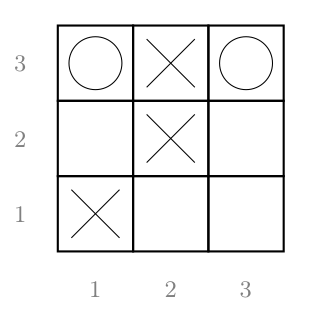
\includegraphics[width=8cm]{images/tikz1.png}  %%%%%%%%%%%%%%%%%%%%%%%%%%%
}{
\begin{tikzpicture}
[thick]
  \foreach \x in {1,2,3}
    \foreach \y in {1,2,3}
    {
      \draw (\x,\y) +(-.5,-.5) rectangle ++(.5,.5);
    }

  %\draw (1,3) node{\begin{footnotesize}\textcolor{black!50}{1,3}\end{footnotesize}};
  %\draw (3,1) node{\begin{footnotesize}\textcolor{black!50}{3,1}\end{footnotesize}};
  \draw (0,3) node{\begin{footnotesize}\textcolor{black!50}{3}\end{footnotesize}};
  \draw (0,2) node{\begin{footnotesize}\textcolor{black!50}{2}\end{footnotesize}};
  \draw (0,1) node{\begin{footnotesize}\textcolor{black!50}{1}\end{footnotesize}};
  \draw (3,0) node{\begin{footnotesize}\textcolor{black!50}{3}\end{footnotesize}};
  \draw (2,0) node{\begin{footnotesize}\textcolor{black!50}{2}\end{footnotesize}};
  \draw (1,0) node{\begin{footnotesize}\textcolor{black!50}{1}\end{footnotesize}};

  \draw (2,3) node{\tikz \draw (-.32,-.32) -- (.32,.32);};
  \draw (2,3) node{\tikz \draw (-.32,.32) -- (.32,-.32);};

  \draw (2,2) node{\tikz \draw (-.32,-.32) -- (.32,.32);};
  \draw (2,2) node{\tikz \draw (-.32,.32) -- (.32,-.32);};

  \draw (1,1) node{\tikz \draw (-.32,-.32) -- (.32,.32);};
  \draw (1,1) node{\tikz \draw (-.32,.32) -- (.32,-.32);};

  \draw (1,3) node{\tikz \draw (0,0) circle (10pt);};

  \draw (3,3) node{\tikz \draw (0,0) circle (10pt);};
\end{tikzpicture}
}
\caption{A Tic-tac-toe board position, in which it is the ``circles'' player's turn to play. The labeling explains the indexing (left to right, bottom to top, starting at 1) of the grid.}
\label{fig:TTT}
\end{center}
\end{figure}

\begin{figure}
%%%\hspace{-0.8cm}
\begin{center}
\ifthenelse{\equal{\myebookformat}{true}}{                   %%%%%%%%%%%%%%%%%%%%%%%%%%%
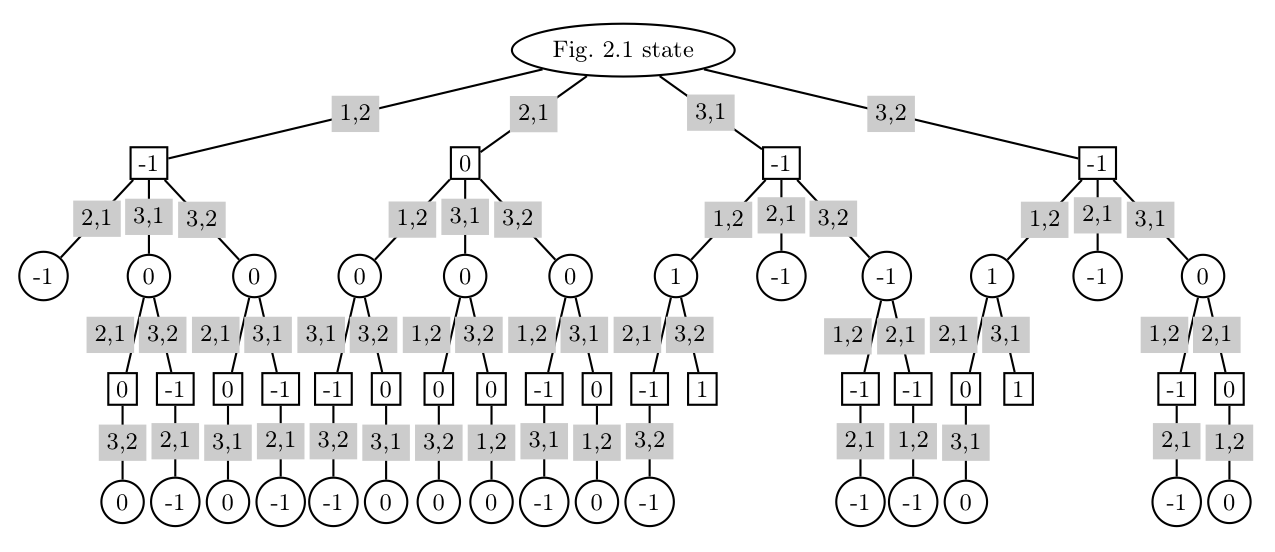
\includegraphics[width=8cm]{images/tikz2.png}  %%%%%%%%%%%%%%%%%%%%%%%%%%%
}{
\begin{tikzpicture}
    [thick,
level 1/.style={sibling distance=42mm},
level 2/.style={sibling distance=14mm},
level 3/.style={sibling distance=7mm}
]
\begin{footnotesize}
  \node[ellipse,draw] {Fig.~\ref{fig:TTT} state}
    child {node[rectangle,draw] {-1}
      child {node[circle,draw] {-1}
          edge from parent node[pos=0.5,fill=black!20] {2,1}
        }
      child {node[circle,draw] {0}
          child {node[rectangle,draw] {0}
              child {node[circle,draw] {0}
                edge from parent node[pos=0.5,fill=black!20] {3,2}}
              edge from parent node[pos=0.5,left,fill=black!20] {2,1}
            }
          child {node[rectangle,draw] {-1}
              child {node[circle,draw] {-1}
                edge from parent node[pos=0.5,fill=black!20] {2,1}}
              edge from parent node[pos=0.5,fill=black!20] {3,2}
            }
          edge from parent node[pos=0.5,fill=black!20] {3,1}
        }
      child {node[circle,draw] {0}
          child {node[rectangle,draw] {0}
              child {node[circle,draw] {0}
                edge from parent node[pos=0.5,fill=black!20] {3,1}}
              edge from parent node[pos=0.5,left,fill=black!20] {2,1}
            }
          child {node[rectangle,draw] {-1}
              child {node[circle,draw] {-1}
                edge from parent node[pos=0.5,fill=black!20] {2,1}}
              edge from parent node[pos=0.5,fill=black!20] {3,1}
            }
          edge from parent node[pos=0.5,fill=black!20] {3,2}
        }
      edge from parent node[pos=0.5,fill=black!20] {1,2}
    }
    child {node[rectangle,draw] {0}
      child {node[circle,draw] {0}
          child {node[rectangle,draw] {-1}
              child {node[circle,draw] {-1}
                edge from parent node[pos=0.5,fill=black!20] {3,2}}
              edge from parent node[pos=0.5,left,fill=black!20] {3,1}
            }
          child {node[rectangle,draw] {0}
              child {node[circle,draw] {0}
                edge from parent node[pos=0.5,fill=black!20] {3,1}}
              edge from parent node[pos=0.5,fill=black!20] {3,2}
            }
          edge from parent node[pos=0.5,fill=black!20] {1,2}
        }
      child {node[circle,draw] {0}
          child {node[rectangle,draw] {0}
              child {node[circle,draw] {0}
                edge from parent node[pos=0.5,fill=black!20] {3,2}}
              edge from parent node[pos=0.5,left,fill=black!20] {1,2}
            }
          child {node[rectangle,draw] {0}
              child {node[circle,draw] {0}
                edge from parent node[pos=0.5,fill=black!20] {1,2}}
              edge from parent node[pos=0.5,fill=black!20] {3,2}
            }
          edge from parent node[pos=0.5,fill=black!20] {3,1}
        }
      child {node[circle,draw] {0}
          child {node[rectangle,draw] {-1}
              child {node[circle,draw] {-1}
                edge from parent node[pos=0.5,fill=black!20] {3,1}}
              edge from parent node[pos=0.5,left,fill=black!20] {1,2}
            }
          child {node[rectangle,draw] {0}
              child {node[circle,draw] {0}
                edge from parent node[pos=0.5,fill=black!20] {1,2}}
              edge from parent node[pos=0.5,fill=black!20] {3,1}
            }
          edge from parent node[pos=0.5,fill=black!20] {3,2}
        }
      edge from parent node[pos=0.5,fill=black!20] {2,1}
    }
    child {node[rectangle,draw] {-1}
      child {node[circle,draw] {1}
          child {node[rectangle,draw] {-1}
              child {node[circle,draw] {-1}
                edge from parent node[pos=0.5,fill=black!20] {3,2}}
              edge from parent node[pos=0.5,left,fill=black!20] {2,1}
            }
          child {node[rectangle,draw] {1}
              edge from parent node[pos=0.5,fill=black!20] {3,2}
            }
          edge from parent node[pos=0.5,fill=black!20] {1,2}
        }
      child {node[circle,draw] {-1}
          edge from parent node[pos=0.5,fill=black!20] {2,1}
        }
      child {node[circle,draw] {-1}
          child {node[rectangle,draw] {-1}
              child {node[circle,draw] {-1}
                edge from parent node[pos=0.5,fill=black!20] {2,1}}
              edge from parent node[pos=0.5,left,fill=black!20] {1,2}
            }
          child {node[rectangle,draw] {-1}
              child {node[circle,draw] {-1}
                edge from parent node[pos=0.5,fill=black!20] {1,2}}
              edge from parent node[pos=0.5,fill=black!20] {2,1}
            }
          edge from parent node[pos=0.5,fill=black!20] {3,2}
        }
      edge from parent node[pos=0.5,fill=black!20] {3,1}
    }
    child {node[rectangle,draw] {-1}
      child {node[circle,draw] {1}
          child {node[rectangle,draw] {0}
              child {node[circle,draw] {0}
                edge from parent node[pos=0.5,fill=black!20] {3,1}}
              edge from parent node[pos=0.5,left,fill=black!20] {2,1}
            }
          child {node[rectangle,draw] {1}
              edge from parent node[pos=0.5,fill=black!20] {3,1}
            }
          edge from parent node[pos=0.5,fill=black!20] {1,2}
        }
      child {node[circle,draw] {-1}
          edge from parent node[pos=0.5,fill=black!20] {2,1}
        }
      child {node[circle,draw] {0}
          child {node[rectangle,draw] {-1}
              child {node[circle,draw] {-1}
                edge from parent node[pos=0.5,fill=black!20] {2,1}}
              edge from parent node[pos=0.5,left,fill=black!20] {1,2}
            }
          child {node[rectangle,draw] {0}
              child {node[circle,draw] {0}
                edge from parent node[pos=0.5,fill=black!20] {1,2}}
              edge from parent node[pos=0.5,fill=black!20] {2,1}
            }
          edge from parent node[pos=0.5,fill=black!20] {3,1}
        }
      edge from parent node[pos=0.5,fill=black!20] {3,2}
    };
\end{footnotesize}
\end{tikzpicture}
}
\end{center}
\caption{Minimax tree with initial position at Fig.~\ref{fig:TTT} state, \textbf{nodes} are states and \textbf{edges} are transitions, labeled with the move. Leafs are end-game states: 1 point for the win and -1 for the loss. Player is ``circles'' and plays first (first edges are player's moves).}
\label{fig:minimaxTTT}
\end{figure}
\subsection{Checkers, Alpha-beta}
Checkers, Chess and Go are also zero sum, \newglossaryentry{perfectinformation}{name={perfect-information},description={(game) in which all the players have complete knowledge of the (board) state of the game}}\glos{perfectinformation}, \newglossaryentry{partisan}{name={partisan},description={(game) which is not impartial, in which a player can do actions another can not do (move a faction while the other player(s) cannot)}}\glos{partisan}, deterministic strategy game. Theoretically, they all can be solved by exhaustive Minimax. 
In practice though, it is often intractable: their bounded versions are at least in \textsc{pspace} and their unbounded versions are \textsc{exptime}-hard \citep{GPC}. We can see the complexity of Minimax as $O(b^d)$ with $b$ the average branching factor of the tree (to search) and $d$ the average length (depth) of the game. 
For Checkers $b \approx 8$, but taking pieces is mandatory, resulting in a mean adjusted branching factor of $\approx 4$, while the mean game length is 70 resulting in a game tree complexity of $\approx 10^{31}$ \citep{allis1994}. It is already too large to have been solved by Minimax alone (on current hardware). From 1989 to 2007, there were artificial intelligences competitions on Checkers, all using at least alpha-beta pruning: a technique to make efficient cuts in the Minimax search tree while not losing optimality. 
The state space complexity of Checkers is the smallest of the 3 above-mentioned games with $\approx 5.10^{20}$ legal possible positions (conformations of pieces which can happen in games). As a matter of fact, Checkers have been (weakly) solved, which means it was solved for perfect perfect play on both sides (and always ends in a draw) \citep{Schaeffer07}. Not all positions resulting from imperfect play have been analyzed. 

Alpha-beta pruning (see Algorithm~\ref{alg:alphabeta}) is a branch-and-bound algorithm which can reduce Minimax search down to a $O(b^{d/2})=O(\sqrt{b^d})$ complexity if the best nodes are searched first ($O(b^{3d/4})$ for a random ordering of nodes). $\alpha$ is the maximum score than we (the maximizing player) are assured to get given what we already evaluated, while $\beta$ is the minimum score than the minimizing player is assured to get. When evaluating more and more nodes, we can only get a better estimate and so $\alpha$ can only increase while $\beta$ can only decrease. %If we find a node for us with an expected value below $\alpha$, we do not have to consider its subtree because it's sub-optimal play. If we find an expected value above $\beta$, it's sub-optimal play for the opponent. 
\begin{algorithm}
\caption{Alpha-beta algorithm}
\label{alg:alphabeta}
\begin{algorithmic}
\Function{alphabeta}{node,depth,$\alpha$,$\beta$,player}
    \If{$depth \leq 0$}
        \State \Return $value(player)$
    \EndIf
    \If{$player == us$}
        \ForAll{possible moves}
            \State $\alpha \gets \max{(\alpha, alphabeta(child,depth-1,\alpha,\beta,opponent))}$
            \If{$\beta \leq \alpha$}
                \State \textbf{break}
            \EndIf
        \EndFor
        \State \Return $\alpha$
    \Else
        \ForAll{possible moves}
            \State $\beta \gets \min{(\beta, alphabeta(child,depth-1,\alpha,\beta,us))}$
            \If{$\beta \leq \alpha$}
                \State \textbf{break}
            \EndIf
        \EndFor
        \State \Return $\beta$
    \EndIf
\EndFunction
\end{algorithmic}
\end{algorithm}
If we find a node for which $\beta$ becomes less than $\alpha$, it means that this position results from sub-optimal play. When it is because of an update of $\beta$, the sub-optimal play is on the side of the maximizing player (his $\alpha$ is not high enough to be optimal and/or the minimizing player has a winning move faster in the current sub-tree) and this situation is called an $\alpha$ cut-off. On the contrary, when the cut results from an update of $\alpha$, it is called a $\beta$ cut-off and means that the minimizing player would have to play sub-optimally to get into this sub-tree. When Starting the game, $\alpha$ is initialized to $-\infty$ and $\beta$ to $+\infty$. A worked example is given on Figure~\ref{fig:alphabeta}.
\tikzset{
alphacut/.style={postaction={decorate},
        decoration={markings,mark=at position .50 with {\draw (0.05,-.28)--(0.05,.28);\draw (-.05,-.28)--(-.05,.28);\node[right]{$\ \ \alpha \ cut$};}}},
betacut/.style={postaction={decorate},
        decoration={markings,mark=at position .50 with {\draw (0.05,-.28)--(0.05,.28);\draw (-.05,-.28)--(-.05,.28);\node[right]{$\ \ \beta \ cut$};}}},
}
\begin{figure}
%%%\hspace{-0.8cm}
\begin{center}
\ifthenelse{\equal{\myebookformat}{true}}{                   %%%%%%%%%%%%%%%%%%%%%%%%%%%
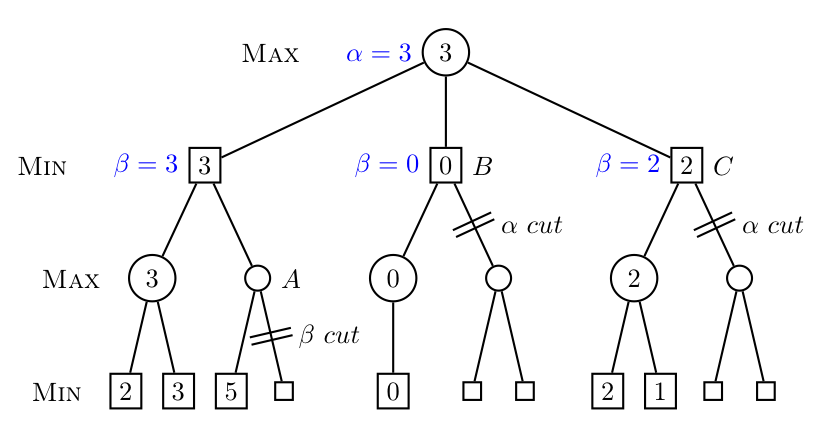
\includegraphics[width=8cm]{images/tikz3.png}  %%%%%%%%%%%%%%%%%%%%%%%%%%%
}{
\begin{tikzpicture}
    [thick,
level 1/.style={sibling distance=32mm},
level 2/.style={sibling distance=14mm},
level 3/.style={sibling distance=7mm}
]
\begin{small}
  \node[circle,draw] (top) {3}
    child {node[rectangle,draw] (a) {3}
        child {node[circle,draw] (d3) {3}
            child {node[rectangle,draw] (d4) {2}}
            child {node[rectangle,draw] {3}}
        }
        child {node[circle,draw] (A) {}
            child {node[rectangle,draw] {5}}
            child {node[rectangle,draw] {} edge from parent[betacut]}
        }
    }
    child {node[rectangle,draw] (b) {0}
        child {node[circle,draw] {0}
            child {node[rectangle,draw] {0}}
        }
        child {node[circle,draw] (B) {}
            child {node[rectangle,draw] {}}
            child {node[rectangle,draw] {}}
            edge from parent[alphacut]
        }
    }
    child {node[rectangle,draw] (c) {2}
        child {node[circle,draw] {2}
            child {node[rectangle,draw] {2}}
            child {node[rectangle,draw] {1}}
        }
        child {node[circle,draw] {}
            child {node[rectangle,draw] {}}
            child {node[rectangle,draw] {}}
            edge from parent[alphacut]
        }
    };
    \node [blue,left] at (top.west) (d1) {$\alpha = 3$};
    \node [blue,left] at (a.west) (d2) {$\beta = 3$};
    \node [blue,left] at (b.west) {$\beta = 0$};
    \node [blue,left] at (c.west) {$\beta = 2$};
    \node [right] at (A.east) {$A$};
    \node [right] at (b.east) {$B$};
    \node [right] at (c.east) {$C$};
    \node [left,align=flush left] at (d1.west) {\textsc{Max}\ \ \ };
    \node [left,align=flush left] at (d2.west) {\textsc{Min}\ \ \ };
    \node [left] at (d3.west) {\textsc{Max}\ \ \ };
    \node [left] at (d4.west) {\textsc{Min}\ \ \ };
\end{small}
\end{tikzpicture}
}
\end{center}
\caption{Alpha-beta cuts on a Minimax tree, \textbf{nodes} are states and \textbf{edges} are transitions, labeled with the values of positions at the bottom (max depth). Here is the trace of the algorithm: \textbf{1.} descend leftmost first and evaluated 2 and 3, \textbf{2.} percolate max(2,3) higher up to set $\beta = 3$, \textbf{3.} $\beta$-cut in $A$ because its value is at least 5 (which is superior to $\beta=3$), \textbf{4.} Update of $\alpha=3$ at the top node, \textbf{5.} $\alpha$-cut in $B$ because it is at most 0 (which is inferior to $\alpha=3$), \textbf{6.} $\alpha$-cut in $C$ because it is at most 2, \textbf{7.} conclude the best value for the top node is 3.}
\label{fig:alphabeta}
\end{figure}
%Prior to Checkers being solved (meaning that we have a database of which moves to play for all positions resulting from optimal play), or if playing against a sub-optimal opponent, 
Alpha-beta is going to be helpful to search much deeper than Minimax in the same allowed time. The best Checkers program (since the 90s), which is also the project which solved Checkers \citep{SchaefferBBKMLLS07}, Chinook, has openings and end-game (for lest than eight pieces of fewer) books, and for the mid-game (when there are more possible moves) relies on a deep search algorithm. So, appart for the beginning and the ending of the game, for which it plays by looking up a database, it used a search algorithm. As Minimax and Alpha-beta are depth first search heuristics, all programs which have to answer in a fixed limit of time use \textit{iterative deepening}, a technique which consists in fixing limited depth which will be considered maximal and evaluating this position. As it does not relies in winning moves at the bottom, because the search space is too big in $branching^{depth}$, we need moves evaluation heuristics. We then iterate on growing the maximal depth for which we consider moves, but we are at least sure to have a move to play in a short time (at least the greedy depth 1 found move).

\subsection{Chess, Heuristics}
With a branching factor of $\approx 35$ and an average game length of 80 moves \citep{Shannon_1950}, the average game-tree complexity of chess is $35^{80}\approx 3.10^{123}$. \citet{Shannon_1950} also estimated the number of possible (legal) positions to be of the order of $10^{43}$, which is called the Shannon number. Chess AI needed a little more than just Alpha-beta to win against top human players (not that Checkers could not benefit it), particularly on 1996 hardware (first win of a computer against a reigning world champion, Deep Blue vs. Garry Kasparov). Once an AI has openings and ending books (databases to look-up for classical moves), how can we search deeper during the game, or how can we evaluate better a situation? In iterative deepening Alpha-beta (or other search algorithms like Negascout \citep{reinfeld1983negascout} or MTD-f\citep{Plaat1996}), one needs to know the value of a move at the maximal depth. If it does not correspond to the end of the game, there is a need for a evaluation heuristic. Some may be straight forward, like the resulting value of an exchange in pieces points. But some strategies sacrifice a queen in favor of a more advantageous tactical position or a checkmate, so evaluation heuristics need to take tactical positions into account. In Deep Blue, the evaluation function had 8000 cases, with 4000 positions in the openings book, all learned from 700,000 grandmaster games \citep{DeepBlue}. Nowadays, Chess programs are better than deep blue and generally also search less positions. For instance, Pocket Fritz (HIARCS engine) beats current grandmasters \citep{PocketFritz,CopaMercosur} while evaluating 20,000 positions per second (740 MIPS on a smartphone) against Deep Blue's (11.38 GFlops) 200 millions per second.

\subsection{Go, Monte-Carlo Tree Search}
With an estimated number of legal 19x19 Go positions of $2.081681994 * 10^{170}$ \citep{tromp2006} (1.196\% of possible positions), and an average branching factor above Chess for \newglossaryentry{goban}{name=goban,description={board used for the game of Go},plural=gobans}\gloss{goban} from 9x9 and above, Go sets another limit for AI. For 19x19 gobans, the game tree complexity is up to $10^{360}$ \citep{allis1994}. The branching factor varies greatly, from $\approx 30$ to $300$ (361 cases at first), while the mean depth (number of plies in a game) is between 150 to 200. Approaches other than systematic exploration of the game tree are required. One of them is Monte Carlo Tree Search \newglossaryentry{MCTS}{name=MCTS,description={Monte-Carlo Tree Search}}(\glos{MCTS}). Its principle is to randomly sample which nodes to expand and which to exploit in the search tree, instead of systematically expanding the build tree as in Minimax. For a given $node$ in the search tree, we note $Q(node)$ the sum of the simulations rewards on all the runs through $node$, and $N(node)$ the visits count of $node$. Algorithm~\ref{alg:mcts} details the MCTS algorithm and Fig.~\ref{fig:MCTS} explains the principle.

\begin{algorithm}
\caption{Monte-Carlo Tree Search algorithm. 
\textsc{ExpandFrom}$(node)$ is the tree (growing) policy function on how to select where to search from situation $node$ (exploration or exploitation?) and how to expand the game tree (deep-first, breadth-first, heuristics?) in case of untried actions. \textsc{Evaluate}$(tree)$ may have 2 behaviors: \textbf{1.} if $tree$ is complete (terminal), it gives an evaluation according to games rules, \textbf{2.} if $tree$ is incomplete, it has to give an estimation, either through simulation (for instance play at random) or an heuristic. \textsc{BestChild} picks the action that leads to the better value/reward from $node$. \textsc{Merge}$(node, tree)$ changes the existing tree (with $node$) to take all the $Q(\nu) \forall \nu \in tree$ (new) values into account. If $tree$ contains new nodes (there were some exploration), they are added to $node$ at the right positions.}
\label{alg:mcts}
\begin{algorithmic}
\Function{MCTS}{$node$}
    \While{computational time left}
        \State $tree \gets$ \textsc{ExpandFrom}$(node)$
        \State $tree.values \gets$ \textsc{Evaluate}$(tree)$
        \State \textsc{Merge}$(node, tree)$
    \EndWhile
    \State \Return \textsc{BestChild}$(node)$
\EndFunction
\end{algorithmic}
\end{algorithm}


The MoGo team \citep{GellyUCT, Gelly2006} introduced Upper Confidence Bounds for Trees (\newglossaryentry{UCT}{name=UCT,description={Upper Confidence Bounds for Trees}}\glos{UCT}) for \glos{MCTS} in Go AI. MoGo became the best 9x9 and 13x13 Go program, and the first to win against a pro on 9x9. UCT specializes MCTS in that it specifies \textsc{ExpandFrom} (as in Algorithm.~\ref{alg:expandfrom}) tree policy with a specific exploration-exploitation trade-off. UCB1 \citep{BanditBased} views the tree policy as a multi-armed bandit problem and so \textsc{ExpandFrom}$(node)$ UCB1 chooses the arms with the best upper confidence bound: $$\argmax_{c \in node.children} \frac{Q(c)}{N(c)}+k\sqrt{\frac{\ln N(node)}{N(c)}}$$ in which $k$ fixes the exploration-exploitation trade-off: $\frac{Q(c)}{N(c)}$ is simply the average reward when going through $c$ so we have exploitation only for $k=0$ and exploration only for $k=\infty$.

\citet{BanditBased} showed that the probability of selecting sub-optimal actions converges to zero and so that UCT MCTS converges to the minimax tree and so is optimal. Empirically, they found several convergences rates of UCT to be in $O(b^{d/2})$, as fast as Alpha-beta tree search, and able to deal with larger problems (with some error). For a broader survey on MCTS methods, see \citep{MCTSsurvey}.

\begin{algorithm}
\caption{UCB1 \textsc{ExpandFrom}}
\label{alg:expandfrom}
\begin{algorithmic}
\Function{ExpandFrom}{$node$}
    \If{$node$ is terminal}
        \State \Return $node$ \ \ \ \ \texttt{// terminal}
    \EndIf
    \If{$\exists c \in node.children\ s.t.\ N(c)=0 $}
        \State \Return $c$ \ \ \ \ \texttt{// grow}
    \EndIf
    \State \Return \textsc{ExpandFrom}$(\argmax_{c \in node.children)} \frac{Q(c)}{N(c)}+k\sqrt{\frac{\ln N(node)}{N(c)}})$ \ \ \ \ \texttt{// select}
\EndFunction 
\end{algorithmic}
\end{algorithm}

\begin{figure}
\begin{center}
\tikzset{
%/.style={postaction={decorate},
%        decoration={markings,mark=at position .50 with {\draw (0.05,-.28)--(0.05,.28);\draw (-.05,-.28)--(-.05,.28);\node[right]{$\ \ \beta \ cut$};}}},
}
\ifthenelse{\equal{\myebookformat}{true}}{                   %%%%%%%%%%%%%%%%%%%%%%%%%%%
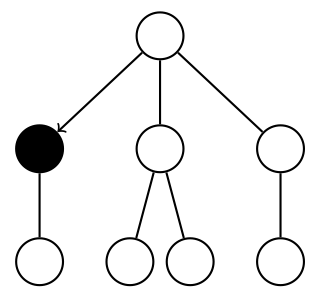
\includegraphics[width=5cm]{images/tikz4.png}  %%%%%%%%%%%%%%%%%%%%%%%%%%%
}{
\begin{tikzpicture}
[
thick,
level 1/.style={sibling distance=16mm},
level 2/.style={sibling distance=8mm}
]
\begin{footnotesize}
  \node[circle,draw,inner sep=2.2mm] {}
    child {node[circle,draw,inner sep=2.2mm,fill] {} edge from parent [->]
        child {node[circle,draw,inner sep=2.2mm] {} edge from parent [-]}
        %child {node[circle,draw] {}}
    }
    child {node[circle,draw,inner sep=2.2mm] {}
        child {node[circle,draw,inner sep=2.2mm] {}
        }
        child {node[circle,draw,inner sep=2.2mm] {}
        }
    }
    child {node[circle,draw,inner sep=2.2mm] {}
        child {node[circle,draw,inner sep=2.2mm] {}
        }
    };
\end{footnotesize}
\end{tikzpicture}
}
\hspace{1cm}
\ifthenelse{\equal{\myebookformat}{true}}{                   %%%%%%%%%%%%%%%%%%%%%%%%%%%
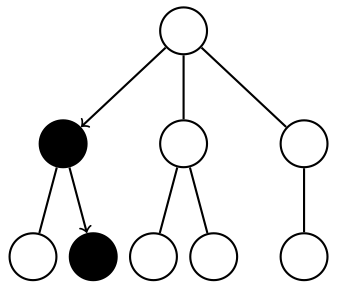
\includegraphics[width=5cm]{images/tikz5.png}  %%%%%%%%%%%%%%%%%%%%%%%%%%%
}{
\begin{tikzpicture}
[
thick,
level 1/.style={sibling distance=16mm},
level 2/.style={sibling distance=8mm}
]
\begin{footnotesize}
  \node[circle,draw,inner sep=2.2mm] {}
    child {node[circle,draw,inner sep=2.2mm,fill] {} edge from parent [->]
        child {node[circle,draw,inner sep=2.2mm] {} edge from parent [-]}
        child {node[circle,draw,inner sep=2.2mm,fill] {} edge from parent [->]}
        %child {node[circle,draw,inner sep=2.2mm] {}}
    }
    child {node[circle,draw,inner sep=2.2mm] {}
        child {node[circle,draw,inner sep=2.2mm] {}
        }
        child {node[circle,draw,inner sep=2.2mm] {}
        }
    }
    child {node[circle,draw,inner sep=2.2mm] {}
        child {node[circle,draw,inner sep=2.2mm] {}
        }
    };
\end{footnotesize}
\end{tikzpicture}
}
\hspace{1cm}

\ifthenelse{\equal{\myebookformat}{true}}{                   %%%%%%%%%%%%%%%%%%%%%%%%%%%
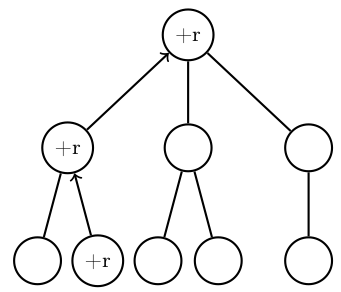
\includegraphics[width=5cm]{images/tikz6.png}  %%%%%%%%%%%%%%%%%%%%%%%%%%%
}{
\begin{tikzpicture}
[
thick,
level 1/.style={sibling distance=16mm},
level 2/.style={sibling distance=8mm}
]
\begin{scriptsize}
  \node[circle,draw] {+r}
    child {node[circle,draw] {+r} edge from parent [<-]
        child {node[circle,draw,inner sep=2.2mm] {} edge from parent [-]}
        child {node[circle,draw] {+r} edge from parent [<-]}
        %child {node[circle,draw] {}}
    }
    child {node[circle,draw,inner sep=2.2mm] {}
        child {node[circle,draw,inner sep=2.2mm] {}
        }
        child {node[circle,draw,inner sep=2.2mm] {}
        }
    }
    child {node[circle,draw,inner sep=2.2mm] {}
        child {node[circle,draw,inner sep=2.2mm] {}
        }
    };
\end{scriptsize}
\end{tikzpicture}
}
\caption{An iteration of the \textbf{while} loop in MCTS, from left to right:
\textsc{ExpandFrom} select, \textsc{ExpandFrom} grow, \textsc{Evaluate} \& \textsc{Merge}.}
\label{fig:MCTS}
\end{center}
\end{figure}

With Go, we see clearly that humans do not play abstract strategy games using the same approach. Top Go players can reason about their opponent's move, but they seem to be able to do it in a qualitative manner, at another scale. So, while tree search algorithms help a lot for tactical play in Go, particularly by integrating openings/ending knowledge, pattern macthing algorithms are not yet at the strategical level of human players. When a MCTS algorithm learns something, it stays at the level of possible actions (even considering \newglossaryentry{positionalhashing}{name={positional hashing},description={a method for determining similarities in (board) positions using hash functions}}\glos{positionalhashing}), while the human player seems to be able to generalize, and re-use heuristics learned at another level.

%%%%%%%%%%%%%%%%%%%%%%%%%%%%%%%%%%%%%%%%%%%%%%%%%%%%%%%%%%%%%%%%%% 

\section{Games with Uncertainty}
An exhaustive list of games or even of games genres is beyond the scope/range of this thesis. %On the other hand, we will explain games for which randomness or incomplete information plays a key role with not-so-basic examples. 
All uncertainty boils down to incompleteness of information, being it the physics of the dice being thrown or the inability to measure what is happening in the opponent's brain. However,  we will speak of 2 types (sources) of uncertainty: extensional uncertainty, which is due to incompleteness in direct, measurable information, and intentional uncertainty, which is related to randomness in the game or in (the opponent's) decisions. As extreme illustrations of this: an agent acting without sending is under full extensional uncertainty, while an agent whose acts are the results of a perfect random generator is under full intentional uncertainty. The uncertainty coming from the opponent's mind/cognition lies in between, depending on the simplicity to model the game as an optimization procedure. The harder the game is to model, the harder it is to model the trains of thoughts our opponents can follow.

\subsection{Monopoly}
In Monopoly, there is few hidden information (\textit{Chance} and \textit{Community Chest} cards only), but there is randomness in the throwing of dice\footnote{Note that the sum of two uniform distributions is not a uniform but a Irwin-Hall, $\forall n>1, \PP([\sum_{i=1}^n{(X_i\in U(0,1))}]=x) \propto \frac{1}{(n-1)!}\sum_{k=0}^n(-1)^k{n\choose k}\max{((x-k)^{n-1},0)}$, converging towards a Gaussian (central limit theorem).}, and a substantial influence of the player's knowledge of the game. A very basic playing strategy would be to just look at the ruturn on investment (ROI) with regard to prices, rents and frequencies, choosing only based on the money you have and the possible actions of buying or not. A less naive way to play should evaluate the questions of buying with regard to what we already own, what others own, our cash and advancement in the game. The complete state space is huge (places for each players $\times$ their money $\times$ their possessions), but according to \cite{MonopolyMarkov}, we can model the game for one player (as he has no influence on the dice rolls and decisions of others) as a Markov process on 120 ordered pairs: 40 board spaces $\times$ possible number of doubles rolled so far in this turn (0, 1, 2). With this model, it is possible to compute more than simple ROI and derive applicable and interesting strategies. So, even in monopoly, which is not lottery playing or simple dice throwing, a simple probabilistic modeling yields a robust strategy. Additionally, \cite{MonopolyFrayn05} used genetic algorithms to generate the most efficient strategies for portfolio management. %We observe that the main difficulty of Monopoly: randomness in a gameplay in which we have to make up a strategy, can be dealt with with probabilistic modeling. 

Monopoly is an example of a game in which we have complete direct information about the state of the game, intentional uncertainty due to the roll of the dice (randomness) can be dealt with thanks to probabilistic modeling (Markov processes here). The opponent's actions are relatively easy to model due to the fact that the goal is to maximize cash and that there are not many different efficient strategies (not many Nash equilibrium if it were a stricter game) to attain it. In general, the presence of chance does not invalidates previous (game theoretic / game trees) approaches but transforms exact computational techniques into stochastic ones: finite states machines become probabilistic Bayesian networks for instance.

%\subsection{Diplomacy}
%\subsection{Bridge}
\subsection{Battleship}
Battleship (also called ``naval combat'') is a guessing game generally played with two $10\times10$ grids for each players: one is the player's ships grid, and one is to remember/infer the opponent's ships positions. The goal is to guess where the enemy ships are and sink them by firing shots (torpedoes). There is \textbf{incompleteness} of information but no randomness. Incompleteness can be dealt with with probabilistic reasoning. The classic setup of the game consist in two ships of length 3 and one ship of each lengths of 2, 4 and 5; in this setup, there are 1,925,751,392 possible arrangements for the ships. The way to take advantage of all possible information is to update the probability that there is a ship for all the squares each time we have additional information. So for the $10\times10$ grid we have a $10\times10$ matrix $O_{1:10,1:10}$ with $O_{i,j} \in \{true,false\}$ being the $i$th row and $j$th column random variable of the case being occupied. With $ships$ being unsunk ships, we always have: $$\sum_{i,j}\PP(O_{i,j}=true) = \frac{\sum_{k\in ships}length(k)}{10 \times 10}$$ For instance for a ship of size 3 alone at the beginning we can have prior distributions on $O_{1:10,1:10}$ by looking at combinations of its placements (see Fig.~\ref{fig:battleship}). We can also have priors on where the opponent likes to place her ships. Then each round we will either hit or miss in $i,j$. When we hit, we know $\PP(O_{i,j}=true)=1.0$ and will have to revise the probabilities of surrounding areas, and everywhere if we learned the size of the ship, with possible placement of ships. If we did not sunk a ship, the probabilities of uncertain (not 0.0 or 1.0) positions around $i,j$ will be highered according to the sizes of remaining ships. If we miss, we know $\PP([O_{i,j}=false])=1.0$ and can also revise (lower) the surrounding probabilities, an example of that effect is shown in Fig.~\ref{fig:battleship}. 

Battleship is a game with few intensional uncertainty (no randomness), particularly because the goal quite strongly conditions the action (sink ships as fast as possible) but a large part of extensional uncertainty (incompleteness of direct information), which goes down rather quickly once we act, if we update a probabilistic model of the map/grid. If we compare Battleship to a variant in which we could see the adversary board, playing would be straightforward (just hit ships we know the position on the board), now in real Battleship we have to model our uncertainty due to the incompleteness of information, without even beginning to take into account the psychology of the opponent in placement as a prior. The cost of solving an imperfect information game increases greatly from its perfect information variant: it seems to be easier to model stochasticity (chance, a source of randomness) than to model a hidden (complex) system for which we only observe (indirect) effects.

\begin{figure}[h!]
\begin{center}
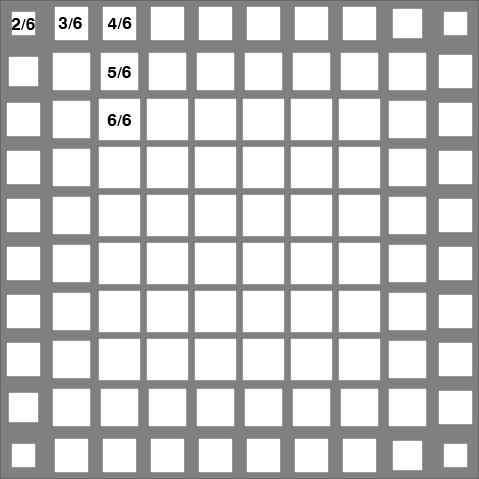
\includegraphics[width=7.8cm]{images/battleship_board_3_init_annotated.png} 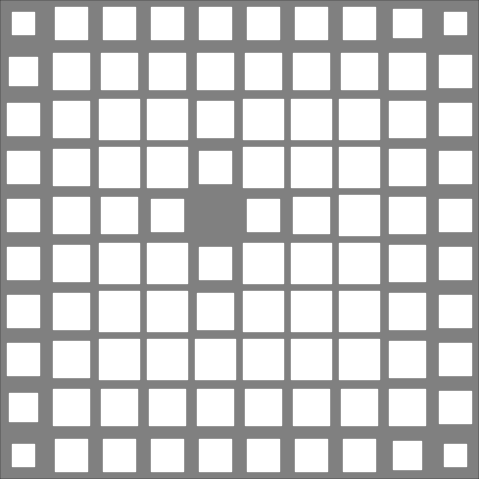
\includegraphics[width=7.8cm]{images/battleship_board_3_1miss.png}
\caption{Left: visualization of probabilities for squares to contain a ship of size 3 ($\PP(O_{i,j})=true$) initially, assuming uniform distribution of this type of ship. Annotations correspond to the \textit{number of combinations} (on six, the maximum number of conformations), Right: same probability after a miss in (5, 5). The larger the white area, the higher the probability.}
\label{fig:battleship}
\end{center}
\end{figure}


\subsection{Poker}
Poker\footnote{We deal mainly with the \textit{Limit Hold'em} variant of Poker.} is a zero-sum (without the house's cut), imperfect information and stochastic betting game. Poker ``AI'' is as old as game theory \citep{nash51a}, but the research effort for human-level Poker AI started in the end of the 90s. The interest for Poker AI is such that there are annual AAAI computer Poker competitions\footnote{\url{http://www.computerpokercompetition.org/}}. \citet{Billings98pokeras} defend Poker as an interesting game for decision-making research, %combining imperfect information with randomness. The
because the task of building a good/high level Poker AI (player) entails to take decisions with incomplete information about the state of the game, incomplete information about the opponents' intentions, and model their thoughts process to be able to bluff efficiently. A Bayesian network can combine these uncertainties and represent the player's hand, the opponents' hands and their playing behavior conditioned upon the hand, as in \citep{Korb99bayesianpoker}. A simple ``risk evaluating'' AI (folding and raising according to the outcomes of its hands) will not prevail against good human players. Bluffing, as described by \citet{VonNeumannMorgenstern1944} ``to create uncertainty in the opponent's mind'', is an element of Poker which needs its own modeling. \citet{Southey05bayesbluff} also give a Bayesian treatment to Poker, separating the uncertainty resulting from the game (draw of cards) and from the opponents' strategies, and focusing on bluff. From a game theoretic point of view, Poker is a \newglossaryentry{bayesiangame}{name={Bayesian game},description={a game in which information about knowledge about payoffs is incomplete}}\glos{bayesiangame}. In a Bayesian game, the normal form representation requires describing the strategy spaces, type spaces, payoff and belief functions for each player. It maps to all the possible game trees along with the agents' information state representing the probabilities of individual moves, called the extensive form. Both these forms scale very poorly (exponentially). \citet{Koller97representationsand} used the sequence form transformation, the set of realization weights of the sequences of moves\footnote{for a given player, a sequence is a path down the game tree isolating only moves under their control}, %of extensive form with informations sets,
to search over the space of randomized strategies for Bayesian games automatically. Unfortunately, strict game theoretic optimal strategies for full-scale Poker are still not tractable this way, two players Texas Hold'em having a state space $\approx O(10^{18})$. \citet{BillingsBDHSSS03} approximated the game-theoretic optimal strategies through abstraction and are able to beat strong human players (not world-class opponents).

Poker is a game with both extensional and intentional uncertainty, from the fact that the opponents' hands are hidden, the chance in the draw of the cards, the opponents' model about the game state and their model about our mental state(s) (leading our decision(s)). While the iterated reasoning (``if she does A, I can do B'') is (theoretically) finite in Chess due to perfect information, it is not the case in Poker (``I think she thinks I think...''). The combination of different sources of uncertainty (as in Poker) makes it complex to deal with it (somehow, the sources of uncertainty must be separated), and we will see that both these sources of uncertainties arise (at different levels) in video games.

%%%%%%%%%%%%%%%%%%%%%%%%%%%%%%%%%%%%%%%%%%%%%%%%%%%%%%%%%%%%%%%%%% 

\section{FPS}

\subsection{Gameplay and AI}
First person shooters \newglossaryentry{gameplay}{name=gameplay,description={describes the interactive aspects of game design, which constraints the players possible behaviors and the players' goals in a given game},plural=gameplays}\glos{gameplay} consist in controlling an agent in first person view, centered on the weapon, a gun for instance. The firsts FPS popular enough to bring the genre its name were Wolfeinstein 3D and Doom, by iD Software. Other classic FPS (series) include Duke Nukem 3D, Quake, Half-Life, Team Fortress, Counter-Strike, Unreal Tournament, Tribes, Halo, Medal of Honor, Call of Duty, Battlefield, etc. The distinction between ``fast FPS'' (e.g. Quake series, Unreal Tournament series) and others is made on the speed at which the player moves. In ``fast FPS'', the player is always jumping, running much faster and playing more in 3 dimensions than on discretely separate 2D ground planes. Game types include (but are not limited to):
\begin{itemize}
    \item single-player missions, depending of the game design.
    \item capture-the-flag (CTF), in which a player has to take the flag inside the enemy camp and bring it back in her own base.
    \item free-for-all (FFA), in which there are no alliances.
    \item team deathmatch (TD), in which two (or more) teams fight on score.
    \item various gather and escort (including hostage or payload modes), in which one team has to find and escort something/somebody to another location.
    \item duel/tournament/deathmatch, 1 vs 1 matches (mainly ``fast FPS'').
\end{itemize}
From these various game types, the player has to maximize its damage (or positive actions) output while staying alive. For that, she will navigate her avatar in an uncertain environment (partial information and other players intentions) and shoot (or not) at targets with specific weapons.

Some games allow for instant (or delayed, but asynchronous to other players) respawn (recreation/rebirth of a player), most likely in the ``fast FPS'' (Quake-like) games, while in others, the player has to wait for the end of the round to respawn. In some games, weapons, ammunitions, health, armor and items can be picked on the ground (mainly ``fast FPS''), in others, they are fixed at the start or can be bought in game (with points). The map design can make the gameplay vary a lot, between indoors, outdoors, arena-like or linear maps. According to maps and gameplay styles, combat may be well-prepared with ambushes, sniping, indirect (zone damages), or close proximity (even to fist weapons). Most often, there are strong tactical positions and effective ways to attack them. 

While ``skill'' (speed of the movements, accuracy of the shots) is easy to emulate for an AI, team-play is much harder for bots and it is always a key ability. Team-play is the combination of distributed evaluation of the situation, planning and distribution of specialized tasks. Very high skill also requires integrating over enemy's tactical plans and positions to be able to take indirect shots (grenades for instance) or better positioning (coming from their back), which is hard for AI too. An example of that is that very good human players consistently beat the best bots (nearing 100\% accuracy) in Quake III (which is an almost pure skill ``fast FPS''), because they take advantage of being seen just when their weapons reload or come from their back. Finally, bots which equal the humans by a higher accuracy are less fun to play with: it is a frustrating experience to be shot across the map, by a bot which was stuck in the door because it was pushed out of its trail.

\subsubsection{State of the art}

FPS AI consists in controlling an agent in a complex world: it can have to walk, run, crouch, jump, swim, interact with the environment and tools, and sometimes even fly. Additionally, it has to shoot at moving, coordinated and dangerous, targets. %The first solution, in Wolfeinstein 3D, was to have enemies just shoot or run towards the player. The game was basically a linear indoors two-dimensional (no jumps, no stairs, nor the possibility to shoot up or down) labyrinth. 
On a higher level, it may have to gather weapons, items or power-ups (health, armor, etc.), find interesting tactical locations, attack, chase, retreat...

The Quake III AI is a standard for Quake-like games \citep{waveren-02-artificial}. It consists in a layered architecture (hierarchical) FSM. At the sensory-motor level, it has an Area Awareness System (AAS) which detects collisions, accessibility and computes paths. The level above provides intelligence for chat, goals (locations to go to), goals and weapons selection through fuzzy logic. Higher up, there are the behavior FSM (``seek goals'', chase, retreat, fight, stand...) and production rules (if-then-else) for squad/team AI and orders. A team of bots always behaves following the orders of one of the bots. Bots have different natures and tempers, which can be accessed/felt by human players, specified by fuzzy relations on ``how much the bot wants to do, have, or use something''. A genetic algorithm was used to optimize the fuzzy logic parameters for specific purposes (like performance). This bot is fun to play against and is considered a success, however Quake-like games makes it easy to have high level bots because very good players have high accuracy (no fire spreading), so they do not feel cheated if bots have a high accuracy too. Also, the game is mainly indoors, which facilitates tactics and terrain reasoning. Finally, cooperative behaviors are not very evolved and consist in acting together towards a goal, not with specialized behaviors for each agent.

The more recent FPS games have dealt with these limitations by using combinations of STRIPS planning (F.E.A.R. \citep{orkinGDC_FEAR}), hierarchical task networks (HTN) (Killzone 2 \citep{Killzone2_HTN} and ArmA \citep{ArmA1_HTN}), Behavior trees (Halo 2 \citep{Isla}). Left4Dead (a cooperative PvE FPS) uses a global supervisor of the AI to set the pace of the threat to be the most enjoyable for the player \citep{left4dead2009}.% (Crysis2 BF3)
%\begin{color}{red}explain Behavior trees? \\
%\url{http://files.aigamedev.com/insiders/BehaviorTrees_Slides.pdf}\\ 
%\url{http://altdevblogaday.com/2011/02/24/introduction-to-behavior-trees/}\\
%\url{http://aigamedev.com/open/article/anatomy-ai-architecture/}\\
%\url{http://www.cgf-ai.com/docs/straatman_remco_killzone_ai.pdf} \end{color}

In research, \citet{Laird01} focused on learning rules for opponent modeling, planning and reactive planning (on Quake), so that the robot builds plan by anticipating the opponent's actions. \citet{LeHy04,theseRonan} used robotics inspired Bayesian models to quickly learn the parameters from human players (on Unreal Tournament). \citet{Zanetti2004} and \citet{westraQ3} applied evolutionary neural networks to optimize Quake III bots. Predicting opponents positions is a central task to believability and has been solved successfully using particle filters \citep{particlefiltergameAI} and other models (like Hidden Semi-Markov Models) \citep{Hladky_anevaluation}. Multi-objective neuro-evolution \citep{Zanetti2004,schrum_cig11competition} combines learning from human traces with evolutionary learning for the structure of the artificial neural network, and leads to realistic (human-like) behaviors, in the context of the BotPrize challenge (judged by humans) \citep{Hingston_2009}.

\subsubsection{Challenges}

Single-player FPS campaigns immersion could benefit from more realistic bots and clever squad tactics. Multi-player FPS are competitive games, and a better game AI should focus on:
\begin{itemize}
    \item \textbf{believability} requires the AI to take decisions with the same informations than the human player (fairness) and to be able to deal with unknown situation.
    \item \textbf{surprise} and {unpredictability} is key for both performance and the long-term interest in the human player in the AI.
    \item \textbf{performance}, to give a challenge to human players, can be achieved through cooperative, planned and specialized behaviors.
\end{itemize}

%%%%%%%%%%%%%%%%%%%%%%%%%%%%%%%%%%%%%%%%%%%%%%%%%%%%%%%%%%%%%%%%%% 

\section{(MMO)RPG}

\subsection{Gameplay and AI}
Inspired directly by tabletop and live action role-playing games (Dungeon \& Dragons) as new tools for the game masters, it is quite natural for the RPG to have ended up on computers. The firsts digital RPG were text (Wumpus) or ASCII-art (Rogue, NetHack) based. The gameplay evolved considerably with the technique. Nowadays, what we will call a role playing game (RPG) consist in the incarnation by the human player of an avatar (or a team of avatars) with a class: warrior, wizard, rogue, priest, etc., having different skills, spells, items, health points, stamina/energy/mana (magic energy) points. Generally, the story brings the player to solve puzzles and fight. In a fight, the player has to take decisions about what to do but plays a lesser role in performing the action than in a FPS game. In a FPS, she has to move the character (egocentrically) and aim to shoot; in a RPG, she has to position itself (often way less precisely and continually) and just decide which ability to use on which target (or a little more for ``action RPG''). Classic RPG include: Fallout, The Elders Scrolls (from Arena to Skyrim), Secret of Mana, Zelda, Final Fantasy, Diablo, Baldur's Gate. A MMORPG (e.g. World of Warcraft, AION or EVE Online) consist in a role-playing game in a persistent, multi-player world. There usually are players-run factions fighting each others’ (PvP) and players versus environment (PvE) situations. \\glos{PvE} may be a cooperative task in which human players fight together against different NPC, and in which the cooperation is at the center of the gameplay. PvP is also a cooperative task, but more policy and reactions-based than a trained and learned choregraphy as for PvE. We can distinguish three types (or modality) of NPC which have different game AI needs:
\begin{itemize}
    \item world/neutral/civilian NPC: gives quests, takes part in the world's or game's story, talks,
    \item ``mob''/hostile NPC that the player will fight, 
    \item ``pets''/allied NPC: acts by the players' sides.
    \item persistent character AI could maintain the players' avatars in the world when they are disconnected.
\end{itemize}
NPC acting strangely are sometimes worse for the player's immersion than immobile and dull ones. However, it is more fun for the player to battle with hostile NPC which are not too dumb or predictable. Players really expect allied NPC to at least not hinder them, and it is even better when they adapt to what the player is doing. %Finally, for MMORPG, persistent character AI could maintain the player's avatar in the world when she is enjoying real-life.

\subsubsection{State of the art}

Methods used in \glos{FPS} are also used in \glos{RPG}. The needs are sometimes a little different for RPG games, for instance RPG need interruptible behaviors, behaviors that can be stopped and resumed (dialogs, quests, fights...) that is. RPG also require stronger story-telling capabilities than other gameplay genres, for which they use (logical) story representations (ontologies) \citep{kline2009,riedl11}. Behavior multi-queues \citep{Cutumisu09} resolve the problems of having resumable, collaborative, real-time and parallel behavior, and tested their approach on Neverwinter Nights. Basically they use prioritized behavior queues which can be inserted (for interruption and resumption) in each others. AI directors are control programs tuning the difficulty and pace of the game session in real-time from player's metrics. \citet{kline2011} used an AI director to adapt the difficulty of Dark Spore to the performance (interactions and score) of the player in real-time.

\subsubsection{Challenges}

There are mainly two axes for RPG games to bring more fun: interest in the game play(s), and immersion. For both these topics, we think game AI can bring a lot:
\begin{itemize}
    \item \textbf{believability} of the agents will come from AI approaches than can deal with new situations, being it because they were not dealt with during game development (because the ``possible situations'' space is too big) or because they were brought by the players' unforeseeable actions. Scripts and strict policies approaches will be in difficulty here. %, and we will assist to other Skyrim's NPC blunders.
    \item \textbf{interest} (as opposed to boredom) for the human players in the game style of the AI will come from approaches which can generate different behaviors in a given situation. Expectable AI particularly affects replayability negatively.
    \item \textbf{performance} relative to the gameplay will come from AI approaches than can fully deal with cooperative behavior. One solution is to design mobs to be orders of magnitude stronger (in term of hit points and damages) than players characters, or more numerous. Another, arguably more entertaining, solution is to bring the mobs behavior to a point where they are a challenge for the team of human players.
\end{itemize}
Both believability and performance require to deal with uncertainty of the game environment. RPG AI problem spaces are not tractable for a frontal (low-level) search approach nor are there few enough situations to consider to just write a bunch of script and puppeteer artificial agents at any time.

%%%%%%%%%%%%%%%%%%%%%%%%%%%%%%%%%%%%%%%%%%%%%%%%%%%%%%%%%%%%%%%%%% 

\section{RTS}
As RTS are the central focus on this thesis, we will discuss specific problems and solution more in depth in their dedicated chapters, simply brushing here the underlying major research problems. Major RTS include the Command\&Conquer, Warcraft, StarCraft, Age of Empires and Total Annihilation series.

\subsection{Gameplay and AI}
RTS gameplay consist in gathering resources, building up an economic and military power through growth and technology, to defeat your opponent by destroying his base, army and economy. It requires dealing with strategy, tactics, and units management (often called micro-management) in real-time. Strategy consist in what will be done in the long term as well as predicting what the enemy is doing. It particularly deals with the economy/army trade-off estimation, army composition, long-term planning. The three aggregate indicators for strategy are aggression, production, and technology. The tactical aspect of the gameplay is dominated by military moves: when, where (with regard to topography and weak points), how to attack or defend. This implies dealing with \textit{extensional} (what the invisible units under ``\glos{fogofwar}'' are doing) and \textit{intentional} (what will the visible enemy units do) uncertainty. Finally, at the actions/motor level, micro-management is the art of maximizing the effectiveness of the units \textit{i.e.} the damages given/damages received ratio. For instance: retreat and save a wounded unit so that the enemy units would have to chase it either boosts your firepower or weakens the opponent's. Both \citep{Human-LevelAIKillerApplication} and \cite{gunn} propose that RTS AI is one of the most challenging genres, because all levels in the hierarchy of decisions are of importance.
%%% incompleteness of information yielding uncertainty

More will be said about RTS in the dedicated chapter~\ref{chapter:rtsai}.

\subsubsection{State of the art \& Challenges}
\citet{Buro04callfor} called for AI research in RTS games and identified the technical challenges as:% adversarial planning under uncertainty, learning and opponent modeling, and spatial and temporal reasoning.  

%On planning under uncertainty, \citet{LTW} used \newacronym{cbr}{CBR}{case-based reasoning}\glos{cbr} to perform dynamic plan retrieval extracted from domain knowledge in Wargus (Warcraft II clone). \citet{Ontanon2007} based their real-time case-based planning (CBP) system on a plan dependency graph which is learned from human demonstration in Wargus. In \citep{Mishra2008,Ontanon2010,metalevelbehavioradaptrts}, they used a knowledge-based approach to perform situation assessment to use the right plan, and revise it (integrating learning, planning, and problem solving in CBR), performing runtime adaptation by monitoring its performance. \citet{Trusty2011} used a genetic-algorithm inspired method to mix and optimize existing expert plan, also in Wargus. \citet{Chung05} adapted Monte-Carlo tree search to planning in RTS games and applied it to a capture-the-flag mod of Open RTS. \citet{UCT} applied UCT (MCTS algorithm) to tactical assault planning in Wargus. Reactive planning and goal-driven autonomy (that is, find the more relevant goal to follow in unknown situations) are studied in \citep{Weber2010cr,WeberCIG10}. \citet{Churchill2011} used abstractions and heuristics to produce a real-time build-order planner. %\citet{CadenaG11} used fuzzy CBR for strategic and tactical planning.
%\citep{Weber2010qf}

%On learning and opponent modeling, \citet{schadd2007opponent} used hierarchical classifiers to learn the opponent's behavior in Spring (an open source clone of Total Annihilation). \citet{HsiehS08} learned players' strategy models with CBR by mining replays of StarCraft. \citet{weberStrat} applied data-mining to StarCraft replays to learn to predict strategies. \citet{HagelbackCIG10} performed a study on what are the human like characteristics of play in RTS games. \citet{Kim2010} clusterized build-orders to learn them from replays. \citet{Kabanza2010} studied strategic and tactic plan and intent recognition by probabilistic weighting of plans from a plan library, on StarCraft. In \citep{SYNNAEVE:OpeningPred}, we clusterized replays to annotate them with openings (strategies) and then learned the parameters of a predictive Bayesian model for strategies from StarCraft replays. In \citep{SYNNAEVE:StratPred}, we also learned parameters of a strategy prediction Bayesian model from StarCraft replays but in an unsupervised fashion (predicting build/tech trees). \citet{HMMstrat_RTS_AIIDE11} also had an unsupervised learning approach by fitting HMM to players build actions (from StarCraft replays) and clustering the most probable HMM transitions to be subsets of strategies.

%On spatial and temporal reasoning, \citet{Forbus2002} presented tactical qualitative description of terrain for wargames through geometric and pathfinding analysis. \citet{Perkins2010} automatically extracted choke points and regions of StarCraft maps from a pruned Voronoi diagram. \citet{Southey2007} infered ``complex agent motions from partial information'' using hidden semi-markov models including A* as a motion model. \citet{ButlerCIG10} applied forward and inverse models simulation to the prediction of units movements from partial observations onto a RTS. \citet{weber2011aiide} implemented a simpler particle filter for state estimation in StarCraft. \citet{SORTS} used a cognitive approach mimicking human attention for tactics and units control. \citet{Miles2007} and \citet{SmithCIG10} co-evolved influence map trees for spatial (tactical) reasoning in RTS games. \citet{IntelligentMoving} combined flocking \citep{Reynolds1987} with influence maps, while \citet{teamCompositionRTS} enhanced it, supporting team composition and maneuvering by learning a self-organizing map. \citet{Hagelback2009} presented a multi-agent potential field based bot and we presented a similar unifying Bayesian model for micro-management \citep{SYNNAEVE:Micro} in which units are attracted or repulsed by different real or virtual units or goals.
% \citet{NovaBot2011}

%\subsubsection{Challenges}

%In \citep{Buro04callfor}, the challenges of RTS AI are:
\begin{itemize}
    \item \textbf{adversarial planning under uncertainty}, and for that abstractions have to be found both allowing to deal with partial observations and to plan in real-time.
    \item \textbf{learning and opponent modeling}: adaptivity plays a key role in the strength of human players.
    \item \textbf{spatial and temporal reasoning}: tactics using the terrain features and good timings are essential for higher level play.
\end{itemize}
To these challenges, we would like to add the difficulty of inter-connecting all special cases resolutions of these problems: both for the collaborative (economical and logistical) management of the resources, and for the sharing of uncertainty quantization in the decision-making processes. Collaborative management of the resources require arbitrage between sub-models on resources repartition. By sharing information (and its uncertainty) between sub-models, decisions can be made that account better for the whole knowledge of the AI system. This will be extended further in the next chapters as RTS are the main focus of this thesis.

%%%%%%%%%%%%%%%%%%%%%%%%%%%%%%%%%%%%%%%%%%%%%%%%%%%%%%%%%%%%%%%%%% 

\section{Games Characteristics}
All the types of video games that we saw before require to deal with imperfect information and sometimes with randomness, while elaborating a strategy (possibly from underlying policies). From a game theoretic point of view, these video games are close to what is called a \glos{bayesiangame} \citep{osborne-rubinstein}. %%% Their formal description is:
%%% \begin{itemize}
%%% \item $N$, a finite set of players,
%%% \item $\Omega$, a finite set of states,
%%% \end{itemize}
%%% $$\forall \mathrm{player}\ i \in N$$
%%% \begin{itemize}
%%% \item $A_i$, a set of actions,
%%% \item $T_i$, a set of signals that can be observed by $i$,
%%% \item $p_i$, a probability measure on $\Omega$ (prior belief of $i$),
%%% \item $\succ_i$, a preference relation on the set of probability measures over $A\times \Omega$ with $A = \times_{j \in N}A_j$.
%%% \end{itemize}
However, solving Bayesian games is non-trivial, there are no generic and efficient approaches, and so it has not been done formally for card games with more than a few cards. \citet{BillingsBDHSSS03} approximated a game theoretic solution for Poker through abstraction heuristics, it leads to believe than game theory can be applied at the higher (strategic) abstracted levels of video games.

We do not pretend to do a complete taxonomy of video games and AI (e.g. \citep{gunn}), but we wish to provide all the major informations to differentiate game genres (gameplays). To grasp the challenges they pose, we will provide abstract measures of complexity.

\subsection{Combinatory}
``How does the state of possible actions grow?'' To measure this, we used a measure from perfect information zero-sum games (as Checkers, Chess and Go): the branching factor $b$ and the depth $d$ of a typical game. The complexity of a game (for taking a decision) is proportional to $b^d$. The average branching factor for a board game is easy to compute: it is the average number of possible moves for a given player. For Poker, we set $b=3$ for \textit{fold, check} and \textit{raise}. $d$ should then be defined over some time, the average number of events (decisions) per hour in Poker is between $20$ to $240$. For video-games, we defined $b$ to be the average number of possible moves at each decision, so for ``continuous'' or ``real-time'' games it is some kind of function of the useful discretization of the virtual world at hand. $d$ has to be defined as a frequency at which a player (artificial or not) has to take decisions to be competitive in the game, so we will give it in $d/time\_unit$. For instance, for a car (plane) racing game, $b \approx 50-500$ because $b$ is a combination of throttle ($\ddot{x}$) and direction ($\theta$) sampled values that are relevant for the game world, with $d/min$ at least $60$: a player needs to correct her trajectory \textit{at least} once a second. In RTS games, $b \approx 200$ is a lower bound (in StarCraft we may have between $50$ to $400$ units to control), and very good amateurs and professional players perform more than $300$ actions per minute.

The sheer size of $b$ and $d$ in video games make it seem intractable, but humans are able to play, and to play well. To explain this phenomenon, we introduce ``vertical'' and ``horizontal'' continuities in decision making. Fig.~\ref{fig:abstractdecisionhierarchy} shows how one can view the decision-making process in a video game: at different time scales, the player has to choose between strategies to follow, that can be realized with the help of different tactics. Finally, at the action/output/motor level, these tactics have to be implemented one way or another. So, matching Fig.~\ref{fig:abstractdecisionhierarchy}, we could design a Bayesian model:
\begin{itemize}
\item $S^{t,t-1} \in {Attack,Defend,Collect,Hide}$, the strategy variable
\item $T^{t,t-1} \in {Front,Back,Hit-and-run,Infiltrate}$, the tactics variable
%\item $S^{t,t-1} \in {Attack,Defend,Seach,Hide}$, the strategy variable
%\item $T^{t,t-1} \in {Front,Back,Prepare,Rush}$, the tactics variable
\item $A^{t,t-1} \in {low\_level\_actions}$, the actions variable
\item $O_{1:n}^{t} \in \{observations\}$, the set of observations variables
\end{itemize}
%\begin{eqnarray*}
$$\PP(S^{t,t-1},T^{t,t-1},A^{t,t-1},O_{1:n}^t) = \PP(S^{t-1}).\PP(T^{t-1}).\PP(A^{t-1})$$
$$.\PP(O_{1:n}^t).\PP(S^t|S^{t-1},O_{1:n}^t).\PP(T^t|S^t,T^{t-1},O_{1:n}^t).\PP(A^t|T^t,A^{t-1},O_{1:n}^t)$$
\begin{itemize}
    \item $\PP(S^t|S^{t-1},O_{1:n}^t)$ should be read as ``the probability distribution on the strategies at time $t$ is determined/influenced by the strategy at time $t-1$ and the observations at time $t$''.
    \item $\PP(T^t|S^t,T^{t-1},O_{1:n}^t)$ should be read as ``the probability distribution on the tactics at time $t$ is determined by the strategy at time $t$, tactics at time $t-1$ and the observations at time $t$''.
    \item $\PP(A^t|T^t,A^{t-1},O_{1:n}^t)$ should be read as ``the probability distribution on the actions at time $t$ is determined by tactics at time $t$, the actions at time $t-1$ and the observations at time $t$''.
\end{itemize}
%\end{eqnarray*}

\begin{figure}
%%%\hspace{-0.8cm}
\begin{center}
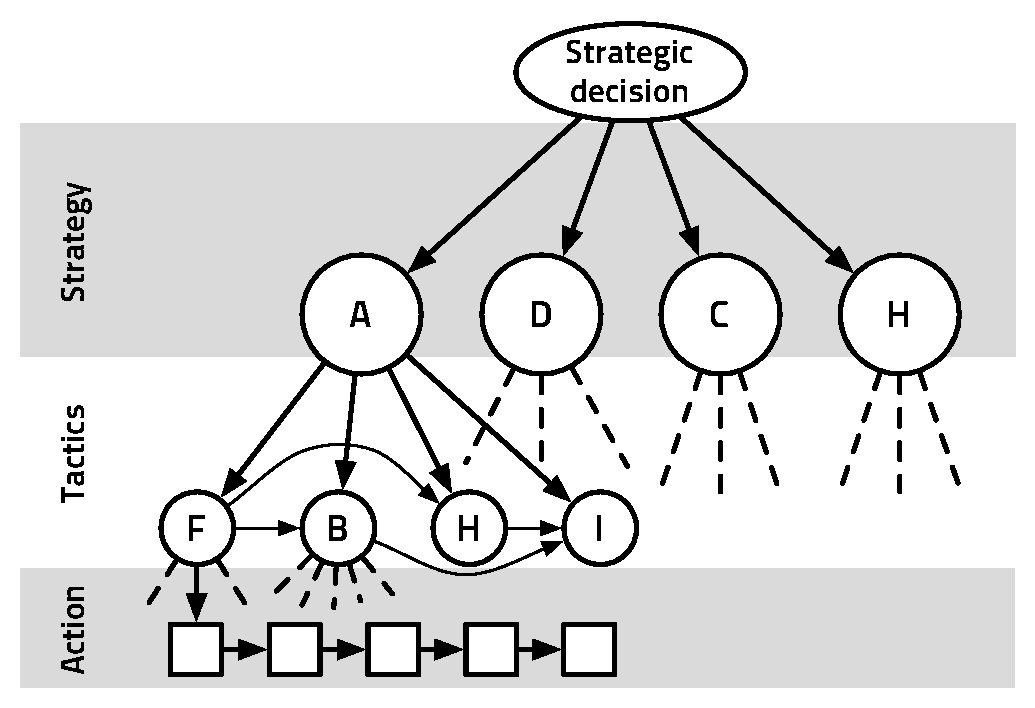
\includegraphics[width=10cm]{images/basic_abstract_decision_hierarchy3.pdf}
\end{center}
\caption{Abstract decision hierarchy in a video game. It is segmented in abstraction levels: at the strategical level, a decision is taken in $Attack$, $Defend$, $Collect$ and $Hide$; at the tactical level, it is decided between $Front$, $Back$, $Hit-and-run$, $Infiltrate$; and at the actions level between the player's possible interactions with the world.}
\label{fig:abstractdecisionhierarchy}
\end{figure}

\subsubsection{Vertical continuity}
In the decision-making process, vertical continuity describes when taking a higher-level decision implies a strong conditioning on lower-levels decisions. As seen on Figure~\ref{fig:verticalcont}: higher level abstractions have a strong conditioning on lower levels. For instance, and in non-probabilistic terms, if the choice of a strategy $s$ (in the domain of $S$) entails a strong reduction in the size of the domain of $T$, we consider that there is a vertical continuity between $S$ and $T$. There is vertical continuity between $S$ and $T$ if $\forall s \in \{S\}, \{\PP(T^t|[S^t=s], T^{t-1}, O_{1:n}^t) > \epsilon\}$ is sparse in $\{\PP(T^t|T^{t-1}, O_{1:n}^t) > \epsilon\}$. There can be local vertical continuity, for which the previous statement holds only for one (or a few) $s \in \{S\}$, which are harder to exploit. Recognizing vertical continuity allows us to explore the state space efficiently, filtering out absurd considerations with regard to the higher decision level(s).

\begin{figure}
%%%\hspace{-0.8cm}
\begin{center}
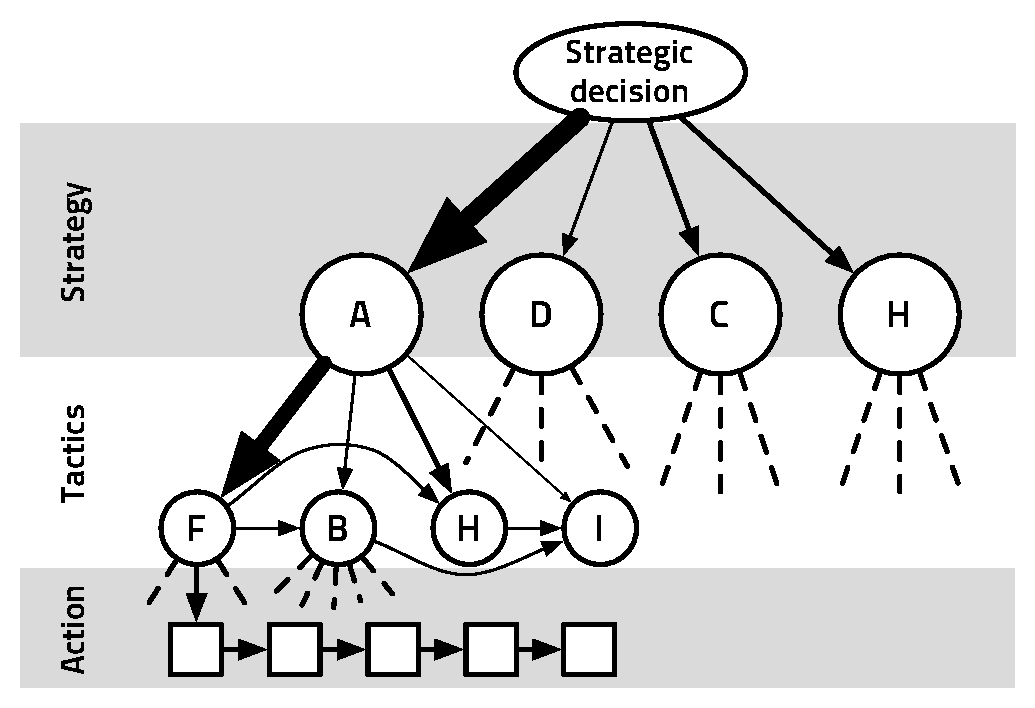
\includegraphics[width=10cm]{images/vertical_cont_abstract_decision_hierarchy3.pdf}
\end{center}
\caption{Vertical continuity in decision-making in a video game. There is a high vertical continuity between strategy and tactics as $\PP([T^t=Front]|[S^t=Attack], T^{t-1}, O_{1:n}^t)$ is much higher than other values for $\PP(T^t|S^t,T^{t-1},O_{1:n}^t)$. The thicker the arrow, the higher the transition probability.}
\label{fig:verticalcont}
\end{figure}

Examples? To edit, to choose with Pierre, ideas (+ point out example ``filtering out''):\\
navigation: S=always go north, T -> limited\\
whatever 2 player game: S=imitate, T -> limited\\
RTS: S=short term win by all-in, T -> limited\\
simpler examples?


\subsubsection{Horizontal continuity}
Horizontal continuity also helps out cutting the search in the state space to only relevant states. At a given abstraction level, it describes when taking a decision implies a strong conditioning on the next time-step decision (for this given level). As seen on Figure~\ref{fig:horizontalcont}: previous decisions on a given level have a strong conditioning on the next ones. For instance, and in non-probabilistic terms, if the choice of a tactic $t$ (in the domain of $T^t$) entails a strong reduction in the size of the domain of $T^{t+1}$, we consider that $T$ has horizontal continuity. There is horizontal continuity between $T^{t-1}$ and $T^t$ if $\forall t \in \{T\}, \{\PP(T^t|S^t,[T^{t-1}=t],O_{1:n}^t) > \epsilon\}$ is sparse in $\{\PP(T^t|S^t,O_{1:n}^t) > \epsilon\}$. There can be local horizontal continuity, for which the previous state holds only for one (or a few) $t \in \{T\}$. Recognizing horizontal continuity boils down to recognizing sequences of (frequent) actions from decisions/actions dynamics and use that to reduce the search space of subsequent decisions. Of course, at a sufficiently small time-step, most continuous games have high horizontal continuity: the size of the time-step is strongly related to the design of the abstraction levels for vertical continuity.

\begin{figure}
%%%\hspace{-0.8cm}
\begin{center}
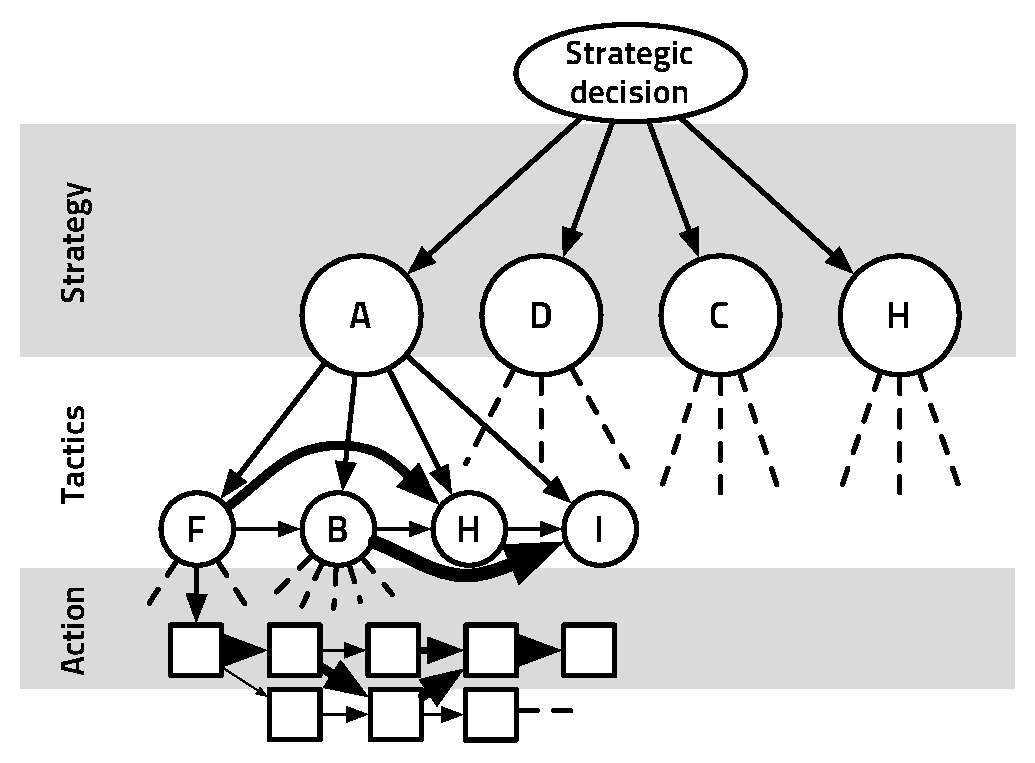
\includegraphics[width=10cm]{images/horizontal_cont_abstract_decision_hierarchy3.pdf}
\end{center}
\caption{Horizontal continuity in decision-making in a video game. The thicker the arrow, the higher the transition probability.}
\label{fig:horizontalcont}
\end{figure}

Examples? To edit, to choose with Pierre, ideas (+ point out example ``filtering out''):\\
navigation: $T^t$=go round the block, $T^{t+1}$ -> limited by future position\\
RTS: cannot switch between Front and Back attacks with the same army at close time-steps\\
simpler examples?

\subsection{Randomness}
Randomness can be inherent to the gameplay. In board games and table top role-playing, randomness often comes from throwing dice(s) to decide the outcome of actions. In decision-making theory, this induced stochasticity is dealt with in the framework of a \newacronym{mdp}{MDP}{Markov decision process}\glos{mdp}. A \gls{mdp} is a tuple of $(S,A,T,R)$ with:
\begin{itemize}
    \item $S$ a finite set of states
    \item $A$ a finite set of actions
    \item $T_a(s,s') = \PP([S^{t+1}=s']|[S^t=s],[A^t=a])$ the probability that action $a$ in state $s$ at time $t$ will lead to state $s'$ at time $t+1$
    \item $R_a(s,s')$ the immediate reward for going from state $s$ to state $s'$ with action $a$.
\end{itemize}
\gls{mdp} can be solved through dynamic programming or the Bellman value iteration algorithm \citep{Bellman}. In video games, the sheer size of $S$ and $A$ make it intractable to use \gls{mdp} directly on the whole AI task, but they are used (in research) either locally or at abstracted levels of decision. Randomness inherent to the process is one of the sources of intentional uncertainty, and we can consider player's intentions in this stochastic framework. Modeling this source of uncertainty is part of the challenge of writing game AI models.

\subsection{Partial observations}
Partial information is another source of randomness, which is found in shi-fu-mi, poker, \glos{RTS} and \glos{FPS} games, to name a few. We will not go down to the fact that the throwing of the dice seemed random because we only have partial information about its physics, or of the seed of the deterministic random generator that produced its outcome. Here, partial observations refer to the part of the game state which is deliberatively hidden between players (from a gameplay point of view): hidden hands in poker or hidden units in \glos{RTS} games due to the \glos{fogofwar}. In decision-making theory, partial observations are dealt with in the framework of a \newacronym{pomdp}{POMDP}{partially observable Markov decision process}\glos{pomdp} \citep{Sondik}. A \gls{pomdp} is a tuple $(S,A,O,T,\Omega,R)$ with $S,A,T,R$ as in a \gls{mdp} and:
\begin{itemize}
    \item $O$ a finite set of observations
    \item $\Omega$ conditional observations probabilities specifying: $\PP(O^{t+1}|S^{t+1},A^t)$
\end{itemize}
In a \gls{pomdp}, one cannot know exactly which state they are in and thus must reason with a probability distribution on $S$. $\Omega$ is used to update the distribution on $S$ (the belief) uppon taking the action $a$ and observing $o$, we have: $\PP([S^{t+1}=s']) \propto \Omega(o|s',a).\sum_{s \in S} T_a(s,s').\PP([S^t=s])$. In game AI, \gls{pomdp} are computationally intractable for most problems, and thus we need to model more carefully (without full $\Omega$ and $T$) the dynamics and the information value.
% \Omega([O^{t+1}=o]|[S^{t+1}=s'],[A^t=a])

\subsection{Time Constant(s)}

For novice to video games, we give some orders of magnitudes of the time constants involved. Indeed, we present here only real-time video games and time constants are central to comprehension of the challenges at hand. In all games, the player is taking actions continuously sampled at the minimum of the human interface device (mouse, keyboard, pad) refreshment rate and the game engine loop: at \textit{least} 30Hz. In most racing games, there is a quite high continuity in the input which is constrained by the dynamics of movements. In other games, there are big discontinuities, even if fast \glos{FPS} control resembles racing games a lot. \glos{RTS} professional gamers are giving inputs at $\approx 300$ actions per minute (\newglossaryentry{APM}{name=APM,description={action per minute, an input speed frequency in competitive gaming}}\glos{APM}).


There are also different time constants for a strategic switch to take effect. In RTS games, it may vary between the build duration of at least one building and one unit (1-2 minutes) to a lot more (5 minutes). In an RPG or a team FPS, it may even be longer (up to one full round or one game by requiring to change the composition of the team and/or the spells) or shorter by depending on the game mode. For tactical moves, we consider that the time for a decision to have effects is proportional to the mean time for a squad to go from the middle of the map (arena) to anywhere else. In RTS games, this is usually between 20 seconds to 2 minutes. Maps variability between \glos{RPG} titles and \glos{FPS} titles is high, but we can give an estimate of tactical moves to use between 10 seconds (fast FPS) to 5 minutes (some FPS, RPG).

%\subsection{Learning Curve}

\subsection{Recap}

We present the main qualitative results for big classes of gameplays (with examples) in a table page~\pageref{recapgames}.

%\begin{small}
%\setlength{\tabcolsep}{5pt}
\begin{sidewaystable}
\begin{tabular}{|l|ccccc|}
\multicolumn{6}{c}{quantization in increasing order: no, negligible, few, some, moderate, much} \\
\hline 
%Game & Combinatory & Vertical cont. & Horizontal cont. & Partial info. & Randomness & \multicolumn{3}{|c|}{Time constants} & Learning curve\\
% & & & & & & Strat. & Tact. & Act. & & \\
Game & Combinatory & Partial information & Randomness & Vertical continuity & Horizontal continuity \\
\hline
Checkers & $b\approx 4-8; d\approx 70$ & no & no & few & some \\
Chess & $b\approx 35; d\approx 80$ & no & no & some & few \\
Go & $b\approx 30-300; d\approx 150-200$ & no & no & some & moderate \\
%Monopoly 
%Battleship
Limit Poker & $b\approx 3$\footnote{fold,check,raise} $;d/hour \in [20\dots240]$\footnote{number of decisions taken per hour} & much & much & moderate & few \\
Time Racing & $b\approx 50-1,000$\footnote{$\{\ddot{x} \times \theta \times \phi\}$ sampling$\times$50Hz}$;d/min \approx 60+$ & no & no & much & much \\
(TrackMania) & & & & & \\
Team FPS & $b\approx 100-2,000$\footnote{\label{samplingFPS}$\{X \times Y \times Z\}$ sampling$\times$50Hz + firing} $;d/min \approx 100$\footnote{\label{apmFPS}60 ``continuous move actions''+ 40 (mean) fire actions per sec} & some & some & some & moderate \\
(Counter-Strike) & & & & & \\
(Team Fortress 2) & & & & & \\
FFPS duel & $b\approx 200-5,000$\ifthenelse{\equal{\myebookformat}{true}}{\footnote{$\{X \times Y \times Z\}$ sampling$\times$50Hz + firing}}{\footref{samplingFPS}} $;d/min \approx 100$\ifthenelse{\equal{\myebookformat}{true}}{\footnote{60 ``continuous move actions''+ 40 (mean) fire actions per sec}}{\footref{apmFPS}} & some & negligible & some & much \\
(Quake III) & & & & & \\
MMORPG & $b\approx 50-100$\footnote{in RPGs, there are usually more abilities than in FPS games, but the player does not have to aim to hit a target, and thus positioning plays a lesser role than in FPS.} $;d/min \approx 60$\footnote{move and use abilities/cast spells} & few & moderate & moderate & much \\
(WoW, DAoC) & & & & & \\
RTS & $b\approx 200$\footnote{atomic dir/unit $\times$ \# units + constructions + productions}$;d/min=APM\approx 300$\footnote{for pro-gamers, counting group actions as only one action} & much & negligible & moderate & some \\
(StarCraft) & & & & & \\
\hline
\end{tabular}
\label{recapgames}
\end{sidewaystable}
%\end{small}

%%%%%%%%%%%%%%%%%%%%%%%%%%%%%%%%%%%%%%%%%%%%%%%%%%%%%%%%%%%%%%%%%% 

\section{Player Characteristics}

%%% Timings, reflexes, modeling, goals, utility, backtracking, induction, ...
In all these games, knowledge and learning plays a key role. Humans compensate their lack of (conscious) computational power with pattern matching, abstract thinking and efficient memory structures. Particularly, we can classify required abilities for players to perform well in different gameplays by:
\begin{itemize}
    \item Virtuosity: the technical skill or ease of the player with given game's actions and interactions. At high level of skills, there is a strong parallel with playing a music instrument. In racing games, one has to drive precisely and react quickly. In \glos{FPS} games, players have to aim and move, while fast FPS motions resemble driving. In \glos{RPG} games, players have to use skill timely as well as have good avatar placement. Finally, in \glos{RTS} games, players have to control several units (in ``god's view''), from tens to hundreds and even sometimes thousands. They can use control groups, but it does not cancel the fact that they have to control both their economy and their armies.
    \item Deductive reasoning: the capacity to follow logical arguments, forward inference: $[A \Rightarrow B] \wedge A \Rightarrow B$. It is particularly important in Chess and Go to infer the outcomes of moves. It is important for FPS games to deduce where the enemy can be from what one has seen. In RPG games, players deduce quests solutions as well as skills/spells combinations effects. In RTS games, there is a lot of strategy and tactics that have to be infered from partial information.
    \item Inductive reasoning: the capacity for abstraction, generalization, going from simple observations to a more general concept. A simple example of generalization is: $[Q$ of the sample has attribute $A] \Rightarrow [Q$ of the population has attribute $A]$. In all games, it is important to be able to induce the overall strategy of the opponent's from action-level observations. In games which benefit from a really abstract level of reasoning (Chess, Go, RTS), it is particularly important as it allows to reduce the complexity of the problem at hand, by abstracting it and reasoning in abstractions.
    \item Decision-making: the capacity to take decisions, possibly under uncertainty and stress. Selecting a course of actions to follow while not being sure of their effect is a key ability in games, particularly in (very) partial information games as Poker (in which randomness even adds to the problem) and RTS games. It is important in Chess and Go too as reasoning about abstractions (as for RTS) brings some uncertainty about the effects of moves too.
    \item Knowledge: we distinguish two kinds of knowledge in games: knowledge of the game and knowledge of particular situations (``knowledge of the map''). The duality doesn't exist in Chess, Go and Poker. However, for instance for racing games, knowledge of the map is most often more important than knowledge of the game (game mechanics and game rules, which are quite simple). In FPS games, this is true too as good shortcuts, ambushes and efficient movements comes from good knowledge of the map, while rules are quite simple. In RPG, rules (skills and spells effects, durations, costs...) are much more complex to grasp, so knowlege of the game is perhaps more important. Finally, for RTS games, there are some map-specific strategies and tactics, but the game rules and overall strategies are also already complex to grasp. The longer are the rules of the game to explain, the higher the complexity of the game and thus the benefit from knowledge of the game itself.
    \item Psychology: the capacity to know the opponent's move by knowing them, their style, and reasoning about what they think. It is particularly important in competitive games for which there are multiple possible styles, which is not really the case for Chess, Go and racing games. As players have multiple possible valid moves, reasoning about their decision-making process and effectively predicting what they will do is what differentiate good players from the best ones.
\end{itemize}

Finally, we made a quick survey among gamers and regrouped the 108 answers in table~\ref{surveygamers} page~\pageref{surveygamers}. The goal was a to get a grasp on which skills are correlated to which gameplays. The questions that we asked can be found in Appendix~\ref{apdx:survey}. Answers mostly come from good to highly competitive (on a national level) amateurs. To test the ``psychology'' component of the gameplay, we asked players if they could predict the next moves of their opponents by knowing them personally or by knowing what the best moves (best play) was for them. As expected, Poker has the strongest psychological dimension, followed by FPS and RTS games.
\\

%\subsection{Virtuosity} skill
%\subsection{Deduction}
%\subsection{Induction}
%\subsection{Decision-Making}
%\subsection{Psychology}
%\subsection{Recap}

%%% https://en.wikipedia.org/wiki/Cognition
%%% \begin{sidewaystable}
%%% \begin{tabular}{|l|ccccccc|}
%%% \hline 
%%% Game & Virtuosity & Deduction & Induction & Decision-Making & \multicolumn{3}{c|}{Knowledge} \\
%%%      & (sensory-motor) & (analysis) & (abstraction) & (acting) & game & map & opponent \\
%%% Checkers &   & ++ & &   & ++& &+ \\
%%% Chess &   & ++ & &   & ++& &+ \\
%%% Go &   & ++ & + &   & ++& &+ \\
%%% Limit Poker &   & + & + & ++ & ++& &++ \\
%%% Time Racing & ++ &   &   &   & +&++&  \\
%%% (TrackMania) & & & & & & & \\
%%% Team FPS & & & & & & & \\ 
%%% (Counter-Strike) & & & & & & & \\ 
%%% (Team Fortress 2) & & & & & & & \\ 
%%% FFPS duel & ++ & + &   & + & +&++&+ \\
%%% (Quake III) & & & & & & & \\ 
%%% MMORPG & + & + & + & ++ & +&++&+ \\
%%% (WoW, DAoC) & & & & & & & \\ 
%%% RTS & ++ & ++ & ++ & ++ & ++&+&++ \\
%%% (StarCraft) & & & & & & & \\
%%% \hline
%%% \end{tabular}
%%% \end{sidewaystable}

\begin{sidewaystable}

\begin{tabular}{|l|cccccc|}                                                     
\hline                                                                          
Game & Virtuosity\footnote{``skill'', dexterity of the player related to the game, as for a musician with their instrument.} & Deduction \footnote{capacity for deductive reasoning; from general principle to a specific conclusion.} & Induction \footnote{capacity for inductive reasoning, abstraction, generalization; from specific examples to a general conclusion.} & Decision-Making\footnote{capacity to select a course of actions in the presence of several alternatives, possibly under uncertainty and stress.} & Opponent prediction\footnote{what is the biggest indicator to predict the opponent's moves: their psychology (subjective) or the rules and logic of the game (objective)?} & Advantageous knowledge\footnote{Is knowledge of the game in general, or of the map specifically, preferable in order to play well?} \\
 & (sensory-motor) & (analysis) & (abstraction) & (taking action) & -1: subjectivity & -1: map \\
 & [0-2] & [0-2] & [0-2] & [0-2] & 1: objectivity & 1: game \\
\hline                                                                     
Chess (n: 35) &  X  & 1.794 & 1.486 & 1.657 & 0.371 &  X  \\                
Go (n: 16) &  X  & 1.688 & 1.625 & 1.625 & 0.562 &  X  \\                   
Poker (n: 22) &  X  & 1.136 & 1.591 & 1.545 & -0.318 &  X  \\               
Racing (n: 19) & 1.842 & 0.263 & 0.211 & 1.000 & 0.500 & -0.316 \\         
Team FPS (n: 40) & 1.700 & 1.026 & 1.075 & 1.256 & 0.150 & -0.105 \\     
Fast FPS (n: 22) & 2.000 & 1.095 & 1.095 & 1.190 & 0.000 & 0.150 \\           
MMORPG (n: 29) & 1.069 & 1.069 & 1.103 & 1.241 & 0.379 & 0.759 \\           
RTS (n: 86) & 1.791 & 1.849 & 1.687 & 1.814 & 0.221 & 0.453 \\           
\hline
\end{tabular}
\label{surveygamers}
\end{sidewaystable}

%%%%%%%%%%%%%%%%%%%%%%%%%%%%%%%%%%%%%%%%%%%%%%%%%%%%%%%%%%%%%%%%%% 

%%% \section{An interesting problem}
%%% \subsection{Simulated but stochastic}
%%% Human players (ally or foes), and sometimes (most of the time) stochasticity in the rules of the game (fog of war, randomness, etc.).

\chapter{Bayesian Modeling of Multi-player Games}

%%% Nothing in Nature is random. ... A thing appears random only through the incompleteness of our knowledge.
%%% - Benedict Spinoza -

\begin{quotation}
\noindent
\textit{On voit, par cet Essai, que la théorie des probabilités n'est, au fond, que le bon sens réduit au calcul; elle fait apprécier avec exactitude ce que les esprits justes sentent par une sorte d'instinct, sans qu'ils puissent souvent s'en rendre compte.
\vspace{0.2cm} \\
One sees, from this Essay, that the theory of probabilities is basically just common sense reduced to calculus; it makes one appreciate with exactness that which accurate minds feel with a sort of instinct, often without being able to account for it.}
%\vspace{0.2cm} \\
\begin{flushright}Pierre-Simon de Laplace (Essai philosophique sur les probabilit\'{e}s, 1814)\end{flushright}\end{quotation}
%\begin{flushright}Pierre-Simon de Laplace (1814)\end{flushright}\end{quotation}

%%% \begin{quotation}
%%% The actual science of logic is conversant at present only with things either certain, impossible, or entirely doubtful, none of which (fortunately) we have to reason on. Therefore the true logic for this world is the calculus of Probabilities, which takes account of the magnitude of the probability which is, or ought to be, in a reasonable man's mind.
%%% \begin{flushright}James Clerk Maxwell (Letter to Lewis Campbell, 1850)\end{flushright}\end{quotation}


\lettrine{H}{ere}, we now present the use of probability theory as an alternative to logic, transforming incompleteness into uncertainty. Bayesian models can deal with both intentional and extensional uncertainty, that is: uncertainty coming from intentions of the players or the stochasticity of the game, as well as uncertainty coming from imperfect information and the model's limits. We will first show how these problems are addressed by probabilities and how to structure a full Bayesian program. We illustrate the approach with a model evaluated on a simulated \glos{MMORPG} situation.

\ifthenelse{\equal{\myebookformat}{false}}{
\chaptertoc
}{}

%Bot AI has to be adaptive, robust, multi-scale.
%Why?
%\begin{itemize}
%\item The bot can't cheat (at least it's not fun!)
%\item The bot can't assume optimal play from the opponent when the problem is so large
%\item The bot can learn from others games, self past games, self current game
%\item The bot can't be in the head of your opponent (meta-)
%\end{itemize}

\section{Problems in Game AI}
We sum up the problems that we have detailed in the previous chapter to make a good case for a consistent reasoning scheme which can deal with uncertainty.

\subsection{Partial information}
If the AI has perfect information, behaving realistically is the problem. Cheating bots are not fun, so either AI should just use information available to the players, or it should fake having only partial information. In probabilistic modeling, sensor models allow for the computation of the state $S$ from observations $O$ by asking $\PP(S|O)$. One can easily specify or learn $\PP(O|S)$: either the game designers specify it, or the bot uses perfect information to get $S$ and learns (counts) $\PP(O|S)$, then infer $\PP(S|O) = \frac{\PP(O|S).\PP(S)}{\PP(O)}$ (Bayes rule). Incompleteness of information is just uncertainty about the full state.

\subsection{Randomness}
Some games have inherent stochasticity (variable random action effects) part of the gameplay. In any case, an AI can't assume optimal play from the opponent due to the complexity of video games. In the context of state estimation and control, dealing with this randomness require ad-hoc methods for scripting of boolean logic, while it is dealt with natively through probabilistic modeling. Where a program would have to test for an effect/value $V$ to be in a given interval to decide on a given course of action $A$, a probabilistic model just computes the distribution on $A$ given $V$: $\PP(A|V) = \frac{\PP(V|A).\PP(A)}{\PP(V)}$.

\subsection{Vertical continuity}
Abstracting higher level cognitive functions (strategy and tactics for instance) is an efficient way to break the complexity barrier of writing game AI. Exploiting the vertical continuity, i.e. the conditioning of higher level thinking on actions, is totally possible in a hierarchical Bayesian model. With strategies as values of $S$ and tactics as values of $T$, $\PP(T|S)$ gives the conditioning of $T$ on $S$ and thus enables us to evaluate only those $T$ values that are possible with given $S$ values.

\subsection{Horizontal continuity}
Real-time games may use discrete time-steps (24Hz for instance for StarCraft), it does not prevent temporal continuity in strategies, tactics and, most strongly, actions. There are several Bayesian models able to deal with sequences, filter models, from which \newglossaryentry{HMM}{name=HMM,description={Hidden Markov Model, a dynamic Bayesian network estimating hidden states following a Markov process from observations}}Hidden Markov Models (\glos{HMM}) \citep{Rabiner}, Kalman filters \citep{Kalman1960} and particle filters \citep{particleFiltering} are specializations of. With states $S$ and observations $O$, filter models under the Markov assumption represent the joint $\PP(S^0).\PP(O^0|S^0).\prod_{t=1}^T[\PP(S^t | S^{t-1}).\PP(O^t|S^t)]$.

\subsection{Autonomy and Programming}
Autonomy is the ability to deal with new states: the challenge of autonomous characters arises from state spaces too big to be fully specified (in scripts / FSM). Again, probabilistic modeling enables one to recognize unspecified states as soft mixtures of known states. It also allows to deal with unknown state as an incomplete version of a known state which subsumes it. Autonomy can also be reached through learning, being it through online or offline learning. Offline learning is used to learn parameters that does not have to be specified by the programmers and/or game designers. One can use data or experiments with known/wanted situations (supervised learning, reinforcement learning), or explore data (unsupervised learning) or game states (evolutionary algorithms). Online learning can provide adaptability of the AI to the player and/or its own competency playing the game.

\section{The Bayesian Programming Methodology}

\subsection{The Hitchhiker's Guide to Bayesian Probability}
\begin{figure}[h]
\centering
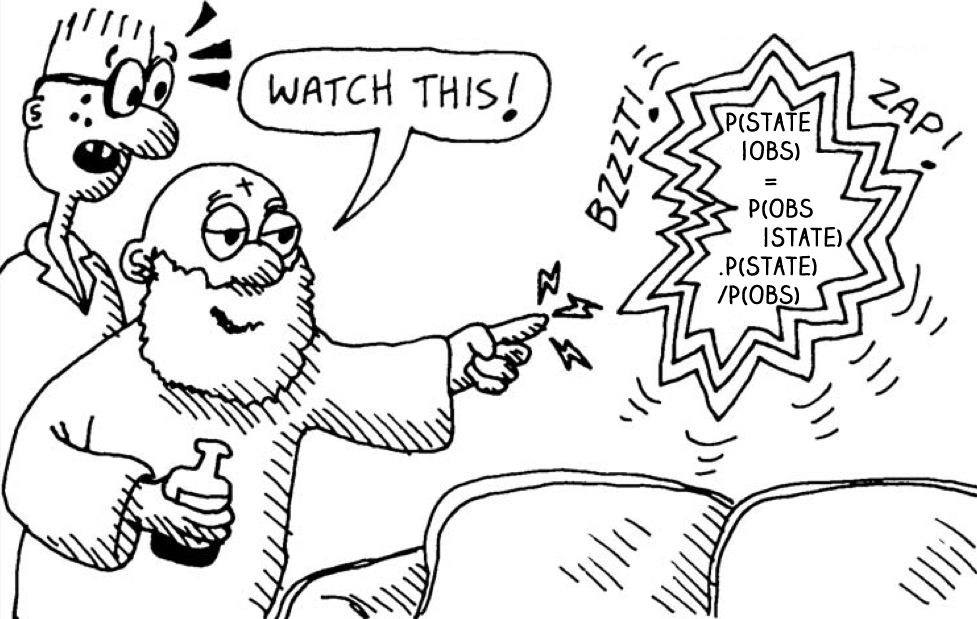
\includegraphics[width=8cm]{images/zapBayes3.png}
\caption{An advisor introducing his student to Bayesian modeling, adapted from \underline{Land of Lisp} with the kind permission of \cite{LoL}.}
%\footnote{\copyright Conrad Barski, in \underline{Land of Lisp}, ed. No Starch Press, \url{http://landoflisp.com/}}
\end{figure}


The reverend Thomas Bayes is the first credited to have worked on inversing probabilities: by knowing something about the probability of $A$ given $B$, how can one draw conclusions on the probability of $B$ given $A$? Bayes theorem states: $$\PP(A|B) = \frac{\PP(B|A)\PP(A)}{\PP(B)}$$
\cite{Laplace} rediscovered this theorem and published the work of inductive reasoning by using probabilities. Later, by extending logic to \textit{plausible reasoning}, \cite{Jaynes} arrived at the same properties than \cite{Kolmogorov33} probability theory. Plausible reasoning originates from logic, whose statements have degrees of plausibility represented by real numbers. %We note ``the conditional plausibility that A is true, given that B is true'' $A|B$.
Adding consistency: a) all the possible ways to reach a conclusion leads to the same result, b) information cannot be ignored, c) two equal states of knowledge have the same plausibilities; Cox %%% Jaynes too
derived the ``product-rule'' ($\PP(A,B)=\PP(A\cap B)=\PP(A|B)\PP(B)$) and the ``sum-rule'' ($\PP(A+B)=\PP(A)+\PP(B)-\PP(A,B)$ or $\PP(A\cup B) = \PP(A)+\PP(B)-\PP(A\cap B)$) of probabilities. As for rules of inferences, the links between logic and plausible reasoning are direct, with $C=[A\Rightarrow B]$:
\begin{itemize}
    \item modus ponens $$\frac{[A\Rightarrow B] \wedge [A=true]}{B=true}$$ translates to $$\PP(B|A,C)=\frac{\PP(A,B|C)}{\PP(A|C)}$$
    \item modus tollens $$\frac{[A\Rightarrow B] \wedge [B=false]}{A=false}$$ translates to $$\PP(A|C\neg B)=\frac{\PP(A \neg B|C)}{\PP(\neg B|C)}$$
\end{itemize}
Also, additionally to the two strong logic syllogisms above, plausible reasoning gets two weak syllogisms, from:
\begin{itemize}
    \item $$\PP(A|B,C)=\PP(A|C)\frac{\PP(B|A,C)}{\PP(B|C)}$$ we get $$\frac{[A\Rightarrow B] \wedge [B=true]}{A\ \mathrm{becomes\ more\ plausible}}$$
    \item $$\PP(B| C\neg A)=\PP(B|C)\frac{\PP(\neg A|B,C)}{\PP(\neg A|C)}$$ we get $$\frac{[A\Rightarrow B] \wedge [A=false]}{B\ \mathrm{becomes\ less\ plausible}}$$
\end{itemize}

Indeed, this was proved by \cite{Cox46}, producing Cox's theorem (also named Cox-Jayne's theorem):
\begin{mythm}
A system for reasoning which satisfies:
\begin{itemize}
    \item divisibility and comparability, the plausibility of a statement is a real number,
    \item common sense, in presence of total information, reasoning is isomorphic to Boolean logic,
    \item consistency, two identical mental states should have the same degrees of plausibility,
\end{itemize}
is isomorphic to probability theory.
\end{mythm}
So, the degrees of belief, of any consistent induction mechanism, verify Kolmogorov's axioms. \cite{DeFinetti37} showed that if reasoning is made in a system which is not isomorphic to probability theory, then it is always possible to find a \textit{Dutch book} (a set of bets which guarantees a profit regardless of the outcomes). \textbf{In our quest for a consistent reasoning mechanism which is able to deal with (extensional and intentional) uncertainty, we are thus bound to probability theory.} %%% ``Probability does not exist''


\subsection{A Formalism for Bayesian Models}
Inspired by plausible reasoning, we present Bayesian programming, a formalism that can be used to describe entirely any kind of Bayesian model. It subsumes Bayesian networks and Bayesian maps, as it is equivalent to probabilistic factor graphs \cite{Diard03}. There are mainly two parts in a \newacronym{BP}{BP}{Bayesian program}\glos{BP}, the \textbf{description} of how to compute the joint distribution, and the \textbf{question(s)} that it will be asked. 

The description consists in exhibiting the relevant \textit{variables} $\{X^1,\dots,X^n\}$ and explain their dependencies by \textit{decomposing} the joint distribution $\PP(X^1\dots X^n | \delta, \pi)$ with existing preliminary (\textit{prior}) knowledge $\pi$ and data $\delta$. The \textit{forms} of each term of the product specify how to compute their distributions: either parametric forms (laws or probability tables, with free parameters that can be learned from data $\delta$) or recursive questions to other Bayesian programs.

Answering a question is computing the distribution $\PP(Searched | Known)$, with $Searched$ and $Known$ two disjoint subsets of the variables. 
%%%$P(Searched | Known) = \begin{small} \frac{\sum_{Free}P(Searched\ Free\ Known)}{P(Known)} \end{small} = \frac{1}{Z}\times \sum_{Free} P(Searched\ Free\ Known)$. 
\begin{eqnarray}
& & \PP(Searched | Known) \\
& = & \frac{\sum_{Free}\PP(Searched,\ Free,\ Known)}{\PP(Known)} \\
& = & \frac{1}{Z}\times \sum_{Free} \PP(Searched,\ Free,\ Known)
\end{eqnarray}

General Bayesian inference is practically intractable, but conditional independence hypotheses and constraints (stated in the description) often simplify the model. There are efficient ways to calculate the joint distribution like message passing and junction tree algorithms \citep{Pearl,AjiM00,Nai04,mekhnacha,Koller}. Also, there are different well-known approximation techniques: either by sampling with Monte-Carlo (and Monte-Carlo Markov Chains) methods \citep{MacKay,Andrieu}, or by calculating on a simpler (tractable) model which approximate the full joint as with variational Bayes \citep{Beal}.

%\begin{small}
\begin{eqnarray*}
%\begin{sideways}\parbox{35mm}{\hspace{-1.3cm}Bayesian program}\end{sideways}
BP
\begin{cases}
%\begin{sideways}\parbox{15mm}{\hspace{-0.8cm}Description}\end{sideways}
Desc.
\begin{cases}
%\begin{sideways}\parbox{35mm}{\hspace{-1.1cm}Specification ($\pi$)}\end{sideways}
Specif. (\pi)
\begin{cases}
Variables\\
Decomposition\\
Forms\ (Parametric\ or\ Program)\\
\end{cases}\\
Identification\ (based\ on\ \delta)\\
\end{cases}\\
Question
\end{cases}
\end{eqnarray*}
%\end{small}


For the use of Bayesian programming in sensory-motor systems, see \citep{PRDMSMS}. For its use in cognitive modeling, see \citep{Colas10}. For its first use in video game AI, applied to the first person shooter gameplay (Unreal Tournament), see \citep{LeHy04}.

To sum-up, by viewing probabilities as an extension of logic, the method by which to build Bayesian models gets clearer: there is a strong parallel between writing a Bayesian program and logic or declarative programming. In order:
\begin{enumerate}
    \item Isolate the variables of the problem: it is the first prior that the programmer puts into the system. The variables can be anything, from existing input or output values of the problem to abstract/aggregative values or parameters of the model. Discovering which variable to use for a given problem is one of the most complicated form of machine learning.
    \item Suppose and describe the influences and dependencies between these variables. This is another prior that the programmer can have on the problem, and learning the structure between these variables is the second most complicated form of learning \citep{Fra04b,Ler05a}.
    \item Fill the priors and conditional probabilities parameters. The programmer needs to be an expert of the problem to put relevant parameters, although this is the easiest to learn from data once variables and structure are specified. Learning the structure can be seen as learning the parameters of a fully connected model and then removing dependencies where are the less influent parameters.% but most of these kinds of model are totally intractable.
\end{enumerate}
In the following, we present how we applied this method to a simulated \glos{MMORPG} fight situation as an example.

By following these steps, one may have to choose among several models. That is not a problem as there are rational ground to make this choices, ``all models are wrong; some are useful'' (George Box). %We express this choice of modeling in $\pi$. 
Actually, the full question that we ask is $\PP(Searched|Known, \pi, \delta)$, it depends on the modeling assumptions ($\pi$) as well as the data ($\delta$) that we used for training (if any). A simple way to view model selection is to pick the model which makes the fewest assumptions (Occam's razor). In fact, Bayesian inference carries Occam's razor with it: we shall ask what is the plausibility of our model prior knowledge in the light of the data $\PP(\pi|\delta)$. 

Indeed, when evaluating two models $\pi_1$ and $\pi_2$, doing the ratio of evidences for the two modeling assumption helps us choose:
\begin{equation}
\frac{\PP(\pi_1 | \delta)}{\PP(\pi_2 | \delta)} = \frac{\PP(\pi_1) \PP(\delta| \pi_1)}{\PP(\pi_2 | \delta) \PP(\delta | \pi_2)}
\end{equation}

If our model is complicated, its expressiveness is higher, and so it can model more complicated datasets. However, the probability mass will be spread thiner on the space of possible datasets than for a simpler model. For instance, in the task of regression, if $\pi_1$ can only encode linear regression ($y = Ax + b$) and $\pi_2$ can also encore quadratic regression ($y = Ax + Bx^2 + c$), all the predictions for $\pi_1$ are concentrated on linear (affine) functions, while for $\pi_2$ the probability mass of predictions is spread on more possible functions. If we only have data $\delta$ of linear functions, the evidence for $\pi_1$, $\PP(\pi_1|\delta)$ will be higher. If $\delta$ contains some quadratic functions, the evidence ratio will shift towards $\pi_2$ as the second model has better predictions: the shift to $\pi_2$ happens when the additional model complexity of $\pi_2$ and the prediction errors of $\pi_1$ balance each other.


%%% How?
%%% \begin{itemize}
%%% \item Bayesian programming methodology
%%% \item When in doubt, toss the distribution to your neighbour
%%% \item Exploit gameplay/game rules structure
%%% \item Learn and eat data for breakfast
%%% \item Meta- can be solved by being (globally) stateless and applying the same model as self on the opponent with her sensory inputs
%%% \end{itemize}

\section{Modeling of a Bayesian MMORPG player}
\subsection{Task}

We will now present a model of a \glos{MMORPG} player with the Bayesian programming framework \citep{SYNNAEVE:MMORPG}. A role-playing game (RPG) consist in the incarnation by the human player of an avatar with specific skills, items, numbers of health points (HP) and stamina or mana (magic energy) points (we already presented this gameplay in section~\ref{sec:MMORPG}). We want to program a robotic player which we can substitute to a human player in a battle scenario. More specifically here, we modeled the ``druid'' class, which is complex because it can cast spells to deal damages or other negative effects as well as to heal allies or enhance their capacities (``buff'' them). The model described here deals only with a sub-task of a global AI for autonomous NPC. 

The problem that we try to solve is: how do we choose which skill to use, and on which target, in a \glos{PvE} battle? The possible targets are all our allies and foes. There are also several skills that we can use. We will elaborate a model taking all our perceptions into account and giving back a distribution over possible target and skills. We can then pick the most probable combination that is yet possible to achieve (enough energy/mana, no cooldown/reload time) or simply sample in this distribution. %For that, we first choose what should be the target given all surrounding variables: is an ally near death that he should be healed, which foe should we focus our attacks on? Once we have the distribution over possible targets, we search the distribution about our skills, pondered by the one on targets. However, some variables can be things that humans subconsciously interpolate from perceptions.

An example of the tasks that we have to solve is depicted in Figure~\ref{fig:wow_fight}): red characters are foes, green ones are allies, we control the blue one. The ``Lich'' is inflicting damages to the ``MT'' (main tank), the ``Add'' is hitting the ``Tank''. In setup A, only the ``Tank'' is near death, while in setup B both the ``Tank'' and the ``Add'' are almost dead. A first approach to reason about these kind of situations would be to use the combination of simple rules and try to give them some priority.
\begin{itemize}
    \item if an ally has less than \textit{X} (threshold) HP then use a ``heal'' on him.
    \item if the enemy receiving most damage has resistances (possibly in a list), lower them if possible.
    \item if allies (possibly in a list) are not ``buffed'' (enhanced), buff them if possible.
    \item default: shoot at the most targeted enemy.
    \item self-preservation, etc.
\end{itemize}
The problem with such an approach is that tuning or modifying it can quickly be cumbersome. Also, the behavior would seem pretty repetitive and robustness is not ensured.

\begin{figure}[h!]
\begin{center}
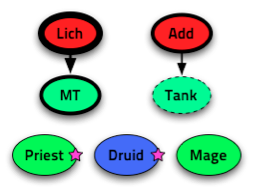
\includegraphics[width=5cm]{images/wow_fight1.png} \hspace{1.5cm} 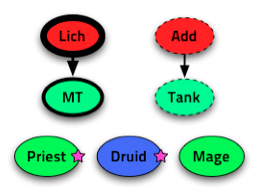
\includegraphics[width=5cm]{images/wow_fight2.png}
\caption{Example setup A (left) and B (right). There are 2 foes and 2 allies taking damages (``MT'' and ``tank''). Players with stars can heal allies, players with dotted lines will soon die ($ID=true$). Our model controls the blue character, green players are allies, while red characters are foes. The larger the surrounding ellipse is, the more health points the characters have.}
\label{fig:wow_fight}
\end{center}
\end{figure}

\subsection{Perceptions and actions}
We now list some of the perceptions available to the player (and thus the robot):
\begin{itemize}
    \item the names and positions of all other players, this gives their distances, which is useful to know which abilities can be used.
    \item hit points (also health points, noted HP) of all the players, when the HP of a player fall to 0, her avatar dies. It can be resurrected, but not during the fight, at least in the situations that we consider.
    \item the natures of other players (ally or foe).
    \item the class of other players: some have a tanking role (take incoming damages for the rest of the group), others are damage dealers (either by contact or ranged attacks), the last category are healers, whose role is to maintain everyone alive.
    \item an approximation of the resistance to certain types of attacks for every player.
\end{itemize}

Actions available to the players are to move and to use their abilities:
\begin{itemize}
    \item damage over time attacks (periodic repeated damage), or quick but low damage attacks, and slow but high damage attacks
    \item energy/mana/stamina regenerators
    \item heal over time (periodic heal to selected allies), or quick but small heals, and slow but big heals
    \item immobilizations, disabling effects (``stun'')
    \item enhancement of the selected allies HP/attack/speed... and crippling attacks (enhancing future attacks), maledictions
    \item removing maledictions...
\end{itemize}

Here, we consider that the choice of a target and an ability to use on it strongly condition the movements of the player, so we will not deal with moving the character.

\subsection{Bayesian model}
\subsubsection{Variables}

A simple set of variables is as follows: 
\begin{itemize}
    \item Target: $T^{t-1,t} \in \{t_1\dots t_n\}$ at $t$ and $t-1$ (previous action). $T^t$ is also abusively noted $T$ in the rest of the model. We have the $n$ characters as possible targets; each of them has their own properties variables (the subscripting in the following variables). 
    %\item Hit Points: $HP_1 \dots HP_n$ s.t. $HP_i \in [0\dots 9]$. Health/Hit points ($HP$) are discretized in 10 levels, from the lower to the higher. 
    \item Hit Points: $HP_{i \in \llbracket 1\dots n\rrbracket} \in [0\dots 9]$ is the hit points value of the $i$th player. Health/Hit points ($HP$) are discretized in 10 levels, from the lower to the higher. 
    %\item Distance: $D_1 \dots D_n$ s.t. $D_i \in \{Contact, Close, Far, VeryFar\}$. Distance ($D$) is discretized in 4 zones around the robot character: \textit{contact} where it can attack with a contact weapon, \textit{close}, \textit{far} and (\textit{very far}) to the further for which we have to move even for shooting the longest distance weapon/spell. 
    \item Distance: $D_{i \in \llbracket 1 \dots n \rrbracket} \in \{Contact, Close, Far, VeryFar\}$ is the distance of the $i$th player to our robotic character. Distance ($D$) is discretized in 4 zones around the robot character: \textit{contact} where it can attack with a contact weapon, \textit{close}, \textit{far} and (\textit{very far}) to the further for which we have to move even for shooting the longest distance weapon/spell. 
    %\item Ally: $A_1 \dots A_n$ s.t. $A_i \in \{true, false\}$. Ally ($A$) is a Boolean variable mentioning if character $i$ is allied with the robot character. 
    \item Ally: $A_{i \in \llbracket 1 \dots n \rrbracket} \in \{true, false\}$ is $true$ is the $i$th player is an ally, and false otherwise.
    %\item Derivative Hit Points: $\Delta HP_1 \dots \Delta HP_n$ s.t. $\Delta HP_i \in \{-, 0, +\}$. Delta hit points ($\Delta HP$) is a 3-valued interpolated value from the previous few seconds of fight that informs about the $i$th character getting wounded or healed (or nothing). 
    \item Derivative Hit Points: $\Delta HP_{i \in \llbracket 1 \dots n \rrbracket} \in \{-, 0, +\}$ (decreasing, stable, increasing) is the evolution of the hit points of the $i$th player. $\Delta HP$ is a 3-valued interpolated value from the previous few seconds of fight that informs about the $i$th character getting wounded or healed (or nothing). 
    %\item Imminent Death: $ID_1 \dots ID_n$ s.t. $ID_i \in \{true, false\}$. Imminent death ($ID$) is also an interpolated value that encodes $HP$, $\Delta HP$ and incoming attacks/attackers. This is a Boolean variable saying if the $i$th character if going to die anytime soon. This is an example of what we consider that an experienced human player will infer automatically from the screen and notifications. 
    \item Imminent Death: $ID_{i \in \llbracket 1 \dots n \rrbracket} \in \{true, false\}$ tells if the $i$th player is in danger of death. Imminent death ($ID$) is an interpolated value that encodes $HP$, $\Delta HP$ and incoming attacks/attackers. %
This is a Boolean variable saying if the $i$th character if going to die anytime soon. This is an example of what we consider that an experienced human player will infer automatically from the screen and notifications. 
    \item Class: $C_{i \in \llbracket 1 \dots n} \in \{Tank, Contact, Ranged, Healer\}$ is the class of the $i$th player. Class ($C$) is simplified over 4 values: a Tank can take a lot of damages and taunt enemies, a Contact class which can deal huge amounts of damage with contact weapons (rogue, barbarian...), Ranged stands for the class that deals damages from far away (hunters, mages...) and Healers are classes that can heal in considerable amounts. 
    %\item Class: $C_{i \in \llbracket 1 \dots n} \in \{Tank, Contact, Ranged, Healer\}$ is the class of the $i$th player. Class ($C$) is simplified over 4 values: a Tank can take a lot of damages and taunt enemies, a Contact class which can deal huge amounts of damage with contact weapons (rogue, barbarian...), Ranged stands for the class that deals damages from far away (hunters, mages...) and Healers are classes that can heal in considerable amounts. 
    \item Resists: $R_{i \in \llbracket 1 \dots n \rrbracket} \in \{Nothing, Fire, Ice, Nature, FireIce, IceNat, FireNat, All\}$ informs about the resistances of the $i$th player. The Resist variable is the combination of binary variables of resistance to certain types of (magical) damages into one variable. With 3 possible resistances we get ($2^3$) 8 possible values. For instance ``$R_i=FireNat$'' means that the $i$th character resists fire and nature-based damages. Armor (physical damages) could have been included, and the variables could have been separated. 
    \item Skill: $S \in \{Skill_1 \dots Skill_m\}$. The skill variable takes all the possible skills for the given character, and not only the available ones to cast at the moment to be able to have reusable probability tables (i.e. it is invariant of the dynamics of the game).
\end{itemize}

\subsubsection{Decomposition}

%\subsubsection{Target selection}
%%% The joint distribution is simplified (by conditional independence of variables) as:
%%% \begin{eqnarray}
%%% \PP(T, T^{t-1}, HP_{1:n}, D_{1:n}, A_{1:n}, \Delta HP_{1:n}, ID_{1:n}, C_{1:n}) = \\
%%% \PP(T^{t-1}).\PP(T|T^{t-1}).\prod_{i=1}^n [ \PP(HP_i | A_i, C_i, T).\PP(D_i | A_i, t).\PP(A_i | T)\\
%%% \PP(\Delta HP_i | A_i, C_i, T).\PP(C_i | A_i, T).\PP(ID_i | T) ]
%%% \end{eqnarray}
%%% We want to compute the probability distribution on the variable Target ($T$), so we have to consider the joint distribution with all variables on which Target ($T$) is conditionally dependant : the previous value of Target ($T^{t-1}$), and all the variables on each character (except for Resists). The probability of a given target depends on the previous one (it encodes the previous decision and so all previous states). The health (or hit) points ($HP_i$) depends on the facts that the $i$th character is an ally ($A_i$), on his class ($C_i$), and if he is a target ($T$). Such a conditional probability table should be learned, but we can already foresee that a targeted ally with a tanking class ($C=tank$) would have a high probability of having low hit points ($HP$) because taking it for target means that we intend to heal him. The distance of the unit $i$ ($D_i$) is more probably far if unit $i$ is an enemy ($A_i=false$) and we target it ($T=i$) as our kind of druid attacks with ranged spells and does not fare well in the middle of the battlefield. The probability of the $i$th character being an ally depends on if we target allies of foes more often: that is $\PP(A_i|T)$ encodes our propensity to target allies (with heals and enhancements) or foes (with damaging or crippling abilities). The probability that the $i$th units is being damaged (losing hit points: $\Delta HP_i=``-''$) is higher for foes ($A_i=false$) with vulnerable classes ($C_i=healer$) that are more succeptible to be targeted ($T=i$), and also for allies ($A_i=true$) whose role is to take most of the damages ($C_i=tank$). As for $A_i$, the probability of $ID_i$ is driven by our %soft evidence 
%%% inclination of targeting characters near death. The probability of $C_i$ is driven by the distribution of foes and allies population, tuned with a soft evidence of which classes our druid human player will target more frequently. %Each and every time, if $T \neq i$, the probability of the left variable is given according to the uniform distribution. For the task of computing the distribution on Target, the joint distribution is simplified (by conditional independence of variables) as:


%\subsubsection{Skill selection}
The joint distribution of the model is: 
\begin{eqnarray}
\PP(S, T^{t-1,t}, HP_{1:n}, D_{1:n}, A_{1:n}, \Delta HP_{1:n}, ID_{1:n}, C_{1:n}, R_{1:n}) = \\
\PP(S).\PP(T^t|T^{t-1}).\PP(T^{t-1}).\prod_{i=1}^n \big[ \PP(HP_i | A_i, C_i, S, T).\PP(D_i | A_i, S, T).\PP(A_i | S, T) \\
        \PP(\Delta HP_i | A_i, S, T). \PP(R_i | C_i, S, T). \PP(C_i | A_i, S, T) \PP(ID_i | T)\big]
\end{eqnarray}
We want to compute the probability distribution on the variable target ($T$) and skill ($S$), so we have to consider the joint distribution with all variables on which target ($T$) or skill ($S$) are conditionally dependent: the previous value of target ($T^{t-1}$), and all the perceptions variables on each character. 

\begin{itemize}
    \item The probability of a given target depends on the previous one (it encodes the previous decision and so all previous states). 
    \item The health (or hit) points ($HP_i$) depends on the facts that the $i$th character is an ally ($A_i$), on his class ($C_i$), and if he is a target ($T$). Such a conditional probability table should be learned, but we can already foresee that a targeted ally with a tanking class ($C=tank$) would have a high probability of having low hit points ($HP$) because taking it for target means that we intend to heal him.
    \item The distance of the unit $i$ ($D_i$) is more probably far if unit $i$ is an enemy ($A_i=false$) and we target it ($T=i$) as our kind of druid attacks with ranged spells and does not fare well in the middle of the battlefield.
    \item The probability of the $i$th character being an ally depends on if we target allies of foes more often: that is $\PP(A_i|T)$ encodes our propensity to target allies (with heals and enhancements) or foes (with damaging or crippling abilities).
    \item The probability that the $i$th units is losing hit points ($\Delta HP_i=minus$) is higher for foes ($A_i=false$) with vulnerable classes ($C_i=healer$) that are more succeptible to be targeted ($T=i$), and also for allies ($A_i=true$) whose role is to take most of the damages ($C_i=tank$). As for $A_i$, the probability of $ID_i$ is driven by our %
||
. The probability that the $i$th units is being damaged ($\Delta HP_i=``-''$) will top when we use a heal ($S=heal$) on an ally, as we want to maintain everyone alive.  
    \item Obviously, the usage of skills depends on their efficiency on the target ($R$, resistances), and on their class. As a result, we have $\PP(R_i|C_i,S,T)$ as the conditional distribution on ``resists''. The probability of the resist to ``nature based effects'' ($R_i=nature$) for skills involving ``nature'' damage ($s \in \{nature\_damage\}$) will be very low as it will be useless to use spells that the receiver is protected against.
    \item The probability that the $i$th character will die soon ($ID_i$) will be high if $i$ is targeted ($T=i$) with a big heal or big instant damage ($S=big\_heal$ or $S=big\_damage$, depending on whether $i$ is an ally or not). 

\end{itemize}
% As previously for targets, we are interested in the conditional probabilities of each character's state variables given other state variables and given our target ($T$) and the skill that we use ($S$). If we target the $i$th unit ($T=i$), happening to be an allied ($A_i=true$) tank ($C_i=tank$) with a ``big heal'' ($S=big\_heal$), the probability that they will have low hit points ($HP_i=0$ or $1$ (very low)) is very high. Some skills have optimal ranges to be used at and so $\PP(D_i)$ will be affected. As we use heals $s_h\in \{heals\}$ exclusively on allies, $\PP(A_i=true|S=s_h) =1.0$. Conversely, as we use attacks ($s_a\in \{damage\}$) exclusively on foes, $\PP(A_i=false|S=s_a)=1.0$The probability that the $i$th character will die soon ($ID_i$) will be high if $i$ is targeted ($T=i$) with a big heal or big instant damage ($S=big\_heal$ or $S=big\_damage$, depending on whether $i$ is an ally or not). %For the task of computing the distribution on Skill we use:


\subsubsection{Parameters}

\begin{itemize}
    \item $\PP(T^{t-1})$ is unknown and unspecified (uniform). In the question, we always know what was the previous target, except when there was not one (at the beginning).
    \item $\PP(T|T^{t-1})$ is a probability corresponding to the propensity to switch targets. It can be learned, or uniform if there is no previous target (it the prior on the targets then).
    \item $\PP(S)$ is unknown and so unspecified, it could be a prior on the preferred skills (for style of for efficiency).
    %\item $\PP(Left\_Value | Right\_Value)$ All others are \textit{learned tables}.
    \item $\PP(HP_i | A_i, C_i, S, T)$ is a $2\times4\times m \times 2$ probability table, indexed on if the $i$th character is an ally or not, on its class, on the skills ($\#S=m$) and on where it is the target or not. It can be learned (and/or parametrized), for instance $\PP(HP_i=x|a_i,c_i,s,t)=\frac{1+\mathrm{count}(x,a_i,c_i,s,t)}{10+\mathrm{count}(a_i,c_i,s,t)}$.
    \item $\PP(D_i | A_i, S, T)$ is a $4\times2 \times m \times 2$ (possibly learned) probability table.
    \item $\PP(A_i | S, T)$ is a $2 \times m \times 2$ (possibly learned) probability table.
    \item $\PP(\Delta HP_i | A_i, S, T)$ is a $3 \times 2 \times m \times 2$ (possibly learned) probability table.
    \item $\PP(R_i | C_i, S, T)$ is a $8 \times 4 \times m \times 2$ (possibly learned) probability table.
    \item $\PP(C_i | A_i, S, T)$ is a $4 \times 2 \times m \times 2$ (possibly learned) probability table.
\end{itemize}

\subsubsection{Identification}

In the following Results part however, we did not apply learning but instead manually specified the probability tables to show the effects of gamers' \textit{common sense} rules and how it/they can be correctly encoded in this model.

About learning: if there were only perceived variables, learning the right conditional probability tables would just be counting and averaging. However, some variables encode combinations of perceptions and passed states. We could learn such parameters through the EM algorithm but we propose something simpler for the moment as our ``not directly observed variables'' are not complex to compute, we compute them from perceptions as the same time as we learn. For instance we map in-game values to their discrete values for each variables online and only store the resulting state ``compression''. 

\subsubsection{Questions}

In any case, we ask our (updated) model:\\
\begin{equation}
P(S,T|t^{t-1},hp_{1:n},d_{1:n}, a_{1:n}, \Delta hp_{1:n}, id_{1:n}, c_{1:n}, r_{1:n})
\end{equation}
Which means that we want to know the distribution on $S$ and $T$ knowing all the state variables. We then choose to do the highest scoring combination of $S \wedge T$ that is available (skills may have cooldowns or cost more mana/energy that we have available).

As (Bayes rule) $P(S,T) = P(S|T).P(T)$, if we want to decompose this question, we can ask:
$$P(T | t^{t-1}, hp_{1:n},d_{1:n}, a_{1:n}, \Delta hp_{1:n}, id_{1:n}, c_{1:n})$$ 
Which means that we want to know the distribution on $T$ knowing all the relevant state variables, followed by (with the newly computed distribution on $T$):
$$P(S | T, hp_{1:n},d_{1:n}, a_{1:n}, \Delta hp_{1:n}, id_{1:n}, c_{1:n}, r_{1:n})$$ 
in which we use this distribution on $T$ to compute the distribution on $S$ with:
$$P(S=skill_1 | \dots) = \sum_T P(S=skill_1 | T, \dots).P(T)$$
We here choose to sum over all possible values of T. Note that we did not ask:\\
$P(S|T=most\_probable , \dots)$ but computed instead
$$\sum_T P(S|T,hp_{1:n},d_{1:n}, a_{1:n}, \Delta hp_{1:n}, id_{1:n}, c_{1:n}, r_{1:n})$$
%In presence of several possible targets and skills, this computation may have a high complexity, so we could choose not to do the sum and use and instantiate ``most probable values'', for instance of Target, but there we would make a choice earlier and so lose information. There are possibly good combinations of $S$ and $T$ for a value of $T$ that is not the most probable one. This downside may be so hard that we may want to reduce the complexity of computation by simplifying our model or its computation to be able to sum. We propose a solution in the discussion.


\subsubsection{Bayesian program}
Here is the full Bayesian program corresponding to this model:

\begin{eqnarray*}
BP
\begin{cases}
Desc.
    \begin{cases}
    Spec. (\pi)
        \begin{cases}
        Variables\\
        S, T^{t-1,t}, HP_{1:n}, D_{1:n}, A_{1:n}, \Delta HP_{1:n}, ID_{1:n}, C_{1:n}, R_{1:n}\\
        Decomposition\\
        \PP(S, T^{t-1,t}, HP_{1:n}, D_{1:n}, A_{1:n}, \Delta HP_{1:n}, ID_{1:n}, C_{1:n}, R_{1:n}) = \\
        \PP(S).\PP(T|T^{t-1}).\PP(T^{t-1}).\prod_{i=1}^n [ \PP(HP_i | A_i, C_i, S, T).\PP(D_i | A_i, S, T).\PP(A_i | S, T) \\
                \PP(\Delta HP_i | A_i, S, T). \PP(R_i | C_i, S, T). \PP(C_i | A_i, S, T) ]\\
        Forms\\
        \mathrm{probability\ tables\ parametrized\ on\ wether\ }i\ \mathrm{is\ targeted}\\
        \end{cases}\\
    Identification\ (using\ \delta)\\
    \mathrm{learning\ (e.g.\ Laplace\ succession\ law)\ or\ manually\ specified}\\
    \end{cases}\\
Question\\
\PP(S,T|T^{t-1}, HP_{1:n}, D_{1:n}, A_{1:n}, \Delta HP_{1:n}, ID_{1:n}, C_{1:n}, R_{1:n})
\end{cases}
\end{eqnarray*}

\subsection{Example}

This model has been applied to a simulated situation with 2 foes and 4 allies while our robot took the part of a ``druid'', a versatile class that can cast spells to do direct damages, damages over time, buff (enhancements), debuff, crowd-control, heal and heal over time. We display a schema of this situation in Fig.~\ref{fig:wow_fight} The arrows indicate foes attacks on allies. MT stands for ``main tank'', Add for ``additional foe''. We worked with the skills corresponding to a Druid. HOT stands for heal over time, DOT for damage over time, ``abol'' for abolition and ``regen'' for regeneration, a ``buff'' is an enhancement and a ``dd'' is a direct damage. ``Root'' is a spell which disables the target to move for a short period of time, useful to flee or to put some distance between the enemy and the druid to cast attack spells. ``Small'' spells are usually faster to cast than ``big'' spells. The difference between setup A and setup B is simply to test the concurrency between healing and dealing damage and the changes in behavior if the player can lower the menace (damage dealer).

\begin{eqnarray*}
Skills \in \{ small\_heal, big\_heal, HOT, poison\_abol, malediction\_abol,\\
            buff\_armor, regen\_mana, small\_dd, big\_dd, DOT, debuff\_armor, root \}
\end{eqnarray*}

We did not do the ``Identification'' part, which consists in learning the probability tables from observations. To keep things simple and because we wanted to analyze the answers of the model, we worked with manually defined probability tables, %. So we introduced ``soft evidences'', indeed parameters that will modify the conditional probability tables, 
which we will change to watch their effects on the full behavior of the model. 
%For instance the
%``soft evidence that a selected target is foe'' and the ``soft evidence that a selected target will soon die ($ID=true$)'' that will consequently modify the probability tables of $P(A_i)$ and $P(ID_i)$ respectively. 
%probability that a selected target is a foe $\PP(A_i|T=i)$ and the probability that a selected target will soon die will $\PP(ID_i=``soon''|T=i)$
In the experiments, we will try different values for the ``soft evidence that a selected target will soon die'', that is $\PP(ID_i | T=i)$, and see how the behavior of the agent changes. 
We set the probability to target the same target as before ($\PP(T^t=i|T^{t-1}=i)$) to 0.4 and the previous target to ``Lich'' so that the prior probability for all other 6 targets is 0.1 (4 times more chances to target the Lich than any other character). 
We set the probability to target an enemy (instead of an ally) $\PP(A_i=false|T=i)$ to 0.6. This means that our robotic druid is mainly a damage dealer and just a backup healer. For the ``target selection'' sub-model, we can see on Fig.~\ref{fig:wow_target} (left) that the evolution from selecting the main foe ``Lich'' to selecting the ally ``Tank'' is driven by the increase of 
``soft evidence that a selected target will soon die'' and our robot eventually moves on targeting their ``Tank'' ally (to heal them). We can see on Fig.~\ref{fig:wow_target} (right) that, at some point, the robotic Druid prefers to kill the dying ``add'' (additional foe) to save their ally Tank instead of healing them. Note that there is no variable showing the relation between ``Add'' and ``Tank'' (the first is attacking the second, who is taking damages from the first), but this could be taken into account in a more complete model.

\begin{figure}[h!]
\begin{center}
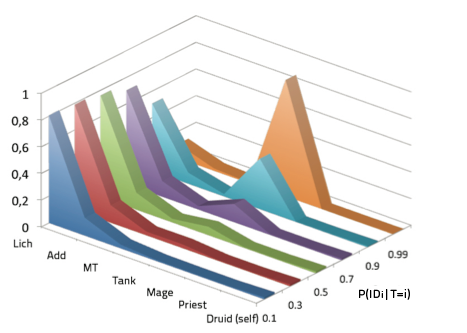
\includegraphics[width=7.8cm]{images/wow_distrib_target1.png} 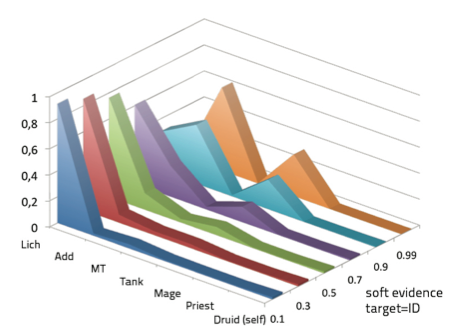
\includegraphics[width=7.8cm]{images/wow_distrib_target2.png}
\caption{Left: probabilities of targets depending on the soft evidence that a target is dying ($\PP(ID_i=true | T=i)$) with setup A (no ally is risking death). Right: same, with setup B (the ``tank'' ally is risking death).}
\label{fig:wow_target}
\end{center}
\end{figure}
\begin{figure}[h!]
\begin{center}
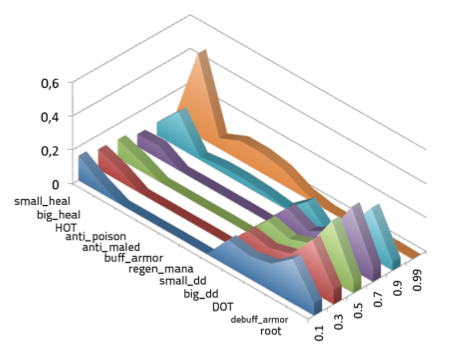
\includegraphics[width=7.8cm]{images/wow_distrib_skill1.png} 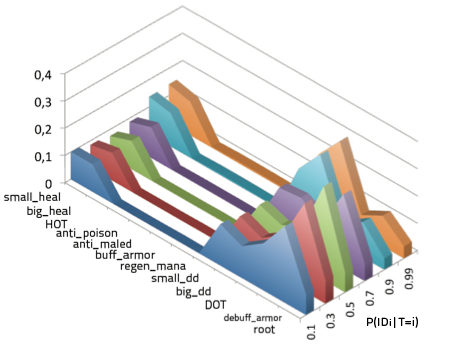
\includegraphics[width=7.8cm]{images/wow_distrib_skill2.png}
\caption{Left: Probabilities of skills depending on the soft evidence that a target is dying ($\PP(ID_i=true|T=i)$) with setup A (no ally is risking death). Right: same, with setup B (the ``tank'' ally is risking death).}
\label{fig:wow_skill}
\end{center}
\end{figure}

For the ``skill selection'' model, we can see on Fig.~\ref{fig:wow_skill} the influence of $ID_i$ on Skill which is coherent with the Target distribution: either, in setup A (left), we evolve with the increase of $\PP(ID_i=true|Target=i)$ to choose to heal our ally or, in setup B (right), to deal direct damage (and hopefully, kill) the foe attacking him. As you can see here, when we have the highest probability to attack the main enemy (``Lich'', when $\PP(ID_i=true|Target=i)$ is low), who is a $C=tank$, we get a high probability for the Skill \textit{debuff\_armor}. We only cast this skill if the debuff is not already present, so perhaps that we will cast \textit{small\_dd} instead. To conclude this example, Fig.~\ref{fig:wow_target_skill} shows the distribution on $\PP(T,S|all\_status\_variables)$ with setup A and the probability to target the previous target (set to ``Lich'' here) only $\approx 2$ times greater than any other character (so that we focus less on the same character), soft evidences $\PP(ID_i=true|Target=i)=0.9$ and $\PP(A_i=false|Target=i)=0.6$. On the decision-making side of this model, a simple approach would be a greedy one: if the first couple $(T,S)$ is already done or not available, we perform the second, and so on.


\begin{figure}[h!]
\begin{center}
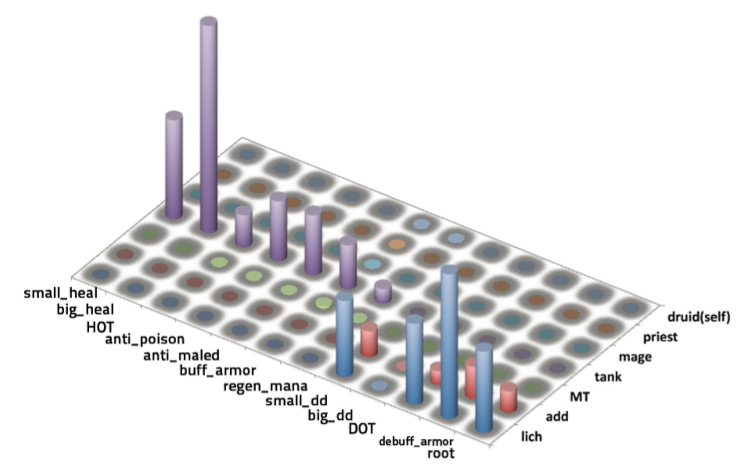
\includegraphics[width=12.5cm]{images/wow_distrib_target_skill.png}
\caption{Log-probabilities of Target and Skill with setup A, and $\PP(ID_i=true|T=i)=0.9, \PP(A_i=false|T=i)=0.6$. This plot corresponds to the answer to the full question on which decision-making has to be done.}
\label{fig:wow_target_skill}
\end{center}
\end{figure}

\subsection{Discussion}
%%% 
%%% This model has to be applied in a real MMORPG, out of its simulated sandbox, to reveal all its shortcomings and be updated. We can already think of some future difficulties, for instance there is a possibility for many games that the Skill variable will be very big and that it will imply a too high computational cost. For that concern, we propose to clusterize the skills in global skills ($GS$) (as it can be seen in the description of the example). This approach to break down the complexity of computation is general and can be used with other variables. The skill variable $S$ can then be the subset of skills corresponding to the clustering of $GS$, for instance we could have:
%%% 
%%% $$GS \in \{SkillHeal, SkillBuff, SkillAttack, SkillDebuff\}$$
%%% $$S = SkillHeal \in \{skill_1 \dots skill_j\}$$
%%% $$S = SkillBuff \in \{skill_{j+1} \dots skill_k\}$$
%%% $$S = SkillAttack \in \{skill_{k+1} \dots skill_l\}$$
%%% $$S = SkillDebuff \in \{skill_{l+1} \dots skill_m\}$$
%%% 
%%% Global skills joint distribution: as for the “Skill joint distribution” without Resists. It will take advantage of splitting between allies and foes.
%%% 
%%% \begin{eqnarray*}
%%% P(GS,T,HP_{1:n},D_{1:n},A_{1:n},\Delta HP_{1:n}, ID_{1:n}, C_{1:n}) = \\
%%% P(GS).P(T).\prod_{i=1}^n [ P(HP_i | A_i, C_i, GS, T).P(D_i | A_i, GS, T).P(A_i | GS, T)\\
%%%                         .P(\Delta HP_i | A_i, GS, T).P(ID_i | GS, T).P(C_i | A_i, GS, T)]
%%% \end{eqnarray*}
%%% 
%%% Specialized skills joint distribution:
%%% 
%%% \begin{eqnarray*}
%%% P(S,GS,T,HP_{1:n},D_{1:n},A_{1:n},\Delta HP_{1:n}, ID_{1:n}, C_{1:n}, R_{1:n}) = \\
%%% P(S|GS).P(T).\prod_{i=1}^n [ P(HP_i | A_i, C_i, S, T).P(D_i | A_i, S, T).P(A_i | S, T)\\
%%%                         .P(\Delta HP_i | A_i, S, T).P(R_i | C_i, S, T).P(ID_i | S, T).P(C_i | A_i, S, T)]
%%% \end{eqnarray*}
%%% for the corresponding S. So that we can ask the question:
%%% $$P(S | GS, T, hp_{1:n}, d_{1:n}, a_{1:n}, \Delta hp_{1:n}, id_{1:n}, c_{1:n}, r_{1:n})$$
%%% 
%%% that will trigger $P(GS|T,\dots)$, itself triggering $P(T|all\_state\_variables)$. Choosing to do with or without the intermediate $GS$ computation, regrouping abilities by types, is mainly a question of computational time.

This limited model served the purpose of presenting Bayesian programming in practice. While it was used in a simulation, it showcases the approach one can take to break down the problem of autonomous control of \glos{npc}. The choice of the skill or ability to use and the target on which to use it puts hard constraints on every others decisions the autonomous agent has to take to perform its ability action. Thus, such a model shows that:
\begin{itemize}
    \item cooperative behavior is not too hard to incorporate in a decision (instead of being hard-coded),
    \item it can be learned, either from observations of a human player or by reinforcement (exploration),
    \item it is computationally tractable (for use in all games), the inference is just a series of ``probabilistic \textit{if}s'',
\end{itemize}
Moreover, using this model on another agent than the one controlled by the AI can give a prediction on what it will do, resulting in human-like, adaptive, playing style.

We did not kept at the research track of Bayesian modeling MMORPG games due to the difficulty to work on these types of games: the studios have too much to lose to ``farmer'' bots to accept any automated access to the game. Also, there are no sharing format of data (like replays) and the invariants of the game situations are fewer than in RTS games. Finally, RTS games have international AI competitions which were a good motivation to compare our approach with other game AI researchers.

\chapter{RTS AI: \textit{StarCraft: Broodwar}}
\label{chapter:rtsai}
\newglossaryentry{micro}{name=micro-management,description={gameplay actions that are manually addressed by the player; the way of maximizing one's army efficiency by using the units to the maximum of their potential.}}

\begin{quotation}\textit{
We think of life as a journey with a destination (success, heaven). But we missed the point. It was a musical thing, we were supposed to sing and dance while music was being played.}\\
\begin{flushright}Alan Watts\end{flushright}
\end{quotation}

\lettrine{T}{his} chapter explains the basics of RTS gameplay, particularly StarCraft. We then list the (computational) challenges brought by RTS gameplay. We present a transversal decomposition of the RTS AI domain in levels of abstractions (strategy, tactics, \glos{micro}), which we will use for the rest of the dissertation.

\ifthenelse{\equal{\myebookformat}{false}}{
\chaptertoc
}{}

\section{How does the game work}

\subsection{RTS Gameplay}
\label{sec:rtsgameplay}
We first introduce the basic components of a real-time strategy (RTS) game. The player is usually referred as the ``commander'' and perceives the world in an allocentric ``God's view'', performing mouse and keyboard actions to give orders to units (or squads of units) within a circumvented area (the ``map''). In a RTS, players need to gather resources to build military units and defeat their opponents. To that end, they often have \textit{worker units} (or extraction structures) than can gather resources needed to build \textit{workers}, \textit{buildings}, \textit{military units} and \textit{research upgrades}. Workers are often also builders (as in StarCraft) and are weak in fights compared to military units. Resources may have different uses, for instance in StarCraft: minerals are used for everything, whereas gas is only required for advanced buildings or military units, and technology upgrades. Buildings and research upgrades define technology trees (directed acyclic graphs) and each state of a 
\newglossaryentry{techtree}{name={tech tree},description={abbreviation for ``technological tree'', state of the technology (buildings, researches, upgrades) which are unlocked/available to a given player.}}
%\newglossaryentry{techtree}{name={tech tree},description={abbr. for ``technological tree'', the state of buildings and technologies evolution (technologies which are unlocked) of a given player}}
\glos{techtree} (or \newglossaryentry{buildtree}{name={build tree},description={abbrev. for ``buildings tree'', state of the buildings (and thus production) unlocked by a player}}\glos{buildtree}) allow for different unit type production abilities and unit spells/abilities. The military units can be of different types, any combinations of ranged, casters, contact attack, zone attacks, big, small, slow, fast, invisible, flying... In the end, a central part of the gameplay is that units can have attacks and defenses that counter each others as in a soft rock-paper-scissors. Also, from a player point of view, most RTS games are only partially observable due to the \textit{\glos{fogofwar}} which hides units and new buildings which are not in sight range of the player's units. 


In chronological order, RTS include (but are not limited to): Ancient Art of War, Herzog Zwei, Dune II, Warcraft, Command \& Conquer, Warcraft II, C\&C: Red Alert, Total Annihilation, Age of Empires, StarCraft, Age of Empires II, Tzar, Cossacks, Homeworld, Battle Realms, Ground Control, Spring Engine games, Warcraft III, Total War, Warhammer 40k, Sins of a Solar Empire, Supreme Commander, StarCraft II. The differences in gameplay are in the order of number, nature and gathering methods of resources; along with construction, research and production mechanics. The duration of games vary from 15 minutes for the fastest to (1-3) hours for the ones with the biggest maps and longest gameplays. We will now focus on StarCraft, on which our robotic player is implemented.


\subsection{A StarCraft Game}
\textit{StarCraft} is a science-fiction RTS game released by Blizzard Entertainment$^{TM}$ in March 1998. It was quickly expanded into \textit{StarCraft: Brood War} (SC: BW) in November 1998. In the following, when referring to StarCraft, we mean StarCraft with the Brood War expansion. StarCraft is a canonical RTS game in the sense that it helped define the genre and most gameplay mechanics seen in other RTS games are present in StarCraft. It is as much based on strategy than tactics, by opposition to the Age of Empires and Total Annihilation series in which strategy is prevalent. In the following of the thesis, we will focus on duel mode, also known as 1 vs. 1 (1v1). Team-play (2v2 and higher) and ``free for all'' are very interesting but were not studied in the framework of this research. These game modes particularly add a layer of coordination and bluff respectively.


StarCraft sold 9.5 millions licenses worldwide, 4.5 millions in South Korea alone \citep{StarCraftNumbers}, and reigned on competitive RTS tournaments for more than a decade. Numerous international competitions (World Cyber Games, Electronic Sports World Cup, BlizzCon, OnGameNet StarLeague, MBCGame StarLeague) and professional gaming (mainly in South Korea \citep{Chee05}) produced a massive amount of data of highly skilled human players. In South Korea, there are two TV channels dedicated to broadcasting competitive video games, particularly StarCraft. The average salary of a \glos{pro-gamer} there was up to 4 times the average South Korean salary \citep{MYMPGM} (up to \$200,000/year on contract for NaDa). Professional gamers perform about 300 actions (mouse and keyboard clicks) per minute while following and adapting their strategies, while their hearts reach 160 beats per minute (BPM are displayed live in some tournaments). StarCraft II is currently (2012) taking over StarCraft in competitive gaming but a) there is still a strong pool of highly skilled StarCraft players and b) StarCraft II has a really similar gameplay.


StarCraft (like most RTS) has a \textit{\glos{replay}} mechanism, which enables to record every player's actions such that the state of the game can be deterministically re-simulated. The only piece of stochasticity comes from ``attack miss rates'' ($\approx 47\%$) when a unit is on a lower ground than its target. These randomness generator seed is saved along with the actions in the replay. All high level players use this feature heavily either to improve their play or study opponents' styles. Observing replays allows player to see what happened under the \textit{\glos{fogofwar}}, so that they can understand timing of technologies and attacks, and find clues/evidences leading to infer the strategy as well as weak points.


In StarCraft, there are three factions with very different units and technology trees:
\begin{itemize}
    \item \textit{Terran}: humans with strong defensive capabilities and balanced, averagely priced biological and mechanical units.
    \item \textit{Protoss}: advanced psionic aliens with expensive, slow to produce but resistant units.
    \item \textit{Zerg}: insectoid alien race with cheap, quick to produce but weak units.
\end{itemize}

All factions use workers to gather resources, and all other characteristics are different: from military units to ``\gloss{techtree}'', gameplay styles. Races are so different that highly skilled players focus on playing with a single race (but against all three others). There are two types of resources, often located close together, minerals and gas. From minerals, one can build basic buildings and units, which opens the path to more advanced buildings, technologies and units, which will in turn all require gas to be produced. While minerals can be gathered at an increasing rate (bounded asymptotically) the more workers are put at work, the gas gathering rate is quickly limited to 3 workers per gas geyser (i.e. per base). There is another third type of ``special'' resource, called \newglossaryentry{supply}{name=supply,description={cost in population (or supply) of a given unit, or current population count of a player.}}\textit{\glos{supply}}, which is the current population of a given player (or the cost in population of a given unit), and \newglossaryentry{maxsupply}{name={max supply},description={maximum number of units that a player can control at a given time, can be increased up to a hard limit (200 in StarCraft).}}\textit{\glos{maxsupply}}, which is the current limit of population a player can control. \Glos{maxsupply} can be upgraded by building special buildings (Protoss Pylon, Terran Supply Depot) or units (Zerg Overlord), giving 9 to 10 additional \glos{maxsupply}, up to a hard limit of 200. Some units cost more supply than others (from 0.5 for a Zergling to 8 for a Protoss Carrier or Terran Battlecruiser). In Figure~\ref{fig:SC_eco}, we show the very basics of Protoss economy and buildings. Supply will sometimes be written supply/max supply (supply on max supply). For instance 4/9 is that we currently have a population of 4 (either 4 units of 1, or 2 of 2 or ...) on a current maximum of 9. %In Figure~\ref{fig:SC_battle}, we show

\newglossaryentry{mini-map}{name=mini-map,description={radar view of the full game area, shown in the bottom corner of the interface in StarCraft.}}
\begin{figure}[!ht]
\begin{center}
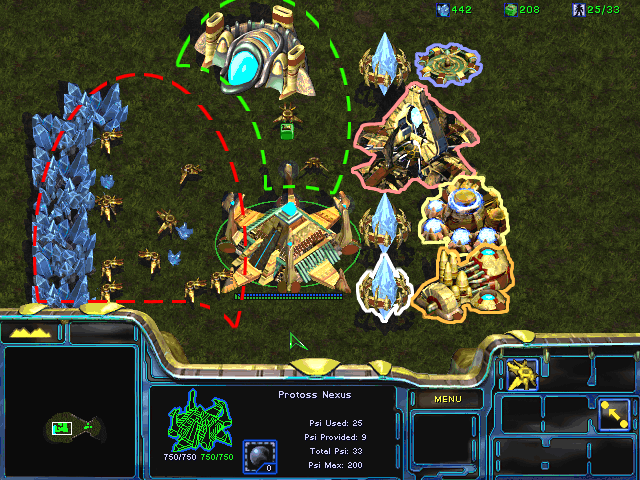
\includegraphics[width=14cm]{images/SC_eco.png}
\caption{A StarCraft screenshot of a Protoss base, with annotations. The interface (heads up display at the bottom) shows the \textit{\glos{mini-map}}. The center of the interface (bottom) shows the selected unit (or group of units), here the Protoss Nexus (main economical building, producing workers and to which resources are brought) which is in the center of the screen and circled in green. The bottom right part shows the possible actions (here build a Protoss Probe or set a rally point). The top right of the screen shows the minerals (442), gas (208) and \glos{supply} (25 total) on \glos{maxsupply} (33). The dotted lines demarcate economical parts with active workers: red for minerals mining and green for gas gathering. The plain cut outs of buildings show: a Pylon (white), a Forge (orange, for upgrades and access to static defense), a Cybernetics Core (yellow, for technological upgrades and expanding the tech tree), a Gateway (pink, producing ground units), a Photon Cannon (blue, static defense).}
\label{fig:SC_eco}
\end{center}
\end{figure}

\newglossaryentry{opening}{name=opening,description={in Chess as in RTS games: the first strategic moves of the game, the strategy of the early game},plural=openings}
\newglossaryentry{buildorder}{name=build order,description={a formal specification of timings (most often indexed on total population count) at which to perform build actions in the early game.}}
To reach a competitive amateur level, players have to study \textit{\gloss{opening}} and hone their \textit{\gloss{buildorder}}. An opening corresponds to the first strategic moves of a game, as in other abstract strategy games (Chess, Go). They are classified/labeled with names from high level players. A build-order is a formally described and accurately timed sequence of buildings to construct in the beginning. As there is a bijection between optimal population and time (in the beginning, before any fight), build orders are indexed on the total population of the player as in the example for Protoss in table~\ref{bo:two_gates_goon_range}. 
At the highest levels of play, StarCraft games usually last between 6 (shortest games, with a successful rush from one of the player) to 30 minutes (long economically and technologically developed game).
%%%\begin{verbatim}
%%%population-thing to build
%%%8-Pylon 
%%%10-Gateway 
%%%12-Gas Assimilator
%%%13-Make Zealot Once Gateway completes 
%%%16-Pylon 
%%%18-Core
%%%20-Make Zealot 
%%%22-Pylon, make Dragoon
%%%27-Start Dragoon Range Upgrade, Pylon 
%%%30-Robotics Facility, Gateway
%%%32-Pylon 
%%%37-Make Shuttle, Start cutting Probes (don't make probes anymore for now) 
%%%39-Observatory, Then Robotic Support Bay
%%%43-make observer 
%%%44-Pylon 
%%%48-Make Reaver 
%%%52-Pylon, Start Back Probe Production (make probes again) 
%%%\end{verbatim}
\begin{table}[ht]
\begin{center}
\begin{tabular}{|l|l|l|}
\hline
Supply/Max supply & Build & Note \\
(population/max) & or Product & \\
\hline
8/9 & Pylon & ``supply/psi/control/population'' building \\
10/17 & Gateway & units producing structure \\
12/17 & Assimilator & constructed on a gas geyser, to gather gas \\
14/17 & Cybernetics Core & technological building \\
16/17 & Pylon & ``supply/psi/control/population'' building \\
16/17 & Range & it is a research/tech \\
17/25 & Dragoon & first military unit \\
\hline
\end{tabular}
\end{center}
\caption{An example of the beginning of a ``2 Gates Goon Range'' Protoss build order which focus on building dragoons and their attack range upgrade quickly.}
\label{bo:two_gates_goon_range}
\end{table}

%``Cutting'' workers (here, Probes for Protoss) production is a common feat of highly optimized ``timing attacks'' builds.
\begin{figure}[!ht]
\begin{center}
\begin{tabular}{cc}
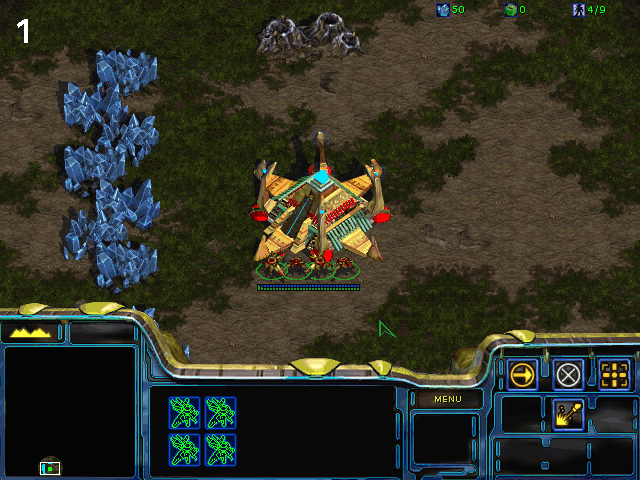
\includegraphics[width=8cm]{images/SC_game/SC_start_game.png} &
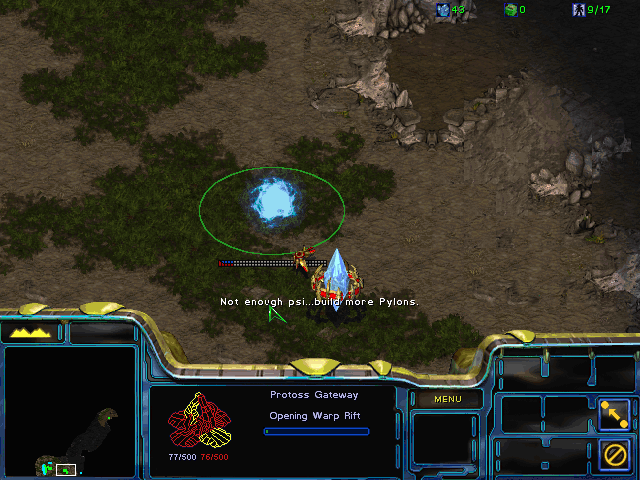
\includegraphics[width=8cm]{images/SC_game/SC_first_gate.png} \\
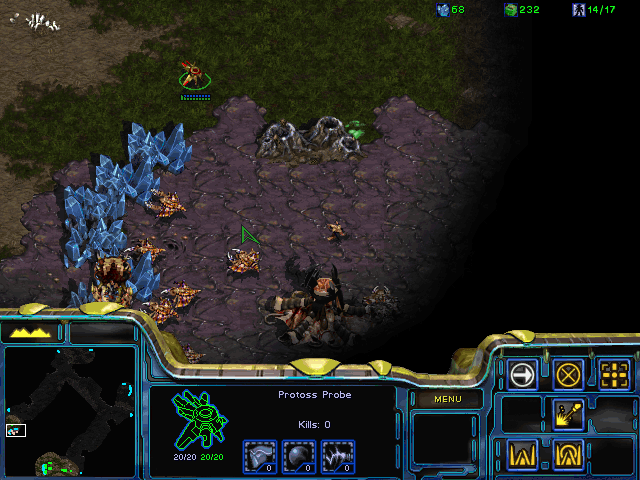
\includegraphics[width=8cm]{images/SC_game/SC_scout_opponent.png} & 
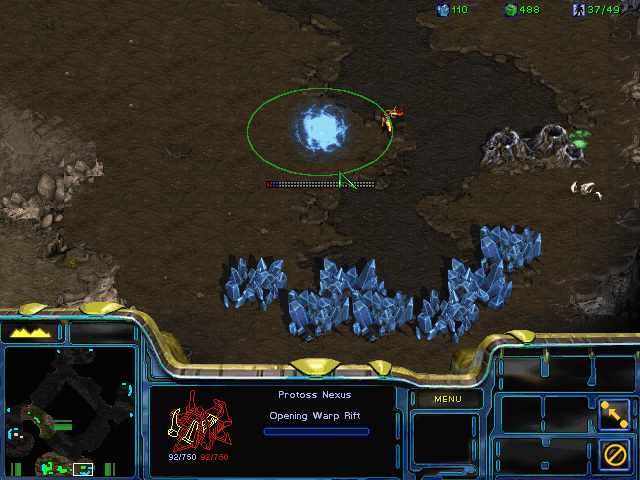
\includegraphics[width=8cm]{images/SC_game/SC_expand.png} \\ 
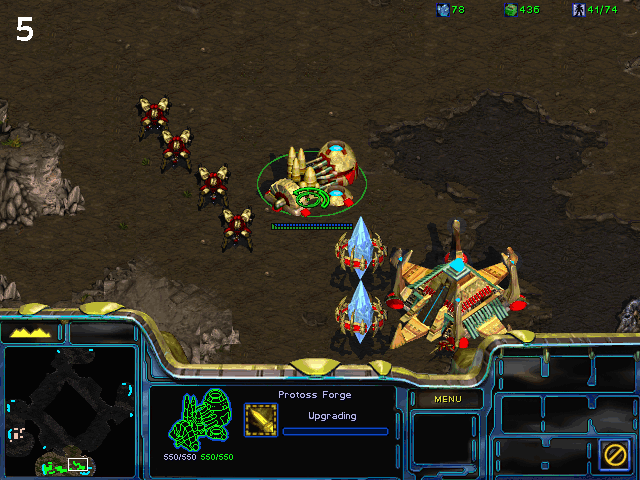
\includegraphics[width=8cm]{images/SC_game/SC_upgrade_attack.png} & 
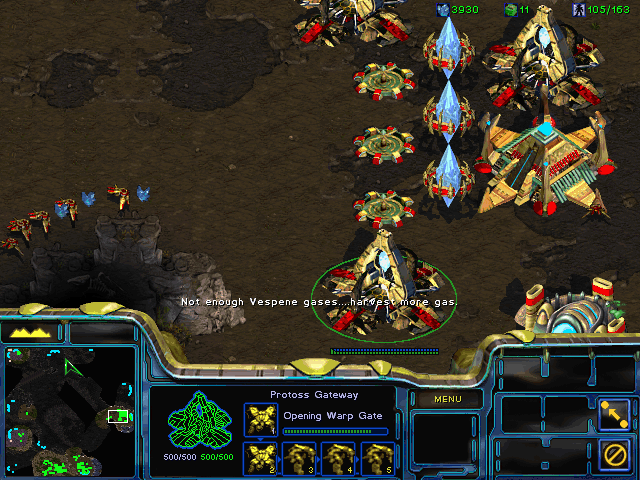
\includegraphics[width=8cm]{images/SC_game/SC_queue_production.png}
\end{tabular}
%SC_first_pylon.png
\caption{Start and economical parts of a StarCraft game. The order of the screenshots goes from left to right and from top to bottom.}
\label{fig:SC_game1}
\end{center}
\end{figure}

\begin{figure}[!ht]
\begin{center}
\begin{tabular}{cc}
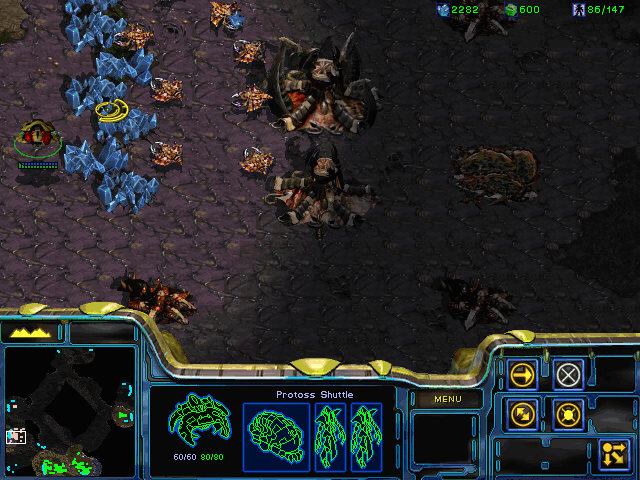
\includegraphics[width=8cm]{images/SC_game/SC_drop2a.png} &
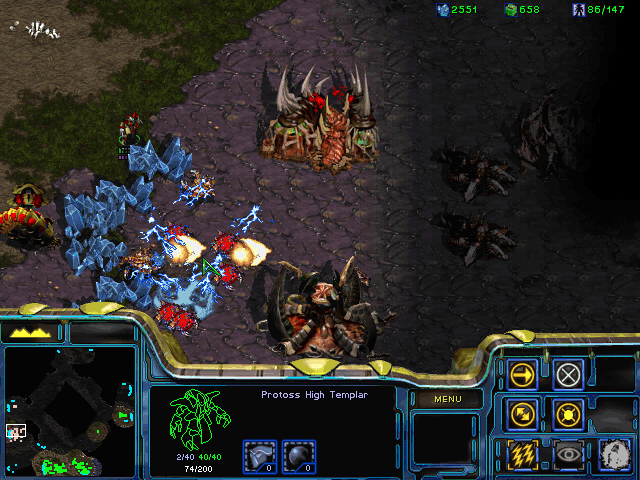
\includegraphics[width=8cm]{images/SC_game/SC_drop2b.png} \\
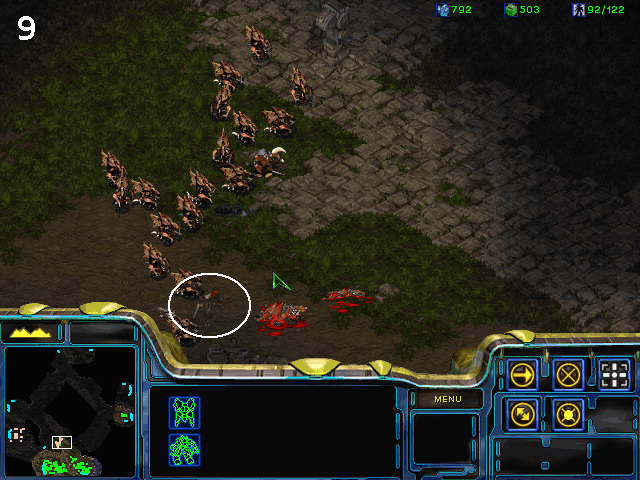
\includegraphics[width=8cm]{images/SC_game/SC_dt_army.png} & 
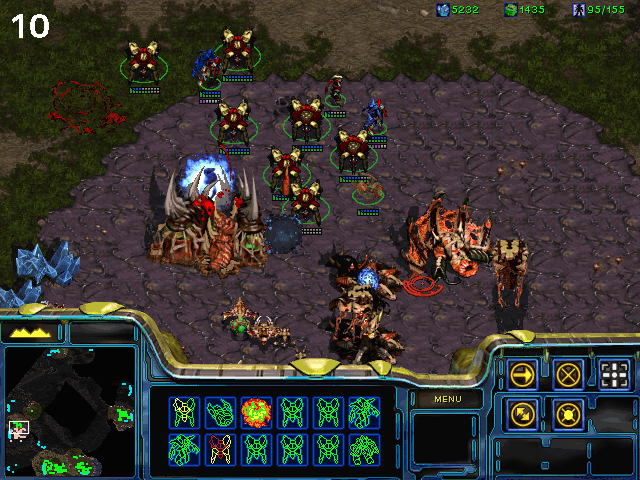
\includegraphics[width=8cm]{images/SC_game/SC_final_attack.png}
\end{tabular}
\caption{Military moves from a StarCraft (PvT) game. The order of the screenshots goes from left to right and from top to bottom.}
\label{fig:SC_game2}
\end{center}
\end{figure}

We now present the evolution of a game (Figures~\ref{fig:SC_game1} and \ref{fig:SC_game2}) during which we tried to follow the build order presented in table~\ref{bo:two_gates_goon_range} (``2 Gates Goon Range''\footnote{On Teamliquid: \url{http://wiki.teamliquid.net/starcraft/2_Gate_Goon_Range_(vs._Terran)}}) but we had to adapt to the fact that the opponent was Zerg (possibility for a faster rush) by building a Gateway at 9 supply and building a Zealot (ground contact unit) before the first Dragoon. The first screenshot (image 1 in Figure~\ref{fig:SC_game1}) is at the very start of the game: 4 Probes (Protoss workers), and one Nexus (Protoss main building, producing workers and depot point for resources). At this point players have to think about what \gloss{opening} they will use. Should we be aggressive early on or opt for a more defensive opening? Should we specialize our army for focused tactics, to the detriment of being able to handle situations (tactics and armies compositions) from the opponent that we did not foresee? In picture 2 in the same Figure (\ref{fig:SC_game1}), the first gate is being built. At this moment, players often send a worker to ``scout'' the enemy's base, as they cannot have military units yet, it is a safe way to discover where they are and inquiry about what they are doing. In picture 3, the player scouts their opponent, thus gathering the first bits of information about %their race (which is known beforehand if not playing against ``Random'') and 
their early tech tree. Thus, knowing to be safe from an early attack (``rush''), the player decides to go for a defensive and economical strategy for now. Picture 4 shows the player ``expanding'', which is the act of making another base at a new resource location, for economical purposes. In picture 5, we can see the upgrading of the ground weapons along with 4 ranged military units, staying in defense at the expansion. This is a technological decision of losing a little of potential ``quick military power'' (from military units which could have been produced for this minerals and gas) in exchange of global upgrade for all units (alive and to be produced), for the whole game. This is an investment in both resources and time. Picture 6 showcases the production queue of a Gateway as well as workers transferring to a second expansion (third base). Being safe and having expanded his \glos{techtree} to a point where the army composition is well-rounded, the player opted for a strategy to win by profiting from an economical lead. Figure~\ref{fig:SC_game2} shows the aggressive moves of the same player: in picture 7, we can see a flying transport with artillery and area of effect ``casters'' in it. The goal of such an attack is not to win the game right away but to weaken the enemy's economy: each lost worker has to be produced, and, mainly, the missing gathering time adds up quite quickly. In picture 8, the transport in unloaded directly inside the enemy's base, causing huge damages to their economy (killing workers, Zerg Drones). This is the use of a specialized tactics, which can change the course of a game. At the same time, it involves only few units (a flying transport and its cargo), allowing for the main army to stay in defense at base. It capitalizes on the maneuverability of the flying Protoss Shuttle, the technological advancements allowing area of effects attacks and the large zone that the opponent has to cover to defend against it. In picture 9, an invisible attacking unit (circled in white) is harassing the oblivious enemy's army. This is an example of how technology advance on the opponent can be game changing (the opponent does not have detection in range, thus is vulnerable to cloaked units). Finally, picture 10 shows the final attack, with a full ground army marching on the enemy's base.


\section{RTS AI Challenges}
\label{sec:rtsaichallenges}
In combinatorial game theory terms, competitive StarCraft (1 versus 1) is a zero sum, partial-information, deterministic\footnote{The only stochasticity is in attacks failures (miss rate) from lower grounds to higher grounds, which is easily averaged.} strategy game. 
StarCraft subsumes Wargus (Warcraft II open source clone), which has an estimated mean branching factor $1.5.10^3$ \citep{LTW} (Chess: $\approx 35$, Go: $<360$): \cite{bgweberPhD} finds a branching factor greater than $1.10^6$ for StarCraft. In a given game (with maximum map size) the number of possible positions is roughly of $10^{11500}$, versus the Shannon number for Chess ($10^{43}$) \citep{Shannon_1950}. Also, we believe strategies are much more balanced in StarCraft than in most other games. Otherwise, how could it be that more than a decade of professional gaming on StarCraft did not converge to a finite set of fixed (imbalanced) strategies?

Humans deal with this complexity by abstracting away strategy from low level actions: there are some highly restrictive constraints on where it is efficient (``optimal'') to place economical main buildings (Protoss Nexus, Terran Command Center, Zerg Hatchery/Lair/Hive) close to minerals spots and gas geysers. Low-level \glos{micro} decisions have high \textit{horizontal continuity} and humans see these tasks more like playing a musical instrument skillfully. Finally, the continuum of strategies is analyzed by players and some distinct strategies are identified as some kinds of ``invariants'', or ``entry points'' or ``principal components''. From there, strategic decisions impose some (sometimes hard) constraints on the possible tactics, and the complexity is broken by considering only the interesting state space due to this high \textit{vertical continuity}.

Most challenges of RTS games have been identified by \citep{Buro03,Buro04callfor}. We will try to anchor them in the human reasoning that goes on while playing a StarCraft game.
\begin{itemize}
    \item \textit{Adversarial planning under uncertainty} (along with \textit{resource management}): it diverges from traditional planning under uncertainty in the fact that the player also has to plan \textit{against} the opponent's strategy, tactics, and actions. From the human point of view, he has to plan for which buildings to build to follow a chosen \glos{opening} and subsequent strategies, under a restricted resources (and time) budget. At a lower level, and less obvious for humans, are the plans they make to coordinate units movements.
    \item \textit{Learning and opponent modeling}, Buro accurately points out that human players need very few (``a couple of'') games to spot their opponents' weaknesses. Somehow, human opponent modeling is related to the ``induction scandal'', as Russell called it: how do humans learn so much so fast? We learn from our mistakes, we learn the ``play style'' of our opponent's, we are quickly able to ask ourselves: ``what should I do now given what I have seen \textit{and} the fact that I am playing against player XYZ?''. ``Could they make the same attack as last time?''. To this end, we use high level representations of the states and the actions with compressed invariants, causes and effects.
    \item \textit{Spatial and temporal reasoning} (along with \textit{decision making under uncertainty}), this is related to planning under uncertainty but focuses on the special relations between what can and what cannot be done in a given time. Sadly, it was true in 2004 but is still true today: ``RTS game AI [...] falls victim to simple common-sense reasoning''. Humans learn sequences of actions, and reason only about actions coherent with common sense. For AI of complex systems, this common-sense is hard to encode and to use.
    %\item Resource management
    %\item Decision making under uncertainty
    \item Collaboration (teamplay), which we will not deal with here: a lot has to do with efficient communication and ``teammate modeling''.
\end{itemize}
As we have seen previously more generally for multi-player video games, all these challenges can be handled by Bayesian modeling. %The Cox-Jaynes theorem particularly comes to mind from ``induction scandal'' 
While acknowledging these challenges for RTS AI, we now propose a different task decomposition, in which different tasks will solve some parts of these problems at their respective levels.

% TODO ?


\section{Tasks decomposition and linking}
\begin{figure}[!ht]
\begin{center}
\begin{small}
\ifthenelse{\equal{\myebookformat}{true}}{
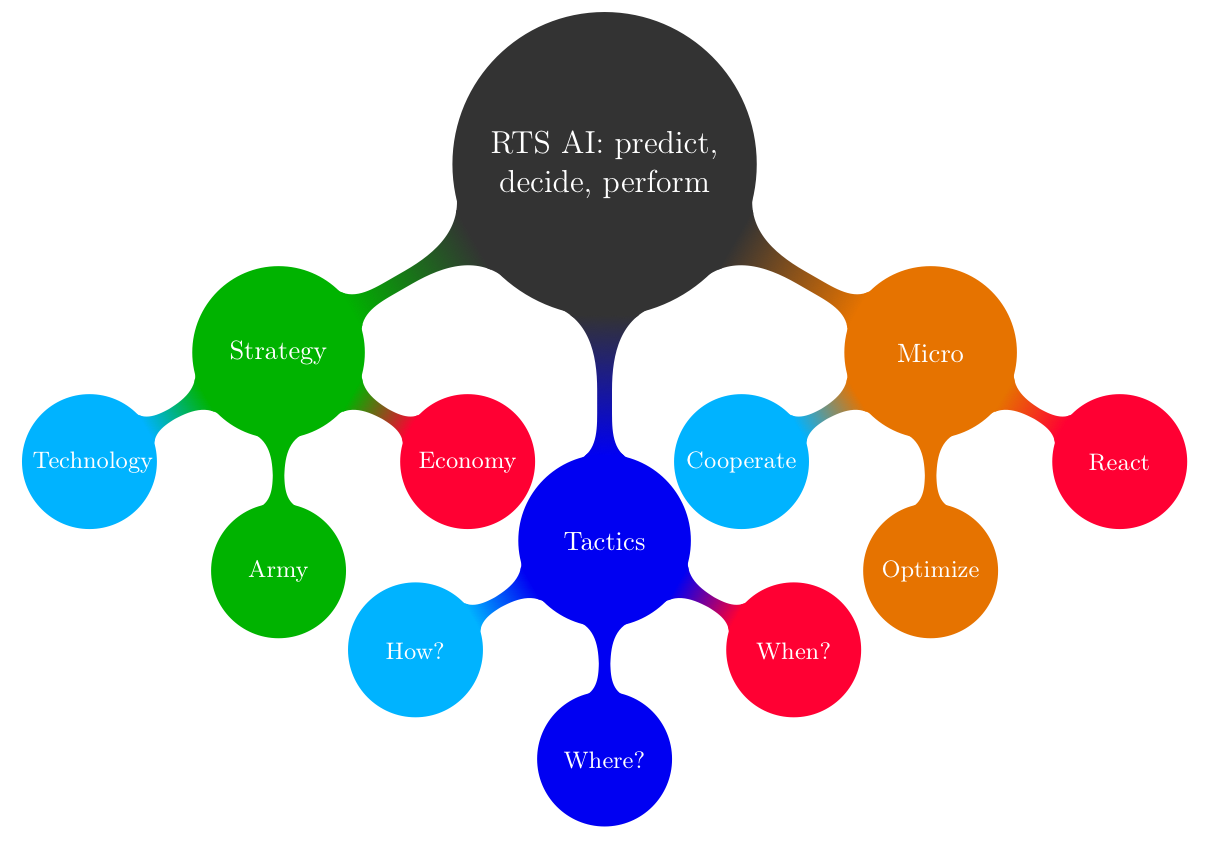
\includegraphics[width=12cm]{images/tikz7.png}
}{
\begin{tikzpicture}
  \path[mindmap,concept color=black!80!white,text=white]
    node[concept] {RTS AI: predict, decide, perform}
    [clockwise from=-30]
    child[concept color=orange!90!black] {
      node[concept] {Micro}
      child[concept color=red!80!magenta] { node[concept] {React} }
      child { node[concept] {Optimize} }
      child[concept color=blue!30!cyan] { node[concept] {Cooperate} }
    }
    child[concept color=blue!95!black] { % TODO change color
      node[concept] {Tactics}
      child[concept color=red!80!magenta] { node[concept] {When?} }
      child { node[concept] {Where?} }
      child[concept color=blue!30!cyan] { node[concept] {How?} }
    }
    child[concept color=green!70!black] {
      node[concept] {Strategy}
      child[concept color=red!80!magenta] { node[concept] {Economy}} %{Initiative} }
      child { node[concept] {Army}} %{Army composition} }
      child[concept color=blue!30!cyan] { node[concept] {Technology}} %{Spendings balance} }
    };  
\end{tikzpicture}
}
\end{small}
\end{center}
\caption{A mind-map of RTS AI. This is the tasks decomposition that we will use for the rest of the thesis.}
\label{fig:mindmapRTS}
\end{figure}

We decided to decompose RTS AI in the three levels which are used by the gamers to describe the games: \textit{strategy}, \textit{tactics}, \textit{micro-management}. We remind the reader that parts of the map not in the sight range of the player's units are under \textit{\glos{fogofwar}}, so the player has only partial information about the enemy buildings and army. The way by which we expand the tech tree, the specific units composing the army, and the general stance (aggressive or defensive) form what we call \textit{strategy}. At the lower level, the actions performed by the player (human or not) to optimize the effectiveness of its units is called \textit{\glos{micro}}. In between lies \textit{tactics}: where to attack, and how. A good human player takes much data in consideration when choosing: are there flaws in the defense? Which spot is more worthy to attack? How much am I vulnerable for attacking here? Is the terrain (height, chokes) to my advantage? The concept of strategy is a little more abstract: at the beginning of the game, it is closely tied to the build order and the intention of the first few moves and is called the \textit{opening}, as in Chess. Then, the long term strategy can be partially summed up by three signals/indicators:
\begin{itemize}
    \item aggression: how much is the player aggressive or defensive?
    \item initiative: how much is the player adapting to the opponent's strategy vs. how much is the player being original?
    \item technology/production/economy (tech/army/eco) distribution of resources: how much is the player spending (relatively) in these three domains?
\end{itemize}
\newglossaryentry{expand}{name=expand,description={either placement of a new base or the action to take a new base (to collect more resources).}}
At high levels of play, the tech/army/eco balance is putting a hard constraint on the aggression and initiative directions: if a player invested heavily in their army production, they should attack soon to leverage this investment. To the contrary, all other things being equal, when a player \gloss{expand}, they are being weak until the expansion repaid itself, so they should play defensively. Finally, there are some technologies (researches or upgrades) which unlocks an ``attack timing'' or ``attack window'', for instance when a player unlocks an invisible technology (or unit) before that the opponent has detection technology (detectors). On the other hand, while ``teching'' (researching technologies or expanding the \glos{techtree}), particularly when there are many intermediate technological steps, the player is vulnerable because of the immediate investment they made, which did not pay off yet.

From this RTS domain tasks decomposition, we can draw the mind map given in Figure~\ref{fig:mindmapRTS}. We also characterized these levels of abstractions by:
\begin{itemize}
    \item the conditioning that the decisions on one abstraction level have on the other, as discussed above: strategy conditions tactics which conditions low-level actions (that does not mean than there cannot be some feedback going up the hierarchy).
    \item the quantity of direct information that a player can hope to get on the choices of their opponent. While a player can see directly the micro-management of their enemy (movements of units on the battlefront), they cannot observe all the tactics, and a big part of tactics gameplay is to hide or fake them well. Moreover, key technological buildings are sometimes hidden, and the player has to form beliefs about the long term strategy of the opponent (without being in their head).
    \item the time which is required to switch behaviors of a given level. For instance a change of strategy will require to either \textit{a)} (technology) build at least two buildings or a building and a research/upgrade, \textit{b)} (army) build a few units, \textit{c)} take a new expansion (new base). A change of tactics corresponds to a large repositioning of the army(ies), while a change in micro-management is very quick (like moving units out of an area-of-effect damage zone).
\end{itemize}
This is shown in Figure~\ref{fig:sc_abstraction_times}. We will discuss the state of the art for the each of these subproblems (and the challenges listed above) in their respective parts.

\begin{figure}[htp]
\centerline{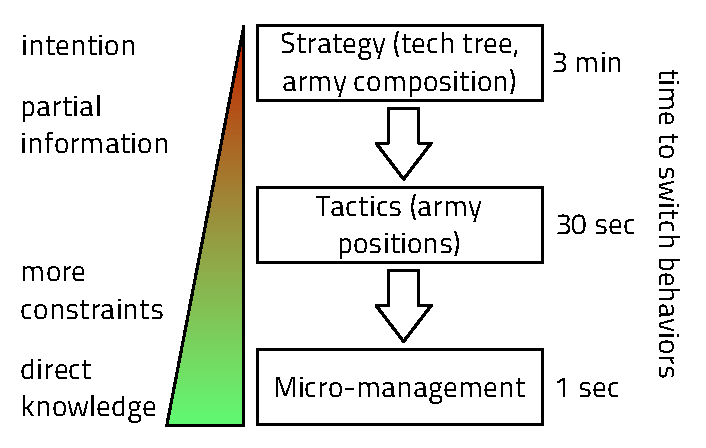
\includegraphics[width=7cm]{images/starcraft_levels_abstraction_light.pdf}}
\caption{Gameplay levels of abstraction for RTS games, compared with their level of direct (and complete) information and orders of magnitudes of time to chance their policies.}
\label{fig:sc_abstraction_times}
\end{figure}


To conclude, we will now present our works on these domains in separate chapters:
\begin{itemize}
    \item Micro-management: chapter~\ref{chapter:micro},
    \item Tactics: chapter~\ref{chapter:tactics},
    \item Strategy: chapter~\ref{chapter:strategy},
    \item Robotic player (bot): chapter~\ref{chapter:bot}.
\end{itemize}
In Figure~\ref{fig:conceptbbq}, we present the flow of informations between the different inference and decision-making parts of the bot architecture. One can also view this problem as having a good model of one's strategy, one's opponent strategy, and taking decisions. The software architecture that we propose is to have services building and maintaining the model of the enemy as well as our state, and decision-making modules using all this information to give orders to actuators (filled in gray in Fig.~\ref{fig:conceptbbq}).

\begin{figure}[!ht]
\begin{center}
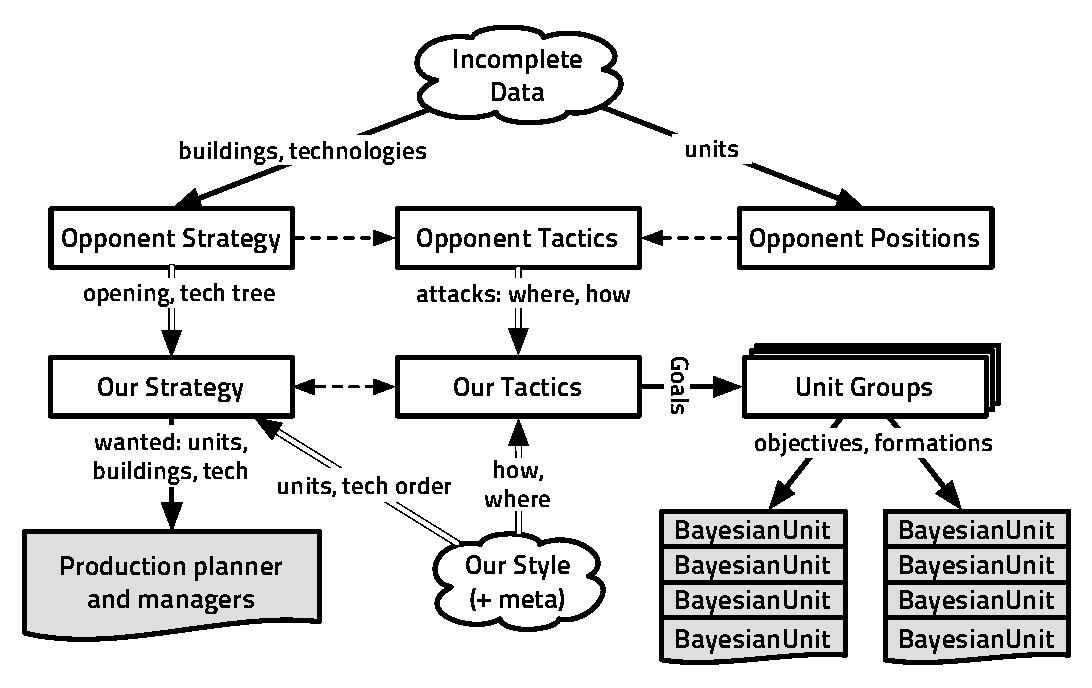
\includegraphics[width=16cm]{images/starcraft_bbq_concept.pdf}
\end{center}
\caption{Information-centric view of the architecture of the major components of the bot. Arrows are labeled with the information or orders they convey: dotted arrows are conveying constraints, double lined arrows convey distributions, plain and simple arrows convey direct information or orders. The gray parts perform game actions (as the physical actions of the player on the keyboard and mouse).}
\label{fig:conceptbbq}
\end{figure}



\chapter{Micro-management}
\label{chapter:micro}
\begin{quotation}
\noindent
\textit{La vie est la somme de tous vos choix.
\vspace{0.2cm}\\
Life is the sum of all your choices.}
%\vspace{0.2cm}\\
\begin{flushright}Albert Camus\end{flushright}
\end{quotation}

\lettrine{W}{e} present a Bayesian sensory-motor model for multi-agent (decentralized) units control in an adversarial setting. Orders, coming from higher up in the decision hierarchy, are integrated as another sensory input. We evaluated our model on classic StarCraft \glos{micro} tasks. This work was published at Computational Intelligence in Games (IEEE CIG) 2011 in Seoul \citep{SYNNAEVE:Micro}.

\ifthenelse{\equal{\myebookformat}{false}}{
\chaptertoc
}{}
\newacronym{RL}{RL}{reinforcement learning}

\begin{itemize}
\item \underline{Problem:} optimal control of units in a (real-time) huge adversarial actions space (collisions, accelerations, terrain, damages, areas of effects, foes, goals...).
\item \underline{Problem that we solve:} efficient coordinated control of units incorporating all low level actions and inputs, plus higher level orders and representations.
\item \underline{Type:} it is a problem of \textit{multi-agent control in an adversarial environment}\footnote{Strictly, it can be modeled as a \glos{pomdp} for each unit independently with $S$ the states of all the other units (enemies and allied altogether) which are known through observations $O$ by conditional observations probabilities $\Omega$, with $A$ the set of actions for the given unit, $T$ transition probabilities between states and depending on actions, and the reward function $R$ based on goal execution, unit survivability and so on... It can also be viewed as a (gigantic) \glos{pomdp} solving the problem for all (controlled units) at once, the advantage is that all states $S$ for allied units is known, the disadvantage is that the combinatorics of $T$ and $A$ make it intractable for useful problems.}.
\item \underline{Complexity:} \textsc{pspace}-complete \citep{Papadimitriou87,GamingComplexity}. Our solutions are real-time on a laptop.
\end{itemize}

% TODO: 
% add graphical model??\\

\begin{figure}[ht]
\begin{center}
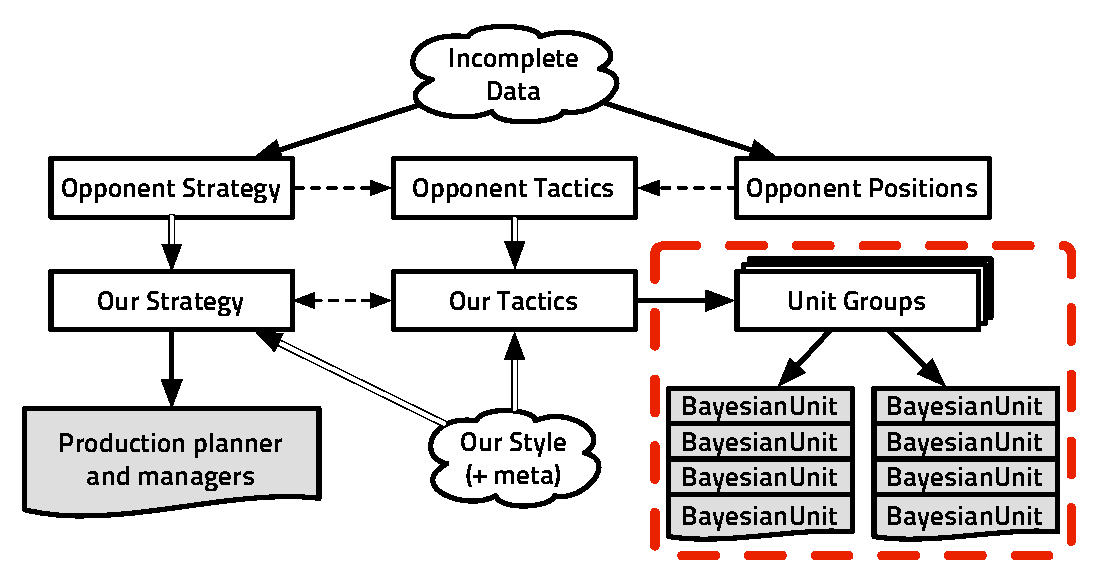
\includegraphics[width=0.84\columnwidth]{images/starcraft_bbq_concept_MICRO.pdf}
\end{center}
\caption{Information-centric view of the architecture of the bot, the part concerning this chapter (\glos{micro}) is in the dotted rectangle}
\label{fig:conceptMICRO}
\end{figure}

\section{Units Management}
\subsection{Micro-management complexity}
In this part, we focus on \glos{micro}, which is the lower-level in our hierarchy of decision-making levels (see Fig.~\ref{fig:sc_abstraction_times}) and directly affect units control/inputs. Micro-management consists in maximizing the effectiveness of the units \textit{i.e.} the damages given/damages received ratio. These has to be performed simultaneously for units of different types, in complex battles, and possibly on heterogeneous terrain. 
For instance: retreat and save a wounded unit so that the enemy units would have to chase it either boosts your firepower (if you save the unit) or weakens the opponent's (if they chase). 

StarCraft micro-management involves ground, flying, ranged, contact, static, moving (at different speeds), small and big units (see Figure~\ref{fig:sc_fight}). Units may also have splash damage, spells, and different types of damages whose amount will depend on the target size. It yields a rich states space and needs control to be very fast: human progamers can perform up to 400 ``actions per minute'' in intense fights. The problem for them is to know which actions are effective and the most rewarding to spend their actions efficiently. A robot does not have such physical limitations, but yet, badly chosen actions have negative influence on the issue of fights. %The problem is to identify what has to be done and what can be done, in real-time.

Let $\mathbf{U}$ be the set of the $m$ units to control, $\mathbf{A} = \{\cup_i\ \vec{d_i}\} \cup \mathbf{S}$ be the set of possible actions (all $n$ possible $\vec{d}$ directions, standing ground included, and $\mathbf{S}$kills, firing included), and $\mathbf{E}$ the set of enemies. As $|\mathbf{U}| = m$, we have $|\mathbf{A}|^{m}$ possible combinations each turn, and the enemy has $|\mathbf{A}|^{|\mathbf{E}|}$. 
The dimension of the set of possible actions each micro-turn (for instance: 1/24th of a second in StarCraft) constrains reasoning about the state of the game to be hierarchical, with different levels of granularity. In most RTS games, a unit can go (at least) in its 24 surrounding tiles (see Figure~\ref{fig:sc_fight}, each arrow correspond to a $\vec{d_i}$)
) %, combination of N, S, E, W up to the 2nd order), 
stay where it is, attack, and sometimes cast different spells: which yields more than 26 possible actions each turn. Even if we consider only 8 possible directions, stay, and attack, with $N$ units, there are $10^N$ possible combinations each turn (all units make a move each turn). As large battles in StarCraft account for \textit{at least} 20 units on each side, optimal units control hides in too big a search space to be fully explored in real-time (sub-second reaction at least) on normal hardware, even if we take only one decision per unit per second.

\begin{figure}
\begin{center}
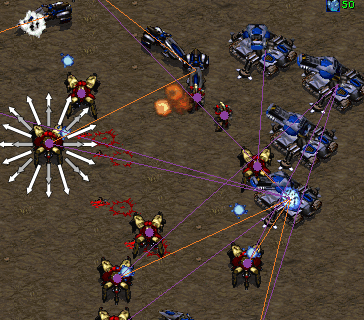
\includegraphics[width=8.6cm]{images/SC_fight_3b.png}
\end{center}
\caption{Screen capture of a fight in which our bot controls the bottom-left units in StarCraft. The 25 possible directions ($\vec{d_1} \dots \vec{d_{25}}$) are represented for a unit with white and grey arrows around it. Orange lines represent units' targets, purple lines represent units' priority targets (which are objective directions in \textit{fightMove()} mode).}
\label{fig:sc_fight}
\end{figure}

\subsection{Our Approach}
Our full robot has separate agents types for separate tasks (strategy, tactics, economy, army, as well as enemy estimations and predictions): the part that interests us here, the unit control, is managed by Bayesian units directly. Their objectives are set by military goal-wise atomic units group, themselves spawned to achieve tactical goals (see Fig.~\ref{fig:conceptMICRO}). Units groups tune their Bayesian units modes (scout, fight, move) and give them objectives as sensory inputs. The Bayesian unit is the smallest entity and controls individual units as sensory-motor robots according to the model described above. The only inter Bayesian units communication about attack targets is handled by a structure shared at the units group level. This distributed sensory-motor model for \glos{micro} is able to handle both the complexity of unit control and the need of hierarchy (see Figure~\ref{fig:conceptMICRO}). We treat the units independently, thus reducing the complexity (no communication between our ``Bayesian units''), and allows to take higher-level orders into account along with local situation handling. For instance: the tactical planner may decide to retreat, or go through a choke under enemy fire, each Bayesian unit will have the higher-level order as a sensory input, along with topography, foes and allies positions. From its perception, our Bayesian robot \citep{Lebeltel04} can compute the distribution over its motor control. The performances of our models are evaluated against the original StarCraft AI and a reference AI (based on our targeting heuristic): they have proved excellent in this benchmark setup.


\section{Related Work}
Technical solutions include finite states machines (FSM) \citep{FSM}, genetic algorithms (GA) \citep{GA,Bakkes04,teamCompositionRTS}, reinforcement learning (RL) \citep{Marthi05concurrenthierarchical,Madeira06}, case-based reasoning (CBR) \citep{LTW,CBR-RL}, continuous action models \citep{Molineaux08}, reactive planning \citep{WeberCIG10}, upper confidence bounds tree (UCT) \citep{UCT}, potential fields \citep{Hagelback2009}, influence maps\citep{teamCompositionRTS}, and cognitive human-inspired models \citep{SORTS}.

FSM are well-known and widely used for control tasks due to their efficiency and implementation simplicity. However, they don't allow for state sharing, which increases the number of transitions to manage, and state storing, which makes collaborative behavior hard to code \citep{Cutumisu09}. Hierarchical FSM (HFSM) solve some of this problems (state sharing) and evolved into behavior trees (BT, hybrids HFSM) \citep{Isla} and behavior multi-queues (resumable, better for animation) \citep{Cutumisu09} that conserved high performances. %%%All these architectures does not include mechanisms to receive orders from separate entities. For instance, our strategic leader and tactical planners should be part of the (hierarchical) state machine, down to the control of units, which is not very flexible. 
However, adaptability of behavior by parameters learning is not the main focus of these models, and unit control is a task that would require a huge amount of hand tuning of the behaviors to be really efficient. 
Also, these architectures does not allow reasoning under uncertainty, which helps dealing with local enemy and even allied units. Our agents see local enemy (and allied) units but do not know what action they are going to do. They could have perfect information about the allied units intentions, but this would need extensive communication between all the units.

Some interesting uses of \glos{RL} \citep{Sutton} to RTS research are concurrent hierarchical (units Q-functions are combined higher up) \glos{RL} \citep{Marthi05concurrenthierarchical} to efficiently control units in a multi-effector system fashion. \cite{Madeira06} advocate the use of prior domain knowledge to allow faster \glos{RL} learning and applied their work on a large scale (while being not as large as StarCraft) turn-based strategy game. In real game setups, \glos{RL} models have to deal with the fact that the state spaces to explore is enormous, so learning will be slow or shallow. It also requires the structure of the game to be described in a partial program (or often a partial Markov decision process) and a shape function \citep{Marthi05concurrenthierarchical}. RL can be seen as a transversal technique to learn parameters of an underlying model, and this underlying behavioral model matters. \cite{GA} used evolutionary learning techniques, but face the same problem of dimensionality. 

Case-based reasoning (CBR) allows for learning against dynamic opponents \citep{LTW} and has been applied successfully to strategic and tactical planning down to execution through behavior reasoning rules \citep{Ontanon2007}. CBR limitations (as well as RL) include the necessary approximation of the world and the difficulty to work with multi-scale goals and plans. These problems led respectively to continuous action models \citep{Molineaux08}and reactive planning \citep{WeberCIG10}. Continuous action models combine RL and CBR. Reactive planning use a decomposition similar to hierarchical task networks \citep{HTNPlanning} in that sub-plans can be changed at different granularity levels. Reactive planning allows for multi-scale (hierarchical) goals/actions integration and has been reported working on StarCraft, the main drawback is that it does not address uncertainty and so can not simply deal with hidden information (both extensional and intentional). 
Fully integrated FSM, BT, RL and CBR models all need vertical integration of goals, which is not very flexible (except in reactive planning).

Monte-Carlo planning \citep{Chung05} and upper Upper 
confidence bounds tree (UCT) planning (coming from Go AI) \citep{UCT} 
 samples through the (rigorously intractable) plans space by 
incrementally building the actions tree through Monte-Carlo sampling. 
UCT for tactical assault planning \citep{UCT} in RTS does not require to encode human knowledge (by opposition to Monte-Carlo planning) but it is too costly, both in learning and running time, to go down to units control on RTS problems. 
Our model subsumes potential fields \citep{Hagelback2009}, which are powerful and used in new generation RTS AI to handle threat, as some of our Bayesian unit sensory inputs are potential damages and tactical goodness (height for the moment) of positions. \cite{HagelbackJ08} presented a multi-agent potential fields based bot able to deal with fog of war in the Tankbattle game. \cite{Avery09} and \cite{SmithCIG10} co-evolved influence map trees for spatial reasoning in RTS games. \cite{Danielsiek_2008} used influence maps to achieve intelligent squad movement to flank the opponent in a RTS game. A drawback for potential field-based techniques is the large number of parameters that has to be tuned in order to achieve the desired behavior. 
Our model provides flocking and local (subjective to the unit) influences on the pathfinding as in \citep{teamCompositionRTS}, which uses self-organizing-maps (SOM). In their paper, Preuss \textit{et al.} are driven by the same quest for a more natural and efficient behavior for units in RTS. 
We would like to note that potential fields and influence maps are reactive control techniques, and as such, they do not perform any form of lookahead. In their raw form (without specific adaptation to deal with it), they can lead units to be stuck in local optimums (potential wells). 


Pathfinding is used differently in planning-based approaches and reactive approaches. \cite{Danielsiek_2008} is an example of the permeable interface between pathfinding and reactive control with influence maps augmented tactical pathfinding and flocking. As we used pathfinding as the mean to get a sensory input towards the objective, we were free to use a \textit{low resolution} and \textit{static} pathfinding for which A* was enough. Our approach is closer to the one of \citep{Reynolds_1999}: combining a simple path for the group with flocking behavior. In large problems and/or when the goal is to deal with multiple units pathfinding taking collisions (and sometimes other tactical features), more efficient, incremental and adaptable approaches are required. 
Even if specialized algorithms, such as D*-Lite \cite{KoenigL02} exist, it is most common to use A* combined with a map simplification technique that generates a simpler navigation graph to be used for pathfinding. An example of such technique is Triangulation Reduction A*, that computes polygonal triangulations on a grid-based map \cite{Demyen_2006}. In recent commercial RTS games like Starcraft 2 or Supreme Commander 2, flocking-like behaviors are inspired of continuum crowds (``flow field'') \cite{Treuille2006}. A comprehensive review about (grid-based) pathfinding was recently done by Sturtevant \cite{sturtevant2012benchmarks}.


Finally, there are some cognitive approaches to RTS AI \citep{SORTS}, and we particularly agree with Wintermute \textit{et al.} analysis of RTS AI problems. Our model has some similarities: separate agents for different levels of abstraction/reasoning and a perception-action approach (see Figure~\ref{fig:conceptMICRO}).

\section{A Pragmatic Approach to Units Control}
\subsection{Action and Perception}
\subsubsection{Movement}
The possible actions for each unit are to move from where they are to wherever on the map, plus to attack and/or use special abilities or spells. Atomic moves (shown in Fig.~\ref{fig:sc_fight} by white and gray plain arrows) correspond to move orders which will make the unit go in a straight line and \textit{not} call the pathfinder (if the terrain is unoccupied/free). There are collisions with buildings, other units, and the terrain (cliffs, water, etc.) which denies totally some movements for ground units. Flying units do not have any collision (neither with units, nor with terrain obviously). When a \textit{move order} is issued, if the selected position is further than atomic moves, the pathfinder function will be called to decide which path to follow. We decided to use only atomic (i.e. small and direct) moves for this reactive model, using other kinds of moves is discussed later in perspectives.

\subsubsection{Attacks}
To attack another unit, a given unit has to be in range (different attacks or abilities have different ranges) it has to have reloaded its weapon, which can be as quick as 4 times per second up to $\approx$3 seconds (75 frames) per attack. To cast a spell or use an ability also requires energy, which (re)generates slowly and can be accumulated up to a limited amount. Also, there are different kinds of attacks (normal, concussive, explosive), which modify the total amount of damages made on different types of units (small, medium, big), and different spread form and range of splash damages. Some spells/abilities absorb some damages on a given unit, others make a zone immune to all range attacks, etc. Finally, ranged attackers at a lower level (in terrain elevation) than their targets have an almost 50\% miss rate. These reasons make it an already hard problem just to select what to do without even moving. 

\subsubsection{Perceptions: potential damage map}
Perceptions are of different natures: either they are direct measurements inside the game, or they are built up from other direct measurements or even come from our AI higher level decisions. Direct measurements include the position of terrain elements (cliffs, water, space, trees). Built up measurements comes from composition of informations like the potential damage map (see Fig.~\ref{fig:potential_damage_map}. We maintain two (ground and air) damage maps which are built by summing all enemy units attack damages, normalized by their attack speed, for all positions which are in their range. These values are then discretized in levels $\{No, Low, Medium, High\}$ relative to the hit (health) points (HP) of the unit that we are moving. For instance, a tank (with many HP) will not fear going under some fire so he may have a $Low$ potential damages value for a given direction which will read as $Medium$ or $High$ for a light/weak unit like a marine. This will act as subjective potential fields \citep{Hagelback2009} in which the (repulsive) influence of the potential damages map depends on the unit type. The discrete steps are: 
$$\left\{0, \llbracket 0\dots \frac{unit\ base\ HP}{2}\rrbracket, \rrbracket \frac{unit\ base\ HP}{2} \dots unit\ base\ HP\llbracket, \llbracket unit\ base\ HP \dots +\inf\llbracket\right\}$$

\begin{figure}[h]
\begin{center}
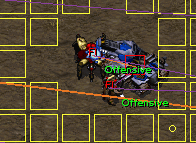
\includegraphics[width=4cm]{images/tank_cac.png}
\hspace{1cm}
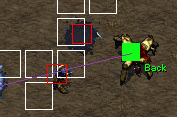
\includegraphics[width=4cm]{images/kiting.png}
\caption{Potential damage map (white squares for low potential damages, and yellow square for moderate potential damages). Left: we can see that the tank in siege mode (big blue unit with a red square on top) cannot shoot at close range and thus our units (in red) were attracted to the close safe zone. Right: the enemy units (blue, with red squares on top) are contact attack units and thus our unit (red, with a plain green square on top) is ``kiting'' (staying out of range): attacking and then retreating away (out of their range).}
\end{center}
\label{fig:potential_damage_map}
\end{figure}

\subsubsection{Repulsion/attraction}
For repulsion/attraction between units (allied or enemies), we could consider the instantaneous position of the units but it would lead to squeezing/expanding effects when moving large groups. Instead, we use their interpolated position at the time at which the unit that we move will be arrived in the direction we consider. In the right diagram in Figure~\ref{ fig:BayesianUnit_perceptions}, we want to move the unit in the center (\texttt{U}). There is an enemy (\texttt{E}) unit twice as fast as ours and an allied unit (\texttt{A}) three times as ours. When we consider moving in the direction just above us, we are on the interpolated position of unit \texttt{E} (we travel one case when they do two); when we consider moving in the direction directly on our right (East), we are on the interpolated position of unit \texttt{A}. 
We consider where the unit will be $\frac{\mathrm{dist}(unit, \vec{d_i})}{unit.speed}$ time later, but also its size (some units produce collisions in a smaller scale than our discretization).

\subsubsection{Objective}
The goals coming from the tactician model (see Fig.~\ref{fig:conceptMICRO}) are broken down into steps which gives objectives to each units. The way to incorporate the objective in the reactive behavior of our units is to add an attractive sensory input. This objective is a fixed direction $\vec{o}$ and we consider the probabilities of moving our unit in $n$ possible directions $\vec{d_1} \dots \vec{d_n}$ (in our StarCraft implementation: $n=25$ atomic directions). To decide the attractiveness of a given direction $\vec{d_i}$ with regard to the objective $\vec{o}$, we consider a weight which is proportional to the dot product $\vec{o} \cdot \vec{d_i}$, with a threshold minimum probability, as shown in Figure~\ref{fig:BayesianUnit_perceptions}.

\begin{figure}[h]
\begin{center}
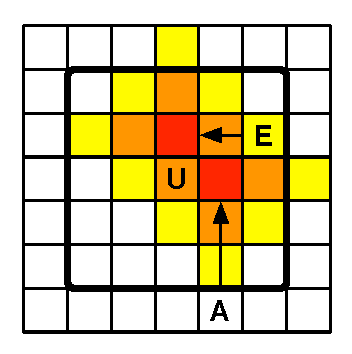
\includegraphics[width=4.5cm]{images/repulsion_units_interpolation.pdf}
\hspace{1cm}
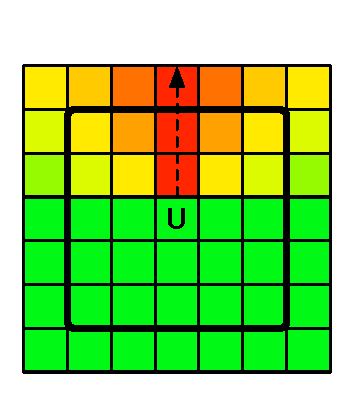
\includegraphics[width=4.5cm]{images/obj_Bayesian_units.pdf}
\caption{In both figures, the thick squares represents the boundaries of the 24 atomic directions (25 small squares with the current unit position) around the unit (\texttt{U}). Red is high probability, down to green low probability. Left: repulsion of the linear interpolation of the trajectories (here with uncertainty) of enemy unit (\texttt{E}) and allied unit (\texttt{A}), depending on their speed. Right: attraction of the objective (in direction of the dotted arrow) which is proportional to dot-product of the direction (square) considered, with a minimum threshold (in green).}
\label{fig:BayesianUnit_perceptions}
\end{center}
\end{figure}


\subsection{A Simple Unit}
\subsubsection{Greedy pragmatism}
Is staying alive better than killing an enemy unit? Is a large splash damage better than killing an enemy unit? Is it better to fire or move? In that event, where? Even if we could compute to the end of the fight and apply the same approach that we have for board games, how do we infer the best ``set of next moves'' for the enemy? %when the space of possible moves is so huge and the number of possible reasoning methods %(sacrifices and influences of other parts of the game for instance) 
%is bigger than for Chess? 
For enemy units, it would require exploring the tree of possible plans (intractable) whose we could at best only draw samples from \citep{UCT}. Even so, taking enemy minimax (to which depth?) moves for facts would assume that the enemy is also playing minimax (to the same depth) following exactly the same valuation rules as ours. Clearly, RTS \glos{micro} is more inclined to reactive planning than board games reasoning. That does not exclude having higher level (strategic and tactic) goals. In our model, they are fed to the unit as sensory inputs, that will have an influence on its behavior depending on the situation/state the unit is in. 
We should at least have a model for higher-level decisions of the enemy and account for uncertainty of moves that could be performed in this kind of minimax approach. So, as complete search through the min/max tree is intractable, we propose a first simple solution: have a greedy target selection heuristic leading the movements of units to benchmark our Bayesian model against. In this solution, each unit can be viewed as an effector, part of a multi-body (multi-effector) agent, grouped under a units group. 

\subsubsection{Targeting heuristic}
The idea behind the heuristic used for target selection is that units need to focus fire (which leads to less incoming damages if enemy units die faster) on units that do the most damages, have the less hit points, and take the most damages from their attack type. This can be achieved by using a data structure, shared by all our units engaged in the battle, that stores the damages corresponding to future allied attacks for each enemy units. Whenever a unit will fire on a enemy unit, it registers there the future damages on the enemy unit. As attacks are not all instantaneous and there are reload times, it helps focus firing greatly\footnote{The only degenerated case would be if all our units register their targets at once (and all the enemy units have the same priority) and it never happens (plus, units fire rates have a randomness factor).}. 
We also need a set of priority targets for each of our unit types that can be drawn from expert knowledge or learned (reinforcement learning) battling all unit types. A unit select its target among the most focus fired units with positive future hit point (current hit points minus registered damages), while prioritizing units from the priority set of its type. The units group can also impose its own priorities on enemy units (for instance to achieve a goal). The target selection heuristics is fully depicted in \ref{alg:targetselection} in the appendices.

\subsubsection{Fight behavior}
\label{sec:HOAI}
Based on this targeting heuristic, we design a very simple \glos{FSM} based unit as shown in Figure~\ref{fig:fight_FSM} and Algorithm~\ref{alg:fight_FSM}: when the unit is not firing, it will either flee damages if it has taken too much damages and/or if the differential of damages is too strong, or move to be better positioned in the fight (which may include staying where it is). In this simple unit, the \textit{flee()} function just tries to move the unit in the direction of the biggest damages gradient (towards lower potential damages zones). The \textit{fightMove()} function tries to position the units better: in range of its priority target, so that if the priority target is out of reach, the behavior will look like: ``try to fire on target in range, if it cannot (reloading or no target in range), move towards priority target''. As everything is driven by the firing heuristic (that we will also use for our Bayesian unit), we call this AI the Heuristic Only AI (HOAI).

\begin{figure}[h]
\begin{algorithmic}
\Function{move}{$prio\_t, \nabla dmg$}
\If {$needFlee()$}
    \State {$flee(\nabla dmg)$}
\Else
    \State {$fightMove(prio\_t)$}
\EndIf
\EndFunction

\Function{fight}{}
\State $(target, prio\_target) = selectTarget()$
\If {$reloaded$}
    \If {$inRange(prio\_target)$}
        \State {$attack(prio\_target)$}
    \ElsIf {$inRange(target)$}
        \State {$attack(target)$}
    \Else
        \State {$move(prio\_target, damage\_gradient)$}
    \EndIf
\Else
    \State {$move(prio\_target, damage\_gradient)$}
\EndIf
\EndFunction
\end{algorithmic}
\caption{Fight behavior FSM for micro-managing units.}
\label{alg:fight_FSM}
\end{figure}

\begin{figure}[h]
\begin{center}
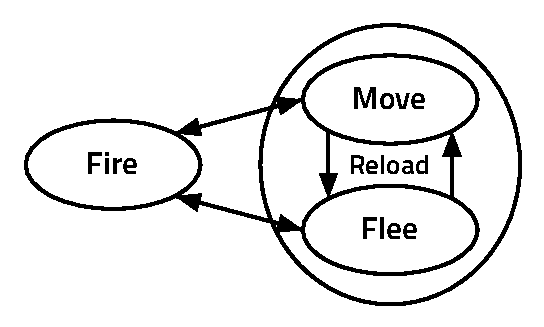
\includegraphics[width=5.5cm]{images/simple_unit_fight_FSM.pdf}
\end{center}
\caption{Fight FSM of a simple unit model: Heuristic Only AI (HOAI), which will serve as a baseline for benchmarks.}
\label{fig:fight_FSM}
\end{figure}


\subsection{Units Group}

\label{sec:unitsgroup}
The units group (\texttt{UnitsGroup}, see Fig.~\ref{fig:conceptMICRO}) makes the shared \textit{future damage} data structure available to all units taking part in a fight. Units control is not limited to fight. As it is adversarial, it is perhaps the hardest task, but units control problems comprehends efficient team maneuvering and other behaviors such as scouting or staying in position (formation). The units group structure helps for all that: it decides of the modes in which the unit has to be. We implemented 4 modes in our Bayesian unit (see Fig.~\ref{fig:unit_HFSM}): \textit{fight, move, scout, inposition}. When given a task, also named goal, by the tactician model (see Fig.~\ref{conceptMICRO}), the units group has to transform the task objective into sensory inputs for the units. 
\begin{itemize}
    \item In \textit{scout} mode, the (often quick and low hit points) unit avoids danger by modifying locally its pathfinding-based, objectives oriented route to avoid damages.
    \item In \textit{move} mode, the objective is extracted for the pathfinder output: it consists in key waypoints near the units. When moving by flocking, our unit moves are influenced by other near allied units that repulse or attract it depending on its distance to the interpolation of the allied unit. It allows our units to move more efficiently by not splitting around obstacles and colliding less. As it causes other problems, we do not use the flocking behavior in full competitive games.
    \item In the \textit{inposition} mode, the objective is the final unit formation position. The unit can be ``pushed'' by other units wanting to pass through. This is useful at a tactical level to do a wall of units that our units can traverse but the opponent's cannot. Basically, there is an attraction to the position of the unit and a stronger repulsion of the interpolation of movements of allied units.
    \item In \textit{fight} mode, our unit will follow the damages gradient to smart positions, for instance close to tanks (they cannot fire too close to their position) or far from too much contact units if our unit can attack with range (something called ``kiting''). Our unit moves are also influenced by its priority targets, its goal/objective (go through a choke, flee, etc.) and other units. The objective depends of the confidence of the units group in the outcome of the battle:
\begin{itemize}
    \item If the units group is outnumbered (in adjusted strength) and the task is not a suicidal one, the units group will ``fall back'' and give objectives towards retreat. 
    \item If the fight is even or manageable, the units group will not give any objective to units, which will set their own objectives either to their priority targets in \textit{fightMove()} or towards fleeing damages (towards highest potential damages gradient) in \textit{flee()}.
    \item If the units group is very confident in winning the fight, the objectives sensory inputs of the units will be set at the task objectives waypoints (from the pathfinder).
\end{itemize}
\end{itemize} 

\section{A Bayesian Model for Units Control}

\label{sec:bayesianunit}
\subsection{Bayesian Unit}

We use Bayesian programming as an alternative to logic, transforming incompleteness of knowledge about the world into uncertainty. In the case of units management, we have mainly \textit{intensional} uncertainty. Instead of asking questions like: where are other units going to be 10 frames later? Our model is based on rough estimations that are not taken as ground facts. Knowing the answer to these questions would require for our own (allied) units to communicate a lot and to stick to their plan (which does not allow for quick reaction nor adaptation). 

We propose to model units as sensory-motor robots described within the Bayesian robot programming framework \citep{Lebeltel04}. A Bayesian model uses and reasons on distributions instead of predicates, which deals directly with uncertainty. %Basically, a Bayesian unit will be attracted or repulsed by its sensory inputs. 
Our Bayesian units are simple hierarchical finite states machines (states can be seen as modes) that can scout, fight and move (see Figure~\ref{fig:unit_HFSM}). Each unit type has a reload rate and attack duration, so their fight mode will be as depicted in Figure~\ref{fig:fight_FSM} and Algorithm~\ref{alg:fight_FSM}. The difference between our simple HOAI presented above and Bayesian units are in \textit{flee()} and \textit{fightMove()} functions.
\begin{figure}[h]
\begin{center}
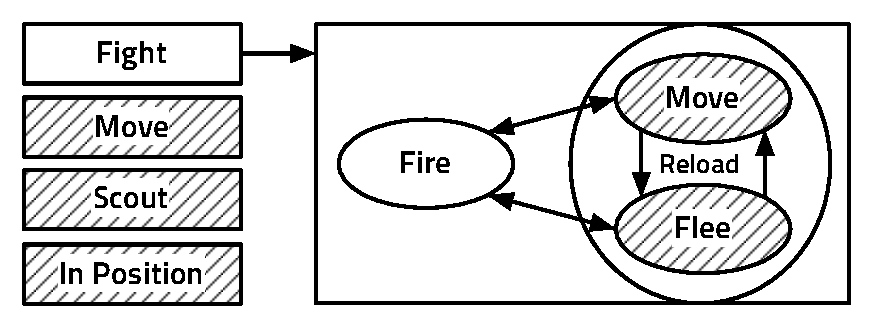
\includegraphics[width=7cm]{images/unit_HFSM2.pdf}
\end{center}
\caption{Bayesian unit modal FSM (\glos{HFSM}), detail on the fight mode. Stripped modes are Bayesian.}
\label{fig:unit_HFSM}
\end{figure}

The unit needs to determine where to go when fleeing and moving during a fight, with regard to its target and the attacking enemies, while avoiding collisions (which results in blocked units and time lost) as much as possible. \textbf{We now present the Bayesian program used for \textit{flee()}, \textit{fightMove()}, and while scouting}, which differ only by what is inputed as objective:
\subsubsection{Variables}
\begin{itemize}
\item $Dir_{i \in \llbracket 1 \dots n\rrbracket } \in \{True, False\}$: at least one variable for each atomic direction the unit can go to. $\PP(Dir_i = True) = 1$ means that the unit will certainly go in direction $i$ ($\Leftrightarrow \vec{d_i}$). For example, in StarCraft we use the 24 atomic directions (48 for the smallest and fast units as we use a proportional scale) plus the current unit position (stay where it is) as shown in Figure~\ref{fig:sc_fight}. %We could use one variable with 24 directions, the approach would be the same. %%% Note that $i \in \llbracket 1 \dots n\rrbracket \Leftrightarrow \mathbf{D}[i] \in \mathbf{D}$.

\item $Obj_{i \in \llbracket 1 \dots n\rrbracket } \in \{True, False\}$: adequacy of direction $i$ with the objective (given by a higher rank model). In our StarCraft AI, we use the scalar product between the direction $i$ and the objective vector (output of the pathfinding) with a minimum value ($0.3$ in \textit{move} mode for instance) so that the probability to go in a given direction is proportional to its alignment with the objective.
\begin{itemize}
    \item For \textit{flee()}, the objective is set in the direction which flees the potential damage gradient (corresponding to the unit type: ground or air).
    \item For \textit{fightMove()}, the objective is set (by the units group) either to retreat, to fight freely or to march aggressively towards the goal (see \ref{sec:unitsgroup}).
    \item For the \textit{scout} behavior, the objective ($\vec{o}$) is set to the next pathfinder waypoint.
\end{itemize}

\item $Dmg_{i \in \llbracket 1 \dots n\rrbracket } \in \{no, low, medium, high\}$: potential damage value in direction $i$, relative to the unit base health points, in direction $i$. In our StarCraft AI, this is directly drawn from two constantly updated potential damage maps (air, ground). %For instance, it allows our scouting units to avoid potential attacks as much as possible.

\item $A_{i \in \llbracket 1 \dots n\rrbracket } \in \{free, small, big\}$: occupation of the direction $i$ by an allied unit. The model can effectively use many values (other than ``occupied/free'') because directions may be multi-scale (for instance we indexed the scale on the size of the unit) and, in the end, small and/or fast units have a much smaller footprint, collision wise, than big and/or slow. In our AI, instead of direct positions of allied units, we used their (linear) interpolation $\frac{\mathrm{dist}(unit, \vec{d_i})}{unit.speed}$ (time it takes the unit to go to $\vec{d_i}$) 
frames later (to avoid squeezing/expansion).

\item $E_{i \in \llbracket 1 \dots n\rrbracket } \in \{free, small, big\}$: occupation of the direction $i$ by an enemy unit. As above.

\item $Occ_{i \in \llbracket 1 \dots n\rrbracket } \in \{free, building, staticterrain\}$%(this could have been 2 variables or we could omit static terrain but we stay as general as possible): 
: Occupied, repulsive effect of buildings and terrain (cliffs, water, walls).
\end{itemize}

There is basically one set of (sensory) variables per perception in addition to the $Dir_i$ values. 

\subsubsection{Decomposition}

The joint distribution ($JD$) over these variables is a specific kind of fusion called inverse programming \citep{LeHy04}. The sensory variables are considered conditionally independent knowing the actions, contrary to standard naive Bayesian fusion, in which the sensory variables are considered independent knowing the phenomenon.
\begin{eqnarray}
&& \PP(Dir_{1:n}, Obj_{1:n}, Dmg_{1:n}, A_{1:n}, E_{1:n}, Occ_{1:n})\\
& = & JD = \prod_{i=1}^{n} \PP(Dir_i) \PP(Obj_i | Dir_i) \\
                    && \PP(Dmg_i | Dir_i) \PP(A_i | Dir_i) \\
                    && \PP(E_i | Dir_i) \PP(Occ_i | Dir_i)
\end{eqnarray}
We assume that the $i$ directions are independent depending on the action because dependency is already encoded in (all) sensory inputs. 

\subsubsection{Forms}

\begin{itemize}
\item $\PP(Dir_i)$ prior on directions, unknown, so unspecified/uniform over all $i$. $\PP(dir_i) = 0.5$.

\item $\PP(Obj_i | Dir_i)$ for instance, ``probability that this direction is the objective knowing that we go there'' $\PP(obj_i | dir_i) = threshold + (1.0-threshold)\times \mathrm{max}(0, vec{o} \cdot \vec{d_i})$. %$\PP(Obj_i = T | Dir_i = T)$ is very high (close to one) when rushing towards an objective, whereas it is far less important when fleeing. 
We could have different $thresholds$ depending on the mode, this was not the case in our hand-specified tables: $threshold = 0.3$. The right diagram on Figure~\ref{fig:BayesianUnit_perceptions} shows $\PP(Obj_i|Dir_i)$ for each for the possible directions (inside the thick big square boundaries of atomic directions) with red being higher probabilities.

\item $\PP(Dmg_i | Dir_i)$ probability of damages values in direction $i$ knowing this is the direction that we are headed to. $\PP(Dmg_i = high | Dir_i = T)$ has to be small in many cases for the unit to avoid going to positions it could be killed instantly. Probability table:\\
\begin{center}
\begin{tabular}{|l|c|c|}
\hline
$Dmg_i$ & $dir_i$ & $\bar{dir_i}$ \\
\hline
no & 0.9 & 0.25 \\
low & 0.06 & 0.25 \\
medium & 0.03 & 0.25 \\
high & 0.01 & 0.25 \\
\hline
\end{tabular}
\end{center}

\item $\PP(A_i | Dir_i)$ probability that there is an ally in direction $I$ knowing this is the unit direction. It is used to avoid collisions by not going where allied units could be in the near future. Probability table:\\
\begin{center}
\begin{tabular}{|l|c|c|}
\hline
$A_i$ & $dir_i$ & $\bar{dir_i}$ \\
\hline
free & 0.9 & 0.333 \\
small & 0.066 & 0.333 \\
big & 0.033 & 0.333 \\
\hline
\end{tabular}
\end{center}
 

\item $\PP(E_i | Dir_i)$ same explanation and use as above but with enemy units, it can have different parameters as we may want to be stucking enemy units, or avoid them (mostly depending on the unit type). In a repulsive setting (what we mostly want), the left diagram in Figure~\ref{fig:BayesianUnit_perceptions} can be seen as $\PP(A_i,E_i | \bar{Dir_i})$ if red corresponds to high probabilities ($\PP(A_i,E_i|Dir_i)$ if red corresponds to lower probabilities). In our hand-specified implementation, for \textit{flee()} and \textit{fightMove()}, this is the same probability table as above (for $\PP(A_i | Dir_i)$).

\item $\PP(Occ_i | Dir_i)$ probability table that there is a blocking building or terrain element is some direction, knowing this is the unit direction, $\PP(Occ_i = Static | Dir_i = T)$ will be very low, whereas $\PP(Occ_i = Building | Dir_i = T)$ will also be very low but triggers building attack (and destruction) when there are no other issues.
Probability table:\\
\begin{center}
\begin{tabular}{|l|c|c|}
\hline
$Occ_i$ & $dir_i$ & $\bar{dir_i}$ \\
\hline
free & 0.999899 & 0.333 \\
building & 0.001 & 0.333 \\
static & 0.000001 & 0.333 \\
\hline
\end{tabular}
\end{center}

\end{itemize}



\subsubsection{Identification}

Parameters and probability tables can be learned through reinforcement learning \citep{Sutton,Asmuth09} by setting up different and pertinent scenarii and search for the set of parameters that maximizes a reward function (more about that in the discussion). In our current implementation, the parameters and probability table values are hand specified.

\subsubsection{Question}

When in \textit{fightMove()} and \textit{flee()}, the unit asks:
\begin{equation}
\PP(Dir_{1:n} | Obj_{1:n}, Dmg_{1:n}, A_{1:n}, E_{1:n}, Occ_{1:n})
\end{equation}

From there, the unit can either go in the most probable $Dir_i$ or sample through them. We describe the effect of this choice in the next section (and in Fig.~\ref{fig:BayesianUnitChoice}). A simple Bayesian fusion from 3 sensory inputs is shown in Figure~\ref{fig:BayesianUnitExample}, in which the final distribution on $Dir$ peaks at places avoiding damages and collisions while pointing towards the goal. Here follows the full Bayesian program of the model (\ref{bp:BayesianUnit_fightmove}):

\begin{figure}[h]
\begin{center}
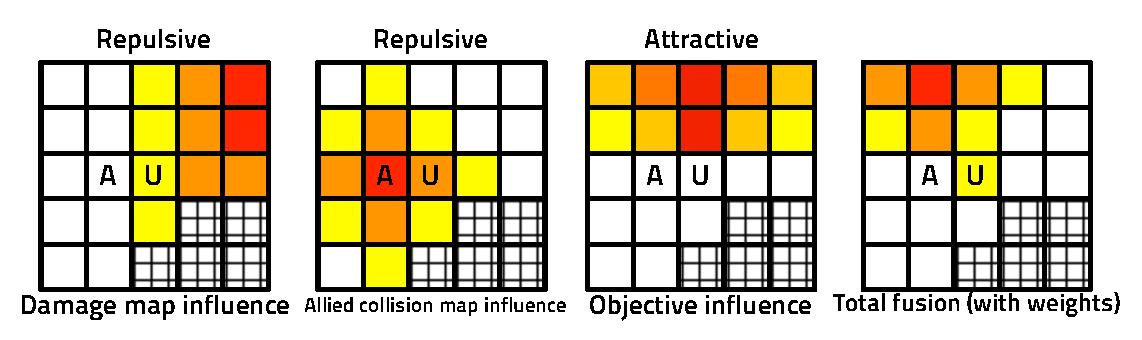
\includegraphics[width=0.89\columnwidth]{images/example_BayesianUnit.pdf}
\end{center}
\caption{Simple example of Bayesian fusion from 3 sensory inputs (damages and collisions avoidance, goal attraction). The grid pattern represents statically occupied terrain, the unit we control is in \texttt{U}, an allied unit is in \texttt{A}. The result is displayed on the rightmost image.}
\label{fig:BayesianUnitExample}
\end{figure}

\begin{figure}[!h]
\begin{eqnarray*}
\begin{sideways}\parbox{35mm}{\hspace{-1.3cm}Bayesian program}\end{sideways}
\begin{cases}
\begin{sideways}\parbox{15mm}{\hspace{-0.8cm}Description}\end{sideways}
    \begin{cases}
\begin{sideways}\parbox{18mm}{\hspace{-1.1cm}Specification ($\pi$)}\end{sideways}
        \begin{cases}
        Variables\\
Dir_{1:n}, Obj_{1:n}, Dmg_{1:n}, A_{1:n}, E_{1:n}, Occ_{1:n} \\
        Decomposition\\
 \PP(Dir_{1:n}, Obj_{1:n}, Dmg_{1:n}, A_{1:n}, E_{1:n}, Occ_{1:n}) =  \prod_{i=1}^{n} \big[ \PP(Dir_i) \\
 \PP(Obj_i | Dir_i) \PP(Dmg_i | Dir_i) \PP(A_i | Dir_i) \PP(E_i | Dir_i) \PP(Occ_i | Dir_i)\big]\\
        Forms\\
\PP(Dir_i): \mathrm{prior\ on\ directions\ (crossing\ policy)} \\
\PP(XYZ_i | Dir_i):\ \mathrm{probability\ tables}\\
        \end{cases}\\
    Identification\ (using\ \delta)\\
\mathrm{reinforcement\ learning\ or\ hand\ specified\ (or\ distribs.\ parameters\ optimization)}
    \end{cases}\\
Question\\
 \mathrm{fight moving/fleeing/scouting:}\ \ \PP(Dir_{1:n} | Obj_{1:n}, Dmg_{1:n}, A_{1:n}, E_{1:n}, Occ_{1:n})\\
%%%  \mathrm{fleeing:}\ \  \PP(Dir_{1:n} | Obj_{1:n}, Dmg_{1:n}, A_{1:n}, E_{1:n}, Occ_{1:n})\\
%%%  \mathrm{flocking:}\ \  \PP(Dir_{1:n} | Obj_{1:n}, Dmg_{1:n}, A_{1:n}, E_{1:n}, Occ_{1:n}, Att_{1:n,1:m})\\
\end{cases}
\end{eqnarray*}
\caption{Bayesian program of \textit{flee()}, \textit{fightMove()} and the \textit{scouting} behaviors.}
\label{bp:BayesianUnit_fightmove}
\end{figure}

There are additional variables for specific modes/behaviors, also probability tables may be different.

\subsubsection{Move}

\noindent\textit{Without flocking}\\
When moving without flocking (trying to maintain some form of group cohesion), the model is even simpler. The objective ($\vec{o}$) is set to a path waypoint. The potential damage map is dropped from the $JD$, the question is:
\begin{equation}
\PP(Dir_{1:n} | Obj_{1:n}, A_{1:n}, E_{1:n}, Occ_{1:n})
\end{equation}

\noindent\textit{With flocking}\\
%To produce a \textit{flocking} behavior while moving, with $m$ units, we introduce another set of variables: $Att_{i \in \llbracket 0 \dots n\rrbracket, j \in \llbracket 0 \dots m \rrbracket} \in \{too\_close, near, far, too\_far\}$\footnote{the discrete levels could be replaced by the distance and $\PP(Att_{i,j}|Dir_i)$ could use a $Beta(\alpha, \beta)$ distribution with $\beta > \alpha > 1$.}, allied units attractions and repulsions. 
%Different than $A_i$, the $JD$ would become $JD \times \Pi_{i=1}^{n} \Pi_{j=1}^{m} \PP(Att_{i,j} | Dir_i)$, where $\PP(Att_{i,j} | Dir_i)$\footnote{Changing for $\PP(Att_i|Dir_i)P(Dir_i)$ for $\PP(Dir_i|Att_i)$ may be easier to reason about.} is a probability table for flocking: a too close unit $j$ will repel the Bayesian unit ($\PP(Att_{i,j} | Dir_i) < mean$) whereas another unit $j$ will attract depending on its distance (and possibly, leadership).
To produce a \textit{flocking} behavior while moving, we introduce another set of variables: $Att_{i \in \llbracket 1 \dots n\rrbracket} \in \{True,False\}$, allied units attractions (or not) in direction $i$.

A flocking behavior \citep{Reynolds_1999} requires:
\begin{itemize}
    \item Separation: avoid collisions, short range repulsion,
    \item Alignment: align direction with neighbours,
    \item Cohesion: steer towards average position of neighbours.
\end{itemize}
Separation is dealt with by $\PP(A_i|Dir_i)$ already. As we use interpolations of units at the time at which our unit will be arrived at the $Dir_i$ under consideration, being attracted by $Att_i$ gives cohesion as well as some form of alignment. It is not strictly the same as having the same direction and seems to fare better is complex terrain. We remind the reader that flocking was derived from birds flocks and fish schools behaviors: in both cases there is a lot of free/empty space.

A $\vec{a}$ vector is constructed as the weighted sum of neighbour\footnote{The devil is in the details, if one considers a too small neighbourhood, there is very rarely emergence of the flocking behavior, whereas if one considers a too large neighbourhood, units can get in directions which are stucking them with terrain. A pragmatic solution is to use a large neighbourhood with a decreasing weight (for increasing distance) for each unit of the neighbourhood.} allied units. Then $\PP(Att_i|Dir_i)$%\footnote{Changing for $\PP(Att_i|Dir_i)P(Dir_i)$ for $\PP(Dir_i|Att_i)$, with $Att_i$ being the distance, may be easier to reason about.}
 for all $i$ directions is constructed as for the objective influence ($\PP(Obj_i|Dir_i)$) by taking the dot product $\vec{a} \cdot \vec{d_i}$ with a minimum threshold (we used 0.3, so that the flocking effect is as strong as objective attraction):
$$\PP(att_i|dir_i) = threshold + (1.0-threshold)\times \mathrm{max}(0, \vec{a} \cdot \vec{d_i})$$

The $JD$ becomes $JD \times \Pi_{i=1}^{n} \PP(Att_{i} | Dir_i)$.
%%% \begin{center}
%%% \begin{tabular}{|l|c|c|}
%%% \hline
%%% $Att_{i,j}$ & $dir_i$ & $\bar{dir_i}$ \\
%%% \hline
%%% close & 0.4 & 0.5 \\
%%% far & 0.5 & 0.05 \\
%%% too\_far & 0.1 & 0.9 \\
%%% \hline
%%% \end{tabular}
%%% \end{center}

\begin{figure}[h]
\begin{eqnarray*}
\begin{sideways}\parbox{35mm}{\hspace{-1.3cm}Bayesian program}\end{sideways}
\begin{cases}
\begin{sideways}\parbox{15mm}{\hspace{-0.8cm}Description}\end{sideways}
    \begin{cases}
\begin{sideways}\parbox{18mm}{\hspace{-1.1cm}Specification ($\pi$)}\end{sideways}
        \begin{cases}
        Variables\\
Dir_{1:n}, Obj_{1:n}, Att_{1:n}, A_{1:n}, E_{1:n}, Occ_{1:n} \\
%Dir_{1:n}, Obj_{1:n}, Att_{1:n,1:m}, A_{1:n}, E_{1:n}, Occ_{1:n} \\
        Decomposition\\
 \PP(Dir_{1:n}, Obj_{1:n}, Att_{1:n}, A_{1:n}, E_{1:n}, Occ_{1:n}) =  \prod_{i=1}^{n} \big[ \PP(Dir_i) \\
% \PP(Dir_{1:n}, Obj_{1:n}, Att_{1:n,1:m}, A_{1:n}, E_{1:n}, Occ_{1:n}) =  \prod_{i=1}^{n} \big[ \PP(Dir_i) \\
 \PP(Obj_i | Dir_i) \PP(A_i | Dir_i) \PP(E_i | Dir_i) \PP(Occ_i | Dir_i)
\PP(Att_{i} | Dir_i)
%\prod_{j=1}^{m} \PP(Att_{i,j} | Dir_i)
\big]\\
        Forms\\
\PP(Dir_i): \mathrm{prior\ on\ directions\ (crossing\ policy)} \\
\PP(XYZ_i | Dir_i):\ \mathrm{probability\ tables}\\
        \end{cases}\\
    Identification\ (using\ \delta)\\
\mathrm{learning\ or\ hand\ specified}\\
    \end{cases}\\
Question\\
 \mathrm{without\ flocking\ (no\ }Att_{1:n}\ \mathrm{variables):}\ \  \PP(Dir_{1:n} | Obj_{1:n}, A_{1:n}, E_{1:n}, Occ_{1:n})\\
 \mathrm{with\ flocking:}\ \  \PP(Dir_{1:n} | Obj_{1:n}, A_{1:n}, E_{1:n}, Occ_{1:n}, Att_{1:n})\\
% \mathrm{flocking:}\ \  \PP(Dir_{1:n} | Obj_{1:n}, A_{1:n}, E_{1:n}, Occ_{1:n}, Att_{1:n,1:m})\\
\end{cases}
\end{eqnarray*}
\caption{Bayesian program of the \textit{move} behavior without and with flocking.}
\label{bp:BayesianUnit_move}
\end{figure}


\subsubsection{In position}

%\item $Prio_{i \in \llbracket 1 \dots n\rrbracket } \in \{True, False\}$: combined effect of the priority targets that attract the unit while in fight ($fightMove()$). The $JD$ is modified as $JD \times \Pi_{i=1}^{n} \PP(Prio_i | Dir_i)$, where $\PP(Prio_i | Dir_i)$ is a probability table, that corresponds to the attraction of a priority (maybe out of range) target in this direction. This is efficient to be able to target casters or long range units for instance.
The \textit{inposition} mode corresponds to when some units are at the place they should be (no new objective to reach) and not fighting. This happens when some units arrived at their formation end positions and they are waiting for other (allied) units of their group, or when units are sitting (in defense) at some tactical point, like in front of a base for instance. The particularity of this mode is that the objective is set to the current unit position and it will be updated to always point to this ``final formation position'' as long as the unit is in this mode. This is useful so that units which are arriving to the formation can go through each others and not get stuck. Figure~\ref{fig:squaretraversal} shows the effect of using this mode: the big unit (Archon) goes through a square formation of the other units (Dragoons) which are in \textit{inposition} mode. What happens is an emerging phenomenon: the first (leftmost) units of the square get repulsed by the interpolated position of the dragoon, so they move themselves out of its trajectory. By moving, they repulse the second and then third line of the formation, the chain repulsion reaction makes a path for the big unit to pass through the formation. Once this unit path is no longer colliding, the attraction of units for their objective (their formation position) takes them back to their initial positions.

\begin{figure}[h]
\begin{center}
\begin{tabular}{cc}
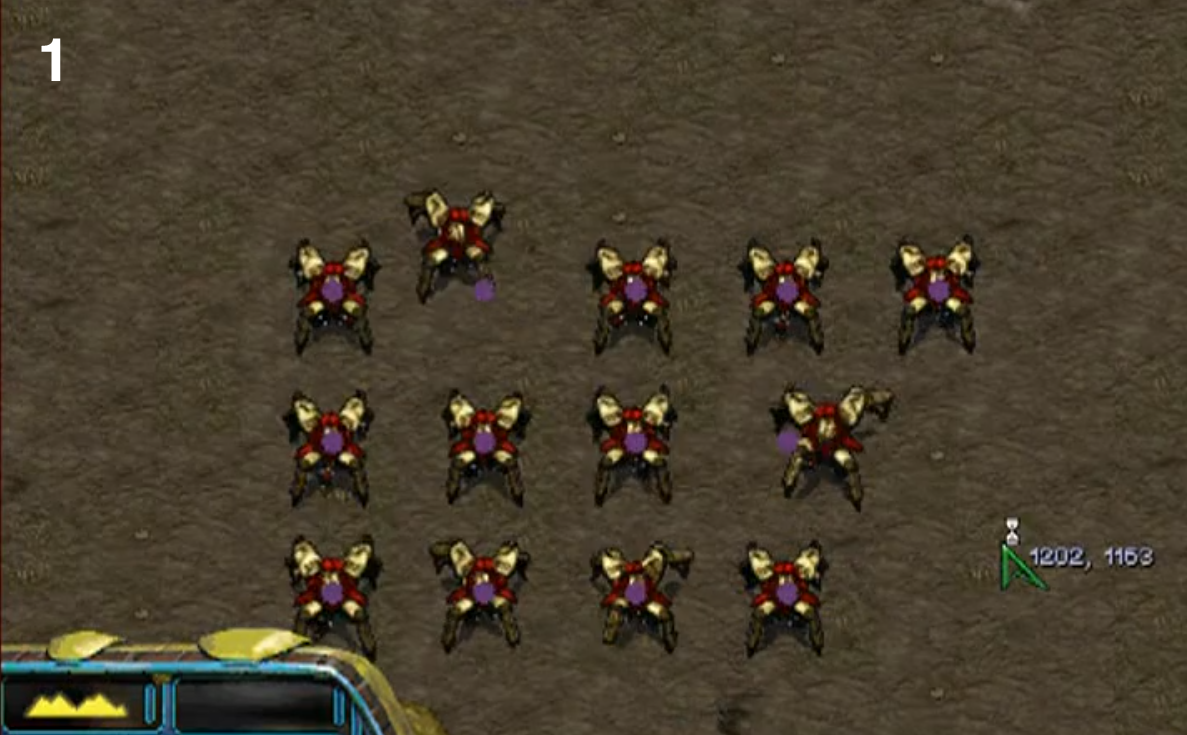
\includegraphics[width=0.47\columnwidth]{images/square_traversal_1.png} & 
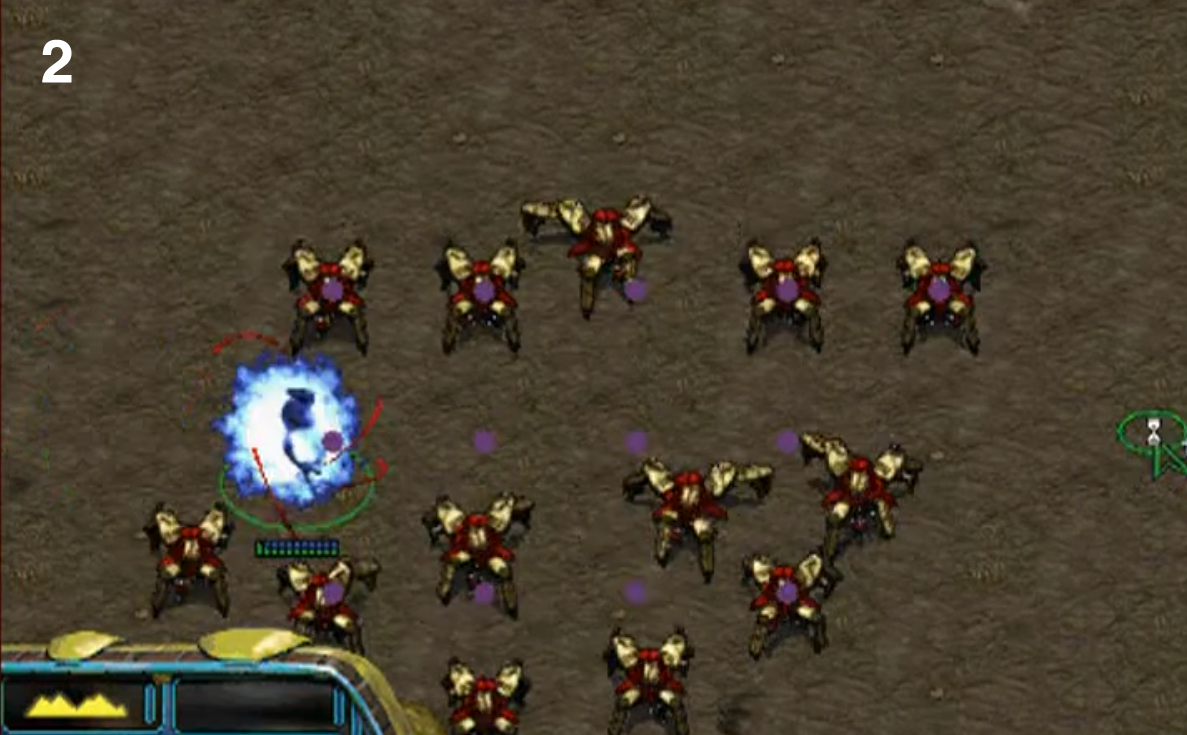
\includegraphics[width=0.47\columnwidth]{images/square_traversal_2.png} \\
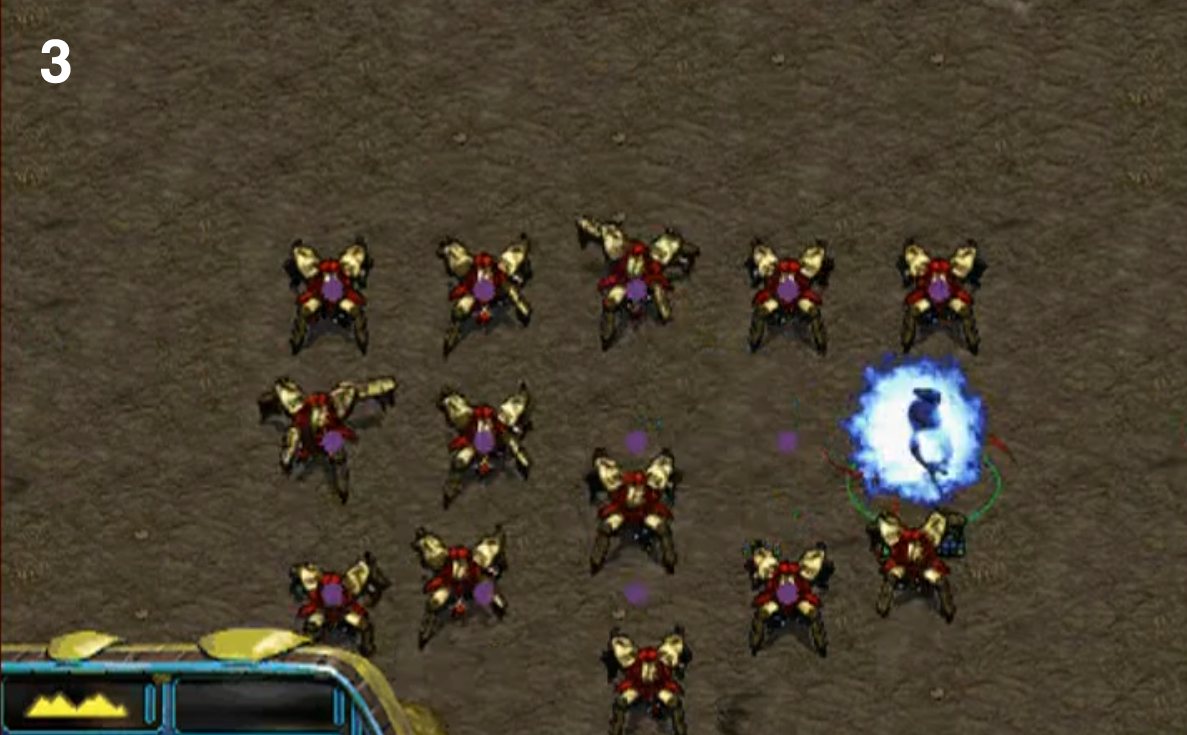
\includegraphics[width=0.47\columnwidth]{images/square_traversal_3.png} & 
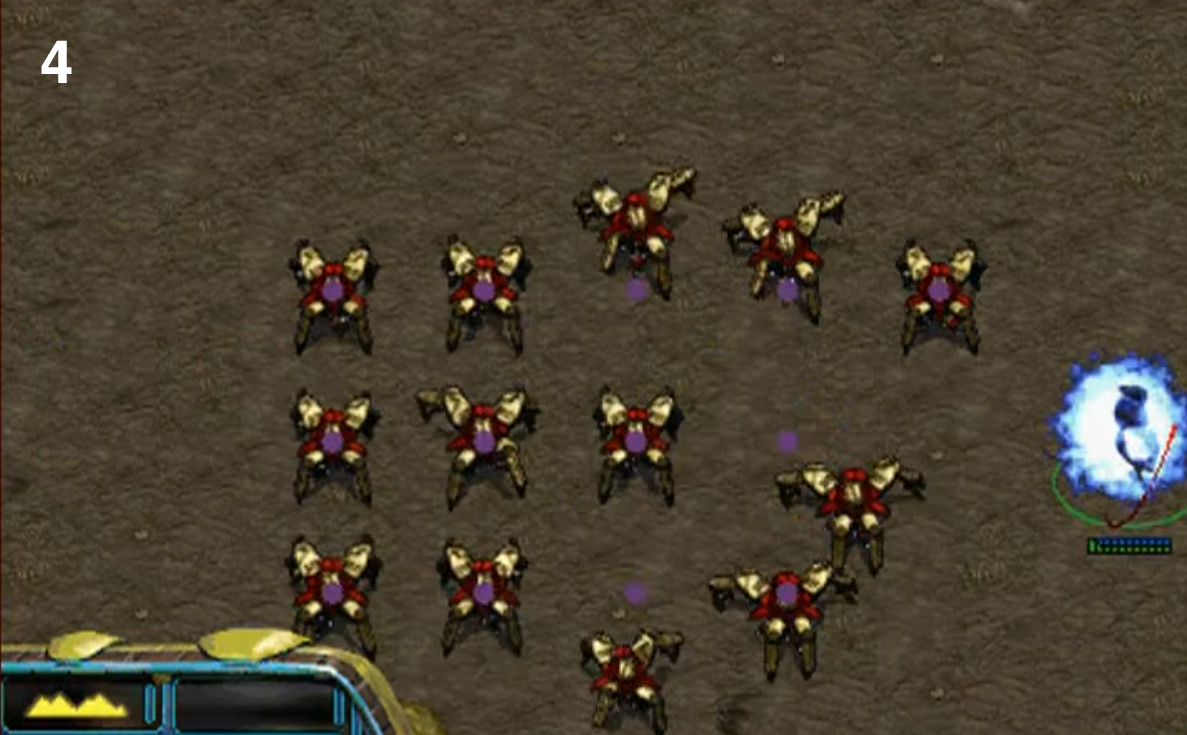
\includegraphics[width=0.47\columnwidth]{images/square_traversal_4.png} \\
\end{tabular}
\caption{Sequence of traversal of an Archon (big blue unit which is circled in green) through a square formation of Dragoons (four legged red units) in \textit{inposition} mode.}
\label{fig:squaretraversal}
\end{center}
\end{figure}


\section{Results on StarCraft}

Our implementation\footnote{\textsc{BroodwarBotQ}, code and releases: \url{http://github.com/SnippyHolloW/BroodwarBotQ}} (BSD licensed) uses BWAPI\footnote{BWAPI: \url{http://code.google.com/p/bwapi/}} to get information from and to control StarCraft. 

\subsection{Experiments}

We produced three different AI to run experiments with, along with the original AI (OAI) from StarCraft:
\begin{itemize}
\item Heuristic only AI (HOAI), as described above (\ref{sec:HOAI}): this AI shares the target selection heuristic with our Bayesian AI models and will be used as a baseline reference to avoid the bias due to the target selection heuristic.
\item Bayesian AI picking best (BAIPB): this AI follows the model of section~\ref{sec:bayesianunit} and selects the most probable $Dir_i$ as movement. 
\item Bayesian AI sampling (BAIS): this AI follows the model of section~\ref{sec:bayesianunit} and samples through $Dir_i$ according to their probability (i.e. it samples a direction in the $Dir$ distribution).
\end{itemize}

The experiments consisted in having the AIs fight against each others on a micro-management scenario with mirror matches of 12 and 36 ranged ground units (Dragoons). In the 12 units setup, the unit movements during the battle is easier (less collision probability) than in the 36 units setup. We instantiate only the army manager (no economy in this special scenarii/maps), one units group manager and as many Bayesian units as there are units provided to us in the scenario. The results are presented in Table~\ref{tab:win_ratios}.

\definecolor{grey}{rgb}{0.7,0.7,0.7}
\begin{table}[h]
\begin{center}
\begin{tabular}{|l|c|c|c|c|}
\hline
12 units & OAI & HOAI & BAIPB & BAIS \\
\hline
OAI & (50\%) & & & \\
HOAI & 59\% & (50\%) & & \\
BAIPB & 93\% & 97\% & (50\%) & \\
BAIS & 93\% & 95\% & 76\% & (50\%)\\
\hline
\end{tabular}
\ifthenelse{\equal{\myprintformat}{true}}{
\\
}{}
\begin{tabular}{|l|c|c|c|c|}
\hline
36 units & OAI & HOAI & BAIPB & BAIS \\
\hline
OAI & (50\%) & & & \\
HOAI & 46\% & (50\%) & & \\
BAIPB & 91\% & 89\% & (50\%) & \\
BAIS & 97\% & 94\% & 97\% & (50\%)\\
\hline
\end{tabular}
\end{center}
% BAIPB+Heuristics flee/fightmove 12 goons vs OAI 94/100
% BAIPB+Heuristics flee/fightmove 36 goons vs OAI 95/100
% pure BAIPB (fightMove only on ``potential fields'') 12 goons vs OAI 51/33
% pure BAIPB (fightMove only on ``potential fields'') 36 goons vs OAI 10/16
%%%\caption{Win ratios over at least 200 battles of the Original AI (OAI), Heuristic Only AI (HOAI), Bayesian AI Pick Best (BAIPB) and Bayesian AI Sample (BAIS) in two mirror setups: 12 and 36 ranged units. Read line vs column: for instance HOAI won 59\% of its matches against OAI in the 12 units setup. Note: The average amount of units left at the end of battles is proportional to the percentage of wins.}
\ifthenelse{\equal{\myprintformat}{true}}{
\caption{Win ratios over at least 200 battles of OAI, HOAI, BAIPB and BAIS in two mirror setups: 12 and 36 ranged units. 
Top: 12 units (12 vs 12) setup. Bottom: 36 units (36 vs 36) setup. Read line vs column: for instance HOAI won 59\% of its matches against OAI in the 12 units setup.}}{
\caption{Win ratios over at least 200 battles of OAI, HOAI, BAIPB and BAIS in two mirror setups: 12 and 36 ranged units. 
Left: 12 units (12 vs 12) setup. Right: 36 units (36 vs 36) setup. Read line vs column: for instance HOAI won 59\% of its matches against OAI in the 12 units setup.} %Note: The average amount of units left at the end of battles is grossly proportional to the percentage of wins.}
}
\label{tab:win_ratios}
\end{table}

These results show that our heuristic (HAOI) is comparable to the original AI (OAI), perhaps a little better, but induces more collisions as we can see its performance diminish a lot in the 36 units setup vs OAI. For Bayesian units, the ``pick best'' (BAIPB) direction policy is very effective when battling with few units (and few movements because of static enemy units) as proved against OAI and HOAI, but its effectiveness decreases when the number of units increases: all units are competing for the best directions (to $flee()$ or $fightMove()$ in) and they collide. The sampling policy (BAIS) has way better results in large armies, and significantly better results in the 12 units vs BAIPB. BAIPB may lead our units to move inside the ``enemy zone'' a lot more to chase priority targets (in \textit{fightMove()}) and collide with enemy units or get kill. Sampling entails that the competition for the best directions is distributed among all the ``bests to good'' positions, from the units point of view. We illustrate this effect in Figure~\ref{fig:BayesianUnitChoice}: the units (on the right of the figure) have good reasons (combinations of sensory inputs, for instance of the damage map) to flee on the left, and there may be a peak of ``best position to be at''. AS they have not moved yet, they do not have interpolation of positions which will collide, so they are not repulsing each other at this position, all go together and collide. Sampling would, on average, provide a collision free solution here.
\begin{figure}[h]
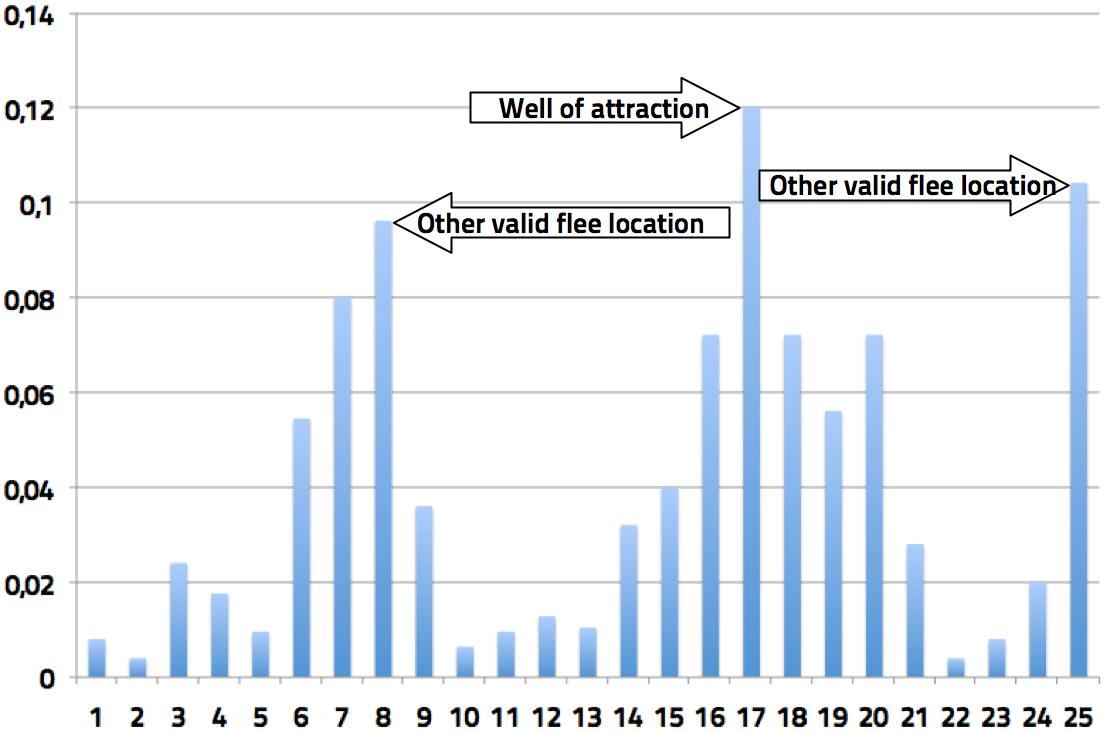
\includegraphics[width=0.75\columnwidth]{images/distDir.png}
\hspace{0.05\columnwidth}
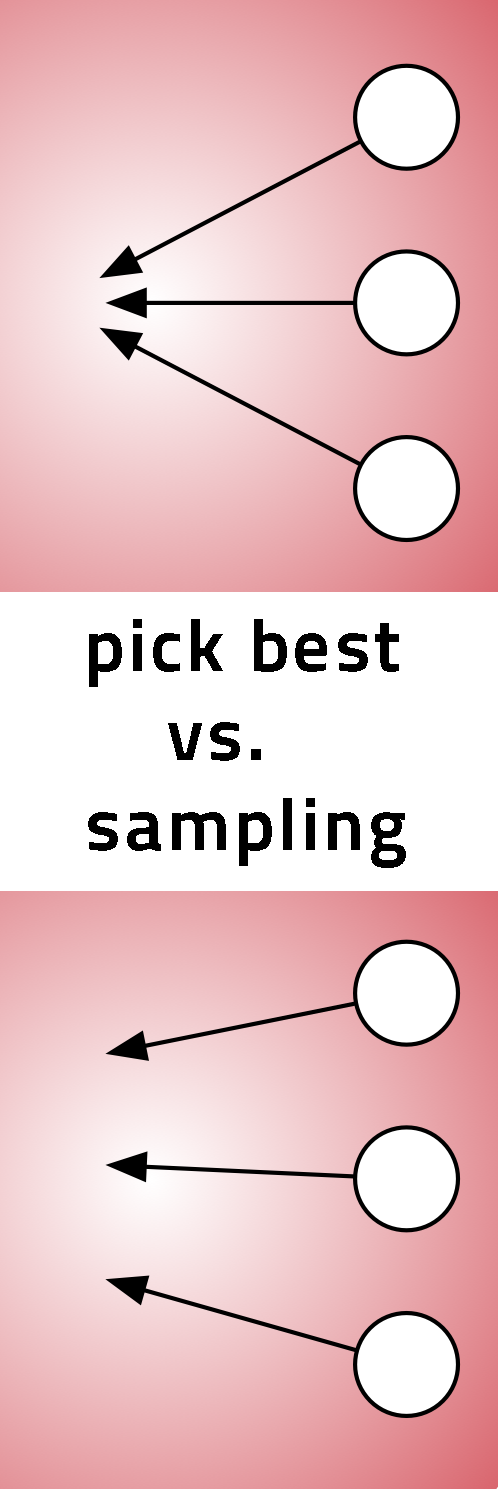
\includegraphics[width=0.16\columnwidth]{images/flee_sample.png}
\caption{Example of $\PP(Dir)$ when fleeing, showing why sampling (BAIS, bottom graphic on the right) may be a better instead of picking the best direction (BAIPB, here $Dir=17$ in the plot, top graphic on the right) and triggering units collisions.}
\label{fig:BayesianUnitChoice}
\end{figure}

We also ran tests in setups with flying units (Zerg Mutalisks) in which BAIPB fared as good as BAIS (no collision for flying units) and way better than OAI.

\subsection{Our bot}

This model is currently at the core of the micro-management of our StarCraft bot. In a competitive micro-management setup, we had a tie with the winner of AIIDE 2010 StarCraft micro-management competition, winning with ranged units (Protoss Dragoons), losing with contact units (Protoss Zealots) and having a perfect tie (the host wins thanks to a few less frames of lag) in the flying units setting (Zerg Mutalisks and Scourges).

This model can be used to specify the behavior of units in RTS games. Instead of relying on a ``units push each other'' physics model for handling dynamic collision of units, this model makes the units react themselves to collision in a more realistic fashion (a marine cannot push a tank, the tank will move). More than adding realism to the game, this is a necessary condition for efficient micro-management in StarCraft: Brood War, as we do not have control over the game physics engine and it does not have this ``flow-like'' physics for units positioning.

\section{Discussion}

\subsection{Perspectives}

\subsubsection{Adding a Sensory Input: Height Attraction}
We make an example of adding a sensory input (that we sometimes use in our bot): height attraction. From a tactical point of view, it is interesting for units to always try to have the higher ground as lower ranged units have a high miss rate (almost 50\%) on higher positioned units. For each of the direction tiles $Dir_i$, we just have to introduce a new set of sensory variables: $H_{i \in \llbracket 0 \dots n \rrbracket} \in \{normal, high, very\_high, unknown\}$ ($unknown$ can be given by the game engine). $\PP(H_i|Dir_i)$ is just an additional factor in the decomposition: $JD \leftarrow JD \times \Pi_{i=1}^{n}\PP(H_i|Dir_i)$. The probability table looks like:
\begin{center}
\begin{tabular}{|l|c|}
\hline
$H_i$ & $dir_i$ \\
\hline
normal & 0.2 \\
high & 0.3 \\
very\_high & 0.45 \\
unknown & 0.05 \\
\hline
\end{tabular}
\end{center}
%%% \begin{center}
%%% \begin{tabular}{|l|c|c|}
%%% \hline
%%% $H_i$ & $dir_i$ & $\bar{dir_i}$ \\
%%% \hline
%%% normal & 0.2 & 0.25 \\
%%% high & 0.3 & 0.25 \\
%%% very\_high & 0.45 & 0.25 \\
%%% unknown & 0.05 & 0.25 \\
%%% \hline
%%% \end{tabular}
%%% \end{center}

\subsubsection{Even More Realistic Behaviors}
The realism of units movements can also be augmented with a simple-to-set $\PP(Dir^{t-1}|Dir^t)$ steering parameter, although we do not use it in the competitive setup. We introduce $Dir_{i \in \llbracket 1 \dots n\rrbracket }^{t-1} \in \{True, False\}$: the previous selected direction, $Dir_i^{t-1} = T$ \textit{iff} the unit went to the direction $i$, else $False$ for a steering (smooth) behavior. The $JD$ would then be $JD \times \Pi_{i=1}^{n} \PP(Dir_i^{t-1} | Dir_i)$, with $\PP(Dir_i^{t-1} | Dir_i)$ the influence of the last direction, either a dot product (with minimal threshold) as before for the objective and flocking, or a parametrized Bell shape over all the $i$.

\subsubsection{Reinforcement Learning}
Future work could consist in using reinforcement learning \citep{Sutton} or evolutionary algorithms \citep{SmithCIG10} to learn the probability tables. It should enhance the performance of our Bayesian units in specific setups. It implies making up challenging scenarii and dealing with huge sampling spaces \citep{Asmuth09}. We learned the distribution of $\PP(Dmg_i | Dir_i)$ through simulated annealing on a specific fight task (by running thousands of games). Instead of having 4 parameters of the probability table to learn, we further restrained $\PP(Dmg_i|Dir_i)$ to be a discrete exponential distribution and we optimized the $\lambda$ parameter. When discretized back to the probability table (for four values of $Dmg$), the parameters that we learned, by optimizing the efficiency of the army in a fixed fight micro-management scenario, were even more risk adverse than the table presented with this model. The major problem with this approach is that parameters which are learned in a given scenario (map, setup) are not trivially re-usable in other setups, so that boundaries have to be found to avoid over-learning/optimization, and/or discovering in which typical scenario our units are at a given time.

\subsubsection{Reducing Collisions}
Also, there are yet many collision cases that remain unsolved (particularly visible with contact units like Zealots and Zerglings), so we could also try adding local priority rules to solve collisions (for instance through an asymmetrical $\PP(Dir_i^{t-1}|Dir_i)$) that would entails units crossing lines with a preferred side (some kind of ``social rule''),
%\item use a units group level supervision using Bayesian units' distributions over $Dir$ as preferences or constraints (for a solver),
%\item use $\PP(Dir)$ as an input to another Bayesian model at the units group level of reasoning.

In collision due to concurrency for ``best'' positions: as seen in Figure.~\ref{fig:BayesianUnitChoice}, units may compete for a well of potential. The solution that we use is to sample in the $Dir$ distribution, which gives better results than picking the most probable direction as soon as there are many units. Another solution, inspired by \citep{Marthi05concurrenthierarchical}, would be for the Bayesian units to communicate their $Dir$ distribution to the units group which would give orders that optimize either the sum of probabilities, or the minimal discrepancy in dissatisfaction, or the survival of costly units (as shown in Fig.~\ref{fig:BayesianUnitsGroup}). Ideally, we could have a full Bayesian model at the \texttt{UnitsGroup} level, which takes the $\PP(Dir)$ distributions as sensory inputs and computes orders to units. This would be a centralized model but in which the complexity of micro-management would have been broken by the lower-level model presented in this chapter.

\begin{figure}[h]
\begin{center}
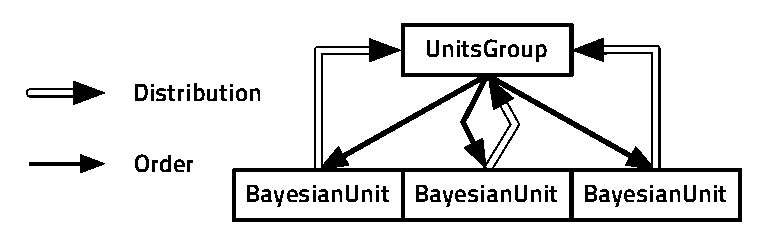
\includegraphics[width=8cm]{images/UnitsGroup_BayesianUnits.pdf}
\caption{Example of the decision taken at the units group level from ``compressed'' information in the form of the distribution on $Dir$ for each Bayesian unit. This can be viewed as a simple optimization problem (maximize sum of probabilities of decisions taken), or as a constraint satisfaction problem (CSP) like ``no unit should be left behind/die/dissatisfied'', or even as another sensory-motor problem with higher-level inputs ($Dir$ distributions). Related to \ref{BayesianUnitCCL}}
\label{fig:BayesianUnitsGroup}
\end{center}
\end{figure}

\subsubsection{Tuning Parameters}
If we learn the parameters of such a model to mimic existing data (data mining) or to maximize a reward function (reinforcement learning), we can interpret the parameters that will be obtained more easily than parameters of an artificial neural network for instance. Parameters learned in one setup can be reused in another if they are understood. We claim that specifying or changing the behavior of this model is much easier than changing the behavior generated by a FSM, and game developers can have a fine control over it. Dynamic switches of behavior (as we do between the scout/flock/inposition/fight modes) are just one probability tables switch away. In fact, probability tables for each sensory input (or group of sensory inputs) can be linked to \textit{sliders} in a \textit{behavior editor} and game makers can specify the behavior of their units by specifying the degree of effect for each perception (sensory input) on the behavior of the unit and see the effect in real time. This is not restricted to RTS and could be applied to \glos{RPG} and even \glos{FPS} \gloss{gameplay}.

\subsubsection{Avoiding Local Optima}
Local optimum could trap and struck our reactive, small look-ahead, units: concave (strong) repulsors (static terrain, very high damage field). A pragmatic solution to that is to remember that the $Obj$ sensory inputs come from the pathfinder and have its influence to grow when in difficult situations (not moved for a long time, concave shape detected...). Another solution is inspired by ants: simply release a repulsive field (a repulsive ``pheromone'') behind the unit and it will be repulsed by places it already visited instead of oscillating around the local optima (see Fig.~\ref{fig:BayesianTrailingPheromone}).

\begin{figure}[h]
\begin{center}
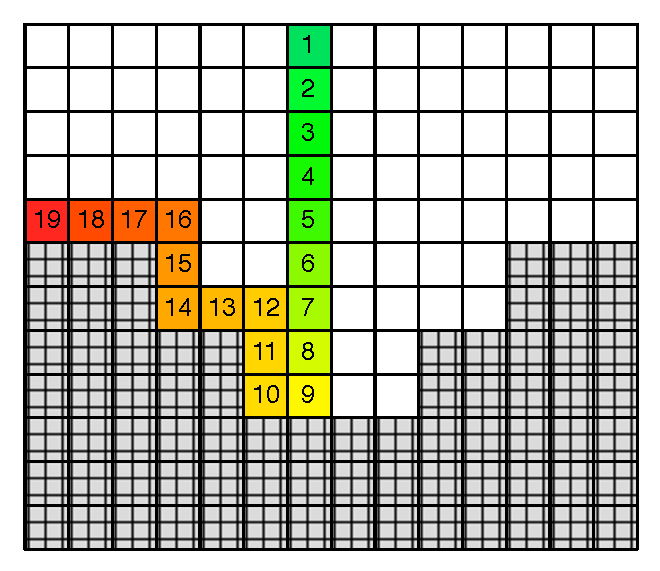
\includegraphics[width=7.4cm]{images/trailing_pheromones.pdf}
\caption{Example of trailing repulsive charges (repulsive ``pheromones'') at already visited positions for Bayesian units to avoid being blocked by local optimums. The trajectory is indicated by the increasing numbers (most recent unit position in 19) and the (decaying) strength of the trailing repulsion is weaker in green and stronger in red. Related to \ref{BayesianUnitCCL}.}
\label{fig:BayesianTrailingPheromone}
\end{center}
\end{figure}

Another solution would be to consider more than just the atomic directions. Indeed, if one decides to cover a lot of space with directions (\textit{i.e.} use this model for with path-planning), one needs to consider directions whose paths collide with each others: if a direction is no longer atomic, this means that there are at least two paths leading to it, from the current unit position. The added complexity of dealing with these paths (and their possible collision routes with allier units or going through potential damages) may not be very aligned with the very reactive behavior that we envisioned here, but an in-between our proposed solution and full path-planning, for which it is costly to consider several dynamic different influences leading to frequent re-computation.

\subsubsection{Probabilistic Modality}
Finally, we could use multi-modality \citep{Colas10} to get rid of the remaining (small: fire-retreat-move) FSM. Instead of being in ``hard'' modes, the unit could be in a weighted sum of modes (summing to one) and we would have:
\ifthenelse{\equal{\myprintformat}{true}}{
\begin{footnotesize}
}{}
$$\PP(Dir) = w_{fightMove()}\PP(Dir|sensory\_inputs)_{fightMove()} + w_{flee()}\PP(Dir|sensory\_inputs)_{flee()} \dots$$
\ifthenelse{\equal{\myprintformat}{true}}{
\end{footnotesize}
}{}
This could particularly help dealing with the fact that parameters learned from fixed scenarii would be too specialized. This way we could interpolate a continuous family of distributions for $\PP(Dir)$ from a fixed and finite number of parameters learned from a finite number of experiments setups.

%The sensory inputs given to a ``Bayesian unit'' controls its objective(s) or goal(s) and the parametrization of his probabilistic model controls its behavior and degree of freedom. As an illustration, two of the extreme cases are $\PP(Direction=x|Objective=x)=1$: no freedom, $\PP(Direction=x|Objective=y)=\PP(Direction=x)$: no influence of the objective. %%% TODO

\subsection{Conclusion}
\label{BayesianUnitCCL}
We have implemented this model in StarCraft, and it outperforms the original AI as well as other bots. Our approach does not require a specific vertical integration for each different type of objectives (higher level goals), as opposed to CBR and reactive planning \citep{Ontanon2007,WeberCIG10}: it can have a completely different model above feeding sensory inputs like $Obj_i$. It runs in real-time on a laptop (Core 2 Duo) taking decisions for every units 24 times per second. It scales well with the number of units to control thanks to the absence of communication at the unit level, and is more robust and maintainable than a FSM. Particularly, the cost to add a new sensory input (a new effect on the units behavior) is low.


\chapter{Tactics}
\begin{figure}[!ht]
\begin{center}
\includegraphics[width=13cm]{images/starcraft_bbq_concept_TACTICS.pdf}
\end{center}
\label{fig:conceptTACTICS}
\caption{Information-centric view of the architecture of the bot, the part concerning this chapter is in the dotted rectangle}
\end{figure}
\begin{itemize}
\item Problem: choose which tactical actions/goals to persue, peform the action
\item Complexity: incompleteness/uncertainty problem, lot of low level information to handle, w.r.t. full and higher level information, simple.
\item State of the art: \citep{SORTS, Weber2010cr, UCT, CadenaG11}
\item Our take: low level heuristics that we learn to adapt to
\item Results: XXX
\item Conclusion and perspectives: still enabled for meta-game, and even in-game, adaptation. Could learn the action sequences of tactics from replays ($\approxeq$HMM).
\end{itemize}

\section{What are Tactics?}
\section{Related Works}
\section{A Bayesian Tactical Model}
\section{Results on StarCraft}
\section{Extensions}



\chapter{Strategy}
\label{chapter:strategy}
\begin{quotation}
\textit{Strategy without tactics is the slowest route to victory. Tactics without strategy is the noise before defeat.}\\
%%% \begin{flushright}Sun Tzu (The Art of War, 476-221 BC)\end{flushright}
\textit{All men can see these tactics whereby I conquer, but what none can see is the strategy out of which victory is evolved.}\\
\begin{flushright}Sun Tzu (The Art of War, 476-221 BC)\end{flushright}
\end{quotation}

\lettrine{W}e present our solutions to some of the dimensions of strategies. The main idea is to reduce the complexity encoding all possible variations of strategies to a few strong indicators: the \glos{buildtree} (closely related to the \glos{techtree}) and canonical army compositions. We also try and abstract early game strategies to ``openings'' (as in Chess). Build trees estimation was published at the Annual Conference on Artificial Intelligence and Interactive Digital Entertainment (AAAI AIIDE) 2011 in Palo Alto \citep{SYNNAEVE:StratPred} and openings prediction was published at Computational Intelligence in Games (IEEE CIG) 2011 in Seoul \citep{SYNNAEVE:OpeningPred}.

\ifthenelse{\equal{\myebookformat}{false}}{
\chaptertoc
}{}

\newglossaryentry{EM}{name=EM,description={expectation-maximization, an iterative method to optimize parameters of statistical models depending on unobserved variables. The expectation (E) step gives the likelihood depending on the latent variables, and the maximization (M) step computes maximizing parameters for the expectation of this likelihood.}}

\newglossaryentry{BIC}{name=BIC,description={Bayesian information criterion, a score for model selection. For a given model with $n$ data points, $k$ parameters and $L$ the maximum likelihood, $BIC= -2 \ln(L) + k \ln(n)$}}

\newglossaryentry{GMM}{name=GMM,description={Gaussian mixture model, a generative model in which observations are the outcomes of mixtures of normal distribution.}}

\begin{figure}[!ht]
\begin{center}
\includegraphics[width=0.84\columnwidth]{images/starcraft_bbq_concept_STRATEGY.pdf}
\end{center}
\caption{Information-centric view of the architecture of the bot, the part concerning this chapter is in the dotted rectangle}
\label{fig:conceptSTRATEGY}
\end{figure}

\begin{itemize}
\item Problem: take the winning strategy in the absolute (knowing everything: complete observations, players intentions, effects of each possible actions).
\item Problem that we solve: take the winning strategy (in average) knowing what we saw from the opponent and our model of the game. 
\item Type: prediction is problem of \textit{inference} or \textit{plan recognition} from \textit{incomplete informations}; adaptation given what we know is a problem of \textit{planning under constraints}.
\item Complexity: simple StarCraft decision problems are \textsc{np}-hard \citep{GamingComplexity}, basic StarCraft strategy with full information (remember that StarCraft is partially observable) is mappable to the Generalized Geography problem and thus is \textsc{pspace}-hard \citep{Lichtenstein78}, Chess \citep{Fraenkel81} and Go (with Japanese ko rules) are \textsc{exptime}-complete \citep{Robson83}. Our solutions are real-time on a laptop. %%% TODO XXX
%\item Results: better resistance to noise, which is fundamental in real setup RTS gameplay (fog of war). Full Bayesian model down to adaptation actions some day?
%\item Conclusion and perspectives: a way to encode and use gameplay/structural knowledge 
\end{itemize}

\section{What is a Strategy?}
% tech tree, opening, army composition, build tree

%In a RTS, players need to gather resources to build military units and defeat their opponents. To that end, they often have \textit{worker units} (or extraction structures) than can gather resources needed to build \textit{workers}, \textit{buildings}, \textit{military units} and \textit{research upgrades}. Workers are often also builders (as in StarCraft) and are weak in fights compared to military units. Resources may have different uses, for instance in StarCraft: minerals are used for everything, whereas gas is only required for advanced buildings or military units, and technology upgrades. Buildings and research upgrades define technology trees (directed acyclic graphs) and each state of a ``tech tree'' allow for different unit type production abilities and unit spells/abilities. The military can be of different types, any combinations of ranged, casters, contact attack, zone attacks, big, small, slow, fast, invisible, flying... Units can have attacks and defenses that counter each others as in rock-paper-scissors. We consider \textit{strategy} the way to expand the tech tree as well as the army composition, because both require long term planning under uncertainty, and a risk-reward trade-off. 

As it is an abstract concept, what constitutes \textit{strategy} is hard to grasp. The definition that we use for strategy is a combination of aggressiveness and ``where do we put the cursor/pointer/slider between economy, technology and military production?''. It is very much related to where we put our resources:
\begin{itemize}
    \item If we prioritize economy, on a short term basis our army strength (numbers) may suffer, but on the longer term we will be able to produce more, or produce equally and still expand our economy or technology in parallel. Also, keep in mind that resources depletes mineral deposits/gas geysers can be exhausted/drained.
    \item If we prioritize technology, on a short term basis our army strength may suffer, on the longer term it can strive with powerful units or units which are adapted to the enemy's.
    \item If we prioritize military production, on a short term basis our army strength will strive, but we will not be able to adapt our army composition to new unit types nor increase our production throughput.
\end{itemize}
Strategy is a question of balance between these three axis, and of knowing when we can attack and when we should stay in defense. Being aggressive is best when we have a military advantage (in numbers or technology) over the opponent. Advantages are gained by investments in these axis and using them when we max out our returns (comparatively to the opponent's).

The challenges for an AI enabled/empower with strategic reasoning is to be able to assess the strategic situation of the game (both for itself and for the opponent) and to position these two pointers as best as it can.

\section{Related Work}

%This work was encouraged by the reading of Weber and Mateas' Data Mining Approach to Strategy Prediction \citep{weberStrat} and the fact that they provided their dataset, that we used. They tried and evaluated several machine learning algorithms on replays that were labeled with strategies (openings) with rules.

There are precedent works of Bayesian plan recognition \citep{BMPR}, even in games with \citep{BayesianRecog} using dynamic Bayesian networks to recognize a user's plan in a multi-player dungeon adventure. Commercial RTS games most commonly use \glos{FSM} \citep{FSM_AIGameProgWisdom2003} to encode strategies and their transitions.

There are related works in the domains of opponent modeling \citep{HsiehS08,schadd2007opponent,Kabanza2010}. The main methods used to these ends are case-based reasoning (CBR) and planning or plan recognition \citep{LTW,CBR_Planning,OntanonCBR,HTNPlanning,Ramirez}.

\cite{LTW} used CBR to perform dynamic plan retrieval extracted from domain knowledge in Wargus (Warcraft II open source clone). \cite{CBR_Planning} base their real-time case-based planning (CBP) system on a plan dependency graph which is learned from human demonstration in Wargus. In \citep{OntanonCBR,PlanRetrieval}, they use CBR and expert demonstrations on Wargus. %They update their previous CPB approach by using ``situation assessment'' for plan retrieval. 
They improve the speed of CPB by using a decision tree to select relevant features. \cite{HsiehS08} based their work on \citep{LTW} and used StarCraft replays to construct states and building sequences. Strategies are choices of building construction order in their model. 

\cite{schadd2007opponent} describe opponent modeling through hierarchically structured models of the opponent behaviour and they applied their work to the Spring RTS (Total Annihilation open source clone). \cite{HTNPlanning} use hierarchical task networks (\glos{HTN}) to model strategies in a first person shooter with the goal to use HTN planners. \cite{Kabanza2010} improve the probabilistic hostile agent task tracker (PHATT \citep{PHATT}, a simulated \glos{HMM} for plan recognition) by encoding strategies as HTN. 

\cite{weberStrat} presented ``a data mining approach to strategy prediction'' and performed supervised learning (from buildings features) on labeled StarCraft replays. In this chapter, for openings prediction, we worked with the same dataset as they did, using their openings labels and comparing it to our own labeling method. %\cite{Weber2010qf} applied this automated replay annotation approach to CBP on StarCraft.

\cite{HMMstrat_RTS_AIIDE11} presented their work at the same conference that we presented \citep{SYNNAEVE:StratPred}. They used an HMM which states are extracted from (unsupervised) maximum likelihood on the dataset. The HMM parameters are learned from unit counts (both buildings and military units) every 30 seconds and Viterbi inference is used to predict the most likely next states from partial observations. 


\section{Perception and Interaction}

\subsection{Buildings}
\label{sec:buildings}

From last chapter (section~\ref{sec:techtree}), we recall the \textit{\glos{techtree}} is a directed acyclic graph which contains the whole technological (buildings and upgrades) development of a player. Also, each unit and building has a \textit{sight range} that provides the player with a view of the map. Parts of the map not in the sight range of the player's units are under \textit{fog of war} and the player ignores what is and happens there. 

%%% BUILD TREES vs TECH TREES TODO
\glos{buildorder}

\subsection{Openings}
\label{sec:openings}

In RTS games jargon, an \textit{\glos{opening}} denotes the same thing than in Chess: an early game plan for which the player has to make choices. In Chess because one can not move many pieces at once (each turn), in RTS games because during the development phase, one is economically limited and has to choose between economic and military priorities and can only open so many tech paths at once. The \glos{opening} corresponds to the first military (tactical) moves that will be performed and, in StarCraft, it corresponds to the 5 (early rushes) to 15 minutes (advanced technology / late push) timespan. 

Players have to find out what opening their opponents are doing to be able to effectively deal with the strategy (army composition) and tactics (military moves: where and when) thrown at them. For that, players scout each other and reason about the incomplete information they can bring together about army and buildings composition. This chapter presents a probabilistic model able to predict the \textit{\glos{opening}} of the enemy that is used in a StarCraft AI competition entry bot. Instead of hard-coding strategies or even considering plans as a whole, we consider the long term evolution of our \glos{techtree} and the evolution of our army composition separately (but steering and constraining each others), as shown in Fig.~\ref{bbq_dataflow}. With this model, our bot asks ``what units should I produce?'' (assessing the whole situation), being able to revise and adapt its production plans.

Later in the game, as the possibilities of strategies ``diverge'' (as in Chess), there are no longer fixed foundations/terms that we can speak of as for openings. Instead, what is interesting is to know the technologies available to the enemy as well as have a sense of the composition of their army. The players have to adapt to each other technologies and armies compositions either to be able to defend or to attack. Some units are more cost-efficient than others against particular compositions. Some combinations of units play well with each others (for instance biological units with ``medics'' or a good ratio of strong contact units backed with fragile ranged or artillery units). Finally, some units can be game changing by themselves like cloaking units, detectors, massive area of effects units... 

\subsection{Military Units}
\label{sec:militaryunits}


\section{Replays Labeling}

\subsection{Dataset}

We used Weber and Mateas \citep{weberStrat} dataset of labeled replays. It is composed of 8806 StarCraft: Broodwar game logs, the details are given in Table~\ref{tab:datasetweber}. A \glos{matchup} is a set of the two opponents races: Protoss versus Terran (PvT) is a match-up, Protoss versus Zerg (PvZ) is another one. They are distinguished because strategies distribution are very different across match-ups (see Tables~\ref{tab:datasetweber} and \ref{openings_distrib}). Weber and Mateas used logic rules on building sequences to put their labels, concerning only tier 2 strategies (no tier 1 rushes).

\begin{table}[!h]
\begin{center}
\begin{footnotesize}
\begin{tabular}{|l|c|c|c|l|c|c|c|l|c|c|c|}
\hline
opening & PvP & PvT & PvZ & opening & TvP & TvT & TvZ & opening & ZvP & ZvT & ZvZ \\
\hline
FastLegs & 4 & 17 & 108 & Bio & 144 & 41 & 911 & Lurker & 33 & 184 & 1 \\
FastExpand & 119 & 350 & 465 & Unknown & 66 & 33 & 119 & Unknown & 159 & 164 & 212 \\
ReaverDrop & 51 & 135 & 31 & Standard & 226 & 1 & 9 & HydraRush & 48 & 13 & 9 \\
FastObs & 145 & 360 & 9 & SiegeExpand & 255 & 49 & 7 & Standard & 40 & 80 & 1 \\
Unknown & 121 & 87 & 124 & VultureHarass & 134 & 226 & 5 & TwoHatchMuta & 76 & 191 & 738 \\
Carrier & 2 & 8 & 204 & TwoFactory & 218 & 188 & 24 &  HydraMass & 528 & 204 & 14 \\
FastDT & 100 & 182 & 83 & FastDropship & 96 & 90 & 75 & ThreeHatchMuta & 140 & 314 & 35 \\
\hline
total & 542 & 1139 & 1024 & total & 1139 & 628 & 1150 & total & 1024 & 1150 & 1010 \\
\hline
\end{tabular}
\end{footnotesize}
\end{center}
\caption{Weber's dataset with its labels. XvY means the XvY or YvX match-up but the openings numbers are presented for X.}
\label{fig:weberdatasetnumbers}
\end{table}

\subsection{Our Labeling}

\subsubsection{The Pitfall of Logical/Rule-based Labeling}
Openings are closely related to \gloss{buildorder} (BO) but different BO can lead to the same opening and some BO are shared by different openings. Particularly, if we do not take into account the time at which the buildings are constructed, we may have a wrong opening label too often: if an opening consist in having building C as soon as possible, it does not matter if we built B-A-C instead of the standard A-B-C as long as we have built C quickly. That is the kind of case that will be overlooked by logical labeling. For that reason, we tried to label replays with the statistical appearance of key features with a semi-supervised method (see Figure~\ref{replays_labeling}). Indeed, the purpose of our opening prediction model is to help our StarCraft playing bot to deal with rushes and special tactics. This was not the main focus of Weber and Mateas' labels, which follow exactly the build tree. So, we used the key components of openings that we want to be aware of as features for our labeling algorithm as shown in Table~\ref{labels}.

\begin{figure}[h]
\centerline{\includegraphics[width=0.80\columnwidth]{images/replays_labeling.pdf}}
\caption{Data centric view of our semi-supervised labeling of replays}
\label{replays_labeling}
\end{figure}

\subsubsection{Features}

The selection of the features along with the opening labels is the supervised part of our labeling method. The knowledge of the features and openings comes from expert play and the StarCraft Liquipedia\footnote{\url{http://wiki.teamliquid.net/starcraft/}} (a Wikipedia for StarCraft). They are all presented in Table~\ref{labels}. For instance, if we want to find out which replays correspond to the ``fast Dark Templar'' (DT, Protoss invisible unit) opening, we put the time at which the first Dark Templar is constructed as a feature and perform clustering on replays with it. This is what is needed for our playing bot: to be able to know when he has to fear ``fast DT'' opening and build a detector unit quickly to be able to deal with invisibility.

\begin{table}[h] \caption{Opening/Strategies labels of the replays (Weber's and ours are not always corresponding)}
\begin{footnotesize}
\begin{center}
\begin{tabular}{|c|c|ccc|}
\hline
Race
& Weber's labels
& Our labels
& Features 
& Note (what we fear) \\ \hline
Protoss & FastLegs & speedzeal & Legs, GroundWeapons+1 & quick speed+upgrade attack\\
 & FastDT & fast\_dt & DarkTemplar & invisible units\\
 & FastObs & nony & Goon, Range & quick long ranged attack\\
 & ReaverDrop & reaver\_drop & Reaver, Shuttle & tactical attack zone damages \\
 & Carrier & corsair & Corsair & flying units \\
 & FastExpand & templar & Storm, Templar & powerful zone attack \\
 &  & two\_gates & 2ndGateway, Gateway, Zealot & aggressive rush \\
 & Unknown & unknown & (no clear label) & \\ \hline
Terran  & Bio & bio & 3rdBarracks, 2ndBarracks, Barracks & aggressive rush\\ 
 & TwoFactory & two\_facto & 2ndFactory & strong push (long range) \\ 
 & VultureHarass & vultures & Mines, Vulture & aggressive harass, invisible\\ 
 & SiegeExpand & fast\_exp & Expansion, Barracks & economical advantage \\ 
 & Standard & & & \\ 
 & FastDropship & drop & DropShip & tactical attack \\ 
 & Unknown & unknown & (no clear label) & \\ \hline
Zerg & TwoHatchMuta & fast\_mutas & Mutalisk, Gas & early air raid \\
 & ThreeHatchMuta & mutas & 3rdHatch, Mutalisk & massive air raid \\
 & HydraRush & hydras & Hydra, HydraSpeed, HydraRange & quick ranged attack\\
 & Standard & (speedlings) & (ZerglingSpeed, Zergling) & (removed, quick attacks/mobility) \\
 & HydraMass & & & \\
 & Lurker & lurkers & Lurker & invisible and zone damages \\
 & Unknown & unknown & (no clear label) & \\ \hline
\end{tabular}
\label{labels}
\end{center}
\end{footnotesize}
\end{table}

\begin{table}[h]
\caption{Openings distributions for Terran in all the match-ups}
\begin{center}
\begin{tabular}{|c|cc|cc|cc|}
\hline
&  & vs Protoss &  & vs Terran &  & vs Zerg \\
Opening
& Nb
& \begin{scriptsize}Percentage\end{scriptsize}
& Nb
& \begin{scriptsize}Percentage\end{scriptsize}
& Nb
& \begin{scriptsize}Percentage\end{scriptsize} \\ \hline
%%%two\_gates & 332 & & 252 & & 304 & \\
%%%fast\_dt & 7 & & 87 & & 20 & \\
%%%templar & 3 & & 17 & & 22 & \\
% TvP 1007
% TvT 576
% TvZ 872
bio 	    & 62 	& 6.2 	& 25 	& 4.4   & 197 	& 22.6 \\
fast\_exp 	& 438 	& 43.5 	& 377 	& 65.4  & 392 	& 44.9 \\
two\_facto 	& 240 	& 23.8  & 127 	& 22.0  & 116 	& 13.3 \\
vultures 	& 122 	& 12.1  & 3 	& 0.6   & 3 	& 0.3  \\
drop 	    & 52 	& 5.2   & 10 	& 1.7   & 121 	& 13.9 \\
unknown 	& 93 	& 9.3   & 34 	& 5.9   & 43 	& 5.0 \\ \hline
\end{tabular}
\label{openings_distrib}
\end{center}
\end{table}

\subsubsection{Clustering}

For the clustering part, we tried k-means and expectation-maximization (\glos{EM}, with Gaussian mixtures) on Gaussian mixtures with shapes and volumes chosen with a Bayesian information criterion (\glos{BIC}). Best BIC models were almost always the most agreeing with expert knowledge (15/17 labels), so we kept this method. We used the R package Mclust \citep{Mclust,Mclust2} to perform full EM clustering. 

\label{GMMEM}
The Gaussian mixture model (\glos{GMM}) is as follows:
\begin{itemize}
    \item Variables:
    \begin{itemize}
        \item $X_{i \in \llbracket 1 \dots n\rrbracket}$ the features for the $i$th replay/game. For instance for the ``rax\_fe'' opening (Barracks and fast expand), we used the features ``time of the first expansion'' and ``time of the first Barracks'', as is shown in Figure~\ref{TvZraxFE}, and each data point is an $X_i$.
        \item $Op_{i \in \llbracket1 \dots n\rrbracket}$ the opening of game $i$. Instead of doing one clustering with $k$ possible openings, we did $k$ clusterings of 1 opening vs the rest. So for us $Op_i \in \{opening, rest\}$.
    \end{itemize}
    \item Decomposition:
$$\PP(X_{1:n}, Op_{1:n}) = \prod_{i=1}^n \PP(X_i|Op_i)\PP(Op_i)$$
    \item Forms, for the $k$ openings we have, with $f$ features:
    \begin{itemize}
        \item $\PP(X_i|Op_i) = \sum_{j \in \{op,\neg op\}} \mathcal{N}(\mu_j, \sigma_j^2)$ 
        \item $\PP(Op_i) = Bernouilli(p_{op})$: $\PP(Op_i=op) = p_{op}, \PP(Op_i=\neg op) = 1-p_{op}$
    \end{itemize}
    \item Identification (EM with maximum likelihood\footnote{Maximum a posteriori (MAP) would maximize the joint.}):\\
    Let $\theta= (\mu_{1:2k},\sigma_{1:2k})$, initialize $\theta$ randomly, and let\\
 $L(\theta;X) = \PP(X|\theta) = \prod_{i=1}^n \sum_{Op}\PP(X|\theta,Op)\PP(Op)$, iterate until convergence:
    \begin{enumerate}
        \item E-step: $Q(\theta|\theta^{(t)})= \mathrm{E}[\log L(\theta;x,Op)] = \mathrm{E}[\log \prod_{i=1}^n \sum_{Op_i}\PP(x_i|Op_i,\theta)\PP(Op_i)]$
        \item M-step: $\theta^{(t+1)}=\argmax_{\theta} Q(\theta|\theta^{(t)})$
    \end{enumerate}

    \item Question:
$$\PP(Op_{1:n} | X_{1:n}) \propto \PP(X_{1:n}|Op_{1:n})\PP(Op_{1:n})$$
\end{itemize}
The $\sigma_j$ matrices can define Gaussian distribution of any combinations between:
\begin{itemize}
    \item volume (of the normal distributions of each mixtures at a given $\sigma$ value): equal or variable,
    \item shape (of the multidimensional normal distributions of each mixtures): equal or variable, 
    \item orientation: spherical (i.e. no orientation), coordinate axes, equal (any orientation although the same for all mixtures components) or variable (any orientation for any component).
\end{itemize}
We chose the combinations with the best (i.e. smallest) \glos{BIC} score. For a given model with $n$ data points, $m$ parameters and $L$ the maximum likelihood, $BIC= -2 \ln(L) + m \ln(n)$. A $\sigma$ with variable volume, variable shape and variable orientation is also called a full covariance matrix.

\begin{figure}[hp]
\centerline{\includegraphics[width=0.56\columnwidth]{images/PvTfastDT.png}}
\caption{Protoss vs Terran distribution of first appearance of Dark Templars (Protoss invisible unit).}
\label{PvTfastDT}
\end{figure}

\begin{figure}[hp]
\centerline{\includegraphics[width=0.7\columnwidth]{images/TvZraxFE.png}}
\caption{Terran vs Zerg Barracks and first Expansion timings (Terran). The bottom left cluster (squares) is the one labeled as \textit{fast\_exp}.}
\label{TvZraxFE}
\end{figure}

\begin{figure}[hp]
\centerline{\includegraphics[width=0.7\columnwidth]{images/PvPspeedzeal.png}}
\caption{Protoss vs Protoss Ground Attack +1 and Zealot Legs upgrades timings. The bottom left cluster (squares) is the one labeled as \textit{speedzeal}.}
\label{PvPspeedzeal}
\end{figure}

\begin{figure}[hp]
\centerline{\includegraphics[width=0.7\columnwidth]{images/ZvPmutas.png}}
\caption{Zerg vs Protoss time of the third Hatch and first appearance of Mutalisks. The bottom left cluster (squares) is the one labeled as \textit{mutas}.}
\label{ZvPmutas}
\end{figure}

\subsubsection{Labeling, Score Filtering}

We produce ``2 bins clustering'' for each set of features (corresponding to each opening), and label the replays belonging to the cluster with the lower norm of features' appearances (that is exactly the purpose of our features). Figures~\ref{PvPspeedzeal}, \ref{TvZraxFE}
and \ref{ZvPmutas} show the clusters out of EM with the features of the corresponding openings. We thought of clustering because there are two cases in which you build a specific military unit of research a specific upgrade: either it is part of your opening, or it is part of your longer term game plan or even in reaction to the opponent. So the distribution over the time at which a feature appears is bimodal, with one (sharp) mode corresponding to ``opening with it'' and the other for the rest of the games, as can be seen in Figure~\ref{PvTfastDT}.

Finally, some replays are labeled two or three times with different labels (due to the different time of effect of different openings), so we apply a score filtering to transform multiple label replays into unique label ones (see Figure~\ref{replays_labeling}). For that we choose the openings labels that were happening the earliest (as they are a closer threat to the bot in a game setup) if and only if they were also the most probable or at 10\% of probability of the most probable label (to exclude transition boundaries of clusters) for this replay. We find the earliest by comparing the norms of the clusters means in competition. All replays without a label or with multiple labels (\textit{i.e.} which did not had a unique solution in filtering) after the filtering were labeled as \textit{unknown}. We then used this labeled dataset as well as Weber and Mateas' labels in the testing of our Bayesian model for opening prediction.


\section{Build Tree Prediction}
\label{sec:strategyprediction}
The work described in this section can be classified as probabilistic plan recognition. Strictly speaking, we present model-based machine learning used for prediction of plans, while our model is not limited to prediction. We performed two levels of plan recognition, both are learned from the replays: tech tree prediction (unsupervised, this section) and opening prediction (semi-supervised or supervised depending on the labeling method, next section).

\begin{quotation}\textit{
What is of supreme importance in war is to attack the enemy's strategy.}\\
Sun Tzu\end{quotation}

\label{sec:techtreepred}
%\subsubsection{Variables}
%\subsubsection{Decomposition}
%\subsubsection{Forms}
%\subsubsection{Identification (learning)}
%\subsubsection{Questions}

\subsection{Results on StarCraft}


\subsubsection{Prediction}

For each match-up, we ran cross-validation testing with 9/10th of the dataset used for learning and the remaining 1/10th of the dataset used for testing. We ran tests finishing at 5, 10 and 15 minutes to capture all kinds of openings (early to late ones). To measure the predictive capability of our model, we used 3 metrics: 
\begin{itemize}
\item the \textit{final} prediction, which is the opening that is predicted at the end of the test, 
\item the \textit{online twice} (OT), which counts the openings that have emerged as most probable twice a test (so that their predominance is not due to noise),
\item the \textit{online once} $> 3$ (OO3), which counts the openings that have emerged as most probable openings after 3 minutes (so that these predictions are based on really meaningful information).
\end{itemize}
After 3 minutes, a Terran player will have or be building his first supply depot, barracks, refinery (gas), and at least factory or expansion. A Zerg player would have his first overlord, zergling pool, extractor (gas) and most of the time his expansion and lair tech. A Protoss player would have his first pylon, gateway, assimilator (gas), cybernectics core, and sometimes his robotics center, or forge and expansion.

\begin{figure}[htp]
\centerline{\includegraphics[width=0.8\columnwidth]{images/TvP_prediction.png}}
\centerline{\includegraphics[width=0.8\columnwidth]{images/TvPx_prediction.png}}
\caption{Evolution of $\PP(Opening)$ with increasing observations in a TvP match-up, with Weber's labeling on top, our labeling on the bottom. The x-axis corresponds to the construction of buildings.}
\label{prediction}
\end{figure}

Table~\ref{results} sums up all the prediction probabilities (scores) of our model in all the match-ups with both labeling of the game logs. Please note that when an opening is mispredicted, the distribution on openings is often not $\PP(badopening)=1, \PP(others)=0$ and that we can extract some value out of these distributions. Also, we observed that $\PP(Opening=unknown)>\PP(others)$ is often a case of misprediction: our bot would use the next prediction in this case. Figure~\ref{prediction} shows the evolution of the distribution $\PP(Opening)$ during a replay for Weber's and our labelings. Figure~\ref{noise} shows the resistance of our model to noise. We randomly removed some observations (buildings, attributes), from 1 to 15, knowing that for Protoss and Terran we use 16 buildings observations and 17 for Zerg. We think that our model copes well with noise because it backtracks unseen observations: for instance if we have only the $core$ observation, it will work with build trees containing $core$ that will passively infer unseen $pylon$ and $gate$. Also, uncertainty is handled natively.



\begin{figure}[htp]
\centerline{\includegraphics[width=0.7\columnwidth]{images/ZvP2.png}}
\centerline{\includegraphics[width=0.7\columnwidth]{images/PvZ2.png}}
\caption{Two extreme evolutions of the 3 probabilities of opening recognition with increasing noise (15 missing attributes/observations/buildings correspond to 93.75\% missing information for Protoss and Terran openings prediction and 88.23\% of missing attributes for Zerg openings prediction). Zerg opening prediction probabilitly on top, Protoss bottom.}
\label{noise}
\end{figure}

\begin{sidewaystable}[ht] \caption{Prediction probabilities for all the match-ups}
\begin{center}
\begin{tabular}{|c|ccc|ccc|ccc|ccc|ccc|ccc|}
\hline
& \multicolumn{9}{|c|}{Weber and Mateas' labels}
& \multicolumn{9}{|c|}{Our labels}
\\  \hline
& \multicolumn{3}{|c|}{5 minutes}
& \multicolumn{3}{|c|}{10 minutes}
& \multicolumn{3}{|c|}{15 minutes}
& \multicolumn{3}{|c|}{5 minutes}
& \multicolumn{3}{|c|}{10 minutes}
& \multicolumn{3}{|c|}{15 minutes}
\\
\begin{scriptsize}match-up\end{scriptsize}
& final
& OT
& OO3
& final
& OT
& OO3
& final
& OT
& OO3
& final
& OT
& OO3
& final
& OT
& OO3
& final
& OT
& OO3 \\ \hline
PvP & 0.65 & 0.53 & 0.59 & 0.69 & 0.69 & 0.71 & 0.65 & 0.67 & 0.73
& 0.78 & 0.74 & 0.68 & 0.83 & 0.83 & 0.83 & 0.85 & 0.83 & 0.83 \\
PvT & 0.75 & 0.64 & 0.71 & 0.78 & 0.86 & 0.83 & 0.81 & 0.88 & 0.84
& 0.62 & 0.69 & 0.69 & 0.62 & 0.73 & 0.72 & 0.6 & 0.79 & 0.76 \\
PvZ & 0.73 & 0.71 & 0.66 & 0.8 & 0.86 & 0.8 & 0.82 & 0.87 & 0.8
& 0.61 & 0.6 & 0.62 & 0.66 & 0.66 & 0.69 & 0.61 & 0.62 & 0.62 \\
TvP & 0.69 & 0.63 & 0.76 & 0.6 & 0.75 & 0.77 & 0.55 & 0.73 & 0.75
& 0.50 & 0.47 & 0.54 & 0.5 & 0.6 & 0.69 & 0.42 & 0.62 & 0.65 \\
TvT & 0.57 & 0.55 & 0.65 & 0.5 & 0.55 & 0.62 & 0.4 & 0.52 & 0.58
& 0.72 & 0.75 & 0.77 & 0.68 & 0.89 & 0.84 & 0.7 & 0.88 & 0.8 \\
TvZ & 0.84 & 0.82 & 0.81 & 0.88 & 0.91 & 0.93 & 0.89 & 0.91 & 0.93
& 0.71 & 0.78 & 0.77 & 0.72 & 0.88 & 0.86 & 0.68 & 0.82 & 0.81 \\
ZvP & 0.63 & 0.59 & 0.64 & 0.87 & 0.82 & 0.89 & 0.85 & 0.83 & 0.87
& 0.39 & 0.56 & 0.52 & 0.35 & 0.6 & 0.57 & 0.41 & 0.61 & 0.62 \\
ZvT & 0.59 & 0.51 & 0.59 & 0.68 & 0.69 & 0.72 & 0.57 & 0.68 & 0.7
& 0.54 & 0.63 & 0.61 & 0.52 & 0.67 & 0.62 & 0.55 & 0.73 & 0.66 \\
ZvZ & 0.69 & 0.64 & 0.67 & 0.73 & 0.74 & 0.77 & 0.7 & 0.73 & 0.73
& 0.83 & 0.85 & 0.85 & 0.81 & 0.89 & 0.94 & 0.81 &  0.88 & 0.94\\ \hline
\begin{scriptsize}overall\end{scriptsize} & 0.68 & 0.62 & 0.68 & 0.73 & 0.76 & 0.78 & 0.69 & 0.76 & 0.77 
& 0.63 & 0.67 & 0.67 & 0.63 & 0.75 & 0.75 & 0.63 & 0.75 & 0.74 \\ \hline
\end{tabular}
\label{results}
\end{center}
\end{sidewaystable}


\subsubsection{Performances}
The first iteration of this model was not making use of the structure imposed by the game in the form of ``possible build trees'' and was at best very slow, at worst intractable without sampling. With the model presented here, the performances are ready for production as shown in Table~\ref{CPU}. The memory footprint is around 3.5Mb on a 64bits machine. Learning computation time is linear in the number of games logs events ($O(N)$ with $N$ observations), which are bounded, so it is linear in the number of game logs. It can be serialized and done only once when the dataset changes. The prediction computation corresponds to the sum in the question (III.B.5) and so its computational complexity is in $O(N\cdot M)$ with $N$ build trees and $M$ possible observations, as $M << N$, we can consider it linear in the number of build trees (values of $BuildTree$).

\begin{table}[h]
\caption{Extremes of computation time values (in seconds, Core 2 Duo 2.8Ghz)}
\begin{center}
\begin{tabular}{|c|cc|cc|}
\hline
Race
& Nb Games
& Learning time
& Inference $\mu$
& Inference $\sigma^2$ \\ \hline
T (max) & 1036 & 0.197844 & 0.0360234 & 0.00892601 \\
T \begin{tiny}(Terran)\end{tiny} & 567 & 0.110019 & 0.030129 & 0.00738386 \\ 
P \begin{tiny}(Protoss)\end{tiny} & 1021 & 0.13513 & 0.0164457 & 0.00370478 \\
P \begin{tiny}(Protoss)\end{tiny} & 542 & 0.056275 & 0.00940027 & 0.00188217 \\ 
Z \begin{tiny}(Zerg)\end{tiny} & 1028 & 0.143851 & 0.0150968 & 0.00334057 \\
Z \begin{tiny}(Zerg)\end{tiny} & 896 & 0.089014 & 0.00796715 & 0.00123551 \\ \hline
\end{tabular}
\label{CPU}
\end{center}
\end{table}



\section{Early Game: Openings}

\subsection{Opening Prediction Model}
We now build up on buildings prediction to make opening prediction % TODO

Our predictive model is a Bayesian program, it can be seen as the ``Bayesian network'' represented in Figure~\ref{BNPrediction}. It is a generative model and this is of great help to deal with the parts of the observations' space where we do not have too much data (RTS games tend to diverge from one another as the number of possible actions grow exponentially). Indeed, we can model our uncertainty by putting a large standard deviation on too rare observations and generative models tend to converge with fewer observations than discriminative ones \citep{Jordan}. Here is the description of our Bayesian program:

\begin{figure}[htp]
\centerline{\includegraphics[width=0.4\columnwidth]{images/OpeningPrediction2.pdf}}
\caption{Graph representation of the opening (and tech tree) prediction model}
\label{BNPrediction}
\end{figure}

\subsubsection{Variables}
\begin{itemize}
\item $BuildTree \in [\emptyset, building_1, building_2, building_1\wedge building_2, techtrees, \dots]$: all the possible building trees for the given race. For instance $\{pylon, gate\}$ and $\{pylon, gate, core\}$ are two different $BuildTrees$.
\item $N\ Observations$: $O_{i \in \llbracket 1\dots N \rrbracket} \in \{0, 1\}$, $O_k$ is $1\ (true)$ if we have seen (observed) the $k$th building (it can have been destroyed, it will stay ``seen'').
\item $Opening$: $Op^t \in [opening_1 \dots opening_M]$ take the various opening values (depending on the race).
\item $LastOpening$: $Op^{t-1} \in [opening_1 \dots opening_M]$, Opening value of the previous time step (allows filtering, taking previous inference into account).
\item $\lambda \in \{0, 1\}$: coherence variable (restraining $BuildTree$ to possible values with regard to $O_\llbracket 1 \dots N \rrbracket$)
\item $Time$: $T \in \llbracket 1\dots P \rrbracket$, time in the game (1 second resolution).
\end{itemize}

At first, we generated all the possible (according to the game rules) $BuildTree$ values (between $\approx 500$ and $1600$ depending on the race). We observed that a lot of possible $BuildTree$ values are too absurd to be performed in a competitive match and were never seen during the learning. So, we restricted $BuildTree$ to have its value in all the build trees encountered in our replays dataset. 
%%%There are 292 build trees for Terran, 176 for Protoss and 113 for Zerg ($\approx 3000$ replays/race), all learned from the (unlabeled) replays.
There are 810 build trees for Terran, 346 for Protoss and 261 for Zerg ($\approx 3000$ replays/race), all learned from the (unlabeled) replays.

\subsubsection{Decomposition}
The joint distribution of our model is the following:
\begin{eqnarray}
    & & \PP(T, BuildTree, O_1 \dots O_N, Op^t, Op^{t-1}, \lambda) \\ 
& = &   \PP(Op^t | Op^{t-1}) \\
    & & \PP(Op^{t-1}) \\
    & & \PP(BuildTree | Op^t) \\
    & & \PP(O_{\llbracket 1 \dots N\rrbracket}) \\
    & & \PP(\lambda | BuildTree, O_{\llbracket 1 \dots N\rrbracket}) \\
    & & \PP(T | BuildTree, Op^t) 
\end{eqnarray}
This can also be see as Figure~\ref{BNPrediction}.

\subsubsection{Forms}
\begin{itemize}
\item $\PP(Op^t | Op^{t-1})$ is optional, we use it as a filter so that the previous inference impacts the current one. We use a functional Dirac:
\begin{eqnarray*}
& & \PP(Op^t|Op^{t-1})\ \  (Dirac)\\
& = & 1\ \mathrm{if}\ Op^t = Op^{t-1}\\
& = & 0\ \mathrm{else}
\end{eqnarray*}
This does not prevent our model to switch predictions, it just uses previous inference posterior $\PP(Op^{t-1}$ to average $\PP(Op^t)$.

\item $\PP(Op^{t-1})$ copied from one inference to another (mutated from $\PP(Op^t)$). The first $\PP(Op^{t-1})$ is bootstrapped with the uniform distribution, we could also use a prior on openings in the given match-up.
\item $\PP(BuildTree | Op^t)$ is learned from the labeled replays. $\PP(BuildTree|Op^t)$ are $\mathrm{card}(\{openings\})$ different histogram over the values of $BuildTree$.
\item $\PP(O_{\llbracket 1 \dots N\rrbracket})$ is unspecified, we put the uniform distribution.
\item $\PP(\lambda | BuildTree, O_{\llbracket 1 \dots N\rrbracket})$ is a functional Dirac that restricts $BuildTree$ values to the ones than can co-exist with the observations.
\begin{eqnarray*}
& & \PP(\lambda = 1 | buildTree, o_{\llbracket 1 \dots N\rrbracket}) \\
& = & 1\ \mathrm{if\ } buildTree \ \mathrm{can\ exist\ with\ } o_{\llbracket 1\dots N\rrbracket} \\
& = & 0\ \mathrm{else}
\end{eqnarray*}
A $BuildTree$ value ($buildTree$) is compatible with the observations if it covers them fully. For instance, $BuildTree=\{pylon, gate, core\}$ is compatible with $o_{\#core} = 1$ but it is not compatible with $o_{\#forge} = 1$. In other words, $buildTree$ is incompatible with $o_{\llbracket 1\dots N\rrbracket}$ \textit{iff} $\{o_{\llbracket 1\dots N\rrbracket} \backslash \{o_{\llbracket 1\dots N\rrbracket} \wedge buildTree\}\} \neq \emptyset$.
\item $\PP(T | BuildTree, Op^t)$ are ``bell shape'' distributions (discretized normal distributions). There is one bell shape per couple $(opening, buildTree)$. The parameters of these discrete Gaussian distributions are learned from the labeled replays.
\end{itemize}

\subsubsection{Identification (learning)}
The learning of the $\PP(BuildTree | Op^t)$ histogram is straight forward counting of occurrences from the labeled replays with ``add-one smoothing'' (Laplace's law of succession \citep{Jaynes}). The learning of the $\PP(T | BuildTree, Op^t)$ bell shapes parameters takes into account the uncertainty of the couples $(buildTree, opening)$ for which we have few observations. Indeed, the normal distribution $\PP(T|buildTree, opening)$ begins with a high $\sigma^2$, and \textbf{not} a Dirac with $\mu$ on the seen $T$ value and $sigma=0$. This accounts for the fact that the first observation may have been an outlier. This learning process is independent on the order of the stream of examples, seeing point A and then B or B and then A in the learning phase produces the same result. 

\begin{figure}[htp]
\centerline{\includegraphics[width=0.7\columnwidth]{images/BW_HeatMap_knowing_ReaverDrop.png}}
\caption{$\PP(Time, BuildTree | Opening^t=ReaverDrop)$}
\label{noise}
\end{figure}


\subsubsection{Questions}
%%%\begin{eqnarray*}
%%%\PP(Op|T=t, O_{1:N}=o_{1:N}, \lambda = 1) \\
%%%\propto \frac{1} {\PP(o_{1:N}).\PP(\lambda).\PP(t)} \\
%%%\sum_{BuildTree} \PP(Op).\PP(BuildTree|Op).\PP(o_{1:N})\\
%%%.\PP(\lambda|BuildTree,o_{1:N}).\PP(t|BuildTree,Op)
%%%\end{eqnarray*}
The question that we will ask in all the benchmarks is:
\begin{eqnarray}
 & \PP(Op|T=t, O_{\llbracket 1\dots N\rrbracket}=o_{\llbracket 1\dots N\rrbracket}, \lambda = 1) \\
 & \propto \PP(Op).\PP(o_{\llbracket 1\dots N\rrbracket})\\
 & \times \sum_{BuildTree} \PP(\lambda | BuildTree, o_{\llbracket 1\dots N\rrbracket})\\
 & .\PP(BuildTree|Op).\PP(t|BuildTree, Op)
\end{eqnarray}
Note that if we see $\PP(BuildTree, Time)$ as a plan, asking $\PP(BuildTree|Opening, Time)$ boils down to use our ``plan recognition'' mode as a planning algorithm, which could provide good approximations of the optimal goal set \citep{Ramirez}. This gives us a distribution on the build trees to follow (build orders) to achieve a given opening.


To sum-up, the full Bayesian program is:
\begin{eqnarray*}
\begin{sideways}\parbox{35mm}{\hspace{-1.3cm}Bayesian program}\end{sideways}
\begin{cases}
\begin{sideways}\parbox{15mm}{\hspace{-0.8cm}Description}\end{sideways}
    \begin{cases}
\begin{sideways}\parbox{35mm}{\hspace{-1.1cm}Specification ($\pi$)}\end{sideways}
        \begin{cases}
        Variables\\
    T, BuildTree, O_1 \dots O_N, Op^t, Op^{t-1}, \lambda \\ 
        Decomposition\\
            \PP(T, BuildTree, O_1 \dots O_N, Op^t, Op^{t-1}, \lambda) \\ 
        =   \PP(Op^t | Op^{t-1}) \PP(Op^{t-1}) \PP(BuildTree | Op^t) \\
            \PP(O_{\llbracket 1 \dots N\rrbracket}) \PP(\lambda | BuildTree, O_{\llbracket 1 \dots N\rrbracket}) \PP(T | BuildTree, Op^t) \\
        Forms\\
            \PP(Op^t | Op^{t-1}) = functional\ Dirac\ \mathrm{(filtering)}\\
            \PP(BuildTree | Op^t) = Categorical(\theta)\\
%%% \mathrm{histogram} \\
            \PP(\lambda | BuildTree, O_{\llbracket 1 \dots N\rrbracket}) = functional\ Dirac\ \mathrm{(coherence)}\\ 
%%%\ of\ observations\ with\ buildtree)}\\
            %%%\PP(T | BuildTree, Op^t) = BellShape(\mu, \sigma)
            \PP(T | BuildTree=bt, Op^t=op) = Discrete\mathcal{N}(\mu_{bt,op},\sigma^2_{bt,op})\\
%%%\mathrm{bell\ shape\ (discrete\ normal)}\\
        \end{cases}\\
    Identification\\
            \PP(BuildTree=bt | Op^t=op) = \theta_{bt,op} = \frac{1 + \mathrm{count}(bt,op)}{\#BuildTree + \mathrm{count}(op)}\\
            (\mu_{bt,op},\sigma_{bt,op})_{\mathrm{ML}} = \argmax_{\mu,\sigma}\PP(T|BuildTree=bt, Op^t=op; \mu,\sigma)\\
%%% \mathrm{maximum\ likelihood\ }\{(\mu,\sigma^2)\}\\
    \end{cases}\\
Question \\
 \PP(Op|T=t, O_{\llbracket 1\dots N\rrbracket}=o_{\llbracket 1\dots N\rrbracket}, \lambda = 1) \\
\end{cases}
\end{eqnarray*}



\subsection{Strengths and Weaknesses}

\begin{table}[ht] 
\begin{footnotesize}
\begin{center}
\begin{tabular}{|l|ccccc|}
\hline
\begin{tiny}Zerg | Protoss\end{tiny} & two gates & fast dt & reaver drop & corsair & nony\\
\hline
speedlings &  0.417& 0.75 & NED & NED & 0.5 \\
lurkers &  NED & 0.493& NED & 0.445 & 0.533\\
fast mutas &  NED & 0.506& 0.5 & 0.526& 0.532\\
\hline
\end{tabular}
\begin{tabular}{|l|cccc|}
\hline
\begin{tiny}Terran | Protoss\end{tiny} & fast dt & reaver drop & corsair & nony\\
\hline
%%% bio &  NED & NED & NED & NED & NED & NED \\
%%% unknown &  NED & NED & 0.5 & NED & NED & NED \\
%%% drop &  NED & NED & NED & NED & NED & NED \\
two facto &  0.552& 0.477& NED & 0.578\\
rax fe &  0.579& 0.478& 0.364& 0.584\\
%%% vultures &  NED & NED & NED & NED & NED & NED \\
\hline
\end{tabular}
\caption{Opening/Strategies labels counted for victories against each others for the PvZ (top, on 1408 games) and PvT (bottom, on 1657 games) match-ups. NED stands for Not Enough Data to conclude a preference/discrepancy towards one opening. The results should be read as win rates of columns openings vs lines openings.}
\end{center}
\end{footnotesize}
\label{table:openingcontingency}
\end{table}


\section{Army Composition}
\subsection{Army Adaptation Model}
We downloaded more than 9000 replays to keep 7708 uncorrupted, 1v1 replays of very high level StarCraft games (pro-gamers leagues and international tournaments) from specialized websites\footnote{\url{http://www.teamliquid.net}, \url{http://www.gosugamers.net}, \url{http://www.iccup.com}}. Then, we ran them using BWAPI\footnote{\url{http://code.google.com/p/bwapi/}} and dumped units positions, pathfinding and regions, resources, orders, vision events, and for attacks (we trigger a robust attack tracking heuristic when a unit dies and there are at least two military units around): types, positions, units engaged on each side, and outcomes. Basically, every BWAPI event was recorded, the dataset, its source code, and this model implementation are freely available\footnote{\url{http://snippyhollow.github.com/bwrepdump/}}. 

%\subsection{Army Composition Model}
In this model, we assume that we have some incomplete knowledge of the opponent's tech tree and a quite complete knowledge of his army composition. We want to know what units we should build now, to adapt our army to their, while staying coherent with our own tech tree and tactics constraints. To that end, we reduce armies to clusters (or mixtures of clusters) that could have generated a given composition. In this lower dimension (usually between 5 to 15 mixture components), %, up to 50 ``hard'' clusters), 
we can reason on which mixture of clusters the opponent is probably going to have, according to his current mixture and his tech tree. As we learned how to pair compositions strengths and weaknesses, we can adapt to this ``future mixture''. This Bayesian program can be seen as the Bayesian network represented in Figure~\ref{BN}. %It is a generative model and this helps dealing with the parts of the observations' space where we do not have too much data (RTS games tend to diverge from one another as the number of possible actions grow exponentially), as generative models tend to converge with fewer observations than discriminative ones \cite{Jordan}. Here is the description of our Bayesian program:

\begin{figure}[htp]
\centerline{\includegraphics[width=0.55\columnwidth]{images/army_composition_model.pdf}}
\caption{Graphical (plate notation) representation of the army composition Bayesian model, gray variables are known while gray hatched variables are given by distributions on their values. $C_t$ can also be known (if a decision was taken on a subsequent model).}
\label{BN}
\end{figure}

\subsubsection{Variables}
\begin{itemize}
    \item $TT^t, ETT^t$ are two $TechTree$ variables, one for us ($TT$) and one for the enemy ($ETT$), at time $t$. $TechTree \in \{\emptyset, \{building_1\}, \{building_2\}, \{building_1\wedge building_2\},$ $\dots\}$: all the possible building trees for the given race (strictly speaking, we here only use build trees). For instance $\{pylon, gate\}$ and $\{pylon, gate, core\}$ are two different $TechTrees$. $TT$ has $V$ possible values and $ETT$ has $V'$ possible values (depending on the faction).
    \item $C_{t,c,m,f}^{t+1}, EC^{t,t+1} \in \{clusters\}$ (see further), our army cluster ($C$), both wanted ($C_{t}$ for $tactics$,$C_{c}$ for $counter$, $C_{m}$ for $merge$) and decided ($C_{f}$ for $final$) at $t+1$, and the enemy's cluster ($EC$) estimated at $t$ from their units that we saw, and estimated at $t+1$ from their (estimated distribution on) tech trees and previous $EC^t$. $C_{t},C_{c},C_{m},C_{f}$ have $K$ values ($K$ units clusters for us) and $EC^t, EC^{t+1}$ have $K'$ values. $C_t$ is a distribution of the clusters we want for tactics (another model) or just a value (for instance we just need a \textit{dropship/shuttle}). $C_c$ is the counter to what we infer the enemy army will be ($EC^{t+1}$). $C_m$ merge our tactics desiderata with our adaptivity, while $C_f$ take the tech tree constraints into account. This can seem tedious but these variables are all to be seen as different states of the two variables $C$ and $EC$, representing army compositions, respectively for us and for the enemy.
    \item $U_{1:N}^{t+1}, EU_{1:M}^t \in [0\dots 1]$, our $N$ unit types ($U$) proportions (indice on type) at time $t+1$, and the $M$ enemy units types ($EU$) at time $t$. For instance, an army with equal numbers of $zealots$ and $dragoons$ (and nothing else) is represented as $\{U_{zealot}=0.5, U_{dragoon}=0.5, \forall ut \neq zealot|dragoon\ U_{ut}=0.0\}$.
    \item $\lambda \in \{0, 1\}$ is a coherence variable unifying $C_{m}^{t+1}$ and $C_{f}^{t+1}$ to possible values with regard to $TT^t$.
\end{itemize}

For tech trees ($TT$ and $ETT$) values, it would be absurd to generate all the possible combinations (for instance no player is going to build four barracks before building the first supply depot), we used all the values that were encountered in our games (replays) dataset. The bases of these trees were buildings, with some types being counted for repetition, for instance a tech tree of $\{pylon, gateway\}$ is not the same as $\{pylon, gateway, gateway\}$: we effectively count the gateway twice. %We added multiple instances of the basic unit producing buildings (gateway, barracks, hatchery), expansions and supply buildings (depot, pylon, ``overlord'' as a building). 
This way, we counted 273 probable tech tree values for Protoss, 211 for Zerg, and 517 for Terran (the ordering of add-on buildings is multiplying tech trees for Terran). Should it happen, we can deal with unseen tech tree either by using the closest one (in set distance) or using an additional value of no knowledge. %See \cite{SYNNAEVE:StratPred} (which deals with build trees, $BT$) for more details on inferring tech trees.

\subsubsection{Decomposition}
The joint distribution of our model is the following:
\begin{eqnarray}
& & \PP(TT^t,C_{t}^{t+1},C_{c}^{t+1},C_{m}^{t+1},C_{f}^{t+1},\\
& & ETT^t,EC^{t},EC^{t+1},U_{1:N}^{t+1},EU_{1:M}^{t}) \\
& = & \PP(EU_{1:M}^t|EC^t)\PP(EC^t|EC^{t+1})\\
& \times & \PP(EC^{t+1}|ETT^t)\PP(ETT^t)\\
& \times & \PP(C_{c}^{t+1}|EC^{t+1})\PP(C_{t}^{t+1})\PP(TT^t)\PP(C_{f}^{t+1}|TT^{t})\\
& \times & \PP(\lambda|C_{f}^{t+1},C_{m}^{t+1})\PP(C_{m}^{t+1}|C_{t}^{t+1},C_{c}^{t+1})\\
& \times & \PP(U_{1:N}^{t+1}|C_{f}^{t+1})
\end{eqnarray}
This can also be see as Figure~\ref{BN}.


%%% TODO GMM

\subsubsection{Forms}
\begin{itemize}
\item Both $\PP(U_{1:N}^{t+1}|C_f^{t+1})$ and $\PP(EU_{1:M}^t|EC^t)$ are results of the clustering of armies compositions ($U_{1:N}$, $EU_{1:M}$) into $EC$ and $C$, and so depend from the clustering model. They are both learned from the data through expectation maximization. In the best model that we tried, they come from a Gaussian mixtures model (GMM) and so are from $\mathcal{N}(\mu_{z_i}, \sigma^2_{z_i})$ with $z_i \sim Categorial(K)$, respectively $Categorical(K')$. %$\PP(U_{1:N}^{t+1}|C_f^{t+1}=c_f) \sim$ 

\item $\PP(EC^t|EC^{t+1})$ is a probability table of dimensions $K' \times K'$ resulting of the temporal dynamic between clusters, that is learned from the dataset with a Laplace succession law (``add one'' smoothing) \cite{Jaynes}.

\item $\PP(ETT^t)$ is a categorical distribution on $V'$ values, i.e. an histogram distribution on the enemy's tech trees. It comes from the strategy prediction model explained in \cite{SYNNAEVE:StratPred}. For us, $TT \sim Categorical(V)$ too, and we know our own tech tree ($TT$) exactly.

\item $\PP(EC^{t+1}|ETT^t)$ is a probability table of dimensions $K' \times V'$ resulting of the inter-dependency between some tech trees and clusters/mixtures. It is learned from the dataset with a Laplace succession law.

\item $\PP(C_c^{t+1}|EC^{t+1})$ is a probability table of dimensions $K \times K'$, which is learned from battles with a Laplace succession law on victories: $\PP(c_c|ec) = \frac{n_{victories}(c_c, ec)+1}{n_{battles}(c_c, ec)+K}$.

\item $\PP(C_t^{t+1})$ is a $Categorical(K)$ (histogram on the $K$ clusters values) coming from a tactical sub-model. Note that it can be degenerate: $\PP(C_t^{t+1}=shuttle)=1.0$, it serves the purpose of merging tactical needs with strategic ones.

\item $\PP(C_f^{t+1}|TT)$ is either a table, as for $P(EC^{t+1}|ETT^t)$, or a functional Dirac distribution which tells which $C_f$ values ($c_f$) are compatible with the current tech tree $TT=tt$. It is compatible if this tech tree ($tt$) allows for building all units present in $c_m$. For instance, $tt=\{pylon, gate, core\}$ is compatible with a $c_m=\{\mu_{U_{zealot}}=0.5, \mu_{U_{dragoon}}=0.5, \forall ut \neq zealot|dragoon\ \mu_{U_{ut}}=0.0\}$, but it is not compatible with $c_m'=\{\mu_{U_{arbiter}}=0.1, \dots\}$.

%\item $\PP(C_m^{t+1}|C_t^{t+1},C_c^{t+1}) = \alpha.\PP(C_t^{t+1})+(1-\alpha).\PP(C_c^{t+1})$ with $\alpha$ the aggressiveness/initiative parameter which can be set fixed, learned, or be variable ($P(\alpha|situation...)$).

\item $\PP(\lambda | C_f^{t+1},C_m^{t+1})$ is a functional Dirac that restricts $C_m$ values to the ones that can co-exist with our tech tree ($C_f$).
\begin{eqnarray*}
& & \PP(\lambda = 1 | C_f, c_m) \\
& = & 1\ \mathrm{if\ } \PP(C_f=c_m) \neq 0\\
& = & 0\ \mathrm{else}
\end{eqnarray*}
This can be (and was) simply implemented as a function. This is not strictly necessary (as one could have $\PP(C_f|TT,C_m)$ which would do the same for $\PP(C_f)=0.0$) but it allows us to have the same table form for $\PP(C_f|TT)$ than for $\PP(EC|ETT)$, should we wish to use the learned co-occurrences tables (with respect to the good race).

\end{itemize}

\subsubsection{Identification (learning)}
The first approach to clustering units was a simple fusion $\PP(U_{1:N},C)\propto \prod_i \PP(U_i|C)$ with rectangular $\PP(U_i|C)$ distributions above thresholds for basic and special (casters) units, and their compositions. So we fixed $\approx 8+4+4*8 = 44$ clusters (for each race) and set their parameters. The problem with this approach is that it requires a high game strategy expertize and understanding of the multiple influences of parameters, while it cannot take into account singular combinations of 3 (or more) unit types. We alternatively learned Gaussian mixture models (GMM) with the expectation-maximization (EM) algorithm on 5 to 15 mixtures with sperical, tied, diagonal and full co-variance matrices \cite{scikit-learn}. We kept the best scoring models according to the Bayesian information criterion \cite{schwarz1978}: $-2 \ln{\max{Likelihood}} + k \ln(n)$, with $k$ the number of parameters and $n$ the number of observations. %used the python library scikit-learn  to learn the Gaussian Mixture Models. 
%We also implemented other clustering methods and variants which are listed in the benchmark.

For the categorical probability tables, we used Laplace rule of succession (``add-one smmoothing'') \cite{Jaynes}: $\PP(A=a|B=b)=\frac{n(a,b)+1}{n(a,b)+n(\neg a,b)+|A|}$.

\subsubsection{Questions}
The question that we ask to know which units to produce is:
\begin{eqnarray}
 & & \PP(U_{1:N}^{t+1} | eu_{1:M}^t, tt^t, \lambda = 1) \\
 & \propto & \sum_{ETT^t, EC^t, EC^{t+1}}[\PP(EC^{t+1}|ETT^t)\PP(ETT^t)\\
 & \times & \PP(eu_{1:M}^t|EC^t) \\
 & \times & \sum_{C_f^{t+1},C_m^{t+1},C_c^{t+1},C_t^{t+1}}[\PP(C_c^{t+1}|EC^{t+1})\\
 & \times & \PP(C_{t}^{t+1})\PP(C_{f}^{t+1}|tt^{t})\\
 & \times & \PP(\lambda|C_{f}^{t+1},C_{m}^{t+1})\\
 & \times & \PP(U_{1:N}^{t+1}|C_f^{t+1})]]
\end{eqnarray}
or we can sample $U_{1:N}^{t+1}$ from $P(C_f^{t+1})$ or even from $c_f^{t+1}$ (a realization of $C_f^{t=1}$) if we ask $\PP(C_f^{t+1} | eu_{1:M}^t, tt^t, \lambda = 1)$. Note that here we do not know fully neither the value of $ETT$ nor of $C_t$ so we take the most information that we have into account. The evaluation of the question is proportional to $|ETT|\times |EC|^2\times |C|^4 = V'\times K'^2 \times K^4$. But we do not have to sum on the 4 types of $C$ in practice: $\PP(C_m|C_t,C_c)$ is a simple linear combination of vectors and $\PP(\lambda=1|C_f,C_m)$ is a linear filter function, so we just have to sum on $C_c$ and practical complexity is proportional to $V'\times K'^2 \times K$. As we have most often $\approx 10$ Gaussian components in our GMM, $K$ or $K'$ are in the order of 10 (5 to 12 in practice), while $V$ and $V'$ are between 211 and 517 as noted above.

To benchmark our clustering, we use a slightly different model in which $\PP(EC^{t+1})=\PP(EC^t)$ (we want to know which army counters the other in a given battle). The question that we will ask is $\PP(C_c^{t+1}|eu_{1:M}^t)$.

\setlength{\tabcolsep}{5pt}
\begin{table}[ht]
\caption{Summary of the clustering evaluation (for GMM), main metrics}
\begin{center}
\begin{footnotesize}
\begin{tabular}{|c|c|cc|cc|cc|cc|cc|cc|}%cc|}
\hline
forces & scores & \multicolumn{2}{|c|}{PvP} & \multicolumn{2}{|c|}{PvT} & \multicolumn{2}{|c|}{PvZ} & \multicolumn{2}{|c|}{TvT} & \multicolumn{2}{|c|}{TvZ} & \multicolumn{2}{|c|}{ZvZ} \\%& \multicolumn{2}{|c|}{Mean amateurs} \\
disparity & in \% & m & ws & m & ws & m & ws & m & ws & m & ws& m & ws \\
\hline

 %& \multicolumn{2}{|l|}{\#battles learn} & & & & & & \\
%\begin{sideways}\parbox{3mm}{\begin{small}1.5\end{small}}\end{sideways}
% & \multicolumn{2}{|l|}{\#battles test} & & & & & & \\
 %& \multicolumn{2}{|c|}{\#test} & & & & & & \\
 %& \begin{sideways}\parbox{3mm}{\begin{small}w\end{small}}\end{sideways}
& heuristic & \textbf{63} & 63 & 58 & 58 & 58 & 58 & \textbf{65} & \textbf{65} & 70 & 70 & 56 & 56 \\
1.1     & \textbf{just prob.} & 54 & 58 & 68 & \textit{72} & 60 & 61 & 55 & 56 & 69 & 69 & 62 & 63 \\ 
    & prob$\times$heuristic & 61 & \textbf{63} & \textbf{69} & \textbf{72} & \textbf{59} & \textbf{61} & 62 & 64 & \textbf{70} & \textbf{73} & \textbf{66} & \textbf{69} \\
\hline
& heuristic & \textbf{73} & 73 & 66 & 66 & \textbf{69} & \textbf{69} & \textbf{75} & 72 & 72 & \textbf{72} & 70 & 70 \\
1.3     & \textbf{just prob.} & 56 & 57 & 65 & \textit{66} & 54 & 55 & 56 & 57 & 62 & 61 & 63 & 61 \\
    & prob$\times$heuristic & 72 & \textbf{73} & \textbf{70} & \textbf{70} & 66 & 66 & 71 & \textbf{72} & \textbf{72} & 70 & \textbf{75} & \textbf{75} \\
\hline
& heuristic & 75 & 75 & 73 & 73 & \textbf{75} & \textbf{75} & 78 & \textbf{80} & \textbf{76} & 76 & 75 & 75 \\
1.5     & \textbf{just prob.} & 52 & 55 & 61 & 61 & 54 & 54 & 55 & 56 & 61 & \textit{63} & 56 & 60 \\
    & prob$\times$heuristic & \textbf{75} & \textbf{76} & \textbf{74} & \textbf{75} & 72 & 72 & \textbf{78} & 78 & 73 & \textbf{76} & \textbf{77} & \textbf{80} \\
\hline
 %& measure & \multicolumn{2}{|c|}{$d$ for $k=0$} & \multicolumn{2}{|c|}{$k$ for $d=1$} & \multicolumn{2}{|c|}{$k$ for $d=2$} & \multicolumn{2}{|c|}{$k$ for $d=3$} \\
\end{tabular}
\label{results}
\caption{Winner prediction scores (in \%) for 3 main metrics. For the left columns (``m''), we considered only military units. For the right columns (``ws'') we also considered static defense and workers. The ``heuristic'' metric is a baseline heuristic for battle winner prediction for comparison using army values, while ``just prob.'' only considers $P(C_c|EC)$ to predict the winner, and ``prob$\times$heuristic'' balances the heuristic's predictions with $\sum_{C_c,EC}P(C_c|EC)P(EC)$.}

\end{footnotesize}
\end{center}
\end{table}
All the results presented in this section represent the nine match-ups (races combinations) in 1 versus 1 (duel) of StarCraft. We worked with a data-set of 7708 replays of highly skilled human players. For each match-up, we set aside 100 test matches, and use the remaining of the dataset for learning. Performance wise, for the biggest dataset (PvT) the learning part takes around 100 second on a 2.8 Ghz Core 2 Duo CPU (and it is easily serializable) for 2408 games (57 seconds to fit and select the GMM, and 42 seconds to fill the probability tables). %The time to parse all the dataset is far larger (617 seconds with a SSD). %Each inference (question) step takes around $YYY$ second. 
We preferred robustness to precision and thus we did not remove outliers: better scores can easily be achieved by considering only stereotypical armies/battles, or more amateur players (which styles are less pronounced). 

\begin{figure}[htp]
\centerline{\includegraphics[width=0.55\columnwidth]{images/GMM_ISO_Z2.png}}
\label{isoz}
\caption{2 dimensional Isomap projection of a small dataset of battles for Zerg (vs Protoss) with most probable Gaussian mixture model components as labels.}
\end{figure}

%\subsection{Benchmark of the Clustering}
To benchmark our clustering methods (home-made, K-means, GMM), we reduced battle observations to clusters for both parties and used the learned $P(C_c|EC)$ to estimate the outcome of the battle. For that, we used battles with \textit{disparities} (the maximum strength ratio of one army over the other) of 1.1 to 1.5. There is an average of 5 battles per game at a 1.3 disparity threshold (more above). A summary of the main metrics is shown in Table~\ref{results}: we can see that predicting battle outcomes (even with a high disparity) with ``just probabilities'' of $P(C_c|EC)$ (without taking the forces into account) gives relevant results. Note that this is a very high level (abstract) view of a battle, we do not consider tactical positions, nor players' attention, actions, etc. We can somehow view the ``just prob.'' results as the military efficiency improvement we can (at least) expect from having the right army composition. Also, without explicitly labeling clusters, one can apply thresholding to special units (observers, arbiters, science vessels...) to generate more specific clusters: we did not include these results here but they sometimes drastically increase prediction scores.

%%% TODO Isomap / PCA

We also plotted the generated clusters in all kind of way, Figure~\ref{isoz} shows a 2D Isomap projection of the battles on a small dataset. Figure~\ref{parallelplot} simply lays out the concept of \textit{army composition} and expert gamers recognized the clusters clearly identified by the clustering (GMM). Figure~\ref{ecknowingecnext} showcases the dynamics of clusters components: $P(EC^t|EC^{t+1}$, for Zerg (vs Protoss) for $\Delta t$ of 2 minutes. As shown in Figure~\ref{bbq_dataflow}, this model is part of the strategy module of our next AIIDE competition bot.
%Finally, in the absence of ground truth to directly evaluate the whole model, we can only 

\begin{figure}[htp]
\centerline{\includegraphics[width=0.7\columnwidth]{images/PvP_small.png}}
%\centerline{\includegraphics[width=2.1\columnwidth]{PvZ2.png}}
\caption{Parallel plot of a small dataset of Protoss (vs Protoss, i.e. in the PvP match-up) army clusters on most important unit types (for the match-up). Each normalized vertical axis represents the percentage of the units of the given unit type in the army composition (we didn't remove outliers, so most top (tip) vertices represent 100\%), except for the rightmost (framed) which links to the most probable GMM component. Note that several traces can (and do) go through the same edge.}
\label{parallelplot}
\end{figure}



%\subsection{Learned Tables}
\begin{figure}[htp]
\centerline{\includegraphics[width=0.55\columnwidth]{images/Z_EC_knowing_ECnext.png}}
\caption{Dynamics of clusters: $\PP(EC^t|EC^{t+1})$ for Zerg}
\label{ecknowingecnext}
\end{figure}

%%% \begin{figure}[htp]
%%% \centerline{\includegraphics[width=0.92\columnwidth]{images/P_ECnext_knowing_ETT_37.png}}
%%% \caption{log $\PP(EC^{t+1}|ETT=37)$ for Protoss}
%%% \label{ecnextknowingett}
%%% \end{figure}
Here, we focused on asking $\PP(U_{1:N}^{t+1}|eu{1:M}^t, tt^t, \lambda=1)$, and evaluated (in the absence of ground truth for full armies compositions) the two key components that are $\PP(U_{1:N}|C)$ (or $\PP(EC_{1:M}|EC)$) and $\PP(C_c|EC)$. Many other questions can be asked: $\PP(TT^t|eu_{1:M}^t)$ can help us adapt our tech tree development to the opponent's army. If we know the opponent's army composition only partially, we can benefit of knowledge about $ETT$ to know what is possible, but also probable, by asking $P(EC^t|Observations)$.


We presented a probabilistic model inferring the best army composition given what was previously seen (from replays, or previous games), integrating adaptation to the opponent with other constraints (tactics). One of the main advantages of this approach is to be able to deal natively with incomplete information, due to player's intentions, and to the fog of war in RTS. The army composition dimensionality reduction (clustering: unsupervised) can be applied to any game and coupled with other techniques, for instance for situation assessment in case-based planning. The results in battle outcome prediction (from few information) shows its situation assessment potential. Finally, we will use this model in our StarCraft AI competition entry bot as it facilitates adaptive decision-making on the production plan. The main research direction is now to find a way to evaluate the full model integrated to a bot, both for performance of the bot and for the fun of a human player.


%%% \subsection{Results on StarCraft}

%%% \begin{quotation}\textit{
%%% However beautiful the strategy, you should occasionally look at the results.
%%% } Winston Churchill\end{quotation}


\section{Discussion}

\subsection{Possible Uses}
Developing beforehand a RTS game AI that specifically deals with whatever strategies the players will come up is very hard. And even if game developers were willing to patch their AI afterwards, it would require a really modular design and a lot of work to treat each strategy. With our model, the AI can adapt to the evolutions in play by learning its parameters from the replay, and it can dynamically adapt during the games by using the reverse question $\PP(BuildTree | Opening,Time)$, or even $\PP(TechTree | Opening, Time)$ if we use a $TechTree$ variable encoding buildings and technology upgrades. This question would give the distribution over technology trees knowing the opening we want to perform at which time. This would allow for the bot to dynamically choose/change build orders.

We could also use this model in a commentary assistant AI. In the StarCraft and StarCraft 2 communities, there are a lot of \gloss{pro-gamer} tournaments that are commented and we could provide a tool for commentators to estimate the probabilities or different openings or technology paths. As in commented poker matches, where the probabilities of different hands are drawn on screen for the spectators, we could display the probabilities of openings. In such a setup we could use more features as the observers and commentators can see everything that happens (upgrades, units) and we limited ourselves to ``key'' buildings in the work presented in this paper.

\subsection{Improvements}

First, our prediction model can be upgraded to have a higher recognition rate: we could reason about $t+1$ explicitly before computing the distribution over possible openings at $t$ and thus compute the distribution over technology trees at $t+1$. Perhaps it would increase the results of $\PP(Opening|Observations)$, but it almost surely would increase $\PP(BuildTree^{t+1}|Observations)$ which is important for late game predictions. We could also make use of more features as we currently only use at most 20 features (only buildings), and never all at once. Perhaps also that incorporating priors per match-up would lead to better results.

Then, we could feed it with \textit{more} replays during the learning by scrapping more progamers level replays websites. Also, we could learn from replays of bot vs bot matches. For the learning part, the labeling of replays is very important, and our labeling methods can be improved. 
We could explore auto-supervised learning \citep{AutoSuperLearning}. 
Clearly, some match-ups are handled better, either in the replays labeling part and/or in the prediction part. Replays could be labeled by humans and we would do supervised learning then. Or they could be labeled by a combination of rules (as in \citep{weberStrat}) and statistical analysis (as the method presented here). Finally, the replays could be labeled by match-up dependent openings (instead of race dependent openings currently) and could contain either the two parts of the opening %(early and late developments) 
or the game time at which the label is the most relevant, as openings are often bimodal (``fast expand into mutas'', ``corsairs into reaver'', etc.).

Finally, a hard problem is detecting the ``fake'' builds of very highly skilled players. Indeed, some progamers have build orders which purpose are to fool the opponent into thinking that they are performing opening A while they are doing B. %For instance they could ``take early gas'' leading the opponent to think they are going to do tech units, not gather gas 
For instance, they could leadthe opponent to think they are going to \textit{tech} 
and perform an early rush instead. We think that this can be handled by our model by changing $\PP(Opening|LastOpening)$ by $\PP(Opening|LastOpening, LastObservations)$ and adapting the influence of the last prediction with regard to the last observations (i.e., we think we can learn some ``fake'' label on replays).

\chapter{BroodwarBotQ}%: putting it all together}
%%% There's no difference between a pessimist who says, "Oh it's hopeless, so don’t bother doing anything." and an optimist who says, "Don't bother doing anything, it's going to turn out fine anyways. Either way, nothing happens.
%%% --Yvon Chouinard
\label{chapter:bot}


%%% BBQ LOC
%%% cpp:          23234

\begin{quotation}
\textit{Dealing with failure is easy: Work hard to improve. Success is also easy to handle: You've solved the wrong problem. Work hard to improve.}\\
\begin{flushright}Alan J. Perlis (1982)\end{flushright}
\end{quotation}

\lettrine{I}{n} this chapter, we present some of the engineering that went in the robotic player (bot) implementation, which may help the comprehension of the organization and utility of the different chapters. We will also present the different flows of informations and how decisions are made during a game. Finally we will present the results of the full robotic player to various bots competitions.

\ifthenelse{\equal{\myebookformat}{false}}{
\chaptertoc
}{}


%\citep{Wolfe11} % BOUNDED INTENTION PLANNING TODO

\section{Code architecture}

\label{sec:codearchitecture}

Our implementation\footnote{\textsc{BroodwarBotQ}, code and releases: \url{http://github.com/SnippyHolloW/BroodwarBotQ}} (BSD licensed) uses BWAPI\footnote{BWAPI: \url{http://code.google.com/p/bwapi/}} to get information from and to control StarCraft. The bot's last major revision (January 2011) consists of 23,234 lines of \texttt{C++} code, making good use of \texttt{boost} libraries and BWTA (Brood War Terrain Analyzer). The learning of the parameters from the replays is done by separated programs, which serialize the probability tables and distribution parameters, later loaded by \textsc{BroodwarBotQ} each game.


The global (simplified) view of the whole bot's architecture is shown in Figure~\ref{fig:codearchitecture}. There are three main divisions: ``Macro'' (economical and production parts), ``Intelligence'' (everything information related) and ``Micro'' (military units control/actions). Units (workers, buildings, military units) control is granted through a centralized \texttt{Arbitrator} to ``Macro'' parts and Goals. This is a bidding system in which parts wanting a unit bid on it relatively to the importance of the task they will assign it. There may (should) be better systems but it works. We will now detail the parts which were explained in the previous three chapters.

\begin{figure}[h]
\begin{center}
\includegraphics[width=16cm]{images/BBQEarly2012.pdf}
\caption{Simple view of the code architecture of \textsc{BroodwarBotQ}, the most important interactions are shown: every piece which has responsibility for the control of units refer to the \texttt{Arbitrator}, all macro components compete for resources, all other arrows represent orders or important transfers of information.}
\label{fig:codearchitecture}
\end{center}
\end{figure}
% mapping schéma code <-> schéma info-flow.

%We start by presenting short descriptions of the relative organizations of the different parts.

%%% \begin{figure}[h]
%%% \subsection{Micro-management}
%%% \begin{lstlisting}
%%% class UnitsGroup
%%% {
%%%     vector<BayesianUnit*> units;
%%%     vector<BayesianUnit*> arrivingUnits;
%%%     vector<Position> path;
%%%     virtual void update();
%%%     virtual void formation(Formation* f);
%%%     void takeControl(Unit* u);
%%%     void giveUpControl(Unit* u);
%%%     void switchMode(unit_mode um);
%%% };
%%% 
%%% void UnitsGroup::update()
%%% {
%%%     updateArrivingUnits();
%%%     updateCenter();
%%%     updateNearbyUnitsFromFilter();
%%%     chooseLeadingUnit();
%%%     if (groupMode == MODE_SCOUT || groupMode == MODE_MOVE)
%%%         temporaryPosition = groupTargetPosition;
%%%     if (mustFight()) // always false in MODE_SCOUT
%%%     {
%%%         if (outnumbered())
%%%             temporaryPosition = fallBackPosition;
%%%         else if (outnumbering())
%%%             temporaryPosition = groupTargetPosition;
%%%         else
%%%             temporaryPosition = NULL;
%%%     }
%%%     for each (BayesianUnit* bu in this->units)
%%%     {
%%%         bu->target = temporaryPosition;
%%%         bu->switchMode(selectMode());
%%%         bu->update();
%%%     }
%%% }
%%% \end{lstlisting}
%%% \caption{Simplified code listings for UnitsGroup}
%%% \label{fig:microcode1}
%%% \end{figure}
%%% 
%%% \begin{figure}[h]
%%% \begin{lstlisting}
%%% class BayesianUnit
%%% {
%%%     void setObjective(Position p);
%%%     virtual void update();
%%%     virtual void micro(); // fight
%%% };
%%% 
%%% class SpecialUnitType // an example of a specializing class
%%% {
%%%     void update();
%%%     void micro();
%%% };
%%% 
%%% 
%%% void BayesianUnit::micro() 
%%% {
%%%     updateRangeEnemies();
%%%     decideToFlee?();
%%%     if (iCanFire())
%%%     {
%%%         enemyTarget = selectTarget(); // uses the targetting heuristic
%%%         attackEnemyUnit(enemyTarget);
%%%     }
%%%     else if (lagControlOK)
%%%     {
%%%         if (iShouldFlee())
%%%             flee(); // updateDir with special attractors (damage gradient)
%%%         else
%%%             fightMove(); // updateDir with special attractors (priority target)
%%%     }
%%% }
%%% 
%%% void BayesianUnit::updateDir()
%%% {
%%%     updateAttractors(); // all the sensory inputs except the Objective
%%%     updateObj(); // Objective coming from the UnitsGroup
%%%     computeProbs(); // Bayesian fusion
%%%     selectDir(); // sampling in the possible directions if group > limit size
%%%     clickDir(); // performs the action
%%% }
%%% 
%%% void BayesianUnit::update()
%%% {
%%%     if (mode == MODE_FIGHT)
%%%         micro();
%%%     else
%%%         updateDir();
%%% }
%%% \end{lstlisting}
%%% \caption{Simplified code listings for BayesianUnit(s)}
%%% \label{fig:microcode2}
%%% \end{figure}

\subsection{Units control}
\label{sec:micromanagementcode}

As presented in chapter~\ref{chapter:micro}, units are controlled in a sensory-motor fashion through Bayesian fusion of physical or abstract influences. Units pursuing a common objective are regrouped in a \texttt{UnitsGroup}, which sets this objective for every unit it commands. This objective is generated for each unit from the needs of a higher-up \texttt{Goal} (see below) through \texttt{achieve()} or \texttt{cancel()}.

The \texttt{BayesianUnit} class has different fusion modes (see section~\ref{sec:unitsgroup}) set by the \texttt{UnitsGroup} depending on the \texttt{Goal} type and on the situation (number and types of enemies, terrain...). Its sensory inputs are fed by the \texttt{UnitsGroup} (objectives) and by the \texttt{MapManager} (potential damages, terrain) and the \texttt{EUnitsFilter} (enemy units).

A derivative (child) of the \texttt{BayesianUnit} class is instantiated for each unit that is controlled. A \texttt{BayesianUnit} is a modal \glos{FSM} as shown in Figure~\ref{fig:unit_HFSM}. It presents a simple interface to move and fight (the \texttt{micro()} method). Some parameter can be specialized depending on the particularities of unit types:
\begin{itemize}
    \item the list of priority unit types to target (because of units attacks efficiencies as in rock/paper/scissors),
    \item the reasons for which to flee (\texttt{flee?()}),
    \item \texttt{micro()} itself can be specialized further if the two points above do not suffice to produce a skillful behavior (for very special unit types: casters).
\end{itemize}
A call to \texttt{micro()} then decides of the course of actions during a fight (applying Bayesian fusion with the right sensory inputs when moving).


\subsection{Tactical goals}
\label{sec:goals}
The decision that we want our AI system to make at this level is \textit{where} and \textit{how} to attack. This is reflected in the StarCraft bot as a \texttt{Goal} creation. \texttt{Goals} are interfacing high level tactical thinking with the steps necessary to their realization. A \texttt{Goal} recruits units and binds them under a \texttt{UnitsGroup} (see section~\ref{sec:unitsgroup}). A \texttt{Goal} is an \glos{FSM} in which two states are simple planners (an FSM with some form of procedural autonomy), it has:
\begin{itemize}
    \item preconditions, for instance a \textit{drop} attack needs to specify at least a transport unit (Shuttle/Dropship/Overlord) and ground attack units.
    \item hard states: \textit{waiting precondition, in progress, in cancel, achieved, canceled}, which corresponds to the \texttt{Goal} advancement..
    \item \textit{and} and/or \textit{or} logic subgoals with:
        \begin{itemize}
            \item a realization test
            \item a proposition of action to try to realize it
            \item an estimation of the ``distance'' to realization
        \end{itemize}
\end{itemize}
In the \textit{in progress} and \textit{in cancel} modes, the ``plan'' is a simple search in the achievable subgoals and their ``distance'' to realization.

The tactical model can specify \textit{where} to attack by setting a localized subgoal (Formation/See/Regroup/KillSubgoal...) to the right place. It can specify \textit{how} by setting the adequate precondition(s). It also specifies the priority of a \texttt{Goal} so that it has can bid on the control of units relatively to its importance. The \texttt{GoalManager} updates all \texttt{Goals} that were inputed and act as a proxy to the \texttt{Arbitrator} for them.

\subsection{Map and movements}

The \texttt{MapManager} keeps track of:
\begin{itemize}
    \item the economical and military bases (positions) of the enemy, 
    \item the potential damages map, which is updated with each new observations (units, spells...),
    \item the ``walkability'' of the terrain (static terrain and buildings).
\end{itemize}
It also provides threaded pathfinder services which are used by \texttt{UnitsGroup}s to generate objectives waypoints when the \texttt{Goal}'s objectives are far. This pathfinder can be asked specifically to avoid certain zones or tiles.

\subsection{Technology estimation}

The \texttt{ETechEstimator} does constant \glos{buildtree} prediction as explained in section~\ref{sec:techtreepred}, and so it exposes the distribution on the enemy's \glos{techtree} as a ``state estimation service'' to other parts of the bot taking building and production decision. It also performs \gloss{opening} prediction during the first 15 minutes of the game, as explained in section~\ref{sec:openingspred}. 

New enemy units observations are taken into account instantly. When we see an enemy unit at time $t$, we infer that all the prerequisites were built at least some time $t'$ earlier according to the formula:
$t' = t - ubd - umd$
with $ubd$ being the unit's building duration (depending on the unit type), and $umd$ being the unit's movement duration depending on the speed of the unit's type, and the length of the path from its current position to the enemy's base. We can also observe the upgrades that the units have when we see them, and so we take that into account the same way. For instance, if a unit has an attack upgrade, it means that the player has the require building since at least the time of observation minus the duration of the upgrade research.

The distribution on \gloss{opening} computed by the \texttt{ETechEstimator} serves the purpose of recognizing the short term intent of the enemy. This way, the \texttt{ETechEstimator} can suggest the production of counter measures to the opponent's strategy and special tactics. For instance, when the belief that the enemy is doing a ``Dark Templars'' opening (an opening aimed at rushing invisible technology before the time at which a standard opening reaches detector technology, to inflict massive damage) pass above a threshold, the \texttt{ETechEstimator} suggests the construction of turrets (Photon Cannon, static defense detectors) and Observers (mobile detectors).

\subsection{Enemy units filtering}

At the moment, enemy units filtering is very simple and just diffuse uniformly (with respect to its speed) the probability of a unit to be where it was last seen before totally forgetting about its position (not its existence) when it was not seen for too long. We will now shortly present an improvement to this enemy units tracking.

\subsubsection{A possible improved enemy units tracking/filtering}

\label{sec:enemyunitsfilter}
We consider a simple model, without speed nor steering nor $See$ variable for each position/unit. The fact that we see positions where the enemy units are is taken into account during the update.
The idea is to have (learn) a multiple influences transition matrix on a Markov chain on top of the regions discretization (see chapter~\ref{chapter:tactics}), which can be seen as one Markov chain for each combination of motion-influencing factors.

The \textbf{perception} of such a model would be for each unit if it is in a given region, as the bottom diagram in Figure~\ref{fig:BWTA}. From there, we can consider either map-dependent regions, regions uniquely identified as they are in given maps that is; or we can consider regions labeled by their utility. We prefer (and will explain) this second approach as it allows our model to be applied on unknown (never seen) maps directly and allows us to incorporate more training data. The regions get a number in the order in which they appear after the main base of the player (e.g. see region numbering in Fig.~\ref{fig:terrainanalysis} and~\ref{fig:examplefilter}). %For instance regions ordering is $1 \rightarrow main\_base, 2 \rightarrow first\_expansion, 3 \rightarrow

\vspace{0.3cm}
\textit{Variables}\\
%There are $p$ regions, the full filter works on $m$ units, each of the units is represented by $n$ particles.
The full filter works on $n$ units, each of the units having a mass in the each of the $m$ regions.

%%% \begin{itemize}
%%%     \item $Agg \in \{T,F\}$, the player's aggressiveness (is he attacking or defending?), which can comes from other models but can also be an output here. 
%%%     \item $UT_{i \in \llbracket 1\dots m \rrbracket} \in \{unit\ types\}$ the type of the $i$th tracked unit.
%%%     \item $X^{t-1}_{i \in \llbracket 1\dots m \rrbracket , j \in \llbracket 1\dots n \rrbracket} \in \{regions\}\ i.e.\ \in \llbracket 1 \dots p \rrbracket$ the $j$th particle for the $i$th unit at time $t-1$.
%%%     \item $X^{t}_{i \in \llbracket 1\dots m \rrbracket , j \in \llbracket 1\dots n \rrbracket} \in \{regions\}$, the $j$th particle for the $i$th unit at time $t$.
%%% \end{itemize}
\begin{itemize}
    \item $Agg \in \{true,false\}$, the player's aggressiveness (are they attacking or defending?), which can comes from other models but can also be an output here. 
    \item $UT_{i \in \llbracket 1\dots n \rrbracket} \in \{unit\ types\}$ the type of the $i$th tracked unit, with $K$ unit types.
    \item $X^{t-1}_{i \in \llbracket 1\dots n \rrbracket} \in \llbracket r_1 \dots r_m \rrbracket$, the region in which is the $i$th unit at time $t-1$.
    \item $X^{t}_{i \in \llbracket 1\dots n \rrbracket} \in \llbracket r_1 \dots r_m \rrbracket$, the region in which is the $i$th unit at time $t$.
\end{itemize}

%we have And the $Map \in \{maps\}$ variable for map dependent models. 

\vspace{0.3cm}
\textit{Joint Distribution}\\
We consider all units conditionally independent give learned parameters. (This may be too strong an assumption.) %(false, we could cluster armies: but we can hope the parameters will account for units traditionally moving together).\\

%%% \begin{eqnarray}
%%% & & \PP(Agg, UT_{1:m}, X^{t-1,t}_{1:m,1:n}) \\
%%% & = & \PP(Agg)\prod_{i=1}{m} \PP(UT_{i}\\
%%% & \times & \prod_{j=1}{n} \PP(X^{t-1}_{i,j} \PP(X^t_{i,j}|X^{t-1}_{i,1:n},UT_i,Agg)
%%% \end{eqnarray}
\begin{eqnarray}
& & \PP(Agg, UT_{1:m}, X^{t-1,t}_{1:m,1:n}) \\
& = & \PP(Agg)\prod_{i=1}^{n} \left[ \PP(UT_{i}) \PP(X^{t-1}_{i}) \PP(X^t_{i}|X^{t-1}_{i},UT_i,Agg)\right]
\end{eqnarray}

\vspace{0.3cm}
\textit{Forms}\\

\begin{itemize}
    \item $\PP(Agg)=Binomial(p_{agg})$ is a binomial distribution.
    \item $\PP(UT_i)=Categorical(K,p_{ut})$ is categorical distribution (on unit types).
    \item $\PP(X^{t-1}_{i})=Categorical(m, p_{reg})$ is a categorical distribution (on regions).
    \item $\PP(X^t_i|X^{t-1}_i,UT_i,Agg)$ are $\#\{units\_types\} \times \abs{Agg} = K \times 2$ different $m\times m$ matrices of transitions from regions to other regions depending on the type of unit $i$ and of the aggressiveness of the player. (We just have around 15 unit types per race ($K \approx 15$) so we have $\approx 15\times 2$ different matrices for each race.)
\end{itemize}


\vspace{0.3cm}
\textit{Identification (learning)}\\

$\PP(X^t_i|X^{t-1}_i, UT_i, Agg)$ is learned with a Laplace rule of succession from previous games. Against a given player and/or on a given map, one can use $\PP(X^t_i|X^{t-1}_i, UT_i, Agg, Player, Map)$ and use the learned transitions matrices as priors. When a player attacks in the dataset, we can infer she was aggressive at the beginning of the movements of the army which attacked. When a player gets attacked, we can infer she was defensive at the beginning of the movements of the army which defended. At other times, $\PP(Agg=true) = \PP(Agg=false) = 0.5$.
\begin{eqnarray*}
& & PP(X^t_i=r|X^{t-1}_i=r', UT_i=ut, Agg=agg) \\
& \propto & \frac{1+n_{transitions}(r'\rightarrow r, ut, agg)\PP(agg)}{\#\{entries\_to\_r\} + \sum_{j=1}^{m} n_{transitions}(r' \rightarrow r_j, ut, agg)\PP(agg)}
\end{eqnarray*}

Note that we can also (try to) learn specific parameters of this model during games (not a replay, so without full information) against a given opponent with \glos{EM} to reconstruct and learn from the most likely state given all the partial observations.

\vspace{0.3cm}
\textit{Update (filtering)}\\

\begin{itemize}
    \item When a unit $i$ becomes hidden, which was seen in region $r$ just before, we have:
\begin{eqnarray*}
\begin{cases}
\PP(X^t_{i} = r) = 1.0\\
\PP(X^t_{i} = r_j) = 0.0\ \forall j \ \mathrm{iff}\ r_j \neq r
\end{cases}
\end{eqnarray*}

    \item For all regions $r$ that we see ``totally'' (above a threshold of a percentage of the total area), we set $\PP(X^t_i = r) = 0.0$ and redistribute their probability mass to hidden (or still partially hidden) regions (algorithm~\ref{alg:cullingfilter}):
\begin{algorithm}[!h]
\caption{Culling/updating algorithm for filtering visible regions}
\label{alg:cullingfilter}
\begin{algorithmic}
\ForAll{$i \in \{enemy\_units\}$}
    \State $s \leftarrow 0.0$
    \ForAll{$r \in \{visible\_regions\}$}
        \State $s \leftarrow s + \PP(X^{t-1}_i = r)$
        \State $\PP(X^{t-1}_i = r) = 0.0$
    \EndFor
    \State $total \leftarrow \sum_{j=1}^m \PP(X^{t-1}_i=r_j)$
    %\State $k \leftarrow \#\{\neg visible\_regions\}$
    \ForAll{$r \in \{\neg visible\_regions\}$}
        \State $\PP(X^t_i = r) \leftarrow \PP(X^t_i = r) + \frac{s}{total}\times \PP(X^{t-1}_i = r)$
    \EndFor
\EndFor
\end{algorithmic}
\end{algorithm}

    \item For all the other cases, we have:
$$\PP(X^t_{i} = r) = \sum_{j=1}^{m} \PP(X^{t-1}_i = r_j')\PP(X^t_i = r | X^{t-1}_i = r_j', UT_i, Agg)$$
\end{itemize}

\vspace{0.3cm}
\textit{Questions}\\

\begin{itemize}
    \item When we want to infer where the $n$ enemy units are, we ask:
\begin{eqnarray*}
& & \PP(X_{1:n}^t| UT_{1:n}=ut_{1:n})\\
& \propto & \sum_{Agg} \PP(Agg) \prod_{i=1}^n \PP(ut_i) \sum_{X_i^{t-1}} \PP(X_i^t|X_i^{t-1},ut_i,Agg)\\
& \propto & \sum_{Agg=false}^{true} \PP(Agg) \prod_{i=1}^n \PP(UT_i=ut_i) \sum_{j = 1}^{m} \PP(X_i^t|X_i^{t-1}=r_j,ut_i,Agg)
\end{eqnarray*}
    \item When we want to infer the aggressiveness of the enemy (from the troupes' movements that we have seen), we ask:
\begin{eqnarray*}
& & P(Agg | UT_{1:n} = ut_{1:n})\\
& \propto & \PP(Agg) \prod_{i=1}^{n} \PP(ut_i)\sum_{X_i^{t-1}}\PP(X_i^{t-1}) \sum_{X_i^{t}}  \PP(X_i^t|X_i^{t-1},ut_i,Agg) 
\end{eqnarray*}
\end{itemize}

\vspace{0.3cm}
\textit{Discussion}\\
\vspace{0.2cm}

Offline learning of matrices (as shown in Fig.~\ref{fig:examplefilter}) of aggressive and defensive probable region transitions (for a given unit type) should be simple maximum likelihood (or add-one smoothing) on what happens in replays. With online learning (taking previous offline learned parameters as priors), we could learn preferences of a given opponent.

\begin{figure}
\begin{center}
\includegraphics[width=15cm]{images/units_filter_markov.pdf}
\caption{Example of the units filter transition matrices on a simple map (same as in Fig.~\ref{fig:terrainanalysis}) for aggressive and defensive sets of parameters for a given unit type. The thickness of the arrows is proportional to the transition probability between regions.}
\label{fig:examplefilter}
\end{center}
\end{figure}

By considering a particle filter \citep{Thrun02d}, we could consider a finer model in which we deal with positions of units (in pixels or walk tiles or build tiles) directly, but there are some drawbacks:
\begin{itemize}
    \item The data to learn (offline or online) is sparse as there are several versions of the same map and the combinatorics of start positions (2 occupied start positions on 4 possible most of the time). This would need any form of spatial abstraction anyway, like distance to most walked traces.
    \item Computation cost to track $\approx 40$ units makes it so that the particle sampling numbers should be low to stay real-time. Or that one should abandon the motion model for a Kalman filter \citep{Kalman1960}. 
\end{itemize}
The advantages are not so strong: 
\begin{itemize}
    \item (hopefully) more precision in units position estimation,
    \item possibilities to have more complex motion models (updates/culling of the filter),
    \item differentiation between trajectories of ground and flying units,
    \item differentiation between different trajectories of attacks inside large regions.
\end{itemize}
We would like to implement our regions-based enemy units filtering in the future, mainly for more accurate and earlier tactical prediction (perhaps even drop tactics interception) and better tactical decision making.

%\clearpage

\section{A game walk-through}

We will now show key moments of the game, as was done with a human-played game in section~\ref{sec:astarcraftgame}, but from the bot's point of view (with debug output).

\begin{figure}[h]
\begin{center}
\begin{tabular}{cc}
\includegraphics[width=0.90\columnwidth]{images/botgame/macro0.png}
\end{tabular}
\caption{A full screen capture of some debug output of economical parts of BroodwarBotQ. The orange text at the top left shows the minerals/minute and gas/minute rates as well as the resources reserved for planned buildings and additional supply. The teal (light blue) rectangle at the bottom of the game's view shows the buildings that will be constructed (and their future tentative positions). The big transparent (translucent) blue ellipses show the Pylons construction coverage. The yellow rectangles (with numbers in their top left corners) show the future buildings planned positions.}
\label{fig:bot_macro}
\end{center}
\end{figure}

First, Figure~\ref{fig:bot_macro} shows some economical elements of BBQ. The yellow rectangles show future buildings placements. In the light blue (teal color) rectangle are the next buildings which are planned for construction with their future positions. Here, the Protoss Pylon was just added to the construction plan as our \texttt{Producer} estimated that we will be \glos{supply} blocked in 28 seconds at the current production rate. This is noted by the ``we need another pylon: prevision supply 84 in 28 sec'' line, as supply is shown doubled (for programmatic reasons, so that supply is always an integer): 84 is 42, and we have a current \glos{maxsupply} of 41 (top right corner). 

Our buildings placer make it sure that there is always a path around our buildings blocks with a flow algorithm presented in the appendix in algorithm~\ref{alg:flood} and Figure~\ref{fig:buildingsplacer}. It is particularly important to be able to circulated in the base, and that newly produced units are not stuck when they are produced (as they could is there was a convex enclosure as in Fig.~\ref{fig:buildingsplacer}). Buildings cannot be placed anywhere on the map, even more so for Protoss buildings, as most of them need to be build under Pylon coverage (the plain blue ellipses in the screenshot). At the same time, there are some (hard) tactical requirements for the placement of defensive buildings\footnote{A good benchmark for buildings positioning would be to test if an AI can perform a ``Forge expand'' which consists in blocking all ground paths with buildings and protecting against the early rushes with judiciously placed Photon Cannons, without any military unit.}. 

\begin{figure}[h]
\begin{center}
\begin{tabular}{c}
%\includegraphics[width=0.49\columnwidth]{images/botgame/scout0.png} &
%\includegraphics[width=0.49\columnwidth]{images/botgame/scout0b.png} \\
\includegraphics[width=0.66\columnwidth]{images/botgame/scout1.png}\\
\includegraphics[width=0.66\columnwidth]{images/botgame/scout2.png}
\end{tabular}
\caption{Crops of screenshots of the first scouting (discovery) of an opponent's base in a Protoss vs Protoss game. The buildings shown here are the ones of the opponent. The yellow squares represent the pathfinding output. On the bottom, in the blue rectangle, are displayed the possible openings for the Protoss opponent and their respective probabilities (in percentage) according what we have seen. The top picture was captured a few seconds before the right one and thus we had less information about the opponent's buildings (the upper right part is black because of the fog of war).}
\label{fig:bot_scout}
\end{center}
\end{figure}

At the beginning of the game, we have no idea about what the opponent is doing and thus our belief about their opening equals the prior (here, we set the priori to be uniform, see section~\ref{sec:openingspossibleimprovements} for how we could set it otherwise) we send a worker unit to ``scout'' the enemy's base both to know where it is and what the enemy is up to. Figure~\ref{fig:bot_scout} shows when we first arrive at the opponent's base in a case in which we have a strong evidence of what the opponent is doing and so our beliefs are heavily favoring the ``Fast Legs'' opening (in the blue rectangle on the right). We can see that with more information (the bottom picture) we make an even stronger prediction.

\begin{figure}[h]
\begin{center}
%\begin{tabular}{cc}
\includegraphics[width=0.69\columnwidth]{images/botgame/attack0.png}
\vspace{0.12cm}\\
\includegraphics[width=0.69\columnwidth]{images/botgame/attack1.png}
\vspace{0.12cm}\\
\includegraphics[width=0.496\columnwidth]{images/botgame/attack2.png}
\includegraphics[width=0.496\columnwidth]{images/botgame/attack3.png}
%\end{tabular}
\caption{Crops of screenshots of an attack towards a Protoss opponent. The first screenshot (top) shows the units arriving at their formation \texttt{SubGoal} objectives (purple disks), the second shows the switch to the fight mode (for ground units) with the first enemy units appearing on the right. The third (bottom left) and fourth (bottom right) screenshots show the battle as it happens. The small squares (white to blue) show the attraction of one unit for its possible directions ($\PP(Dir_i) \forall i$): the whiter it is, the higher the probability to go there.}
\label{fig:bot_attack}
\end{center}
\end{figure}

If our bot does not have to defend an early rush by the opponent, it chooses to do a ``push'' (a powerful attack towards the front of the opponent's base) once it has a sufficient amount of military units, while it \gloss{expand} (take a second base) or opens up its \glos{techtree}. The first push is depicted in Figure~\ref{fig:bot_attack}: 
\begin{itemize}
    \item First (top), we regroup our forces in front of the opponent's base with a formation \texttt{SubGoal}.
    \item By trying to enter the opponent's base (second screenshot), our units have to fight they way through.
    \item The bottom left picture shows the distribution on $\PP(Dir_i)$ for the possible movements directions of one of the units at the top. We can see that it wants to avoid collision with allied units while going towards its target.
    \item The bottom right picture shows our units ``kiting back'' (retreating while fighting) to avoid being exposed in the ramp up the cliff (right part of the image).
\end{itemize}
BroodwarBotQ then goes up the ramp and destroys the base of the built-in AI.

\clearpage

\section{Results}

BroodwarBotQ (BBQ) consistently beats the built-in StarCraft: Broodwar AI\footnote{The only losses that our bot suffers against the built-in AI are against Zerg when the built-in AI does a quick zergling rush attack (``6 pool'') on small maps. Human players who successfully counter this have a good micro-management of workers as well as an efficient replanning of the first buildings (which is not BBQ's case).}, to a point that the original built-in AI is only used to test the stability of our bot, but not as a sparing/training partner.

BroodwarBotQ took part in the Artificial Intelligence and Interactive Digital Entertainment (AAAI AIIDE) 2011 StarCraft AI competition. It got 67 games counted as ``crashes'' on 360 games because of a misinterpretation of rules on the first frame\footnote{the additional terrain analysis was not serialized and taking more than one minute on the frame 0, which has no special tolerance as opposed as the year before.}, which is not the real unstability of the bot ($\approx$ 0,75\% as seen in \ref{fig:ladderbots}). The results of AIIDE are in Table~\ref{tab:botsAIIDE}.

\begin{table}[h]
    \begin{center}
    \begin{scriptsize}
    \begin{tabular}{|l|l|l|c|l|}
        \hline
        bot & race & refs & win rate & notes \\
        \hline
     Skynet%\footnote{\url{http://code.google.com/p/skynetbot/} } 
& Protoss & & 0.889 & openings depending on opponent's race \\
UAlbertaBot & Protoss & \citep{Churchill2011} & 0.794 & always 2-Gates opening \\
       Aiur%\footnote{\url{http://code.google.com/p/aiurproject/}} 
& Protoss & & 0.703 & robust and stochastic strategies \\
ItayUndermind & Zerg & & 0.658 & 6-pooling \\
       EISBot%\footnote{\url{http://code.google.com/p/eisbot/}} 
& Protoss & \citep{WeberCIG10,Weber2010cr} & 0.606 & 2-Gates or Dragoons opening \\
         SPAR%\footnote{\url{http://www.planiart.usherbrooke.ca/projects/spar/}} 
& Protoss & \citep{Kabanza2010} & 0.539 & uses Dark Templars \\
    Undermind & Terran & & 0.517 & Barracks units \\
         Nova%\footnote{\url{http://www.planiart.usherbrooke.ca/projects/spar/}} 
& Terran & \citep{NovaBot2011} &  0.475 & robust play \\
 BroodwarBotQ%\footnote{\url{https://github.com/SnippyHolloW/BroodwarBotQ}} 
& Protoss  & %\citep{SYNNAEVE:OpeningPred} \citep{SYNNAEVE:Micro} 
& 0.328 & adapts to the opening \\
        BTHAI%\footnote{\url{http://code.google.com/p/bthai/}} 
& Zerg & \citep{Hagelback2009} & 0.319 & Lurkers opening  \\
    Cromulent & Terran & & 0.300 & Factory units \\
   bigbrother & Zerg & & 0.278 & Hydralisks and Lurkers \\
       Quorum & Terran & & 0.094 & expands and produce Factory units \\
        \hline
    \end{tabular}
    \end{scriptsize}
    \end{center}
    \caption{Result table for the AIIDE 2011 StarCraft AI competition with 360 games played by each bot.}
    \label{tab:botsAIIDE}
\end{table}
%%% AIIDE 2011
%%% Skynet
%%% UAlbertaBot
%%% Aiur
%%% ItayUndermind
%%% EISBot
%%% SPAR
%%% Undermind
%%% Nova
%%% BroodwarBotQ
%%% BTHAI
%%% Cromulent
%%% bigbrother
%%% Quorum

Also in 2011 was the Computational Intelligence and Games (IEEE CIG) 2011 StarCraft AI competition. This competition had 10 entries\footnote{BroodwarBotQ \url{https://github.com/SnippyHolloW/BroodwarBotQ}, BTHAI \url{http://code.google.com/p/bthai/}, AIUR \url{http://code.google.com/p/aiurproject/}, LSAI \url{http://cs.lafayette.edu/~taylorm}, 
EvoBot, Protoss Beast Jelly \url{http://wwbwai.sourceforge.net/}, Xelnaga (modified AIUR), Skynet \url{http://code.google.com/p/skynetbot/}, Nova \url{http://nova.wolfwork.com/}, UAlbertaBot} and BroodwarBotQ placed 4th with a little luck of seed (it did not have to play against Aiur). The finals are depicted in Table~\ref{tab:botsCIG}.
\begin{table}[h]
    \begin{center}
    \begin{tabular}{|l|c|c|c|c|}
        \hline
bot & race & crashes & games & wins \\ 
        \hline
Skynet & Protoss & 0 & 30 & 26 \\ 
UAlbertaBot & Protoss & 0 & 30 &  22\\
Xelnaga\footnote{A modified version of AIUR doing only Dark Templar rushes.} & Protoss & 3 & 30 & 11 \\
BroodwarBotQ & Protoss & 2 & 30 & 1\\
        \hline
    \end{tabular}
    \end{center}
    \caption{Result table of the finals for the CIG 2011 StarCraft AI competition (10 entries)}
    \label{tab:botsCIG}
\end{table}

Finally, there is a continuous ladder in which BroodwarBotQ (last updated January 2012) is ranked between 7 and 9 (without counting duplicates, there are $\approx$ 20 different bots) and is on-par with EISBot \citep{WeberCIG10,Weber2010cr} as can be seen in Figure~\ref{fig:ladderbots} (February 2012 ladder ranking). We consider that this rating is honorable, particularly considering our approach and the amount of engineering that went in the other bots. Note that the ladder and all previous competitions do not allow to record anything (learn) about the opponents.

We want to give a quick analysis of the performance of BroodwatBotQ. We did not specialize the bot for one (and only one) strategy and type of tactics, which makes our tactics less optimized than other concurrents higher up in the ladder. Also, our bot tries to adapts its strategy, which has two drawbacks:
\begin{itemize}
    \item our strategy prediction model's parameters were learned from human-played games, which differ from bot's games.
    \item some of the decision-making (particularly with regard to arbitrage of resources) is not probabilistic and interfaces badly with the predictions and suggestions. For instance, when we predict a ``Dark Templars'' opening, the \texttt{ETechEstimator} suggests building static and mobile detectors, both may be out of our current \glos{techtree}: how do we allocate our (limited) resources and plan the constructions, while taking into consideration the current building and production plan? This is not solved currently in a unified manner.
\end{itemize}
%Building an adaptive real-time AI for a real-time strategy game as rich as StarCraft: Broodwar is not a trivial task.


\chapter{Inter-game Adaptation (meta-game)}
Other cases of learning not dealt with in previous chapters:

\section{Player modeling}
$$P(WhatToDo|Opponent)$$
Basic adaptation to opponents' play styles between games.

\section{Reinforcement learning}
$$P(WhatToDo|Ourself)$$
Seeking the causes of success/failures and modifying parameters accordingly. The farther from the evaluated model you are, the hardest is the modification/search/tuning.

\section{Discussion}
$$P(WhatToDo|IThink').P(IThink'|HeThinks).P(HeThinks|IThink)...$$
Meta-game / Psychological warfare / Game theory / I think he thinks I think...



\chapter{Conclusion}

\section{Contrib}
Résumer les contributions
\subsection{Approaches}
\begin{itemize}
\item train your IA from data
\item or train your IA by itself
\item or let the game designers set the parameters
\end{itemize}

\subsection{Results}
Racall what works, what should be extended.

\section{Perspectives: Not a solved problem yet}
Computers don't beat good (experts) humans (higher level strategic thinking: common sense, plus vision/interpolation for efficient micro). They are not so fun (do not adapt that much, our bot is the most adaptive ATM). Competition results.
Tout ce qui peut se faire en recherche et ce qui est directement applicable par l'industrie.




\glsaddall
\printglossaries
%%% \bibliographystyle{plain}
%\bibstyle{plainnat}
\bibliographystyle{plainnat}
%\bibdata{phdthesis}
\bibliography{phdthesis}

\appendix
%\begin{appendices}
\chapter{Game AI}
\label{apdx:gameAI}

\section{Algorithms}

\begin{algorithm}
\caption{Negamax algorithm}
\label{alg:negamax}
\begin{algorithmic}
\Function{negamax}{depth}
    \If{$depth \leq 0$}
        \State \Return $value()$
    \EndIf
    \State $\alpha = -\infty$
    \ForAll{possible moves}
        \State $\alpha = max(\alpha, -negamax(depth-1))$
    \EndFor
    \State \Return $\alpha$
\EndFunction
\end{algorithmic}
\end{algorithm}

\section{``Gamers' survey'' in section~\ref{surveygamers} page~\pageref{surveygamers}}

\label{apdx:survey}
\subsection{Questions}

How good are you?
\begin{itemize}
    \item Very good
    \item Good
\end{itemize}


How important is the virtuosity? (to win the game)
reflexes, accuracy, speed, "mechanics"
\begin{itemize}
    \item 0 (not at all, or irrelevant)
    \item 1 (counts, can be game changing for people on equal level at other answers)
    \item 2 (counts a lot, can make a player win even if he is a little worse on lower importance gameplay features)
\end{itemize}


How important is deductive thinking? (to win the game)
"If I do A he can do B but not C" or "I see E so he has done D", also called analysis, forward inference."
\begin{itemize}
    \item 0 (not at all, or irrelevant)
    \item 1 (counts, can be game changing for people on equal level at other answers)
    \item 2 (counts a lot, can make a player win even if he is a little worse on lower importance gameplay features)
\end{itemize}


How important is inductive thinking? (to win the game)
"He does A so he may be thinking B" or "I see D and E so (in general) he should be going for F (learned)", also called generalization, "abstraction".
\begin{itemize}
    \item 0 (not at all, or irrelevant)
    \item 1 (counts, can be game changing for people on equal level at other answers)
    \item 2 (counts a lot, can make a player win even if he is a little worse on lower importance gameplay features)
\end{itemize}


How hard is decision-making? (to win the game)
"I have options A, B and C, with regard to everything I know about this game, I will play B (to win)", selection of a course of actions.
\begin{itemize}
    \item 0 (not at all, or irrelevant)
    \item 1 (counts, can be game changing for people on equal level at other answers)
    \item 2 (counts a lot, can make a player win even if he is a little worse on lower importance gameplay features)
\end{itemize}


You can predict the next move of your opponent:
(is knowledge of the game or of the opponent more important)
\begin{itemize}
    \item 1 by knowing what the best moves are / the best play for him?
    \item -1 by knowing him personally (psychology)?
    \item 0 both equal
\end{itemize}


What is more important:
\begin{itemize}
    \item 1 knowledge of the game (general strategies, tactics, timings)
    \item -1 knowledge of the map (specific strategies, tactics, timings)
    \item 0 both equal
\end{itemize}

\subsection{Results}

\begin{sidewaystable}

\begin{tabular}{|l|ccc|ccc|ccc|ccc|ccc|ccc|}
\hline
Game & \multicolumn{3}{|c|}{Virtuosity} & \multicolumn{3}{|c|}{Deduction} & \multicolumn{3}{|c|}{Induction} & \multicolumn{3}{|c|}{Decision-Making} & \multicolumn{3}{|c|}{Opponent} & \multicolumn{3}{|c|}{Knowledge}\\
 & \multicolumn{3}{|c|}{(sensory-motor)} & \multicolumn{3}{|c|}{(analysis)} & \multicolumn{3}{|c|}{(abstraction)} & \multicolumn{3}{|c|}{(acting)} & \multicolumn{3}{|c|}{-1: subjectivity} & \multicolumn{3}{|c|}{-1: map} \\
 & \multicolumn{3}{|c|}{[0-2]} & \multicolumn{3}{|c|}{[0-2]} & \multicolumn{3}{|c|}{[0-2]} & \multicolumn{3}{|c|}{[0-2]} & \multicolumn{3}{|c|}{1: objectivity} & \multicolumn{3}{|c|}{1: game} \\
 & top & rest & n & top & rest & n & top & rest & n & top & rest & n & top & rest & n & top & rest & n \\
\hline
Chess &  X & X & X  & 1.714 & 1.815 & 34 & 1.714 & 1.429 & 35 & 1.714 & 1.643 & 35 & 0.714 & 0.286 & 35 &  X & X & X  \\
Go &  X & X & X  & 2.000 & 1.667 & 16 & 2.000 & 1.600 & 16 & 2.000 & 1.600 & 16 & 1.000 & 0.533 & 16 &  X & X & X  \\
Poker &  X & X & X  & 1.667 & 0.938 & 22 & 1.667 & 1.562 & 22 & 1.333 & 1.625 & 22 & -0.167 & -0.375 & 22 &  X & X & X  \\
Racing & 2.000 & 1.750 & 19 & 0.286 & 0.250 & 19 & 0.571 & 0.000 & 19 & 1.286 & 0.833 & 19 & 0.571 & 0.455 & 18 & -0.286 & -0.333 & 19 \\
TeamFPS & 1.917 & 1.607 & 40 & 1.083 & 1.000 & 39 & 1.417 & 0.929 & 40 & 1.417 & 1.185 & 39 & 0.000 & 0.214 & 40 & -0.083 & -0.115 & 38 \\
FFPS & 2.000 & 2.000 & 22 & 1.250 & 1.000 & 21 & 1.125 & 1.077 & 21 & 1.125 & 1.231 & 21 & 0.250 & -0.154 & 21 & 0.250 & 0.083 & 20 \\
MMORPG & 1.118 & 1.000 & 29 & 1.235 & 0.833 & 29 & 1.176 & 1.000 & 29 & 1.235 & 1.250 & 29 & 0.471 & 0.250 & 29 & 0.706 & 0.833 & 29 \\
RTS & 1.941 & 1.692 & 86 & 1.912 & 1.808 & 86 & 1.706 & 1.673 & 83 & 1.882 & 1.769 & 86 & 0.118 & 0.288 & 86 & 0.412 & 0.481 & 86 \\
\hline
\end{tabular}
\label{fullsurveygamers}
\caption{Results of the survey (means) for ``top'' players and the ``rest'' of answers, along with the total number of answers (n).}
\end{sidewaystable}

%\chapter{Strategy}
%
%\section{Openings }
%NED stands for Not Enough Data\\
%Win rates of columns vs lines\\
%
%\begin{tabular}{|l|cccccc|}
%\hline
% & two gates & fast dt & speedzeal & reaver drop & corsair & nony\\
%\hline
%two gates &  0.5 & NED & NED & NED & NED & NED \\
%fast dt &  NED & 0.5 & NED & 0.454545454545 & NED & 0.445544554455 \\
%speedzeal &  NED & NED & NED & NED & NED & NED \\
%reaver drop &  NED & 0.545454545455 & NED & NED & NED & 0.608695652174 \\
%corsair &  NED & NED & NED & NED & NED & NED \\
%nony &  NED & 0.554455445545 & NED & 0.391304347826 & NED & 0.5 \\
%\hline
%\end{tabular}
%PvP Total Games: 296

%%% \begin{tabular}{|l|cccccc|}
%%% \hline
%%%  & two gates & fast dt & unknown & reaver drop & corsair & nony\\
%%% \hline
%%% bio &  NED & NED & NED & NED & NED & NED \\
%%% unknown &  NED & NED & 0.5 & NED & NED & NED \\
%%% drop &  NED & NED & NED & NED & NED & NED \\
%%% two facto &  NED & 0.552083333333 & NED & 0.477272727273 & NED & 0.578212290503 \\
%%% rax fe &  NED & 0.579439252336 & NED & 0.478260869565 & 0.363636363636 & 0.58371040724 \\
%%% vultures &  NED & NED & NED & NED & NED & NED \\
%%% \hline
%%% \end{tabular}
%%% PvT Total Games: 1657
 

%%% \begin{tabular}{|l|ccccccc|}
%%% \hline
%%%  & two gates & fast dt & unknown & speedzeal & reaver drop & corsair & nony\\
%%% \hline
%%% hydras &  NED & NED & NED & NED & NED & NED & NED \\
%%% unknown &  NED & NED & NED & NED & NED & NED & NED \\
%%% speedlings &  0.416666666667 & 0.75 & NED & NED & NED & NED & 0.5 \\
%%% lurkers &  NED & 0.492537313433 & NED & NED & NED & 0.444444444444 & 0.532981530343 \\
%%% fast mutas &  NED & 0.50641025641 & NED & NED & 0.5 & 0.526315789474 & 0.531590413943 \\
%%% \hline
%%% \end{tabular}
%%% PvZ Total Games: 1408


%\begin{tabular}{|l|cccccc|}
%\hline
% & bio & unknown & drop & two facto & rax fe & vultures\\
%\hline
%bio &  NED & NED & NED & NED & NED & NED \\
%unknown &  NED & NED & NED & NED & NED & NED \\
%drop &  NED & NED & NED & NED & NED & NED \\
%two facto &  NED & NED & NED & 0.5 & 0.517985611511 & NED \\
%rax fe &  NED & NED & NED & 0.482014388489 & 0.5 & NED \\
%vultures &  NED & NED & NED & NED & NED & NED \\
%\hline
%\end{tabular}
%TvT Total Games: 332
%
%\begin{tabular}{|l|cccc|}
%\hline
% & unknown & speedlings & lurkers & fast mutas\\
%\hline
%rax fe &  NED & NED & 0.546357615894 & 0.526315789474 \\
%drop &  NED & NED & NED & NED \\
%two facto &  NED & NED & NED & 0.379310344828 \\
%unknown &  0.5 & NED & NED & NED \\
%bio &  NED & NED & 0.5 & 0.7 \\
%\hline
%\end{tabular}
%TvZ Total Games: 1520
%
%
%\begin{tabular}{|l|cccc|}
%\hline
% & unknown & speedlings & lurkers & fast mutas\\
%\hline
%unknown &  NED & NED & NED & NED \\
%speedlings &  NED & 0.5 & NED & 0.388888888889 \\
%lurkers &  NED & NED & NED & NED \\
%fast mutas &  NED & 0.611111111111 & NED & 0.5 \\
%\hline
%\end{tabular}
%ZvZ Total Games: 148


\chapter{StarCraft AI}

\section{Algorithms}

\begin{algorithm}
\caption{(Simplified) Target selection heuristic, efficiently implemented with a enemy units $\leftrightarrow$ damages bidirectional map.}
\label{alg:targetselection}
\begin{algorithmic}
%%% \Function{get\_incoming\_damages}{eunit}
%%% \EndFunction
%%% \Function{add\_incoming\_damages}{eunit}
%%% \EndFunction
%%% \Function{remove\_incoming\_damages}{eunit}
%%% \EndFunction
%%% \Function{get\_priority\_targets}{unit}
%%% \EndFunction
\Function{on\_death}{$unit$}
\State $remove\_incoming\_damages(unit.target, damages(unit,unit.target))$
\EndFunction

\Function{register\_target}{$unit, target$}
\State $add\_incoming\_damages(target, damages(unit, target))$
\State $unit.target \leftarrow target$
\EndFunction

\Function{select\_target}{$unit$}
\ForAll{$eunit \in focus\_fire\_order(enemy\_units)$}
    \If{$eunit.type \in priority\_targets(unit.type)$}
        \If{$in\_range(unit, eunit)$}
            \State $register\_target(unit, eunit)$
        \ElsIf{$unit.prio\_target ==$ NULL}
            \State $unit.prio\_target \leftarrow eunit$
        \EndIf 
    \EndIf 
\EndFor
\If{$unit.target ==$ NULL}
    \ForAll{$eunit \in focus\_fire\_order(enemy\_units)$}
        \If{$in\_range(unit, eunit)$}
            \State $register\_target(unit, eunit)$
        \EndIf 
    \EndFor
\EndIf
\If{$unit.target ==$ NULL \textbf{and} $unit.prio\_target ==$ NULL} %%% TODO formatting
    $unit.prio\_target \leftarrow closer(unit, enemy\_units)$
\EndIf
\EndFunction
\end{algorithmic}
\end{algorithm}

\begin{algorithm}
\caption{Flow algorithm making sure there are no convex closures}
\label{alg:flood}
\begin{algorithmic}
\Function{init}{$region$}
    %\State $\{Flow_{i,j} \leftarrow -1 | Flow_{i,j} \in region\}$
    %\State $\{Dir_{i,j} \leftarrow (0,0) | Dir_{i,j} \in region\}$
    \State $\{dir_{i,j} \leftarrow list() | (i,j) \in region\}$
    \State $updated \leftarrow \{(i,j) | (i,j) \in entrance(region)\}$
    %\State $\{Flow_{i,j} \leftarrow 1 | (i,j) \in Updated\}$
    \State $\{dir_{i,j} \leftarrow dir\_towards(region) | (i,j) \in updated\}$
    %\While{$(\exists Flow_{i,j} == -1) \ \mathrm{or}\ (\exists Dir_{i,j} == (0,0))$}
    \While{$\exists dir_{i,j} == list()$}
        \State $(sources,new\_updated) \leftarrow neighbours\_couples(updated)$
        \ForAll{$((x,y),(i,j)) \in (sources,new\_updated)$}
            %\If{$(i-x,j-y) \neq Dir_{x,y}$}
            \If{$(x-i,y-j) \notin dir_{x,y}$}
                \State $dir_{i,j}.append((i-x, j-y))$
            %    \State $Flow_{i,j} += 1$
            \EndIf
        \EndFor
        \State $updated \leftarrow new\_updated$
    \EndWhile
\EndFunction

\Function{build}{$i,j$}
\ForAll{$(x,y) \in neighbours(i,j)$}
    \State $dir_{x,y}.remove((x-i, y-j))$
    \If{$dir_{x,y}.empty()$}
        \State $build(x,y)$
    \EndIf
\EndFor
\EndFunction
\end{algorithmic}
\end{algorithm}

\begin{algorithm}
\caption{Production/Construction Planning}
\label{alg:planning}
\begin{algorithmic}
\Function{init}{}
\EndFunction
\end{algorithmic}
\end{algorithm}

\section{Figures}
\begin{figure}[ht]
\begin{center}
\includegraphics[width=8cm]{images/BayesianUnit_plate.pdf}
\caption{Plate diagram of a Bayesian unit with $N$ possible directions.}
\label{fig:BayesianUnit_plate}
\end{center}
\end{figure}

\begin{figure}[ht]
\begin{center}
\includegraphics[width=8cm]{images/trailing_pheromones.pdf}
\caption{Example of trailing repulsive charges (repulsive ``pheromones'') at already visited positions for Bayesian units to avoid being blocked by local optimums. The trajectory is indicated by the increasing numbers (most recent unit position in 19) and the (decaying) strength of the trailing repulsion is weaker in green and stronger in red. Related to \ref{BayesianUnitCCL}.}
\label{fig:BayesianTrailingPheromone}
\end{center}
\end{figure}

\begin{figure}[ht]
\begin{center}
\includegraphics[width=8cm]{images/UnitsGroup_BayesianUnits.pdf}
\caption{Example of the decision taken at the units group level from ``compressed'' information in the form of the distribution on $Dir$ for each Bayesian unit. This can be viewed as a simple optimization problem (maximize sum of probabilities of decisions taken) or as a constraint satisfaction problem (CSP) like ``no unit should be left behind/die/dissatisfied''. Related to \ref{BayesianUnitCCL}}
\label{fig:BayesianUnitsGroup}
\end{center}
\end{figure}


\begin{figure}[ht]
\begin{center}
\includegraphics[width=8cm]{images/SpecialTactics_plate.pdf}
\caption{Plate diagram of the Bayesian tactical model in prediction (we know $ID, AD, GD$)}
\label{fig:SpecialTactics_plate}
\end{center}
\end{figure}


%\end{appendices}

\end{document}

